\documentclass[twoside]{book}

% Packages required by doxygen
\usepackage{fixltx2e}
\usepackage{calc}
\usepackage{doxygen}
\usepackage[export]{adjustbox} % also loads graphicx
\usepackage{graphicx}
\usepackage[utf8]{inputenc}
\usepackage{makeidx}
\usepackage{multicol}
\usepackage{multirow}
\PassOptionsToPackage{warn}{textcomp}
\usepackage{textcomp}
\usepackage[nointegrals]{wasysym}
\usepackage[table]{xcolor}

% Font selection
\usepackage[T1]{fontenc}
\usepackage[scaled=.90]{helvet}
\usepackage{courier}
\usepackage{amssymb}
\usepackage{sectsty}
\renewcommand{\familydefault}{\sfdefault}
\allsectionsfont{%
  \fontseries{bc}\selectfont%
  \color{darkgray}%
}
\renewcommand{\DoxyLabelFont}{%
  \fontseries{bc}\selectfont%
  \color{darkgray}%
}
\newcommand{\+}{\discretionary{\mbox{\scriptsize$\hookleftarrow$}}{}{}}

% Page & text layout
\usepackage{geometry}
\geometry{%
  a4paper,%
  top=2.5cm,%
  bottom=2.5cm,%
  left=2.5cm,%
  right=2.5cm%
}
\tolerance=750
\hfuzz=15pt
\hbadness=750
\setlength{\emergencystretch}{15pt}
\setlength{\parindent}{0cm}
\setlength{\parskip}{3ex plus 2ex minus 2ex}
\makeatletter
\renewcommand{\paragraph}{%
  \@startsection{paragraph}{4}{0ex}{-1.0ex}{1.0ex}{%
    \normalfont\normalsize\bfseries\SS@parafont%
  }%
}
\renewcommand{\subparagraph}{%
  \@startsection{subparagraph}{5}{0ex}{-1.0ex}{1.0ex}{%
    \normalfont\normalsize\bfseries\SS@subparafont%
  }%
}
\makeatother

% Headers & footers
\usepackage{fancyhdr}
\pagestyle{fancyplain}
\fancyhead[LE]{\fancyplain{}{\bfseries\thepage}}
\fancyhead[CE]{\fancyplain{}{}}
\fancyhead[RE]{\fancyplain{}{\bfseries\leftmark}}
\fancyhead[LO]{\fancyplain{}{\bfseries\rightmark}}
\fancyhead[CO]{\fancyplain{}{}}
\fancyhead[RO]{\fancyplain{}{\bfseries\thepage}}
\fancyfoot[LE]{\fancyplain{}{}}
\fancyfoot[CE]{\fancyplain{}{}}
\fancyfoot[RE]{\fancyplain{}{\bfseries\scriptsize Generated by Doxygen }}
\fancyfoot[LO]{\fancyplain{}{\bfseries\scriptsize Generated by Doxygen }}
\fancyfoot[CO]{\fancyplain{}{}}
\fancyfoot[RO]{\fancyplain{}{}}
\renewcommand{\footrulewidth}{0.4pt}
\renewcommand{\chaptermark}[1]{%
  \markboth{#1}{}%
}
\renewcommand{\sectionmark}[1]{%
  \markright{\thesection\ #1}%
}

% Indices & bibliography
\usepackage{natbib}
\usepackage[titles]{tocloft}
\setcounter{tocdepth}{3}
\setcounter{secnumdepth}{5}
\makeindex

% Hyperlinks (required, but should be loaded last)
\usepackage{ifpdf}
\ifpdf
  \usepackage[pdftex,pagebackref=true]{hyperref}
\else
  \usepackage[ps2pdf,pagebackref=true]{hyperref}
\fi
\hypersetup{%
  colorlinks=true,%
  linkcolor=blue,%
  citecolor=blue,%
  unicode%
}

% Custom commands
\newcommand{\clearemptydoublepage}{%
  \newpage{\pagestyle{empty}\cleardoublepage}%
}

\usepackage{caption}
\captionsetup{labelsep=space,justification=centering,font={bf},singlelinecheck=off,skip=4pt,position=top}

%===== C O N T E N T S =====

\begin{document}

% Titlepage & ToC
\hypersetup{pageanchor=false,
             bookmarksnumbered=true,
             pdfencoding=unicode
            }
\pagenumbering{alph}
\begin{titlepage}
\vspace*{7cm}
\begin{center}%
{\Large Simon Says \\[1ex]\large 1.\+0 }\\
\vspace*{1cm}
{\large Generated by Doxygen 1.8.13}\\
\end{center}
\end{titlepage}
\clearemptydoublepage
\pagenumbering{roman}
\tableofcontents
\clearemptydoublepage
\pagenumbering{arabic}
\hypersetup{pageanchor=true}

%--- Begin generated contents ---
\chapter{Module Index}
\section{Modules}
Here is a list of all modules\+:\begin{DoxyCompactList}
\item \contentsline{section}{Bitmap}{\pageref{group___bitmap}}{}
\item \contentsline{section}{vbe}{\pageref{group__vbe}}{}
\item \contentsline{section}{video\+\_\+gr}{\pageref{group__video__gr}}{}
\end{DoxyCompactList}

\chapter{Data Structure Index}
\section{Data Structures}
Here are the data structures with brief descriptions\+:\begin{DoxyCompactList}
\item\contentsline{section}{\hyperlink{struct____attribute____}{\+\_\+\+\_\+attribute\+\_\+\+\_\+} }{\pageref{struct____attribute____}}{}
\item\contentsline{section}{\hyperlink{struct_bitmap}{Bitmap} }{\pageref{struct_bitmap}}{}
\item\contentsline{section}{\hyperlink{struct_bitmap_file_header}{Bitmap\+File\+Header} }{\pageref{struct_bitmap_file_header}}{}
\item\contentsline{section}{\hyperlink{struct_bitmap_info_header}{Bitmap\+Info\+Header} }{\pageref{struct_bitmap_info_header}}{}
\end{DoxyCompactList}

\chapter{File Index}
\section{File List}
Here is a list of all files with brief descriptions\+:\begin{DoxyCompactList}
\item\contentsline{section}{C\+:/\+Users/\+Nelson/\+Desktop/\+L\+C\+O\+M -\/ 2ºano -\/ 2º semestre/source/\hyperlink{bitmap_8c}{bitmap.\+c} }{\pageref{bitmap_8c}}{}
\item\contentsline{section}{C\+:/\+Users/\+Nelson/\+Desktop/\+L\+C\+O\+M -\/ 2ºano -\/ 2º semestre/source/\hyperlink{bitmap_8h}{bitmap.\+h} }{\pageref{bitmap_8h}}{}
\item\contentsline{section}{C\+:/\+Users/\+Nelson/\+Desktop/\+L\+C\+O\+M -\/ 2ºano -\/ 2º semestre/source/\hyperlink{game_8c}{game.\+c} }{\pageref{game_8c}}{}
\item\contentsline{section}{C\+:/\+Users/\+Nelson/\+Desktop/\+L\+C\+O\+M -\/ 2ºano -\/ 2º semestre/source/\hyperlink{game_8h}{game.\+h} }{\pageref{game_8h}}{}
\item\contentsline{section}{C\+:/\+Users/\+Nelson/\+Desktop/\+L\+C\+O\+M -\/ 2ºano -\/ 2º semestre/source/\hyperlink{gamevariables_8h}{gamevariables.\+h} }{\pageref{gamevariables_8h}}{}
\item\contentsline{section}{C\+:/\+Users/\+Nelson/\+Desktop/\+L\+C\+O\+M -\/ 2ºano -\/ 2º semestre/source/\hyperlink{kbc_8c}{kbc.\+c} }{\pageref{kbc_8c}}{}
\item\contentsline{section}{C\+:/\+Users/\+Nelson/\+Desktop/\+L\+C\+O\+M -\/ 2ºano -\/ 2º semestre/source/\hyperlink{kbc_8h}{kbc.\+h} }{\pageref{kbc_8h}}{}
\item\contentsline{section}{C\+:/\+Users/\+Nelson/\+Desktop/\+L\+C\+O\+M -\/ 2ºano -\/ 2º semestre/source/\hyperlink{keyboard_8c}{keyboard.\+c} }{\pageref{keyboard_8c}}{}
\item\contentsline{section}{C\+:/\+Users/\+Nelson/\+Desktop/\+L\+C\+O\+M -\/ 2ºano -\/ 2º semestre/source/\hyperlink{keyboard_8h}{keyboard.\+h} }{\pageref{keyboard_8h}}{}
\item\contentsline{section}{C\+:/\+Users/\+Nelson/\+Desktop/\+L\+C\+O\+M -\/ 2ºano -\/ 2º semestre/source/\hyperlink{mouse_8c}{mouse.\+c} }{\pageref{mouse_8c}}{}
\item\contentsline{section}{C\+:/\+Users/\+Nelson/\+Desktop/\+L\+C\+O\+M -\/ 2ºano -\/ 2º semestre/source/\hyperlink{mouse_8h}{mouse.\+h} }{\pageref{mouse_8h}}{}
\item\contentsline{section}{C\+:/\+Users/\+Nelson/\+Desktop/\+L\+C\+O\+M -\/ 2ºano -\/ 2º semestre/source/\hyperlink{simonsays_8c}{simonsays.\+c} }{\pageref{simonsays_8c}}{}
\item\contentsline{section}{C\+:/\+Users/\+Nelson/\+Desktop/\+L\+C\+O\+M -\/ 2ºano -\/ 2º semestre/source/\hyperlink{timer_8c}{timer.\+c} }{\pageref{timer_8c}}{}
\item\contentsline{section}{C\+:/\+Users/\+Nelson/\+Desktop/\+L\+C\+O\+M -\/ 2ºano -\/ 2º semestre/source/\hyperlink{timer_8h}{timer.\+h} }{\pageref{timer_8h}}{}
\item\contentsline{section}{C\+:/\+Users/\+Nelson/\+Desktop/\+L\+C\+O\+M -\/ 2ºano -\/ 2º semestre/source/\hyperlink{vbe_8c}{vbe.\+c} }{\pageref{vbe_8c}}{}
\item\contentsline{section}{C\+:/\+Users/\+Nelson/\+Desktop/\+L\+C\+O\+M -\/ 2ºano -\/ 2º semestre/source/\hyperlink{vbe_8h}{vbe.\+h} }{\pageref{vbe_8h}}{}
\item\contentsline{section}{C\+:/\+Users/\+Nelson/\+Desktop/\+L\+C\+O\+M -\/ 2ºano -\/ 2º semestre/source/\hyperlink{video__gr_8c}{video\+\_\+gr.\+c} }{\pageref{video__gr_8c}}{}
\item\contentsline{section}{C\+:/\+Users/\+Nelson/\+Desktop/\+L\+C\+O\+M -\/ 2ºano -\/ 2º semestre/source/\hyperlink{video__gr_8h}{video\+\_\+gr.\+h} }{\pageref{video__gr_8h}}{}
\end{DoxyCompactList}

\chapter{Module Documentation}
\hypertarget{group___bitmap}{}\section{Bitmap}
\label{group___bitmap}\index{Bitmap@{Bitmap}}
\subsection*{Data Structures}
\begin{DoxyCompactItemize}
\item 
struct \hyperlink{struct_bitmap_file_header}{Bitmap\+File\+Header}
\item 
struct \hyperlink{struct_bitmap_info_header}{Bitmap\+Info\+Header}
\item 
struct \hyperlink{struct_bitmap}{Bitmap}
\end{DoxyCompactItemize}
\subsection*{Enumerations}
\begin{DoxyCompactItemize}
\item 
enum \hyperlink{group___bitmap_gacdfaca60ec19c0265bac2692d7982726}{Alignment} \{ \hyperlink{group___bitmap_ggacdfaca60ec19c0265bac2692d7982726a6ec599857e15466988726932dd592305}{A\+L\+I\+G\+N\+\_\+\+L\+E\+FT}, 
\hyperlink{group___bitmap_ggacdfaca60ec19c0265bac2692d7982726a5624165187e56db612253e608a45b1c6}{A\+L\+I\+G\+N\+\_\+\+C\+E\+N\+T\+ER}, 
\hyperlink{group___bitmap_ggacdfaca60ec19c0265bac2692d7982726a9c81840e8cad46418b39a8b74a246354}{A\+L\+I\+G\+N\+\_\+\+R\+I\+G\+HT}
 \}
\end{DoxyCompactItemize}
\subsection*{Functions}
\begin{DoxyCompactItemize}
\item 
\hyperlink{struct_bitmap}{Bitmap} $\ast$ \hyperlink{group___bitmap_ga3506880ffd407c36eb8aaddd2c1606d2}{load\+Bitmap} (const char $\ast$filename)
\begin{DoxyCompactList}\small\item\em Loads a bmp image. \end{DoxyCompactList}\item 
void \hyperlink{group___bitmap_ga18d05a1c671f4638bc63d37874efb9d4}{draw\+Bitmap} (\hyperlink{struct_bitmap}{Bitmap} $\ast$bitmap, int x, int y, \hyperlink{group___bitmap_gacdfaca60ec19c0265bac2692d7982726}{Alignment} alignment)
\begin{DoxyCompactList}\small\item\em Draws an unscaled, unrotated bitmap at the given position. \end{DoxyCompactList}\item 
void \hyperlink{group___bitmap_ga08c1d4f4fff81df260d979ea8fc1aa61}{delete\+Bitmap} (\hyperlink{struct_bitmap}{Bitmap} $\ast$bmp)
\begin{DoxyCompactList}\small\item\em Destroys the given bitmap, freeing all resources used by it. \end{DoxyCompactList}\item 
void \hyperlink{group___bitmap_gabda6654c65348aa9c06a9ae0e9562b9a}{get\+\_\+bitmaps} ()
\begin{DoxyCompactList}\small\item\em Loads all the bitmaps used by calling load\+Bitmap function. \end{DoxyCompactList}\item 
void \hyperlink{group___bitmap_ga66c6cdf9473527bd3dcbab53d147d5b9}{draw\+\_\+black\+\_\+screen} ()
\begin{DoxyCompactList}\small\item\em Draws a black screen using the black bar image. \end{DoxyCompactList}\item 
void \hyperlink{group___bitmap_ga83361e027b6f0dd917305f1f82dedda3}{draw\+\_\+main\+\_\+menu} ()
\begin{DoxyCompactList}\small\item\em Draws the main menu, wich gives you two options\+: S\+T\+A\+RT or E\+X\+IT. \end{DoxyCompactList}\item 
void \hyperlink{group___bitmap_gaa7519d8a181750afa183c3350c5f9598}{draw\+\_\+board} (int \hyperlink{game_8c_a0b7685156d686874cf7a3f95a6b7f3f3}{round})
\begin{DoxyCompactList}\small\item\em Draws the game board, environment in wich the game will decurr (the gaming board shows the current round). \end{DoxyCompactList}\item 
void \hyperlink{group___bitmap_gaca0d178c01fee283d1e3386b9712736e}{draw\+\_\+player1\+\_\+turn} ()
\begin{DoxyCompactList}\small\item\em A draw that announces player1\textquotesingle{}s turn to play. \end{DoxyCompactList}\item 
void \hyperlink{group___bitmap_ga9af400ed66deb4c3aff712d9a7e9f522}{draw\+\_\+player2\+\_\+turn} ()
\begin{DoxyCompactList}\small\item\em A draw that announces player2\textquotesingle{}s turn to play. \end{DoxyCompactList}\item 
void \hyperlink{group___bitmap_gae696a3d4ee82a15e937f5f8c11fa9057}{draw\+\_\+success\+\_\+copy} ()
\begin{DoxyCompactList}\small\item\em A draw that announces a successful copy of player1\textquotesingle{}s moves. \end{DoxyCompactList}\item 
void \hyperlink{group___bitmap_ga06ba1c351da1ccdfa323137861c1a9af}{draw\+\_\+failed\+\_\+copy} ()
\begin{DoxyCompactList}\small\item\em A draw that announces a failed copy of player1\textquotesingle{}s moves. \end{DoxyCompactList}\item 
void \hyperlink{group___bitmap_gabbf5153c909fc82e7734744352e22de9}{draw\+\_\+thanks\+\_\+for\+\_\+playing} ()
\begin{DoxyCompactList}\small\item\em A draw that says \char`\"{}\+Thank you for playing\char`\"{}. \end{DoxyCompactList}\item 
void \hyperlink{group___bitmap_ga556f9cfc8664aff3169e9775310a5144}{draw\+\_\+input} (int input)
\begin{DoxyCompactList}\small\item\em A draws a given input given by a player. an input is a play made by a player (it can be selecting a geometrical figure on the board, preesing a key, or draw a positive slope with the mouse) \end{DoxyCompactList}\item 
void \hyperlink{group___bitmap_ga108608b0f2d804c84a271547036b6ffd}{draw\+\_\+cursor} (int x, int y)
\begin{DoxyCompactList}\small\item\em Draws the mouse cursor at a given location. \end{DoxyCompactList}\item 
void \hyperlink{group___bitmap_ga97df0f6e4184d84c9e3871042b94bc3a}{draw\+\_\+number} (int number, int x, int y)
\begin{DoxyCompactList}\small\item\em Draws a number(0-\/9) at a given location(x,y) \end{DoxyCompactList}\end{DoxyCompactItemize}
\subsection*{Variables}
\begin{DoxyCompactItemize}
\item 
\hyperlink{struct_bitmap}{Bitmap} $\ast$ \hyperlink{group___bitmap_gaf1aaa82e6e29c903bb1fda96ce708d27}{bitmap\+\_\+welcome}
\item 
\hyperlink{struct_bitmap}{Bitmap} $\ast$ \hyperlink{group___bitmap_ga5240b87601f0b5aa3e67976c3ed240ed}{bitmap\+\_\+to}
\item 
\hyperlink{struct_bitmap}{Bitmap} $\ast$ \hyperlink{group___bitmap_ga7cad4ac90d452221efb12d6156b53b22}{bitmap\+\_\+simonsays}
\item 
\hyperlink{struct_bitmap}{Bitmap} $\ast$ \hyperlink{group___bitmap_ga87c8ef496268863adc00746941f79f44}{bitmap\+\_\+start}
\item 
\hyperlink{struct_bitmap}{Bitmap} $\ast$ \hyperlink{group___bitmap_ga952f653fe87f4ca995595e2b7db6228f}{bitmap\+\_\+exit}
\item 
\hyperlink{struct_bitmap}{Bitmap} $\ast$ \hyperlink{group___bitmap_gaf81c286e8b6c034dd42b1e09dfb4c9d9}{bitmap\+\_\+triangle}
\item 
\hyperlink{struct_bitmap}{Bitmap} $\ast$ \hyperlink{group___bitmap_gac1d843b74dd56e98adf0c72f75a5a1d8}{bitmap\+\_\+circle}
\item 
\hyperlink{struct_bitmap}{Bitmap} $\ast$ \hyperlink{group___bitmap_gacf0c500ba60d2cf03c116fe731b21ec9}{bitmap\+\_\+star}
\item 
\hyperlink{struct_bitmap}{Bitmap} $\ast$ \hyperlink{group___bitmap_gaa6ea6c52c8712671d8ed350cde2f2313}{bitmap\+\_\+square}
\item 
\hyperlink{struct_bitmap}{Bitmap} $\ast$ \hyperlink{group___bitmap_ga19d13e384604a13b7d8a0839aadd9234}{bitmap\+\_\+vertical\+\_\+white\+\_\+bar}
\item 
\hyperlink{struct_bitmap}{Bitmap} $\ast$ \hyperlink{group___bitmap_ga4610248f579630fea652a3704556c74c}{bitmap\+\_\+horizontal\+\_\+white\+\_\+bar}
\item 
\hyperlink{struct_bitmap}{Bitmap} $\ast$ \hyperlink{group___bitmap_gac6d8af40b0549ee19c8d2d146ac2844f}{bitmap\+\_\+last\+\_\+input}
\item 
\hyperlink{struct_bitmap}{Bitmap} $\ast$ \hyperlink{group___bitmap_ga2f913b78a0f833c9a04aef7f4b334062}{bitmap\+\_\+round}
\item 
\hyperlink{struct_bitmap}{Bitmap} $\ast$ \hyperlink{group___bitmap_ga993712c0e2465ddf6682e1da844cb33f}{bitmap\+\_\+number\+\_\+0}
\item 
\hyperlink{struct_bitmap}{Bitmap} $\ast$ \hyperlink{group___bitmap_gae0e099ab280db078712dae7370590d69}{bitmap\+\_\+number\+\_\+1}
\item 
\hyperlink{struct_bitmap}{Bitmap} $\ast$ \hyperlink{group___bitmap_gabff0396d599ff9c20dc45260ac0023e3}{bitmap\+\_\+number\+\_\+2}
\item 
\hyperlink{struct_bitmap}{Bitmap} $\ast$ \hyperlink{group___bitmap_ga691847399b96e5814e96eaa88d89a565}{bitmap\+\_\+number\+\_\+3}
\item 
\hyperlink{struct_bitmap}{Bitmap} $\ast$ \hyperlink{group___bitmap_ga0d04224487333eb3e7b5e2f6f84c0c7c}{bitmap\+\_\+number\+\_\+4}
\item 
\hyperlink{struct_bitmap}{Bitmap} $\ast$ \hyperlink{group___bitmap_ga2462605cb4d4dee9006653ffafe12fbc}{bitmap\+\_\+number\+\_\+5}
\item 
\hyperlink{struct_bitmap}{Bitmap} $\ast$ \hyperlink{group___bitmap_ga70b99f25995d8138d51132de297e66ba}{bitmap\+\_\+number\+\_\+6}
\item 
\hyperlink{struct_bitmap}{Bitmap} $\ast$ \hyperlink{group___bitmap_ga8c4df34a71fbac148bc9ace8ba6095fa}{bitmap\+\_\+number\+\_\+7}
\item 
\hyperlink{struct_bitmap}{Bitmap} $\ast$ \hyperlink{group___bitmap_ga0b28cdc22a12665fb94f55d1c9d269f2}{bitmap\+\_\+number\+\_\+8}
\item 
\hyperlink{struct_bitmap}{Bitmap} $\ast$ \hyperlink{group___bitmap_ga8af434fd1017cdac47579582bac12552}{bitmap\+\_\+number\+\_\+9}
\item 
\hyperlink{struct_bitmap}{Bitmap} $\ast$ \hyperlink{group___bitmap_ga3a3b4fedabcc22d1b0f34e651fcfdb46}{bitmap\+\_\+black\+\_\+square}
\item 
\hyperlink{struct_bitmap}{Bitmap} $\ast$ \hyperlink{group___bitmap_ga508d397d656733b6434a84217519cf27}{bitmap\+\_\+a\+\_\+key}
\item 
\hyperlink{struct_bitmap}{Bitmap} $\ast$ \hyperlink{group___bitmap_ga4f21d75b1561dd84963d37fb8149544b}{bitmap\+\_\+w\+\_\+key}
\item 
\hyperlink{struct_bitmap}{Bitmap} $\ast$ \hyperlink{group___bitmap_gaec5fd5db7147e57f72076387bc78ffc9}{bitmap\+\_\+s\+\_\+key}
\item 
\hyperlink{struct_bitmap}{Bitmap} $\ast$ \hyperlink{group___bitmap_ga3887cbeee8746670c47e70090cc926ae}{bitmap\+\_\+d\+\_\+key}
\item 
\hyperlink{struct_bitmap}{Bitmap} $\ast$ \hyperlink{group___bitmap_ga25ccce5a865640e111d5c3e6fd8405f5}{bitmap\+\_\+black\+\_\+bar}
\item 
\hyperlink{struct_bitmap}{Bitmap} $\ast$ \hyperlink{group___bitmap_ga2ba19da7f92ccbe27fd209c98816837a}{bitmap\+\_\+player1}
\item 
\hyperlink{struct_bitmap}{Bitmap} $\ast$ \hyperlink{group___bitmap_ga63e9b3ca144cce02448900ffe9add6c4}{bitmap\+\_\+player2}
\item 
\hyperlink{struct_bitmap}{Bitmap} $\ast$ \hyperlink{group___bitmap_ga4eb982d201096abdac3cacd3f6459ff2}{bitmap\+\_\+cpu}
\item 
\hyperlink{struct_bitmap}{Bitmap} $\ast$ \hyperlink{group___bitmap_ga6fa1dd9e73670e1d22f5b6d258eb0e77}{bitmap\+\_\+turn}
\item 
\hyperlink{struct_bitmap}{Bitmap} $\ast$ \hyperlink{group___bitmap_gae897f24816ba9a98f564b2b7ff488bc2}{bitmap\+\_\+cursor}
\item 
\hyperlink{struct_bitmap}{Bitmap} $\ast$ \hyperlink{group___bitmap_ga1f04a1ac0e8402f5de2230baf1f6818d}{bitmap\+\_\+congratulations}
\item 
\hyperlink{struct_bitmap}{Bitmap} $\ast$ \hyperlink{group___bitmap_gaf4ba721599394ebe28ce58f495fa1226}{bitmap\+\_\+nice}
\item 
\hyperlink{struct_bitmap}{Bitmap} $\ast$ \hyperlink{group___bitmap_ga68d193359f4b1253056be87ab752f5f0}{bitmap\+\_\+plagiarism}
\item 
\hyperlink{struct_bitmap}{Bitmap} $\ast$ \hyperlink{group___bitmap_ga47000f83189d2a2f74f1148050ee338b}{bitmap\+\_\+happy\+\_\+face}
\item 
\hyperlink{struct_bitmap}{Bitmap} $\ast$ \hyperlink{group___bitmap_gaaedffcc0ad02fe92aaae449a289619e3}{bitmap\+\_\+ups}
\item 
\hyperlink{struct_bitmap}{Bitmap} $\ast$ \hyperlink{group___bitmap_gacc8a2c20312c8ec30b84297cbf6df6f2}{bitmap\+\_\+you}
\item 
\hyperlink{struct_bitmap}{Bitmap} $\ast$ \hyperlink{group___bitmap_ga5d96b14aaf8cbac173f6d809be1ff7d4}{bitmap\+\_\+failed}
\item 
\hyperlink{struct_bitmap}{Bitmap} $\ast$ \hyperlink{group___bitmap_ga712c5447dd57d83342185a9ac9ca7015}{bitmap\+\_\+sad\+\_\+face}
\item 
\hyperlink{struct_bitmap}{Bitmap} $\ast$ \hyperlink{group___bitmap_ga227e788aa82989593af33621bfb230bd}{bitmap\+\_\+thanks}
\item 
\hyperlink{struct_bitmap}{Bitmap} $\ast$ \hyperlink{group___bitmap_ga04b3490379f60798e7a6de171979a90f}{bitmap\+\_\+for}
\item 
\hyperlink{struct_bitmap}{Bitmap} $\ast$ \hyperlink{group___bitmap_ga57060e5b51d9603d9fc393526c965a3b}{bitmap\+\_\+playing}
\item 
\hyperlink{struct_bitmap}{Bitmap} $\ast$ \hyperlink{group___bitmap_gacb59d00d1a96d8b830bddde99bc4f7dd}{bitmap\+\_\+final\+\_\+score}
\end{DoxyCompactItemize}


\subsection{Detailed Description}
Functions for manipulating bitmaps 

\subsection{Enumeration Type Documentation}
\mbox{\Hypertarget{group___bitmap_gacdfaca60ec19c0265bac2692d7982726}\label{group___bitmap_gacdfaca60ec19c0265bac2692d7982726}} 
\index{Bitmap@{Bitmap}!Alignment@{Alignment}}
\index{Alignment@{Alignment}!Bitmap@{Bitmap}}
\subsubsection{\texorpdfstring{Alignment}{Alignment}}
{\footnotesize\ttfamily enum \hyperlink{group___bitmap_gacdfaca60ec19c0265bac2692d7982726}{Alignment}}

\begin{DoxyEnumFields}{Enumerator}
\raisebox{\heightof{T}}[0pt][0pt]{\index{A\+L\+I\+G\+N\+\_\+\+L\+E\+FT@{A\+L\+I\+G\+N\+\_\+\+L\+E\+FT}!Bitmap@{Bitmap}}\index{Bitmap@{Bitmap}!A\+L\+I\+G\+N\+\_\+\+L\+E\+FT@{A\+L\+I\+G\+N\+\_\+\+L\+E\+FT}}}\mbox{\Hypertarget{group___bitmap_ggacdfaca60ec19c0265bac2692d7982726a6ec599857e15466988726932dd592305}\label{group___bitmap_ggacdfaca60ec19c0265bac2692d7982726a6ec599857e15466988726932dd592305}} 
A\+L\+I\+G\+N\+\_\+\+L\+E\+FT&\\
\hline

\raisebox{\heightof{T}}[0pt][0pt]{\index{A\+L\+I\+G\+N\+\_\+\+C\+E\+N\+T\+ER@{A\+L\+I\+G\+N\+\_\+\+C\+E\+N\+T\+ER}!Bitmap@{Bitmap}}\index{Bitmap@{Bitmap}!A\+L\+I\+G\+N\+\_\+\+C\+E\+N\+T\+ER@{A\+L\+I\+G\+N\+\_\+\+C\+E\+N\+T\+ER}}}\mbox{\Hypertarget{group___bitmap_ggacdfaca60ec19c0265bac2692d7982726a5624165187e56db612253e608a45b1c6}\label{group___bitmap_ggacdfaca60ec19c0265bac2692d7982726a5624165187e56db612253e608a45b1c6}} 
A\+L\+I\+G\+N\+\_\+\+C\+E\+N\+T\+ER&\\
\hline

\raisebox{\heightof{T}}[0pt][0pt]{\index{A\+L\+I\+G\+N\+\_\+\+R\+I\+G\+HT@{A\+L\+I\+G\+N\+\_\+\+R\+I\+G\+HT}!Bitmap@{Bitmap}}\index{Bitmap@{Bitmap}!A\+L\+I\+G\+N\+\_\+\+R\+I\+G\+HT@{A\+L\+I\+G\+N\+\_\+\+R\+I\+G\+HT}}}\mbox{\Hypertarget{group___bitmap_ggacdfaca60ec19c0265bac2692d7982726a9c81840e8cad46418b39a8b74a246354}\label{group___bitmap_ggacdfaca60ec19c0265bac2692d7982726a9c81840e8cad46418b39a8b74a246354}} 
A\+L\+I\+G\+N\+\_\+\+R\+I\+G\+HT&\\
\hline

\end{DoxyEnumFields}


\subsection{Function Documentation}
\mbox{\Hypertarget{group___bitmap_ga08c1d4f4fff81df260d979ea8fc1aa61}\label{group___bitmap_ga08c1d4f4fff81df260d979ea8fc1aa61}} 
\index{Bitmap@{Bitmap}!delete\+Bitmap@{delete\+Bitmap}}
\index{delete\+Bitmap@{delete\+Bitmap}!Bitmap@{Bitmap}}
\subsubsection{\texorpdfstring{delete\+Bitmap()}{deleteBitmap()}}
{\footnotesize\ttfamily void delete\+Bitmap (\begin{DoxyParamCaption}\item[{\hyperlink{struct_bitmap}{Bitmap} $\ast$}]{bmp }\end{DoxyParamCaption})}



Destroys the given bitmap, freeing all resources used by it. 


\begin{DoxyParams}{Parameters}
{\em bitmap} & bitmap to be destroyed \\
\hline
\end{DoxyParams}
\mbox{\Hypertarget{group___bitmap_ga66c6cdf9473527bd3dcbab53d147d5b9}\label{group___bitmap_ga66c6cdf9473527bd3dcbab53d147d5b9}} 
\index{Bitmap@{Bitmap}!draw\+\_\+black\+\_\+screen@{draw\+\_\+black\+\_\+screen}}
\index{draw\+\_\+black\+\_\+screen@{draw\+\_\+black\+\_\+screen}!Bitmap@{Bitmap}}
\subsubsection{\texorpdfstring{draw\+\_\+black\+\_\+screen()}{draw\_black\_screen()}}
{\footnotesize\ttfamily void draw\+\_\+black\+\_\+screen (\begin{DoxyParamCaption}{ }\end{DoxyParamCaption})}



Draws a black screen using the black bar image. 

Here is the call graph for this function\+:\nopagebreak
\begin{figure}[H]
\begin{center}
\leavevmode
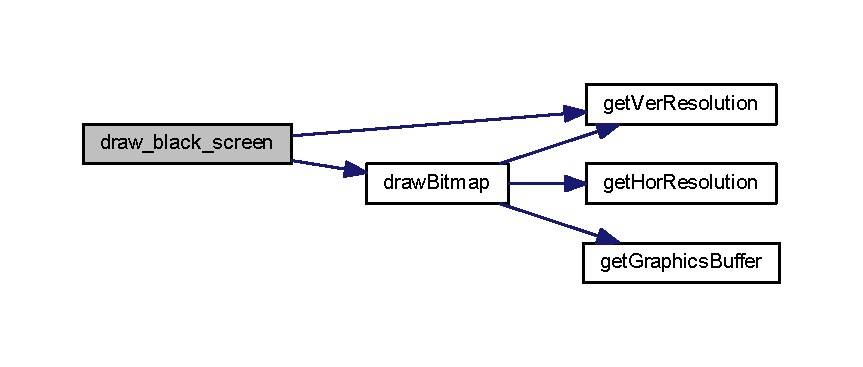
\includegraphics[width=350pt]{group___bitmap_ga66c6cdf9473527bd3dcbab53d147d5b9_cgraph}
\end{center}
\end{figure}
Here is the caller graph for this function\+:\nopagebreak
\begin{figure}[H]
\begin{center}
\leavevmode
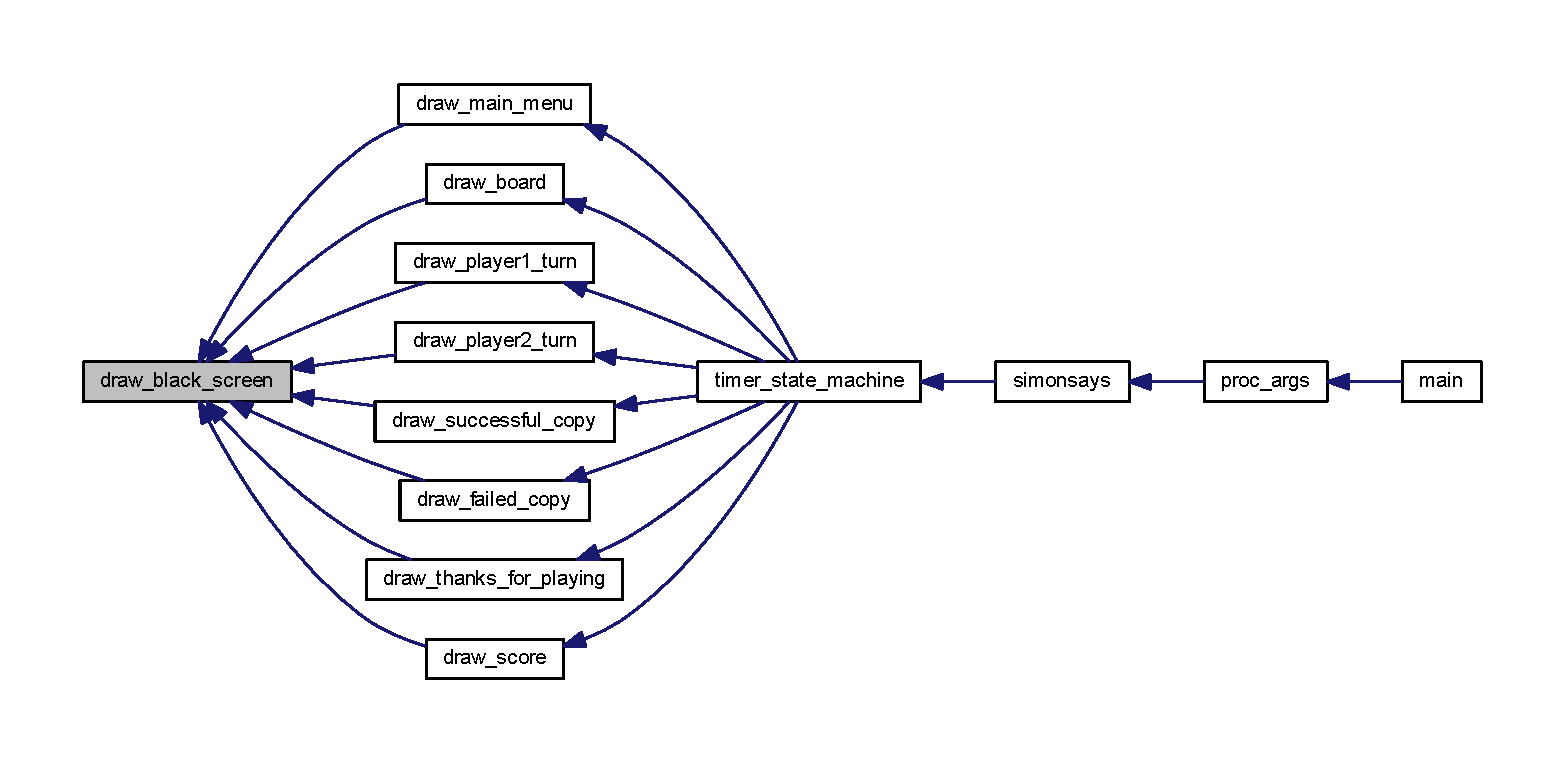
\includegraphics[width=350pt]{group___bitmap_ga66c6cdf9473527bd3dcbab53d147d5b9_icgraph}
\end{center}
\end{figure}
\mbox{\Hypertarget{group___bitmap_gaa7519d8a181750afa183c3350c5f9598}\label{group___bitmap_gaa7519d8a181750afa183c3350c5f9598}} 
\index{Bitmap@{Bitmap}!draw\+\_\+board@{draw\+\_\+board}}
\index{draw\+\_\+board@{draw\+\_\+board}!Bitmap@{Bitmap}}
\subsubsection{\texorpdfstring{draw\+\_\+board()}{draw\_board()}}
{\footnotesize\ttfamily void draw\+\_\+board (\begin{DoxyParamCaption}\item[{int}]{round }\end{DoxyParamCaption})}



Draws the game board, environment in wich the game will decurr (the gaming board shows the current round). 


\begin{DoxyParams}{Parameters}
{\em round} & current game round \\
\hline
\end{DoxyParams}
Here is the call graph for this function\+:\nopagebreak
\begin{figure}[H]
\begin{center}
\leavevmode
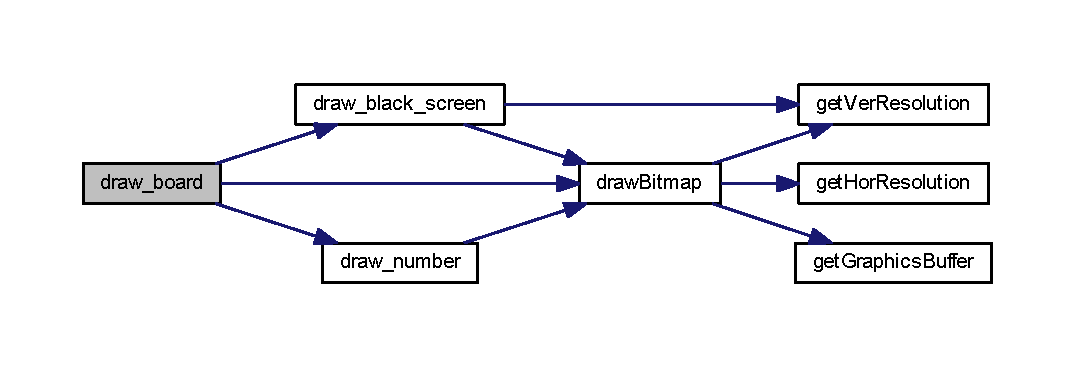
\includegraphics[width=350pt]{group___bitmap_gaa7519d8a181750afa183c3350c5f9598_cgraph}
\end{center}
\end{figure}
Here is the caller graph for this function\+:\nopagebreak
\begin{figure}[H]
\begin{center}
\leavevmode
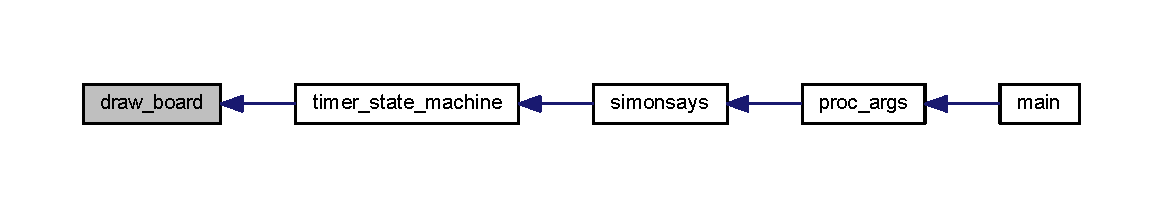
\includegraphics[width=350pt]{group___bitmap_gaa7519d8a181750afa183c3350c5f9598_icgraph}
\end{center}
\end{figure}
\mbox{\Hypertarget{group___bitmap_ga108608b0f2d804c84a271547036b6ffd}\label{group___bitmap_ga108608b0f2d804c84a271547036b6ffd}} 
\index{Bitmap@{Bitmap}!draw\+\_\+cursor@{draw\+\_\+cursor}}
\index{draw\+\_\+cursor@{draw\+\_\+cursor}!Bitmap@{Bitmap}}
\subsubsection{\texorpdfstring{draw\+\_\+cursor()}{draw\_cursor()}}
{\footnotesize\ttfamily void draw\+\_\+cursor (\begin{DoxyParamCaption}\item[{int}]{x,  }\item[{int}]{y }\end{DoxyParamCaption})}



Draws the mouse cursor at a given location. 


\begin{DoxyParams}{Parameters}
{\em x} & x coordinate of the location where the mouse cursor will be drawn \\
\hline
{\em y} & y coordinate of the location where the mouse cursor will be drawn \\
\hline
\end{DoxyParams}
Here is the call graph for this function\+:\nopagebreak
\begin{figure}[H]
\begin{center}
\leavevmode
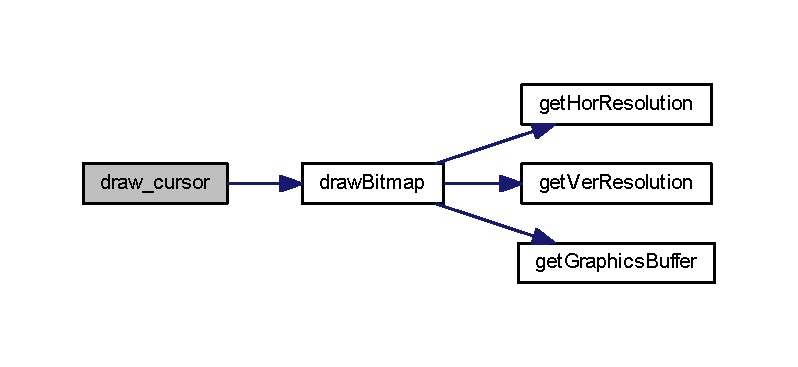
\includegraphics[width=350pt]{group___bitmap_ga108608b0f2d804c84a271547036b6ffd_cgraph}
\end{center}
\end{figure}
Here is the caller graph for this function\+:\nopagebreak
\begin{figure}[H]
\begin{center}
\leavevmode
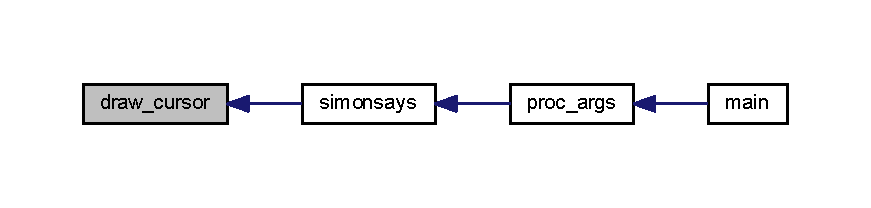
\includegraphics[width=350pt]{group___bitmap_ga108608b0f2d804c84a271547036b6ffd_icgraph}
\end{center}
\end{figure}
\mbox{\Hypertarget{group___bitmap_ga06ba1c351da1ccdfa323137861c1a9af}\label{group___bitmap_ga06ba1c351da1ccdfa323137861c1a9af}} 
\index{Bitmap@{Bitmap}!draw\+\_\+failed\+\_\+copy@{draw\+\_\+failed\+\_\+copy}}
\index{draw\+\_\+failed\+\_\+copy@{draw\+\_\+failed\+\_\+copy}!Bitmap@{Bitmap}}
\subsubsection{\texorpdfstring{draw\+\_\+failed\+\_\+copy()}{draw\_failed\_copy()}}
{\footnotesize\ttfamily void draw\+\_\+failed\+\_\+copy (\begin{DoxyParamCaption}{ }\end{DoxyParamCaption})}



A draw that announces a failed copy of player1\textquotesingle{}s moves. 

Here is the call graph for this function\+:\nopagebreak
\begin{figure}[H]
\begin{center}
\leavevmode
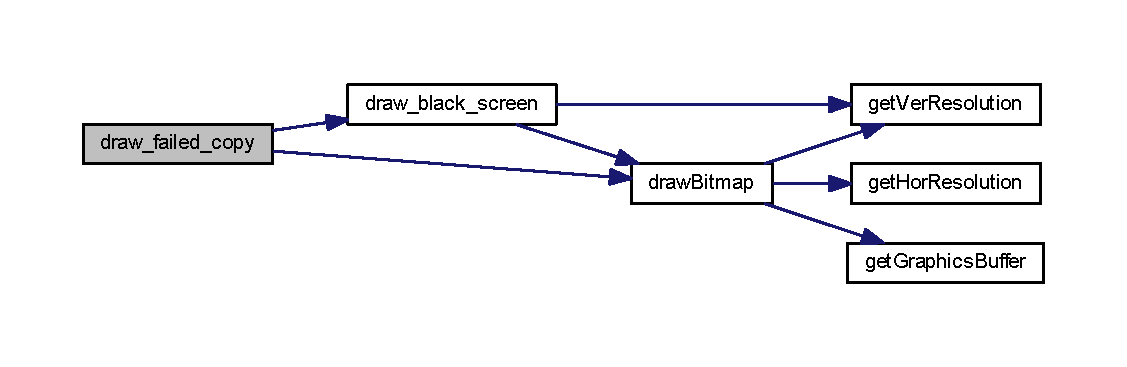
\includegraphics[width=350pt]{group___bitmap_ga06ba1c351da1ccdfa323137861c1a9af_cgraph}
\end{center}
\end{figure}
Here is the caller graph for this function\+:\nopagebreak
\begin{figure}[H]
\begin{center}
\leavevmode
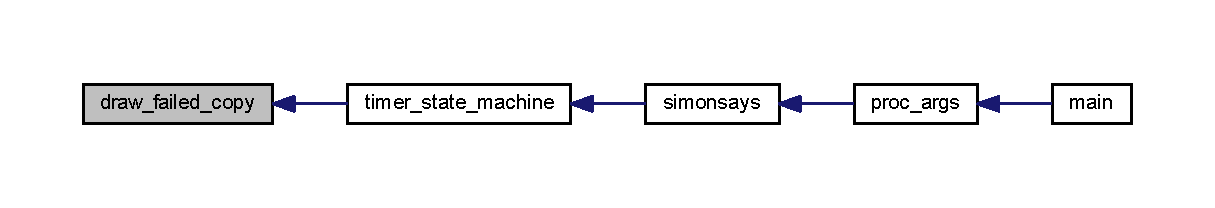
\includegraphics[width=350pt]{group___bitmap_ga06ba1c351da1ccdfa323137861c1a9af_icgraph}
\end{center}
\end{figure}
\mbox{\Hypertarget{group___bitmap_ga556f9cfc8664aff3169e9775310a5144}\label{group___bitmap_ga556f9cfc8664aff3169e9775310a5144}} 
\index{Bitmap@{Bitmap}!draw\+\_\+input@{draw\+\_\+input}}
\index{draw\+\_\+input@{draw\+\_\+input}!Bitmap@{Bitmap}}
\subsubsection{\texorpdfstring{draw\+\_\+input()}{draw\_input()}}
{\footnotesize\ttfamily void draw\+\_\+input (\begin{DoxyParamCaption}\item[{int}]{input }\end{DoxyParamCaption})}



A draws a given input given by a player. an input is a play made by a player (it can be selecting a geometrical figure on the board, preesing a key, or draw a positive slope with the mouse) 


\begin{DoxyParams}{Parameters}
{\em input} & play made by a player \\
\hline
\end{DoxyParams}
Here is the call graph for this function\+:\nopagebreak
\begin{figure}[H]
\begin{center}
\leavevmode
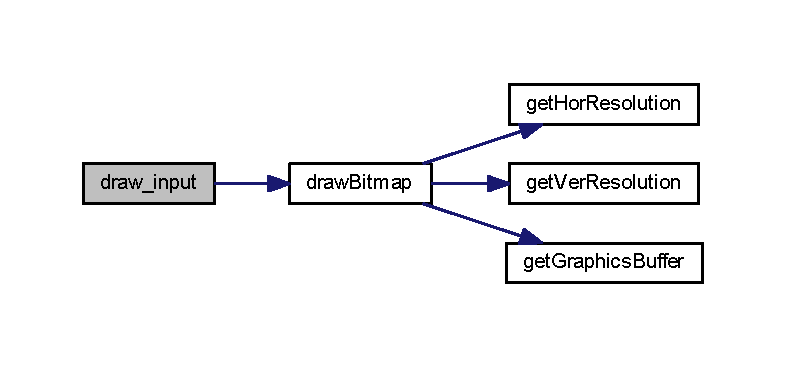
\includegraphics[width=350pt]{group___bitmap_ga556f9cfc8664aff3169e9775310a5144_cgraph}
\end{center}
\end{figure}
Here is the caller graph for this function\+:\nopagebreak
\begin{figure}[H]
\begin{center}
\leavevmode
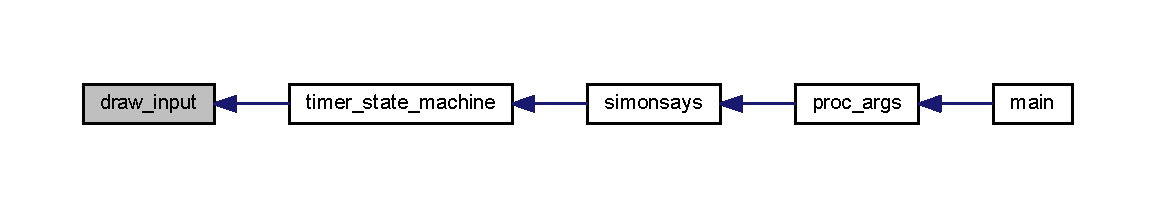
\includegraphics[width=350pt]{group___bitmap_ga556f9cfc8664aff3169e9775310a5144_icgraph}
\end{center}
\end{figure}
\mbox{\Hypertarget{group___bitmap_ga83361e027b6f0dd917305f1f82dedda3}\label{group___bitmap_ga83361e027b6f0dd917305f1f82dedda3}} 
\index{Bitmap@{Bitmap}!draw\+\_\+main\+\_\+menu@{draw\+\_\+main\+\_\+menu}}
\index{draw\+\_\+main\+\_\+menu@{draw\+\_\+main\+\_\+menu}!Bitmap@{Bitmap}}
\subsubsection{\texorpdfstring{draw\+\_\+main\+\_\+menu()}{draw\_main\_menu()}}
{\footnotesize\ttfamily void draw\+\_\+main\+\_\+menu (\begin{DoxyParamCaption}{ }\end{DoxyParamCaption})}



Draws the main menu, wich gives you two options\+: S\+T\+A\+RT or E\+X\+IT. 

Here is the call graph for this function\+:\nopagebreak
\begin{figure}[H]
\begin{center}
\leavevmode
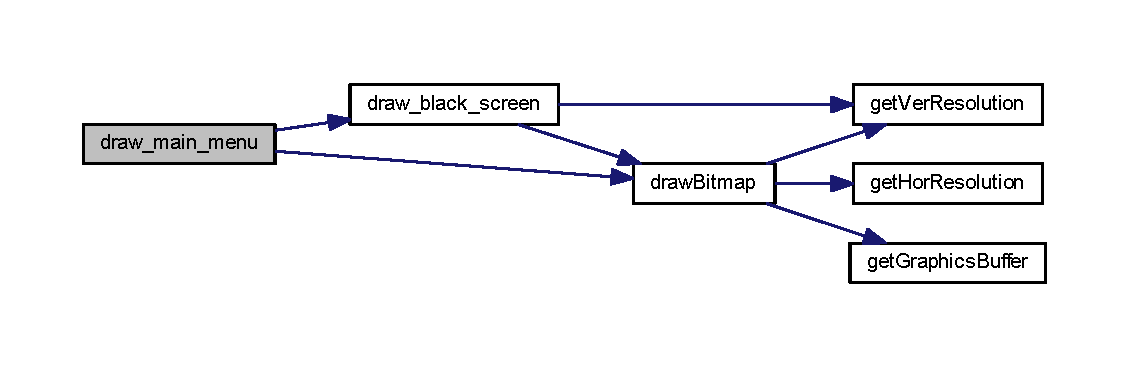
\includegraphics[width=350pt]{group___bitmap_ga83361e027b6f0dd917305f1f82dedda3_cgraph}
\end{center}
\end{figure}
Here is the caller graph for this function\+:\nopagebreak
\begin{figure}[H]
\begin{center}
\leavevmode
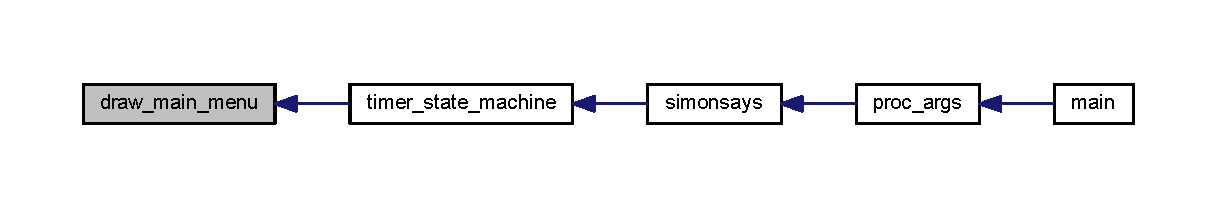
\includegraphics[width=350pt]{group___bitmap_ga83361e027b6f0dd917305f1f82dedda3_icgraph}
\end{center}
\end{figure}
\mbox{\Hypertarget{group___bitmap_ga97df0f6e4184d84c9e3871042b94bc3a}\label{group___bitmap_ga97df0f6e4184d84c9e3871042b94bc3a}} 
\index{Bitmap@{Bitmap}!draw\+\_\+number@{draw\+\_\+number}}
\index{draw\+\_\+number@{draw\+\_\+number}!Bitmap@{Bitmap}}
\subsubsection{\texorpdfstring{draw\+\_\+number()}{draw\_number()}}
{\footnotesize\ttfamily void draw\+\_\+number (\begin{DoxyParamCaption}\item[{int}]{number,  }\item[{int}]{x,  }\item[{int}]{y }\end{DoxyParamCaption})}



Draws a number(0-\/9) at a given location(x,y) 


\begin{DoxyParams}{Parameters}
{\em number} & number to be drawn \\
\hline
{\em x} & x coordinate where the number will be drawn \\
\hline
{\em y} & y coordinate where the number will be drawn \\
\hline
\end{DoxyParams}
Here is the call graph for this function\+:\nopagebreak
\begin{figure}[H]
\begin{center}
\leavevmode
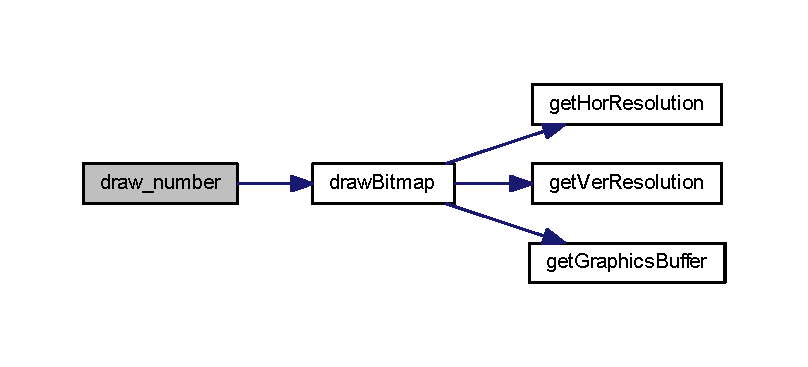
\includegraphics[width=350pt]{group___bitmap_ga97df0f6e4184d84c9e3871042b94bc3a_cgraph}
\end{center}
\end{figure}
Here is the caller graph for this function\+:\nopagebreak
\begin{figure}[H]
\begin{center}
\leavevmode
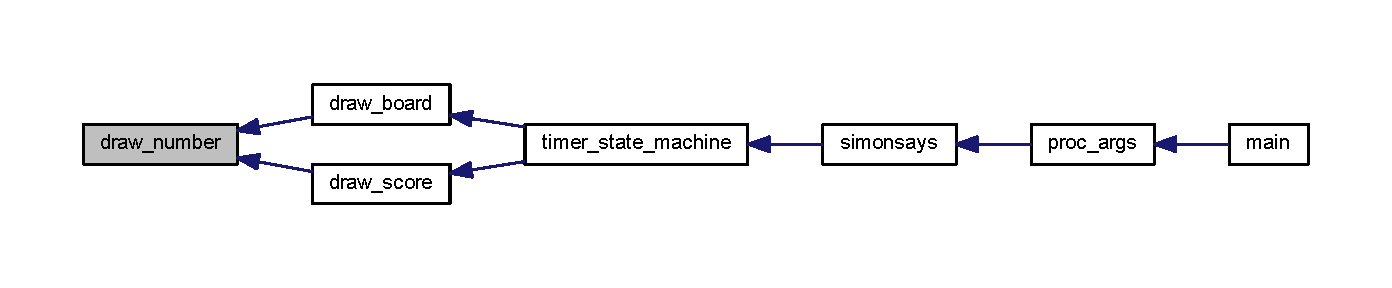
\includegraphics[width=350pt]{group___bitmap_ga97df0f6e4184d84c9e3871042b94bc3a_icgraph}
\end{center}
\end{figure}
\mbox{\Hypertarget{group___bitmap_gaca0d178c01fee283d1e3386b9712736e}\label{group___bitmap_gaca0d178c01fee283d1e3386b9712736e}} 
\index{Bitmap@{Bitmap}!draw\+\_\+player1\+\_\+turn@{draw\+\_\+player1\+\_\+turn}}
\index{draw\+\_\+player1\+\_\+turn@{draw\+\_\+player1\+\_\+turn}!Bitmap@{Bitmap}}
\subsubsection{\texorpdfstring{draw\+\_\+player1\+\_\+turn()}{draw\_player1\_turn()}}
{\footnotesize\ttfamily void draw\+\_\+player1\+\_\+turn (\begin{DoxyParamCaption}{ }\end{DoxyParamCaption})}



A draw that announces player1\textquotesingle{}s turn to play. 

Here is the call graph for this function\+:\nopagebreak
\begin{figure}[H]
\begin{center}
\leavevmode
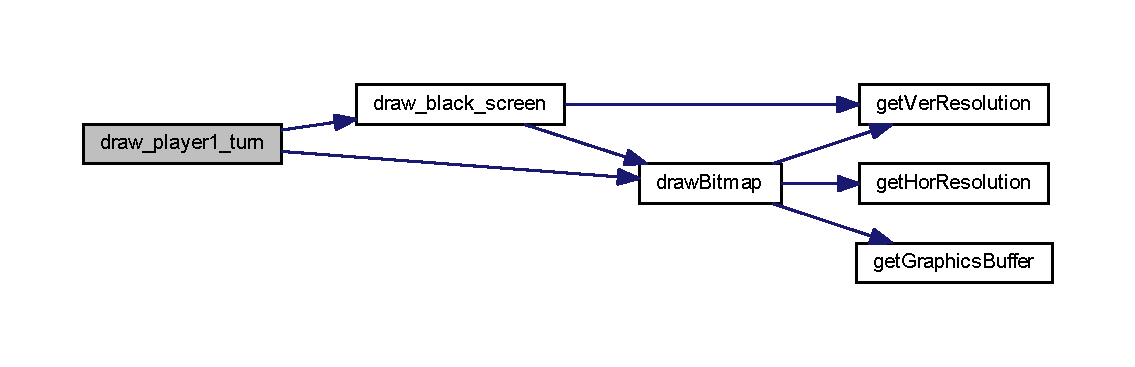
\includegraphics[width=350pt]{group___bitmap_gaca0d178c01fee283d1e3386b9712736e_cgraph}
\end{center}
\end{figure}
Here is the caller graph for this function\+:\nopagebreak
\begin{figure}[H]
\begin{center}
\leavevmode
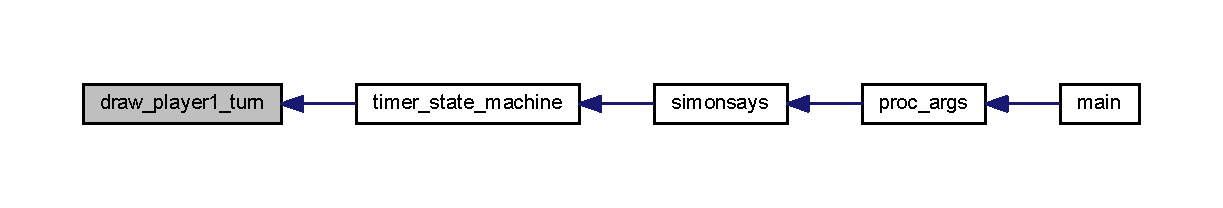
\includegraphics[width=350pt]{group___bitmap_gaca0d178c01fee283d1e3386b9712736e_icgraph}
\end{center}
\end{figure}
\mbox{\Hypertarget{group___bitmap_ga9af400ed66deb4c3aff712d9a7e9f522}\label{group___bitmap_ga9af400ed66deb4c3aff712d9a7e9f522}} 
\index{Bitmap@{Bitmap}!draw\+\_\+player2\+\_\+turn@{draw\+\_\+player2\+\_\+turn}}
\index{draw\+\_\+player2\+\_\+turn@{draw\+\_\+player2\+\_\+turn}!Bitmap@{Bitmap}}
\subsubsection{\texorpdfstring{draw\+\_\+player2\+\_\+turn()}{draw\_player2\_turn()}}
{\footnotesize\ttfamily void draw\+\_\+player2\+\_\+turn (\begin{DoxyParamCaption}{ }\end{DoxyParamCaption})}



A draw that announces player2\textquotesingle{}s turn to play. 

Here is the call graph for this function\+:\nopagebreak
\begin{figure}[H]
\begin{center}
\leavevmode
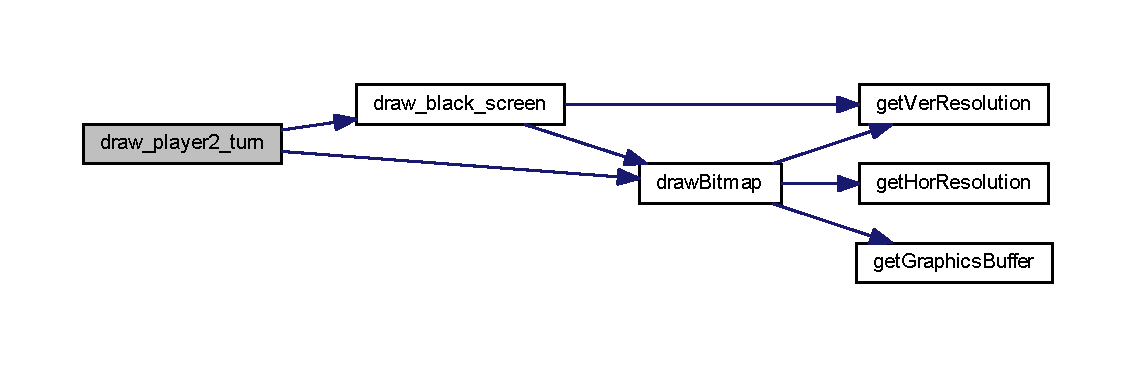
\includegraphics[width=350pt]{group___bitmap_ga9af400ed66deb4c3aff712d9a7e9f522_cgraph}
\end{center}
\end{figure}
Here is the caller graph for this function\+:\nopagebreak
\begin{figure}[H]
\begin{center}
\leavevmode
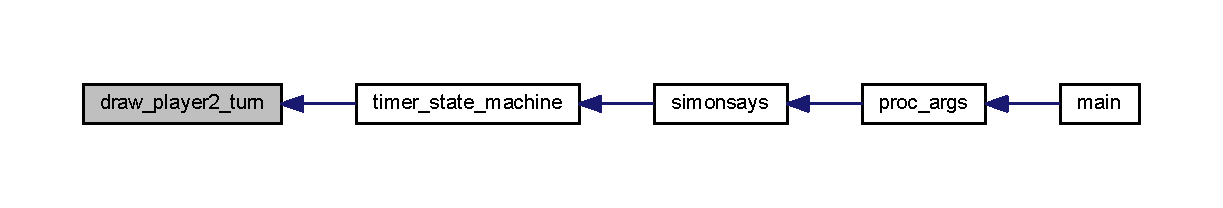
\includegraphics[width=350pt]{group___bitmap_ga9af400ed66deb4c3aff712d9a7e9f522_icgraph}
\end{center}
\end{figure}
\mbox{\Hypertarget{group___bitmap_gae696a3d4ee82a15e937f5f8c11fa9057}\label{group___bitmap_gae696a3d4ee82a15e937f5f8c11fa9057}} 
\index{Bitmap@{Bitmap}!draw\+\_\+success\+\_\+copy@{draw\+\_\+success\+\_\+copy}}
\index{draw\+\_\+success\+\_\+copy@{draw\+\_\+success\+\_\+copy}!Bitmap@{Bitmap}}
\subsubsection{\texorpdfstring{draw\+\_\+success\+\_\+copy()}{draw\_success\_copy()}}
{\footnotesize\ttfamily void draw\+\_\+success\+\_\+copy (\begin{DoxyParamCaption}{ }\end{DoxyParamCaption})}



A draw that announces a successful copy of player1\textquotesingle{}s moves. 

\mbox{\Hypertarget{group___bitmap_gabbf5153c909fc82e7734744352e22de9}\label{group___bitmap_gabbf5153c909fc82e7734744352e22de9}} 
\index{Bitmap@{Bitmap}!draw\+\_\+thanks\+\_\+for\+\_\+playing@{draw\+\_\+thanks\+\_\+for\+\_\+playing}}
\index{draw\+\_\+thanks\+\_\+for\+\_\+playing@{draw\+\_\+thanks\+\_\+for\+\_\+playing}!Bitmap@{Bitmap}}
\subsubsection{\texorpdfstring{draw\+\_\+thanks\+\_\+for\+\_\+playing()}{draw\_thanks\_for\_playing()}}
{\footnotesize\ttfamily void draw\+\_\+thanks\+\_\+for\+\_\+playing (\begin{DoxyParamCaption}{ }\end{DoxyParamCaption})}



A draw that says \char`\"{}\+Thank you for playing\char`\"{}. 

Here is the call graph for this function\+:\nopagebreak
\begin{figure}[H]
\begin{center}
\leavevmode
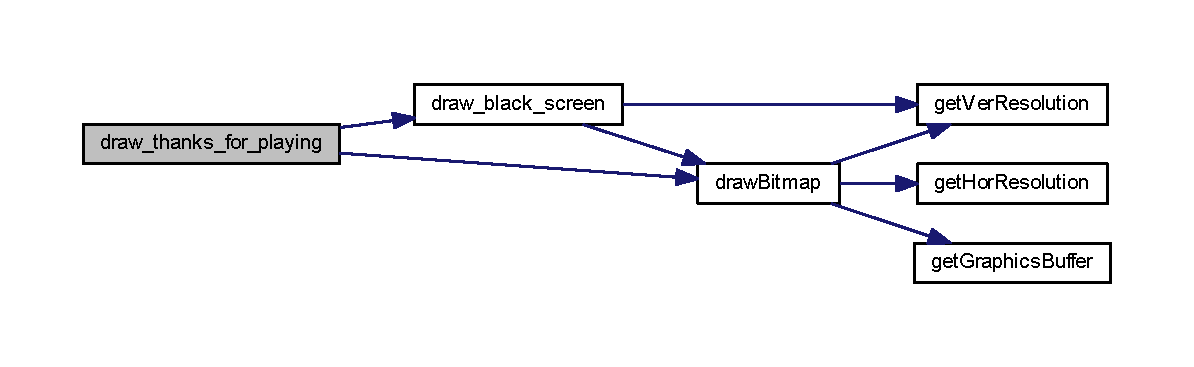
\includegraphics[width=350pt]{group___bitmap_gabbf5153c909fc82e7734744352e22de9_cgraph}
\end{center}
\end{figure}
Here is the caller graph for this function\+:\nopagebreak
\begin{figure}[H]
\begin{center}
\leavevmode
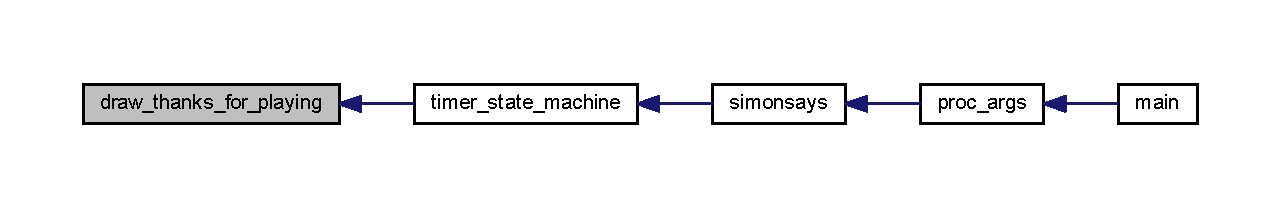
\includegraphics[width=350pt]{group___bitmap_gabbf5153c909fc82e7734744352e22de9_icgraph}
\end{center}
\end{figure}
\mbox{\Hypertarget{group___bitmap_ga18d05a1c671f4638bc63d37874efb9d4}\label{group___bitmap_ga18d05a1c671f4638bc63d37874efb9d4}} 
\index{Bitmap@{Bitmap}!draw\+Bitmap@{draw\+Bitmap}}
\index{draw\+Bitmap@{draw\+Bitmap}!Bitmap@{Bitmap}}
\subsubsection{\texorpdfstring{draw\+Bitmap()}{drawBitmap()}}
{\footnotesize\ttfamily void draw\+Bitmap (\begin{DoxyParamCaption}\item[{\hyperlink{struct_bitmap}{Bitmap} $\ast$}]{bitmap,  }\item[{int}]{x,  }\item[{int}]{y,  }\item[{\hyperlink{group___bitmap_gacdfaca60ec19c0265bac2692d7982726}{Alignment}}]{alignment }\end{DoxyParamCaption})}



Draws an unscaled, unrotated bitmap at the given position. 


\begin{DoxyParams}{Parameters}
{\em bitmap} & bitmap to be drawn \\
\hline
{\em x} & destiny x coord \\
\hline
{\em y} & destiny y coord \\
\hline
{\em alignment} & image alignment \\
\hline
\end{DoxyParams}
Here is the call graph for this function\+:\nopagebreak
\begin{figure}[H]
\begin{center}
\leavevmode
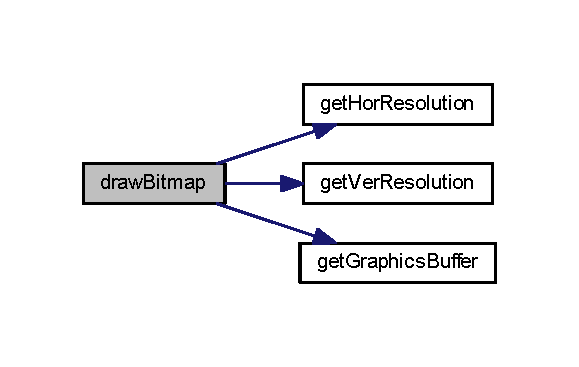
\includegraphics[width=278pt]{group___bitmap_ga18d05a1c671f4638bc63d37874efb9d4_cgraph}
\end{center}
\end{figure}
Here is the caller graph for this function\+:\nopagebreak
\begin{figure}[H]
\begin{center}
\leavevmode
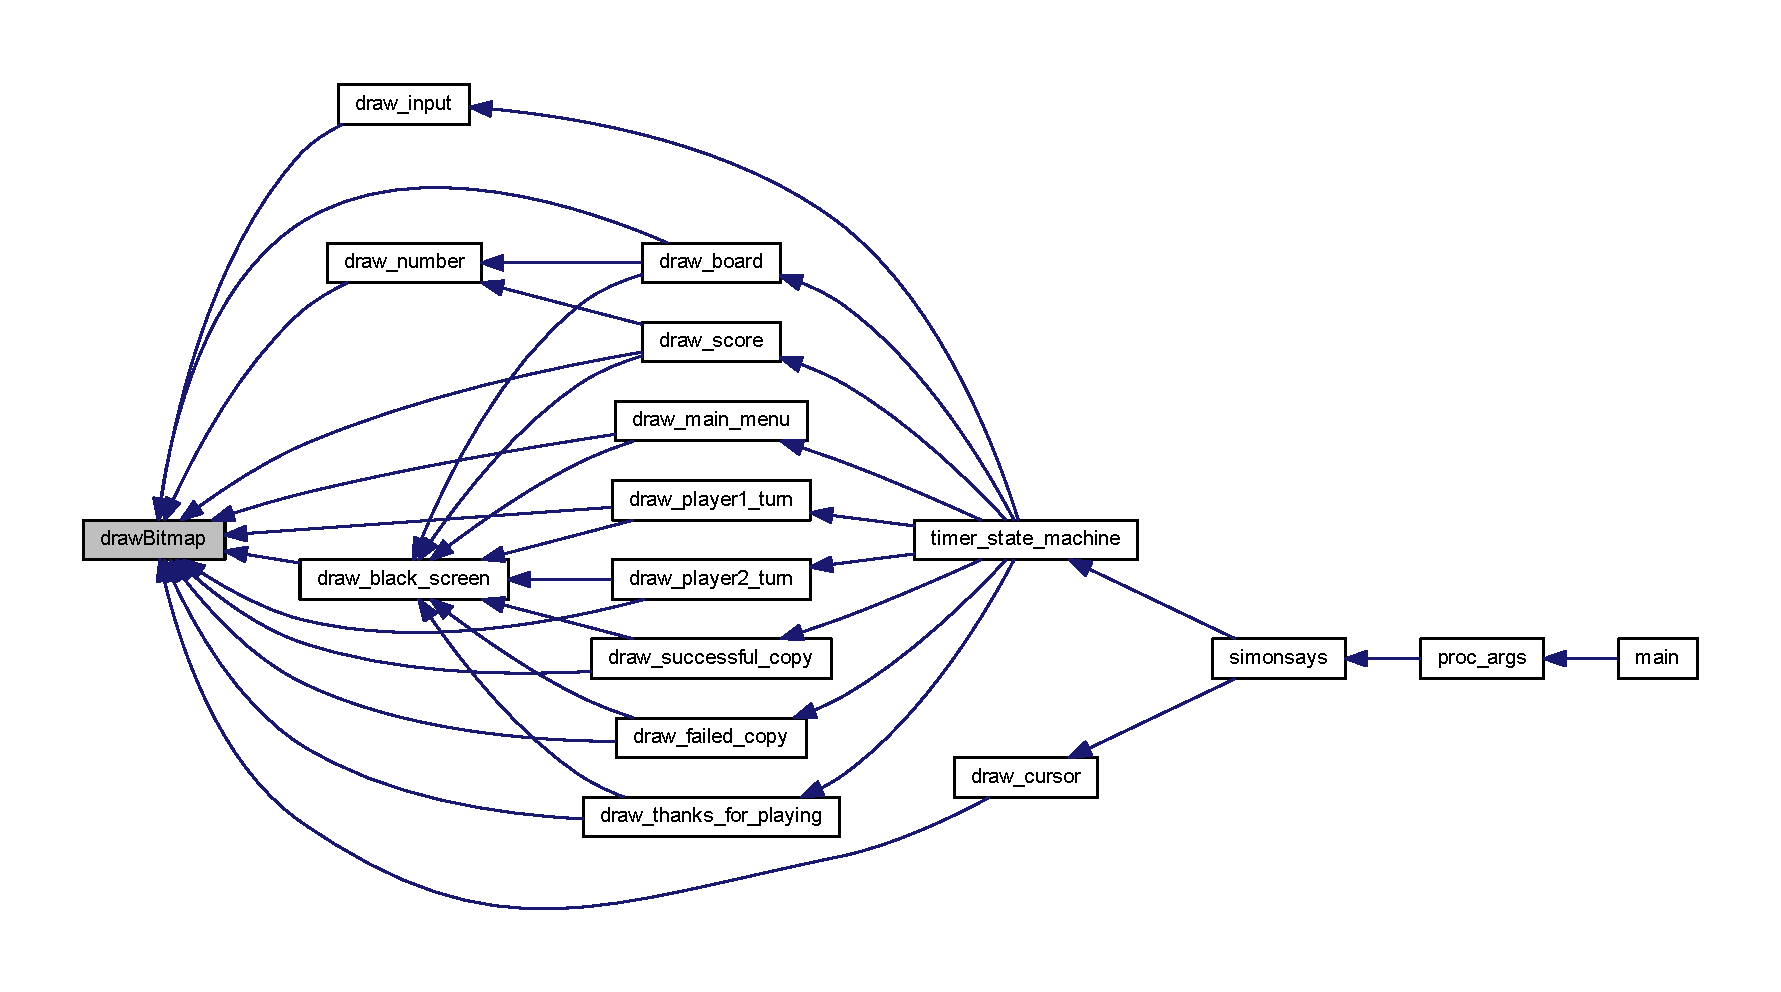
\includegraphics[width=350pt]{group___bitmap_ga18d05a1c671f4638bc63d37874efb9d4_icgraph}
\end{center}
\end{figure}
\mbox{\Hypertarget{group___bitmap_gabda6654c65348aa9c06a9ae0e9562b9a}\label{group___bitmap_gabda6654c65348aa9c06a9ae0e9562b9a}} 
\index{Bitmap@{Bitmap}!get\+\_\+bitmaps@{get\+\_\+bitmaps}}
\index{get\+\_\+bitmaps@{get\+\_\+bitmaps}!Bitmap@{Bitmap}}
\subsubsection{\texorpdfstring{get\+\_\+bitmaps()}{get\_bitmaps()}}
{\footnotesize\ttfamily void get\+\_\+bitmaps (\begin{DoxyParamCaption}{ }\end{DoxyParamCaption})}



Loads all the bitmaps used by calling load\+Bitmap function. 

Here is the call graph for this function\+:\nopagebreak
\begin{figure}[H]
\begin{center}
\leavevmode
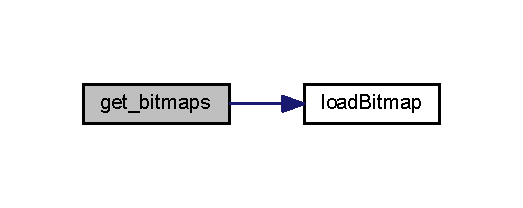
\includegraphics[width=251pt]{group___bitmap_gabda6654c65348aa9c06a9ae0e9562b9a_cgraph}
\end{center}
\end{figure}
Here is the caller graph for this function\+:\nopagebreak
\begin{figure}[H]
\begin{center}
\leavevmode
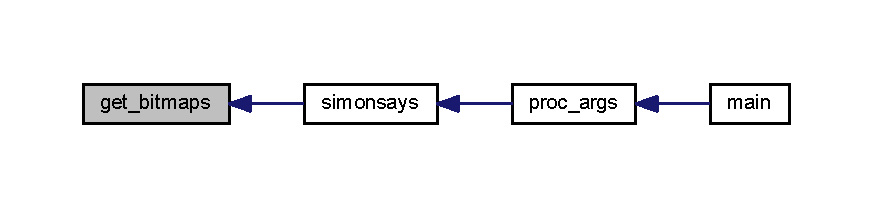
\includegraphics[width=350pt]{group___bitmap_gabda6654c65348aa9c06a9ae0e9562b9a_icgraph}
\end{center}
\end{figure}
\mbox{\Hypertarget{group___bitmap_ga3506880ffd407c36eb8aaddd2c1606d2}\label{group___bitmap_ga3506880ffd407c36eb8aaddd2c1606d2}} 
\index{Bitmap@{Bitmap}!load\+Bitmap@{load\+Bitmap}}
\index{load\+Bitmap@{load\+Bitmap}!Bitmap@{Bitmap}}
\subsubsection{\texorpdfstring{load\+Bitmap()}{loadBitmap()}}
{\footnotesize\ttfamily \hyperlink{struct_bitmap}{Bitmap}$\ast$ load\+Bitmap (\begin{DoxyParamCaption}\item[{const char $\ast$}]{filename }\end{DoxyParamCaption})}



Loads a bmp image. 


\begin{DoxyParams}{Parameters}
{\em filename} & Path of the image to load \\
\hline
\end{DoxyParams}
\begin{DoxyReturn}{Returns}
Non N\+U\+LL pointer to the image buffer 
\end{DoxyReturn}
Here is the caller graph for this function\+:\nopagebreak
\begin{figure}[H]
\begin{center}
\leavevmode
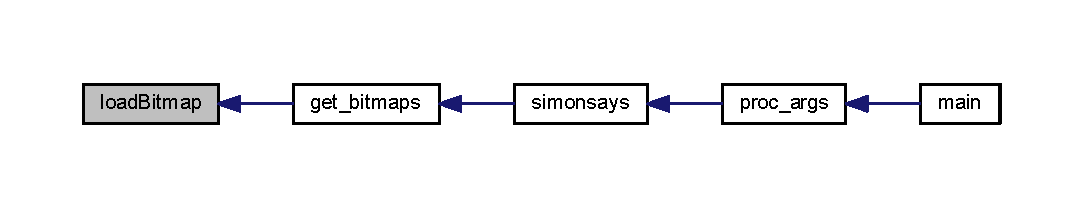
\includegraphics[width=350pt]{group___bitmap_ga3506880ffd407c36eb8aaddd2c1606d2_icgraph}
\end{center}
\end{figure}


\subsection{Variable Documentation}
\mbox{\Hypertarget{group___bitmap_ga508d397d656733b6434a84217519cf27}\label{group___bitmap_ga508d397d656733b6434a84217519cf27}} 
\index{Bitmap@{Bitmap}!bitmap\+\_\+a\+\_\+key@{bitmap\+\_\+a\+\_\+key}}
\index{bitmap\+\_\+a\+\_\+key@{bitmap\+\_\+a\+\_\+key}!Bitmap@{Bitmap}}
\subsubsection{\texorpdfstring{bitmap\+\_\+a\+\_\+key}{bitmap\_a\_key}}
{\footnotesize\ttfamily \hyperlink{struct_bitmap}{Bitmap}$\ast$ bitmap\+\_\+a\+\_\+key}

\mbox{\Hypertarget{group___bitmap_ga25ccce5a865640e111d5c3e6fd8405f5}\label{group___bitmap_ga25ccce5a865640e111d5c3e6fd8405f5}} 
\index{Bitmap@{Bitmap}!bitmap\+\_\+black\+\_\+bar@{bitmap\+\_\+black\+\_\+bar}}
\index{bitmap\+\_\+black\+\_\+bar@{bitmap\+\_\+black\+\_\+bar}!Bitmap@{Bitmap}}
\subsubsection{\texorpdfstring{bitmap\+\_\+black\+\_\+bar}{bitmap\_black\_bar}}
{\footnotesize\ttfamily \hyperlink{struct_bitmap}{Bitmap}$\ast$ bitmap\+\_\+black\+\_\+bar}

\mbox{\Hypertarget{group___bitmap_ga3a3b4fedabcc22d1b0f34e651fcfdb46}\label{group___bitmap_ga3a3b4fedabcc22d1b0f34e651fcfdb46}} 
\index{Bitmap@{Bitmap}!bitmap\+\_\+black\+\_\+square@{bitmap\+\_\+black\+\_\+square}}
\index{bitmap\+\_\+black\+\_\+square@{bitmap\+\_\+black\+\_\+square}!Bitmap@{Bitmap}}
\subsubsection{\texorpdfstring{bitmap\+\_\+black\+\_\+square}{bitmap\_black\_square}}
{\footnotesize\ttfamily \hyperlink{struct_bitmap}{Bitmap}$\ast$ bitmap\+\_\+black\+\_\+square}

\mbox{\Hypertarget{group___bitmap_gac1d843b74dd56e98adf0c72f75a5a1d8}\label{group___bitmap_gac1d843b74dd56e98adf0c72f75a5a1d8}} 
\index{Bitmap@{Bitmap}!bitmap\+\_\+circle@{bitmap\+\_\+circle}}
\index{bitmap\+\_\+circle@{bitmap\+\_\+circle}!Bitmap@{Bitmap}}
\subsubsection{\texorpdfstring{bitmap\+\_\+circle}{bitmap\_circle}}
{\footnotesize\ttfamily \hyperlink{struct_bitmap}{Bitmap}$\ast$ bitmap\+\_\+circle}

\mbox{\Hypertarget{group___bitmap_ga1f04a1ac0e8402f5de2230baf1f6818d}\label{group___bitmap_ga1f04a1ac0e8402f5de2230baf1f6818d}} 
\index{Bitmap@{Bitmap}!bitmap\+\_\+congratulations@{bitmap\+\_\+congratulations}}
\index{bitmap\+\_\+congratulations@{bitmap\+\_\+congratulations}!Bitmap@{Bitmap}}
\subsubsection{\texorpdfstring{bitmap\+\_\+congratulations}{bitmap\_congratulations}}
{\footnotesize\ttfamily \hyperlink{struct_bitmap}{Bitmap}$\ast$ bitmap\+\_\+congratulations}

\mbox{\Hypertarget{group___bitmap_ga4eb982d201096abdac3cacd3f6459ff2}\label{group___bitmap_ga4eb982d201096abdac3cacd3f6459ff2}} 
\index{Bitmap@{Bitmap}!bitmap\+\_\+cpu@{bitmap\+\_\+cpu}}
\index{bitmap\+\_\+cpu@{bitmap\+\_\+cpu}!Bitmap@{Bitmap}}
\subsubsection{\texorpdfstring{bitmap\+\_\+cpu}{bitmap\_cpu}}
{\footnotesize\ttfamily \hyperlink{struct_bitmap}{Bitmap}$\ast$ bitmap\+\_\+cpu}

\mbox{\Hypertarget{group___bitmap_gae897f24816ba9a98f564b2b7ff488bc2}\label{group___bitmap_gae897f24816ba9a98f564b2b7ff488bc2}} 
\index{Bitmap@{Bitmap}!bitmap\+\_\+cursor@{bitmap\+\_\+cursor}}
\index{bitmap\+\_\+cursor@{bitmap\+\_\+cursor}!Bitmap@{Bitmap}}
\subsubsection{\texorpdfstring{bitmap\+\_\+cursor}{bitmap\_cursor}}
{\footnotesize\ttfamily \hyperlink{struct_bitmap}{Bitmap}$\ast$ bitmap\+\_\+cursor}

\mbox{\Hypertarget{group___bitmap_ga3887cbeee8746670c47e70090cc926ae}\label{group___bitmap_ga3887cbeee8746670c47e70090cc926ae}} 
\index{Bitmap@{Bitmap}!bitmap\+\_\+d\+\_\+key@{bitmap\+\_\+d\+\_\+key}}
\index{bitmap\+\_\+d\+\_\+key@{bitmap\+\_\+d\+\_\+key}!Bitmap@{Bitmap}}
\subsubsection{\texorpdfstring{bitmap\+\_\+d\+\_\+key}{bitmap\_d\_key}}
{\footnotesize\ttfamily \hyperlink{struct_bitmap}{Bitmap}$\ast$ bitmap\+\_\+d\+\_\+key}

\mbox{\Hypertarget{group___bitmap_ga952f653fe87f4ca995595e2b7db6228f}\label{group___bitmap_ga952f653fe87f4ca995595e2b7db6228f}} 
\index{Bitmap@{Bitmap}!bitmap\+\_\+exit@{bitmap\+\_\+exit}}
\index{bitmap\+\_\+exit@{bitmap\+\_\+exit}!Bitmap@{Bitmap}}
\subsubsection{\texorpdfstring{bitmap\+\_\+exit}{bitmap\_exit}}
{\footnotesize\ttfamily \hyperlink{struct_bitmap}{Bitmap}$\ast$ bitmap\+\_\+exit}

\mbox{\Hypertarget{group___bitmap_ga5d96b14aaf8cbac173f6d809be1ff7d4}\label{group___bitmap_ga5d96b14aaf8cbac173f6d809be1ff7d4}} 
\index{Bitmap@{Bitmap}!bitmap\+\_\+failed@{bitmap\+\_\+failed}}
\index{bitmap\+\_\+failed@{bitmap\+\_\+failed}!Bitmap@{Bitmap}}
\subsubsection{\texorpdfstring{bitmap\+\_\+failed}{bitmap\_failed}}
{\footnotesize\ttfamily \hyperlink{struct_bitmap}{Bitmap}$\ast$ bitmap\+\_\+failed}

\mbox{\Hypertarget{group___bitmap_gacb59d00d1a96d8b830bddde99bc4f7dd}\label{group___bitmap_gacb59d00d1a96d8b830bddde99bc4f7dd}} 
\index{Bitmap@{Bitmap}!bitmap\+\_\+final\+\_\+score@{bitmap\+\_\+final\+\_\+score}}
\index{bitmap\+\_\+final\+\_\+score@{bitmap\+\_\+final\+\_\+score}!Bitmap@{Bitmap}}
\subsubsection{\texorpdfstring{bitmap\+\_\+final\+\_\+score}{bitmap\_final\_score}}
{\footnotesize\ttfamily \hyperlink{struct_bitmap}{Bitmap}$\ast$ bitmap\+\_\+final\+\_\+score}

\mbox{\Hypertarget{group___bitmap_ga04b3490379f60798e7a6de171979a90f}\label{group___bitmap_ga04b3490379f60798e7a6de171979a90f}} 
\index{Bitmap@{Bitmap}!bitmap\+\_\+for@{bitmap\+\_\+for}}
\index{bitmap\+\_\+for@{bitmap\+\_\+for}!Bitmap@{Bitmap}}
\subsubsection{\texorpdfstring{bitmap\+\_\+for}{bitmap\_for}}
{\footnotesize\ttfamily \hyperlink{struct_bitmap}{Bitmap}$\ast$ bitmap\+\_\+for}

\mbox{\Hypertarget{group___bitmap_ga47000f83189d2a2f74f1148050ee338b}\label{group___bitmap_ga47000f83189d2a2f74f1148050ee338b}} 
\index{Bitmap@{Bitmap}!bitmap\+\_\+happy\+\_\+face@{bitmap\+\_\+happy\+\_\+face}}
\index{bitmap\+\_\+happy\+\_\+face@{bitmap\+\_\+happy\+\_\+face}!Bitmap@{Bitmap}}
\subsubsection{\texorpdfstring{bitmap\+\_\+happy\+\_\+face}{bitmap\_happy\_face}}
{\footnotesize\ttfamily \hyperlink{struct_bitmap}{Bitmap}$\ast$ bitmap\+\_\+happy\+\_\+face}

\mbox{\Hypertarget{group___bitmap_ga4610248f579630fea652a3704556c74c}\label{group___bitmap_ga4610248f579630fea652a3704556c74c}} 
\index{Bitmap@{Bitmap}!bitmap\+\_\+horizontal\+\_\+white\+\_\+bar@{bitmap\+\_\+horizontal\+\_\+white\+\_\+bar}}
\index{bitmap\+\_\+horizontal\+\_\+white\+\_\+bar@{bitmap\+\_\+horizontal\+\_\+white\+\_\+bar}!Bitmap@{Bitmap}}
\subsubsection{\texorpdfstring{bitmap\+\_\+horizontal\+\_\+white\+\_\+bar}{bitmap\_horizontal\_white\_bar}}
{\footnotesize\ttfamily \hyperlink{struct_bitmap}{Bitmap}$\ast$ bitmap\+\_\+horizontal\+\_\+white\+\_\+bar}

\mbox{\Hypertarget{group___bitmap_gac6d8af40b0549ee19c8d2d146ac2844f}\label{group___bitmap_gac6d8af40b0549ee19c8d2d146ac2844f}} 
\index{Bitmap@{Bitmap}!bitmap\+\_\+last\+\_\+input@{bitmap\+\_\+last\+\_\+input}}
\index{bitmap\+\_\+last\+\_\+input@{bitmap\+\_\+last\+\_\+input}!Bitmap@{Bitmap}}
\subsubsection{\texorpdfstring{bitmap\+\_\+last\+\_\+input}{bitmap\_last\_input}}
{\footnotesize\ttfamily \hyperlink{struct_bitmap}{Bitmap}$\ast$ bitmap\+\_\+last\+\_\+input}

\mbox{\Hypertarget{group___bitmap_gaf4ba721599394ebe28ce58f495fa1226}\label{group___bitmap_gaf4ba721599394ebe28ce58f495fa1226}} 
\index{Bitmap@{Bitmap}!bitmap\+\_\+nice@{bitmap\+\_\+nice}}
\index{bitmap\+\_\+nice@{bitmap\+\_\+nice}!Bitmap@{Bitmap}}
\subsubsection{\texorpdfstring{bitmap\+\_\+nice}{bitmap\_nice}}
{\footnotesize\ttfamily \hyperlink{struct_bitmap}{Bitmap}$\ast$ bitmap\+\_\+nice}

\mbox{\Hypertarget{group___bitmap_ga993712c0e2465ddf6682e1da844cb33f}\label{group___bitmap_ga993712c0e2465ddf6682e1da844cb33f}} 
\index{Bitmap@{Bitmap}!bitmap\+\_\+number\+\_\+0@{bitmap\+\_\+number\+\_\+0}}
\index{bitmap\+\_\+number\+\_\+0@{bitmap\+\_\+number\+\_\+0}!Bitmap@{Bitmap}}
\subsubsection{\texorpdfstring{bitmap\+\_\+number\+\_\+0}{bitmap\_number\_0}}
{\footnotesize\ttfamily \hyperlink{struct_bitmap}{Bitmap}$\ast$ bitmap\+\_\+number\+\_\+0}

\mbox{\Hypertarget{group___bitmap_gae0e099ab280db078712dae7370590d69}\label{group___bitmap_gae0e099ab280db078712dae7370590d69}} 
\index{Bitmap@{Bitmap}!bitmap\+\_\+number\+\_\+1@{bitmap\+\_\+number\+\_\+1}}
\index{bitmap\+\_\+number\+\_\+1@{bitmap\+\_\+number\+\_\+1}!Bitmap@{Bitmap}}
\subsubsection{\texorpdfstring{bitmap\+\_\+number\+\_\+1}{bitmap\_number\_1}}
{\footnotesize\ttfamily \hyperlink{struct_bitmap}{Bitmap}$\ast$ bitmap\+\_\+number\+\_\+1}

\mbox{\Hypertarget{group___bitmap_gabff0396d599ff9c20dc45260ac0023e3}\label{group___bitmap_gabff0396d599ff9c20dc45260ac0023e3}} 
\index{Bitmap@{Bitmap}!bitmap\+\_\+number\+\_\+2@{bitmap\+\_\+number\+\_\+2}}
\index{bitmap\+\_\+number\+\_\+2@{bitmap\+\_\+number\+\_\+2}!Bitmap@{Bitmap}}
\subsubsection{\texorpdfstring{bitmap\+\_\+number\+\_\+2}{bitmap\_number\_2}}
{\footnotesize\ttfamily \hyperlink{struct_bitmap}{Bitmap}$\ast$ bitmap\+\_\+number\+\_\+2}

\mbox{\Hypertarget{group___bitmap_ga691847399b96e5814e96eaa88d89a565}\label{group___bitmap_ga691847399b96e5814e96eaa88d89a565}} 
\index{Bitmap@{Bitmap}!bitmap\+\_\+number\+\_\+3@{bitmap\+\_\+number\+\_\+3}}
\index{bitmap\+\_\+number\+\_\+3@{bitmap\+\_\+number\+\_\+3}!Bitmap@{Bitmap}}
\subsubsection{\texorpdfstring{bitmap\+\_\+number\+\_\+3}{bitmap\_number\_3}}
{\footnotesize\ttfamily \hyperlink{struct_bitmap}{Bitmap}$\ast$ bitmap\+\_\+number\+\_\+3}

\mbox{\Hypertarget{group___bitmap_ga0d04224487333eb3e7b5e2f6f84c0c7c}\label{group___bitmap_ga0d04224487333eb3e7b5e2f6f84c0c7c}} 
\index{Bitmap@{Bitmap}!bitmap\+\_\+number\+\_\+4@{bitmap\+\_\+number\+\_\+4}}
\index{bitmap\+\_\+number\+\_\+4@{bitmap\+\_\+number\+\_\+4}!Bitmap@{Bitmap}}
\subsubsection{\texorpdfstring{bitmap\+\_\+number\+\_\+4}{bitmap\_number\_4}}
{\footnotesize\ttfamily \hyperlink{struct_bitmap}{Bitmap}$\ast$ bitmap\+\_\+number\+\_\+4}

\mbox{\Hypertarget{group___bitmap_ga2462605cb4d4dee9006653ffafe12fbc}\label{group___bitmap_ga2462605cb4d4dee9006653ffafe12fbc}} 
\index{Bitmap@{Bitmap}!bitmap\+\_\+number\+\_\+5@{bitmap\+\_\+number\+\_\+5}}
\index{bitmap\+\_\+number\+\_\+5@{bitmap\+\_\+number\+\_\+5}!Bitmap@{Bitmap}}
\subsubsection{\texorpdfstring{bitmap\+\_\+number\+\_\+5}{bitmap\_number\_5}}
{\footnotesize\ttfamily \hyperlink{struct_bitmap}{Bitmap}$\ast$ bitmap\+\_\+number\+\_\+5}

\mbox{\Hypertarget{group___bitmap_ga70b99f25995d8138d51132de297e66ba}\label{group___bitmap_ga70b99f25995d8138d51132de297e66ba}} 
\index{Bitmap@{Bitmap}!bitmap\+\_\+number\+\_\+6@{bitmap\+\_\+number\+\_\+6}}
\index{bitmap\+\_\+number\+\_\+6@{bitmap\+\_\+number\+\_\+6}!Bitmap@{Bitmap}}
\subsubsection{\texorpdfstring{bitmap\+\_\+number\+\_\+6}{bitmap\_number\_6}}
{\footnotesize\ttfamily \hyperlink{struct_bitmap}{Bitmap}$\ast$ bitmap\+\_\+number\+\_\+6}

\mbox{\Hypertarget{group___bitmap_ga8c4df34a71fbac148bc9ace8ba6095fa}\label{group___bitmap_ga8c4df34a71fbac148bc9ace8ba6095fa}} 
\index{Bitmap@{Bitmap}!bitmap\+\_\+number\+\_\+7@{bitmap\+\_\+number\+\_\+7}}
\index{bitmap\+\_\+number\+\_\+7@{bitmap\+\_\+number\+\_\+7}!Bitmap@{Bitmap}}
\subsubsection{\texorpdfstring{bitmap\+\_\+number\+\_\+7}{bitmap\_number\_7}}
{\footnotesize\ttfamily \hyperlink{struct_bitmap}{Bitmap}$\ast$ bitmap\+\_\+number\+\_\+7}

\mbox{\Hypertarget{group___bitmap_ga0b28cdc22a12665fb94f55d1c9d269f2}\label{group___bitmap_ga0b28cdc22a12665fb94f55d1c9d269f2}} 
\index{Bitmap@{Bitmap}!bitmap\+\_\+number\+\_\+8@{bitmap\+\_\+number\+\_\+8}}
\index{bitmap\+\_\+number\+\_\+8@{bitmap\+\_\+number\+\_\+8}!Bitmap@{Bitmap}}
\subsubsection{\texorpdfstring{bitmap\+\_\+number\+\_\+8}{bitmap\_number\_8}}
{\footnotesize\ttfamily \hyperlink{struct_bitmap}{Bitmap}$\ast$ bitmap\+\_\+number\+\_\+8}

\mbox{\Hypertarget{group___bitmap_ga8af434fd1017cdac47579582bac12552}\label{group___bitmap_ga8af434fd1017cdac47579582bac12552}} 
\index{Bitmap@{Bitmap}!bitmap\+\_\+number\+\_\+9@{bitmap\+\_\+number\+\_\+9}}
\index{bitmap\+\_\+number\+\_\+9@{bitmap\+\_\+number\+\_\+9}!Bitmap@{Bitmap}}
\subsubsection{\texorpdfstring{bitmap\+\_\+number\+\_\+9}{bitmap\_number\_9}}
{\footnotesize\ttfamily \hyperlink{struct_bitmap}{Bitmap}$\ast$ bitmap\+\_\+number\+\_\+9}

\mbox{\Hypertarget{group___bitmap_ga68d193359f4b1253056be87ab752f5f0}\label{group___bitmap_ga68d193359f4b1253056be87ab752f5f0}} 
\index{Bitmap@{Bitmap}!bitmap\+\_\+plagiarism@{bitmap\+\_\+plagiarism}}
\index{bitmap\+\_\+plagiarism@{bitmap\+\_\+plagiarism}!Bitmap@{Bitmap}}
\subsubsection{\texorpdfstring{bitmap\+\_\+plagiarism}{bitmap\_plagiarism}}
{\footnotesize\ttfamily \hyperlink{struct_bitmap}{Bitmap}$\ast$ bitmap\+\_\+plagiarism}

\mbox{\Hypertarget{group___bitmap_ga2ba19da7f92ccbe27fd209c98816837a}\label{group___bitmap_ga2ba19da7f92ccbe27fd209c98816837a}} 
\index{Bitmap@{Bitmap}!bitmap\+\_\+player1@{bitmap\+\_\+player1}}
\index{bitmap\+\_\+player1@{bitmap\+\_\+player1}!Bitmap@{Bitmap}}
\subsubsection{\texorpdfstring{bitmap\+\_\+player1}{bitmap\_player1}}
{\footnotesize\ttfamily \hyperlink{struct_bitmap}{Bitmap}$\ast$ bitmap\+\_\+player1}

\mbox{\Hypertarget{group___bitmap_ga63e9b3ca144cce02448900ffe9add6c4}\label{group___bitmap_ga63e9b3ca144cce02448900ffe9add6c4}} 
\index{Bitmap@{Bitmap}!bitmap\+\_\+player2@{bitmap\+\_\+player2}}
\index{bitmap\+\_\+player2@{bitmap\+\_\+player2}!Bitmap@{Bitmap}}
\subsubsection{\texorpdfstring{bitmap\+\_\+player2}{bitmap\_player2}}
{\footnotesize\ttfamily \hyperlink{struct_bitmap}{Bitmap}$\ast$ bitmap\+\_\+player2}

\mbox{\Hypertarget{group___bitmap_ga57060e5b51d9603d9fc393526c965a3b}\label{group___bitmap_ga57060e5b51d9603d9fc393526c965a3b}} 
\index{Bitmap@{Bitmap}!bitmap\+\_\+playing@{bitmap\+\_\+playing}}
\index{bitmap\+\_\+playing@{bitmap\+\_\+playing}!Bitmap@{Bitmap}}
\subsubsection{\texorpdfstring{bitmap\+\_\+playing}{bitmap\_playing}}
{\footnotesize\ttfamily \hyperlink{struct_bitmap}{Bitmap}$\ast$ bitmap\+\_\+playing}

\mbox{\Hypertarget{group___bitmap_ga2f913b78a0f833c9a04aef7f4b334062}\label{group___bitmap_ga2f913b78a0f833c9a04aef7f4b334062}} 
\index{Bitmap@{Bitmap}!bitmap\+\_\+round@{bitmap\+\_\+round}}
\index{bitmap\+\_\+round@{bitmap\+\_\+round}!Bitmap@{Bitmap}}
\subsubsection{\texorpdfstring{bitmap\+\_\+round}{bitmap\_round}}
{\footnotesize\ttfamily \hyperlink{struct_bitmap}{Bitmap}$\ast$ bitmap\+\_\+round}

\mbox{\Hypertarget{group___bitmap_gaec5fd5db7147e57f72076387bc78ffc9}\label{group___bitmap_gaec5fd5db7147e57f72076387bc78ffc9}} 
\index{Bitmap@{Bitmap}!bitmap\+\_\+s\+\_\+key@{bitmap\+\_\+s\+\_\+key}}
\index{bitmap\+\_\+s\+\_\+key@{bitmap\+\_\+s\+\_\+key}!Bitmap@{Bitmap}}
\subsubsection{\texorpdfstring{bitmap\+\_\+s\+\_\+key}{bitmap\_s\_key}}
{\footnotesize\ttfamily \hyperlink{struct_bitmap}{Bitmap}$\ast$ bitmap\+\_\+s\+\_\+key}

\mbox{\Hypertarget{group___bitmap_ga712c5447dd57d83342185a9ac9ca7015}\label{group___bitmap_ga712c5447dd57d83342185a9ac9ca7015}} 
\index{Bitmap@{Bitmap}!bitmap\+\_\+sad\+\_\+face@{bitmap\+\_\+sad\+\_\+face}}
\index{bitmap\+\_\+sad\+\_\+face@{bitmap\+\_\+sad\+\_\+face}!Bitmap@{Bitmap}}
\subsubsection{\texorpdfstring{bitmap\+\_\+sad\+\_\+face}{bitmap\_sad\_face}}
{\footnotesize\ttfamily \hyperlink{struct_bitmap}{Bitmap}$\ast$ bitmap\+\_\+sad\+\_\+face}

\mbox{\Hypertarget{group___bitmap_ga7cad4ac90d452221efb12d6156b53b22}\label{group___bitmap_ga7cad4ac90d452221efb12d6156b53b22}} 
\index{Bitmap@{Bitmap}!bitmap\+\_\+simonsays@{bitmap\+\_\+simonsays}}
\index{bitmap\+\_\+simonsays@{bitmap\+\_\+simonsays}!Bitmap@{Bitmap}}
\subsubsection{\texorpdfstring{bitmap\+\_\+simonsays}{bitmap\_simonsays}}
{\footnotesize\ttfamily \hyperlink{struct_bitmap}{Bitmap}$\ast$ bitmap\+\_\+simonsays}

\mbox{\Hypertarget{group___bitmap_gaa6ea6c52c8712671d8ed350cde2f2313}\label{group___bitmap_gaa6ea6c52c8712671d8ed350cde2f2313}} 
\index{Bitmap@{Bitmap}!bitmap\+\_\+square@{bitmap\+\_\+square}}
\index{bitmap\+\_\+square@{bitmap\+\_\+square}!Bitmap@{Bitmap}}
\subsubsection{\texorpdfstring{bitmap\+\_\+square}{bitmap\_square}}
{\footnotesize\ttfamily \hyperlink{struct_bitmap}{Bitmap}$\ast$ bitmap\+\_\+square}

\mbox{\Hypertarget{group___bitmap_gacf0c500ba60d2cf03c116fe731b21ec9}\label{group___bitmap_gacf0c500ba60d2cf03c116fe731b21ec9}} 
\index{Bitmap@{Bitmap}!bitmap\+\_\+star@{bitmap\+\_\+star}}
\index{bitmap\+\_\+star@{bitmap\+\_\+star}!Bitmap@{Bitmap}}
\subsubsection{\texorpdfstring{bitmap\+\_\+star}{bitmap\_star}}
{\footnotesize\ttfamily \hyperlink{struct_bitmap}{Bitmap}$\ast$ bitmap\+\_\+star}

\mbox{\Hypertarget{group___bitmap_ga87c8ef496268863adc00746941f79f44}\label{group___bitmap_ga87c8ef496268863adc00746941f79f44}} 
\index{Bitmap@{Bitmap}!bitmap\+\_\+start@{bitmap\+\_\+start}}
\index{bitmap\+\_\+start@{bitmap\+\_\+start}!Bitmap@{Bitmap}}
\subsubsection{\texorpdfstring{bitmap\+\_\+start}{bitmap\_start}}
{\footnotesize\ttfamily \hyperlink{struct_bitmap}{Bitmap}$\ast$ bitmap\+\_\+start}

\mbox{\Hypertarget{group___bitmap_ga227e788aa82989593af33621bfb230bd}\label{group___bitmap_ga227e788aa82989593af33621bfb230bd}} 
\index{Bitmap@{Bitmap}!bitmap\+\_\+thanks@{bitmap\+\_\+thanks}}
\index{bitmap\+\_\+thanks@{bitmap\+\_\+thanks}!Bitmap@{Bitmap}}
\subsubsection{\texorpdfstring{bitmap\+\_\+thanks}{bitmap\_thanks}}
{\footnotesize\ttfamily \hyperlink{struct_bitmap}{Bitmap}$\ast$ bitmap\+\_\+thanks}

\mbox{\Hypertarget{group___bitmap_ga5240b87601f0b5aa3e67976c3ed240ed}\label{group___bitmap_ga5240b87601f0b5aa3e67976c3ed240ed}} 
\index{Bitmap@{Bitmap}!bitmap\+\_\+to@{bitmap\+\_\+to}}
\index{bitmap\+\_\+to@{bitmap\+\_\+to}!Bitmap@{Bitmap}}
\subsubsection{\texorpdfstring{bitmap\+\_\+to}{bitmap\_to}}
{\footnotesize\ttfamily \hyperlink{struct_bitmap}{Bitmap}$\ast$ bitmap\+\_\+to}

\mbox{\Hypertarget{group___bitmap_gaf81c286e8b6c034dd42b1e09dfb4c9d9}\label{group___bitmap_gaf81c286e8b6c034dd42b1e09dfb4c9d9}} 
\index{Bitmap@{Bitmap}!bitmap\+\_\+triangle@{bitmap\+\_\+triangle}}
\index{bitmap\+\_\+triangle@{bitmap\+\_\+triangle}!Bitmap@{Bitmap}}
\subsubsection{\texorpdfstring{bitmap\+\_\+triangle}{bitmap\_triangle}}
{\footnotesize\ttfamily \hyperlink{struct_bitmap}{Bitmap}$\ast$ bitmap\+\_\+triangle}

\mbox{\Hypertarget{group___bitmap_ga6fa1dd9e73670e1d22f5b6d258eb0e77}\label{group___bitmap_ga6fa1dd9e73670e1d22f5b6d258eb0e77}} 
\index{Bitmap@{Bitmap}!bitmap\+\_\+turn@{bitmap\+\_\+turn}}
\index{bitmap\+\_\+turn@{bitmap\+\_\+turn}!Bitmap@{Bitmap}}
\subsubsection{\texorpdfstring{bitmap\+\_\+turn}{bitmap\_turn}}
{\footnotesize\ttfamily \hyperlink{struct_bitmap}{Bitmap}$\ast$ bitmap\+\_\+turn}

\mbox{\Hypertarget{group___bitmap_gaaedffcc0ad02fe92aaae449a289619e3}\label{group___bitmap_gaaedffcc0ad02fe92aaae449a289619e3}} 
\index{Bitmap@{Bitmap}!bitmap\+\_\+ups@{bitmap\+\_\+ups}}
\index{bitmap\+\_\+ups@{bitmap\+\_\+ups}!Bitmap@{Bitmap}}
\subsubsection{\texorpdfstring{bitmap\+\_\+ups}{bitmap\_ups}}
{\footnotesize\ttfamily \hyperlink{struct_bitmap}{Bitmap}$\ast$ bitmap\+\_\+ups}

\mbox{\Hypertarget{group___bitmap_ga19d13e384604a13b7d8a0839aadd9234}\label{group___bitmap_ga19d13e384604a13b7d8a0839aadd9234}} 
\index{Bitmap@{Bitmap}!bitmap\+\_\+vertical\+\_\+white\+\_\+bar@{bitmap\+\_\+vertical\+\_\+white\+\_\+bar}}
\index{bitmap\+\_\+vertical\+\_\+white\+\_\+bar@{bitmap\+\_\+vertical\+\_\+white\+\_\+bar}!Bitmap@{Bitmap}}
\subsubsection{\texorpdfstring{bitmap\+\_\+vertical\+\_\+white\+\_\+bar}{bitmap\_vertical\_white\_bar}}
{\footnotesize\ttfamily \hyperlink{struct_bitmap}{Bitmap}$\ast$ bitmap\+\_\+vertical\+\_\+white\+\_\+bar}

\mbox{\Hypertarget{group___bitmap_ga4f21d75b1561dd84963d37fb8149544b}\label{group___bitmap_ga4f21d75b1561dd84963d37fb8149544b}} 
\index{Bitmap@{Bitmap}!bitmap\+\_\+w\+\_\+key@{bitmap\+\_\+w\+\_\+key}}
\index{bitmap\+\_\+w\+\_\+key@{bitmap\+\_\+w\+\_\+key}!Bitmap@{Bitmap}}
\subsubsection{\texorpdfstring{bitmap\+\_\+w\+\_\+key}{bitmap\_w\_key}}
{\footnotesize\ttfamily \hyperlink{struct_bitmap}{Bitmap}$\ast$ bitmap\+\_\+w\+\_\+key}

\mbox{\Hypertarget{group___bitmap_gaf1aaa82e6e29c903bb1fda96ce708d27}\label{group___bitmap_gaf1aaa82e6e29c903bb1fda96ce708d27}} 
\index{Bitmap@{Bitmap}!bitmap\+\_\+welcome@{bitmap\+\_\+welcome}}
\index{bitmap\+\_\+welcome@{bitmap\+\_\+welcome}!Bitmap@{Bitmap}}
\subsubsection{\texorpdfstring{bitmap\+\_\+welcome}{bitmap\_welcome}}
{\footnotesize\ttfamily \hyperlink{struct_bitmap}{Bitmap}$\ast$ bitmap\+\_\+welcome}

\mbox{\Hypertarget{group___bitmap_gacc8a2c20312c8ec30b84297cbf6df6f2}\label{group___bitmap_gacc8a2c20312c8ec30b84297cbf6df6f2}} 
\index{Bitmap@{Bitmap}!bitmap\+\_\+you@{bitmap\+\_\+you}}
\index{bitmap\+\_\+you@{bitmap\+\_\+you}!Bitmap@{Bitmap}}
\subsubsection{\texorpdfstring{bitmap\+\_\+you}{bitmap\_you}}
{\footnotesize\ttfamily \hyperlink{struct_bitmap}{Bitmap}$\ast$ bitmap\+\_\+you}


\hypertarget{group__vbe}{}\section{vbe}
\label{group__vbe}\index{vbe@{vbe}}
\subsection*{Data Structures}
\begin{DoxyCompactItemize}
\item 
struct \hyperlink{struct____attribute____}{\+\_\+\+\_\+attribute\+\_\+\+\_\+}
\end{DoxyCompactItemize}
\subsection*{Functions}
\begin{DoxyCompactItemize}
\item 
int \hyperlink{group__vbe_ga4ef3234e41f2050bc094a22049b69e45}{vbe\+\_\+get\+\_\+mode\+\_\+info} (unsigned short mode, vbe\+\_\+mode\+\_\+info\+\_\+t $\ast$vmi\+\_\+p)
\begin{DoxyCompactList}\small\item\em Returns information on the input V\+BE mode, including screen dimensions, color depth and V\+R\+AM physical address. \end{DoxyCompactList}\item 
int \hyperlink{group__vbe_ga18c7989ffdce07149a4f948798afeca5}{vbe\+\_\+get\+\_\+controller\+\_\+info} (vbe\+\_\+controller\+\_\+info\+\_\+t $\ast$vmi\+\_\+p)
\end{DoxyCompactItemize}
\subsection*{V\+BE Mode Info Block}
\begin{DoxyCompactItemize}
\item 
\#define \hyperlink{group__vbe_ga2d1a8b0e816e406118cd71de77b25980}{A\+C\+C\+E\+S\+S\+\_\+\+V\+BE}~0x10
\item 
\#define \hyperlink{group__vbe_ga02477c4996ff058aee590b54f2146eb5}{V\+B\+E\+\_\+\+S\+E\+T\+\_\+\+M\+O\+DE}~0x4\+F02
\item 
\#define \hyperlink{group__vbe_gab9d80b9e6d7846ea3fa090c817771866}{V\+B\+E\+\_\+\+R\+E\+T\+U\+R\+N\+\_\+\+M\+O\+DE}~0x4\+F01
\item 
\#define \hyperlink{group__vbe_ga7850c02defc99773b2704700c6cab3fd}{V\+B\+E\+\_\+\+R\+E\+T\+U\+R\+N\+\_\+\+C\+O\+N\+T\+R\+O\+L\+L\+ER}~0x4\+F00
\item 
\#define \hyperlink{group__vbe_ga3ad7c0b541b23959da95fb0963ae87ff}{D\+A\+C\+\_\+\+S\+W\+I\+T\+C\+H\+A\+B\+LE}~\hyperlink{timer_8h_a3a8ea58898cb58fc96013383d39f482c}{B\+IT}(0)
\item 
\#define \hyperlink{group__vbe_gafbbec0fabb4cff4fcb019abaf5009b15}{V\+G\+A\+\_\+\+I\+N\+C\+O\+M\+P\+A\+T\+I\+B\+LE}~\hyperlink{timer_8h_a3a8ea58898cb58fc96013383d39f482c}{B\+IT}(1)
\item 
\#define \hyperlink{group__vbe_gaf0836b8b975bc8425e8ae42c7a36097e}{N\+O\+T\+\_\+\+N\+O\+R\+M\+A\+L\+\_\+\+R\+A\+M\+D\+AC}~\hyperlink{timer_8h_a3a8ea58898cb58fc96013383d39f482c}{B\+IT}(2)
\item 
\#define \hyperlink{group__vbe_ga31c4f01ef75778f174c6d73864661fe4}{V\+I\+D\+E\+O\+\_\+\+M\+O\+D\+E\+\_\+\+E\+ND}~-\/1
\end{DoxyCompactItemize}


\subsection{Detailed Description}
Functions related to the V\+BE standard 

\subsection{Macro Definition Documentation}
\mbox{\Hypertarget{group__vbe_ga2d1a8b0e816e406118cd71de77b25980}\label{group__vbe_ga2d1a8b0e816e406118cd71de77b25980}} 
\index{vbe@{vbe}!A\+C\+C\+E\+S\+S\+\_\+\+V\+BE@{A\+C\+C\+E\+S\+S\+\_\+\+V\+BE}}
\index{A\+C\+C\+E\+S\+S\+\_\+\+V\+BE@{A\+C\+C\+E\+S\+S\+\_\+\+V\+BE}!vbe@{vbe}}
\subsubsection{\texorpdfstring{A\+C\+C\+E\+S\+S\+\_\+\+V\+BE}{ACCESS\_VBE}}
{\footnotesize\ttfamily \#define A\+C\+C\+E\+S\+S\+\_\+\+V\+BE~0x10}

Packed V\+BE Mode Info Block \mbox{\Hypertarget{group__vbe_ga3ad7c0b541b23959da95fb0963ae87ff}\label{group__vbe_ga3ad7c0b541b23959da95fb0963ae87ff}} 
\index{vbe@{vbe}!D\+A\+C\+\_\+\+S\+W\+I\+T\+C\+H\+A\+B\+LE@{D\+A\+C\+\_\+\+S\+W\+I\+T\+C\+H\+A\+B\+LE}}
\index{D\+A\+C\+\_\+\+S\+W\+I\+T\+C\+H\+A\+B\+LE@{D\+A\+C\+\_\+\+S\+W\+I\+T\+C\+H\+A\+B\+LE}!vbe@{vbe}}
\subsubsection{\texorpdfstring{D\+A\+C\+\_\+\+S\+W\+I\+T\+C\+H\+A\+B\+LE}{DAC\_SWITCHABLE}}
{\footnotesize\ttfamily \#define D\+A\+C\+\_\+\+S\+W\+I\+T\+C\+H\+A\+B\+LE~\hyperlink{timer_8h_a3a8ea58898cb58fc96013383d39f482c}{B\+IT}(0)}

\mbox{\Hypertarget{group__vbe_gaf0836b8b975bc8425e8ae42c7a36097e}\label{group__vbe_gaf0836b8b975bc8425e8ae42c7a36097e}} 
\index{vbe@{vbe}!N\+O\+T\+\_\+\+N\+O\+R\+M\+A\+L\+\_\+\+R\+A\+M\+D\+AC@{N\+O\+T\+\_\+\+N\+O\+R\+M\+A\+L\+\_\+\+R\+A\+M\+D\+AC}}
\index{N\+O\+T\+\_\+\+N\+O\+R\+M\+A\+L\+\_\+\+R\+A\+M\+D\+AC@{N\+O\+T\+\_\+\+N\+O\+R\+M\+A\+L\+\_\+\+R\+A\+M\+D\+AC}!vbe@{vbe}}
\subsubsection{\texorpdfstring{N\+O\+T\+\_\+\+N\+O\+R\+M\+A\+L\+\_\+\+R\+A\+M\+D\+AC}{NOT\_NORMAL\_RAMDAC}}
{\footnotesize\ttfamily \#define N\+O\+T\+\_\+\+N\+O\+R\+M\+A\+L\+\_\+\+R\+A\+M\+D\+AC~\hyperlink{timer_8h_a3a8ea58898cb58fc96013383d39f482c}{B\+IT}(2)}

\mbox{\Hypertarget{group__vbe_ga7850c02defc99773b2704700c6cab3fd}\label{group__vbe_ga7850c02defc99773b2704700c6cab3fd}} 
\index{vbe@{vbe}!V\+B\+E\+\_\+\+R\+E\+T\+U\+R\+N\+\_\+\+C\+O\+N\+T\+R\+O\+L\+L\+ER@{V\+B\+E\+\_\+\+R\+E\+T\+U\+R\+N\+\_\+\+C\+O\+N\+T\+R\+O\+L\+L\+ER}}
\index{V\+B\+E\+\_\+\+R\+E\+T\+U\+R\+N\+\_\+\+C\+O\+N\+T\+R\+O\+L\+L\+ER@{V\+B\+E\+\_\+\+R\+E\+T\+U\+R\+N\+\_\+\+C\+O\+N\+T\+R\+O\+L\+L\+ER}!vbe@{vbe}}
\subsubsection{\texorpdfstring{V\+B\+E\+\_\+\+R\+E\+T\+U\+R\+N\+\_\+\+C\+O\+N\+T\+R\+O\+L\+L\+ER}{VBE\_RETURN\_CONTROLLER}}
{\footnotesize\ttfamily \#define V\+B\+E\+\_\+\+R\+E\+T\+U\+R\+N\+\_\+\+C\+O\+N\+T\+R\+O\+L\+L\+ER~0x4\+F00}

\mbox{\Hypertarget{group__vbe_gab9d80b9e6d7846ea3fa090c817771866}\label{group__vbe_gab9d80b9e6d7846ea3fa090c817771866}} 
\index{vbe@{vbe}!V\+B\+E\+\_\+\+R\+E\+T\+U\+R\+N\+\_\+\+M\+O\+DE@{V\+B\+E\+\_\+\+R\+E\+T\+U\+R\+N\+\_\+\+M\+O\+DE}}
\index{V\+B\+E\+\_\+\+R\+E\+T\+U\+R\+N\+\_\+\+M\+O\+DE@{V\+B\+E\+\_\+\+R\+E\+T\+U\+R\+N\+\_\+\+M\+O\+DE}!vbe@{vbe}}
\subsubsection{\texorpdfstring{V\+B\+E\+\_\+\+R\+E\+T\+U\+R\+N\+\_\+\+M\+O\+DE}{VBE\_RETURN\_MODE}}
{\footnotesize\ttfamily \#define V\+B\+E\+\_\+\+R\+E\+T\+U\+R\+N\+\_\+\+M\+O\+DE~0x4\+F01}

\mbox{\Hypertarget{group__vbe_ga02477c4996ff058aee590b54f2146eb5}\label{group__vbe_ga02477c4996ff058aee590b54f2146eb5}} 
\index{vbe@{vbe}!V\+B\+E\+\_\+\+S\+E\+T\+\_\+\+M\+O\+DE@{V\+B\+E\+\_\+\+S\+E\+T\+\_\+\+M\+O\+DE}}
\index{V\+B\+E\+\_\+\+S\+E\+T\+\_\+\+M\+O\+DE@{V\+B\+E\+\_\+\+S\+E\+T\+\_\+\+M\+O\+DE}!vbe@{vbe}}
\subsubsection{\texorpdfstring{V\+B\+E\+\_\+\+S\+E\+T\+\_\+\+M\+O\+DE}{VBE\_SET\_MODE}}
{\footnotesize\ttfamily \#define V\+B\+E\+\_\+\+S\+E\+T\+\_\+\+M\+O\+DE~0x4\+F02}

\mbox{\Hypertarget{group__vbe_gafbbec0fabb4cff4fcb019abaf5009b15}\label{group__vbe_gafbbec0fabb4cff4fcb019abaf5009b15}} 
\index{vbe@{vbe}!V\+G\+A\+\_\+\+I\+N\+C\+O\+M\+P\+A\+T\+I\+B\+LE@{V\+G\+A\+\_\+\+I\+N\+C\+O\+M\+P\+A\+T\+I\+B\+LE}}
\index{V\+G\+A\+\_\+\+I\+N\+C\+O\+M\+P\+A\+T\+I\+B\+LE@{V\+G\+A\+\_\+\+I\+N\+C\+O\+M\+P\+A\+T\+I\+B\+LE}!vbe@{vbe}}
\subsubsection{\texorpdfstring{V\+G\+A\+\_\+\+I\+N\+C\+O\+M\+P\+A\+T\+I\+B\+LE}{VGA\_INCOMPATIBLE}}
{\footnotesize\ttfamily \#define V\+G\+A\+\_\+\+I\+N\+C\+O\+M\+P\+A\+T\+I\+B\+LE~\hyperlink{timer_8h_a3a8ea58898cb58fc96013383d39f482c}{B\+IT}(1)}

\mbox{\Hypertarget{group__vbe_ga31c4f01ef75778f174c6d73864661fe4}\label{group__vbe_ga31c4f01ef75778f174c6d73864661fe4}} 
\index{vbe@{vbe}!V\+I\+D\+E\+O\+\_\+\+M\+O\+D\+E\+\_\+\+E\+ND@{V\+I\+D\+E\+O\+\_\+\+M\+O\+D\+E\+\_\+\+E\+ND}}
\index{V\+I\+D\+E\+O\+\_\+\+M\+O\+D\+E\+\_\+\+E\+ND@{V\+I\+D\+E\+O\+\_\+\+M\+O\+D\+E\+\_\+\+E\+ND}!vbe@{vbe}}
\subsubsection{\texorpdfstring{V\+I\+D\+E\+O\+\_\+\+M\+O\+D\+E\+\_\+\+E\+ND}{VIDEO\_MODE\_END}}
{\footnotesize\ttfamily \#define V\+I\+D\+E\+O\+\_\+\+M\+O\+D\+E\+\_\+\+E\+ND~-\/1}



\subsection{Function Documentation}
\mbox{\Hypertarget{group__vbe_ga18c7989ffdce07149a4f948798afeca5}\label{group__vbe_ga18c7989ffdce07149a4f948798afeca5}} 
\index{vbe@{vbe}!vbe\+\_\+get\+\_\+controller\+\_\+info@{vbe\+\_\+get\+\_\+controller\+\_\+info}}
\index{vbe\+\_\+get\+\_\+controller\+\_\+info@{vbe\+\_\+get\+\_\+controller\+\_\+info}!vbe@{vbe}}
\subsubsection{\texorpdfstring{vbe\+\_\+get\+\_\+controller\+\_\+info()}{vbe\_get\_controller\_info()}}
{\footnotesize\ttfamily int vbe\+\_\+get\+\_\+controller\+\_\+info (\begin{DoxyParamCaption}\item[{vbe\+\_\+controller\+\_\+info\+\_\+t $\ast$}]{vmi\+\_\+p }\end{DoxyParamCaption})}

\mbox{\Hypertarget{group__vbe_ga4ef3234e41f2050bc094a22049b69e45}\label{group__vbe_ga4ef3234e41f2050bc094a22049b69e45}} 
\index{vbe@{vbe}!vbe\+\_\+get\+\_\+mode\+\_\+info@{vbe\+\_\+get\+\_\+mode\+\_\+info}}
\index{vbe\+\_\+get\+\_\+mode\+\_\+info@{vbe\+\_\+get\+\_\+mode\+\_\+info}!vbe@{vbe}}
\subsubsection{\texorpdfstring{vbe\+\_\+get\+\_\+mode\+\_\+info()}{vbe\_get\_mode\_info()}}
{\footnotesize\ttfamily int vbe\+\_\+get\+\_\+mode\+\_\+info (\begin{DoxyParamCaption}\item[{unsigned short}]{mode,  }\item[{vbe\+\_\+mode\+\_\+info\+\_\+t $\ast$}]{vmi\+\_\+p }\end{DoxyParamCaption})}



Returns information on the input V\+BE mode, including screen dimensions, color depth and V\+R\+AM physical address. 

Initializes unpacked vbe\+\_\+mode\+\_\+\+\_\+info\+\_\+t structure passed as an address with the information of the input mode, by calling V\+BE function 0x01 Return V\+BE Mode Information and unpacking the Mode\+Info\+Block struct returned by that function.


\begin{DoxyParams}{Parameters}
{\em mode} & mode whose information should be returned \\
\hline
{\em vmi\+\_\+p} & address of vbe\+\_\+mode\+\_\+info\+\_\+t structure to be initialized \\
\hline
\end{DoxyParams}
\begin{DoxyReturn}{Returns}
0 on success, non-\/zero otherwise 
\end{DoxyReturn}
Here is the caller graph for this function\+:\nopagebreak
\begin{figure}[H]
\begin{center}
\leavevmode
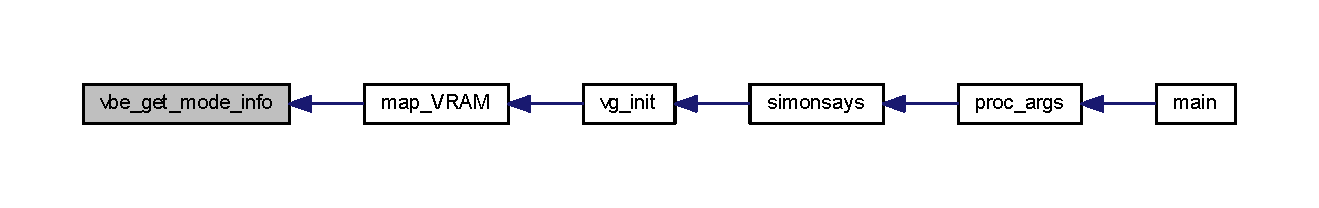
\includegraphics[width=350pt]{group__vbe_ga4ef3234e41f2050bc094a22049b69e45_icgraph}
\end{center}
\end{figure}

\hypertarget{group__video__gr}{}\section{video\+\_\+gr}
\label{group__video__gr}\index{video\+\_\+gr@{video\+\_\+gr}}
\subsection*{Functions}
\begin{DoxyCompactItemize}
\item 
void $\ast$ \hyperlink{group__video__gr_ga06d4b54021d33d2447a61b9de3982810}{map\+\_\+\+V\+R\+AM} (unsigned short mode)
\begin{DoxyCompactList}\small\item\em maps the V\+R\+AM address \end{DoxyCompactList}\item 
void $\ast$ \hyperlink{group__video__gr_gacef21667c79365d57a084bed994c2189}{vg\+\_\+init} (unsigned short mode)
\begin{DoxyCompactList}\small\item\em Initializes the video module in graphics mode. \end{DoxyCompactList}\item 
int \hyperlink{group__video__gr_ga42f593e6656f1a978315aff02b1bcebf}{vg\+\_\+exit} (void)
\begin{DoxyCompactList}\small\item\em Returns to default Minix 3 text mode (0x03\+: 25 x 80, 16 colors) \end{DoxyCompactList}\item 
unsigned \hyperlink{group__video__gr_gae2b9b38f4f97e1c580123c8e9a993353}{get\+Hor\+Resolution} ()
\begin{DoxyCompactList}\small\item\em Gives the current video horizontal resolution. \end{DoxyCompactList}\item 
unsigned \hyperlink{group__video__gr_ga7ee85b0f333d227380a2c43e5fb8507a}{get\+Ver\+Resolution} ()
\begin{DoxyCompactList}\small\item\em Gives the current video vertical resolution. \end{DoxyCompactList}\item 
char $\ast$ \hyperlink{group__video__gr_ga0823d182cf2b320e5f344bdc420a02d0}{get\+Graphics\+Buffer} ()
\begin{DoxyCompactList}\small\item\em Gives the double buffer\textquotesingle{}s address. \end{DoxyCompactList}\item 
void \hyperlink{group__video__gr_gad42c7cf5f54fed0714fcf1f6e5e35bee}{swap\+\_\+buffer} ()
\begin{DoxyCompactList}\small\item\em Sends the double buffer content to the V\+R\+AM. \end{DoxyCompactList}\end{DoxyCompactItemize}


\subsection{Detailed Description}
Functions for outputing data to screen in graphics mode 

\subsection{Function Documentation}
\mbox{\Hypertarget{group__video__gr_ga0823d182cf2b320e5f344bdc420a02d0}\label{group__video__gr_ga0823d182cf2b320e5f344bdc420a02d0}} 
\index{video\+\_\+gr@{video\+\_\+gr}!get\+Graphics\+Buffer@{get\+Graphics\+Buffer}}
\index{get\+Graphics\+Buffer@{get\+Graphics\+Buffer}!video\+\_\+gr@{video\+\_\+gr}}
\subsubsection{\texorpdfstring{get\+Graphics\+Buffer()}{getGraphicsBuffer()}}
{\footnotesize\ttfamily char$\ast$ get\+Graphics\+Buffer (\begin{DoxyParamCaption}{ }\end{DoxyParamCaption})}



Gives the double buffer\textquotesingle{}s address. 

\begin{DoxyReturn}{Returns}
double buffer\textquotesingle{}s address 
\end{DoxyReturn}
Here is the caller graph for this function\+:\nopagebreak
\begin{figure}[H]
\begin{center}
\leavevmode
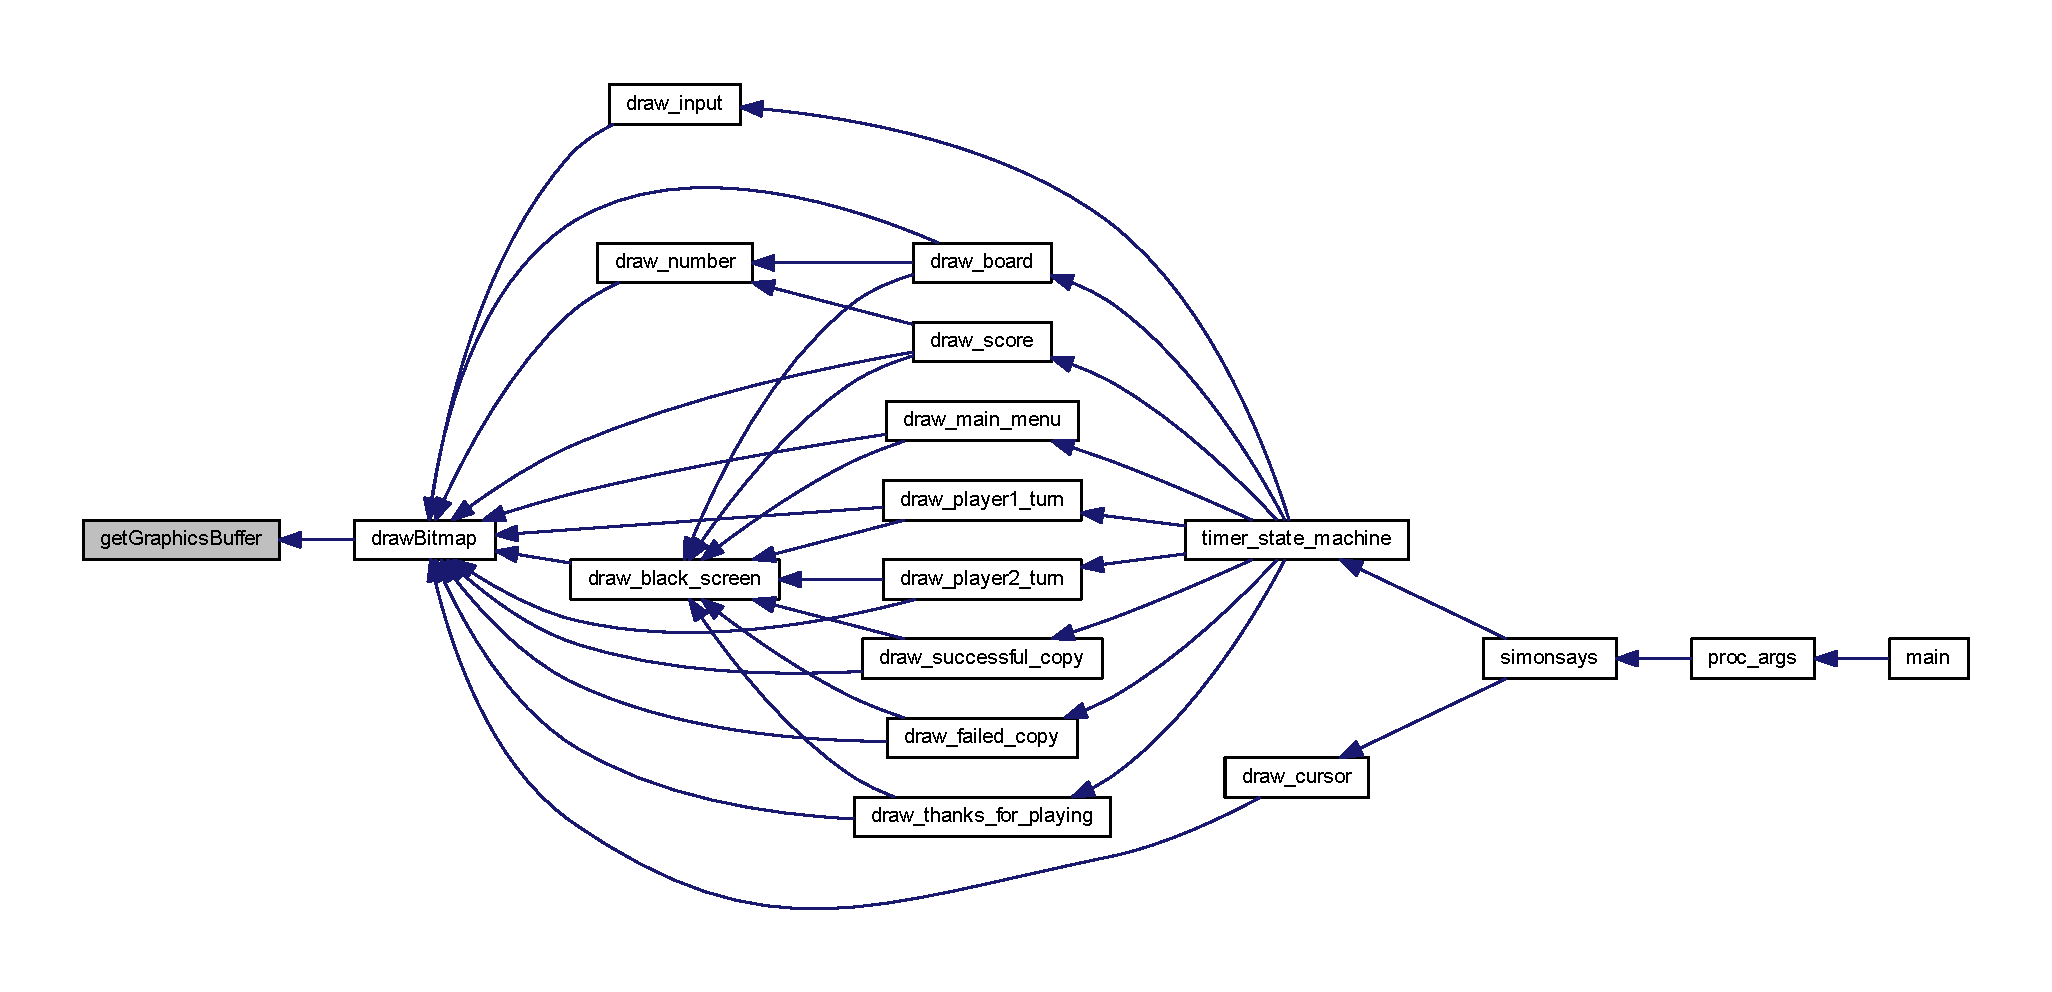
\includegraphics[width=350pt]{group__video__gr_ga0823d182cf2b320e5f344bdc420a02d0_icgraph}
\end{center}
\end{figure}
\mbox{\Hypertarget{group__video__gr_gae2b9b38f4f97e1c580123c8e9a993353}\label{group__video__gr_gae2b9b38f4f97e1c580123c8e9a993353}} 
\index{video\+\_\+gr@{video\+\_\+gr}!get\+Hor\+Resolution@{get\+Hor\+Resolution}}
\index{get\+Hor\+Resolution@{get\+Hor\+Resolution}!video\+\_\+gr@{video\+\_\+gr}}
\subsubsection{\texorpdfstring{get\+Hor\+Resolution()}{getHorResolution()}}
{\footnotesize\ttfamily unsigned get\+Hor\+Resolution (\begin{DoxyParamCaption}{ }\end{DoxyParamCaption})}



Gives the current video horizontal resolution. 

\begin{DoxyReturn}{Returns}
current video horizontal resolution 
\end{DoxyReturn}
Here is the caller graph for this function\+:\nopagebreak
\begin{figure}[H]
\begin{center}
\leavevmode
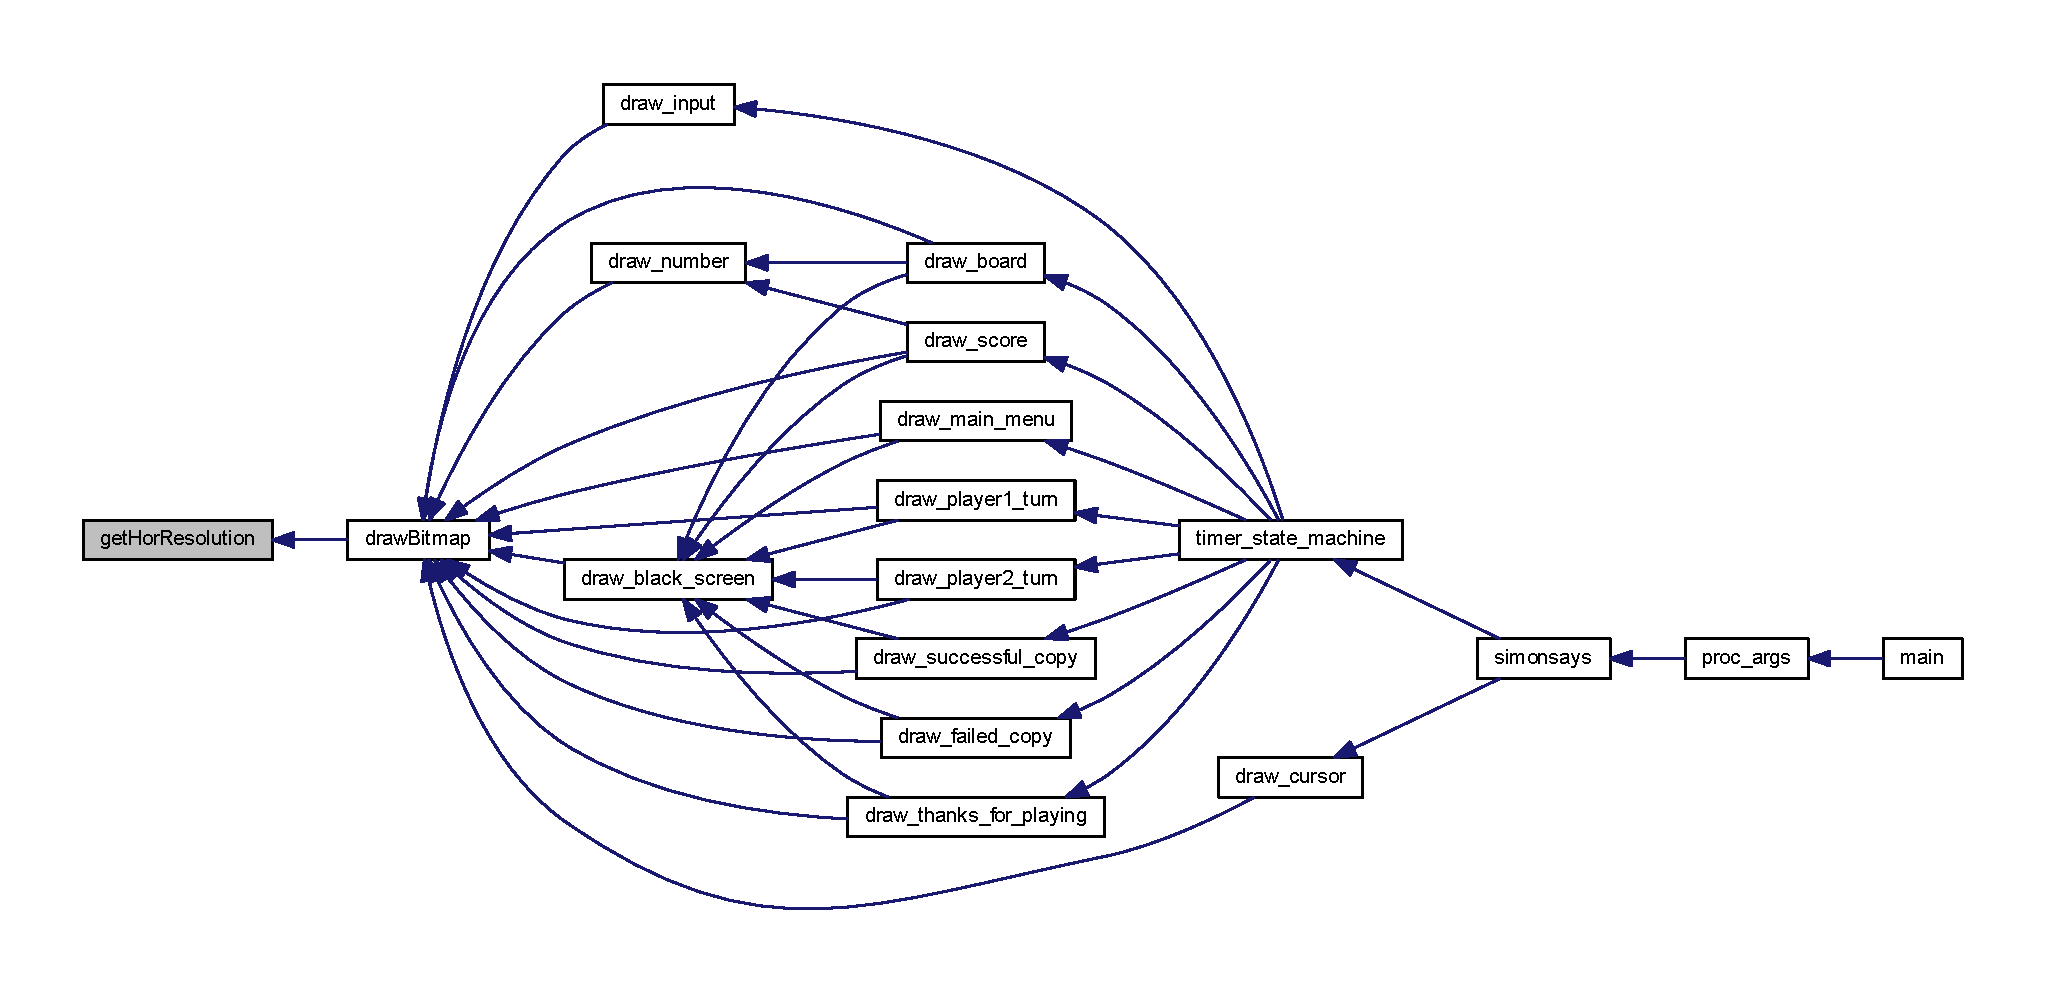
\includegraphics[width=350pt]{group__video__gr_gae2b9b38f4f97e1c580123c8e9a993353_icgraph}
\end{center}
\end{figure}
\mbox{\Hypertarget{group__video__gr_ga7ee85b0f333d227380a2c43e5fb8507a}\label{group__video__gr_ga7ee85b0f333d227380a2c43e5fb8507a}} 
\index{video\+\_\+gr@{video\+\_\+gr}!get\+Ver\+Resolution@{get\+Ver\+Resolution}}
\index{get\+Ver\+Resolution@{get\+Ver\+Resolution}!video\+\_\+gr@{video\+\_\+gr}}
\subsubsection{\texorpdfstring{get\+Ver\+Resolution()}{getVerResolution()}}
{\footnotesize\ttfamily unsigned get\+Ver\+Resolution (\begin{DoxyParamCaption}{ }\end{DoxyParamCaption})}



Gives the current video vertical resolution. 

\begin{DoxyReturn}{Returns}
current video vertical resolution 
\end{DoxyReturn}
Here is the caller graph for this function\+:\nopagebreak
\begin{figure}[H]
\begin{center}
\leavevmode
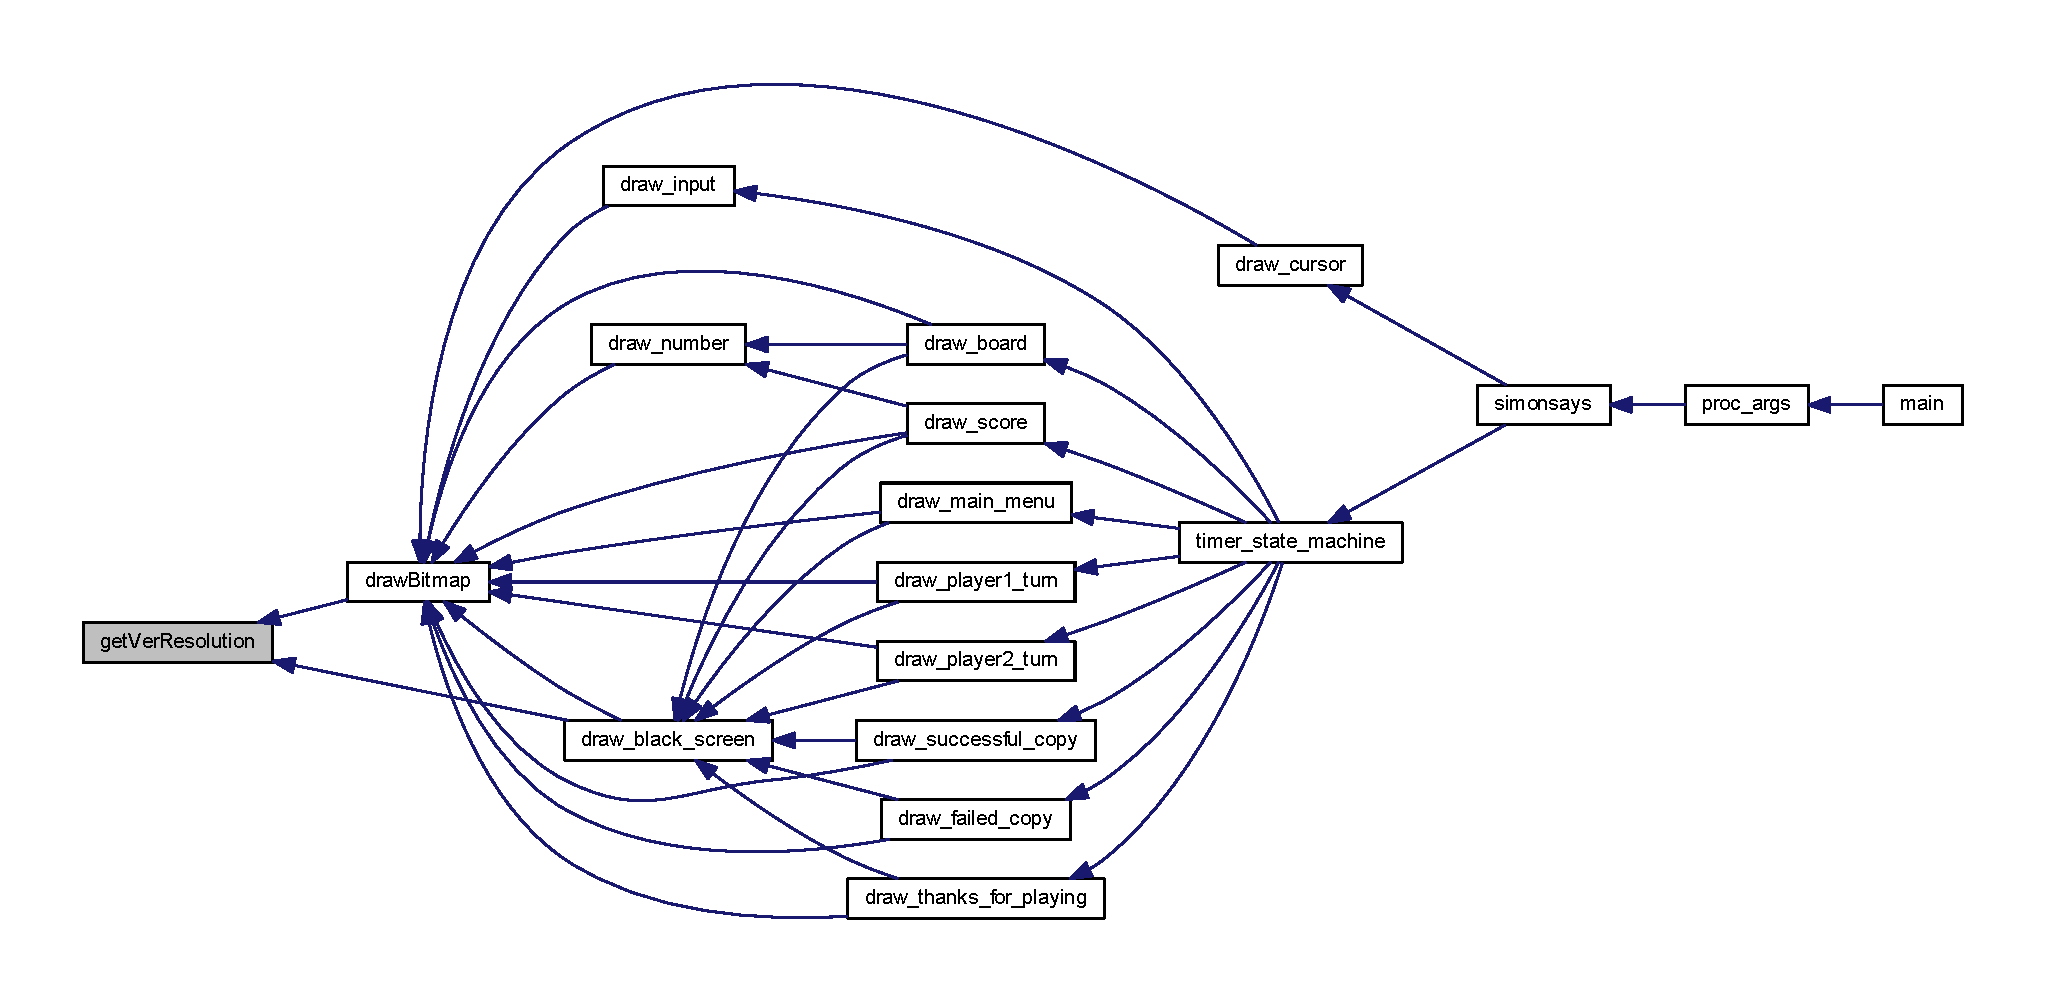
\includegraphics[width=350pt]{group__video__gr_ga7ee85b0f333d227380a2c43e5fb8507a_icgraph}
\end{center}
\end{figure}
\mbox{\Hypertarget{group__video__gr_ga06d4b54021d33d2447a61b9de3982810}\label{group__video__gr_ga06d4b54021d33d2447a61b9de3982810}} 
\index{video\+\_\+gr@{video\+\_\+gr}!map\+\_\+\+V\+R\+AM@{map\+\_\+\+V\+R\+AM}}
\index{map\+\_\+\+V\+R\+AM@{map\+\_\+\+V\+R\+AM}!video\+\_\+gr@{video\+\_\+gr}}
\subsubsection{\texorpdfstring{map\+\_\+\+V\+R\+A\+M()}{map\_VRAM()}}
{\footnotesize\ttfamily void$\ast$ map\+\_\+\+V\+R\+AM (\begin{DoxyParamCaption}\item[{unsigned short}]{mode }\end{DoxyParamCaption})}



maps the V\+R\+AM address 


\begin{DoxyParams}{Parameters}
{\em mode} & video mode to wich the graphics will be set \\
\hline
\end{DoxyParams}
Here is the call graph for this function\+:\nopagebreak
\begin{figure}[H]
\begin{center}
\leavevmode
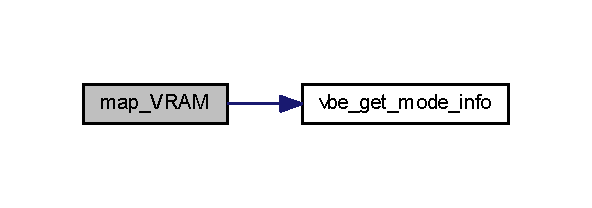
\includegraphics[width=284pt]{group__video__gr_ga06d4b54021d33d2447a61b9de3982810_cgraph}
\end{center}
\end{figure}
Here is the caller graph for this function\+:\nopagebreak
\begin{figure}[H]
\begin{center}
\leavevmode
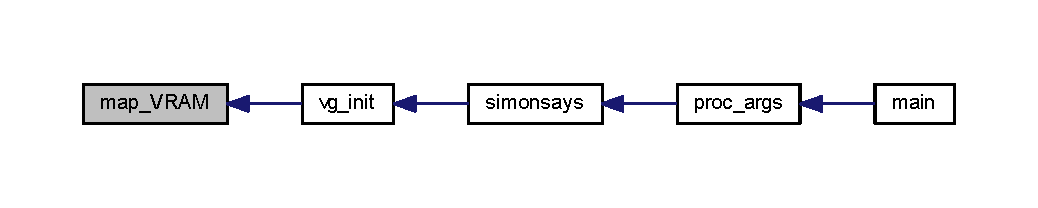
\includegraphics[width=350pt]{group__video__gr_ga06d4b54021d33d2447a61b9de3982810_icgraph}
\end{center}
\end{figure}
\mbox{\Hypertarget{group__video__gr_gad42c7cf5f54fed0714fcf1f6e5e35bee}\label{group__video__gr_gad42c7cf5f54fed0714fcf1f6e5e35bee}} 
\index{video\+\_\+gr@{video\+\_\+gr}!swap\+\_\+buffer@{swap\+\_\+buffer}}
\index{swap\+\_\+buffer@{swap\+\_\+buffer}!video\+\_\+gr@{video\+\_\+gr}}
\subsubsection{\texorpdfstring{swap\+\_\+buffer()}{swap\_buffer()}}
{\footnotesize\ttfamily void swap\+\_\+buffer (\begin{DoxyParamCaption}{ }\end{DoxyParamCaption})}



Sends the double buffer content to the V\+R\+AM. 

Here is the caller graph for this function\+:\nopagebreak
\begin{figure}[H]
\begin{center}
\leavevmode
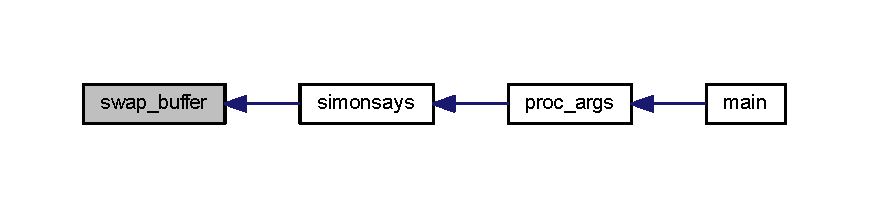
\includegraphics[width=350pt]{group__video__gr_gad42c7cf5f54fed0714fcf1f6e5e35bee_icgraph}
\end{center}
\end{figure}
\mbox{\Hypertarget{group__video__gr_ga42f593e6656f1a978315aff02b1bcebf}\label{group__video__gr_ga42f593e6656f1a978315aff02b1bcebf}} 
\index{video\+\_\+gr@{video\+\_\+gr}!vg\+\_\+exit@{vg\+\_\+exit}}
\index{vg\+\_\+exit@{vg\+\_\+exit}!video\+\_\+gr@{video\+\_\+gr}}
\subsubsection{\texorpdfstring{vg\+\_\+exit()}{vg\_exit()}}
{\footnotesize\ttfamily int vg\+\_\+exit (\begin{DoxyParamCaption}\item[{void}]{ }\end{DoxyParamCaption})}



Returns to default Minix 3 text mode (0x03\+: 25 x 80, 16 colors) 

\begin{DoxyReturn}{Returns}
0 upon success, non-\/zero upon failure 
\end{DoxyReturn}
Here is the caller graph for this function\+:\nopagebreak
\begin{figure}[H]
\begin{center}
\leavevmode
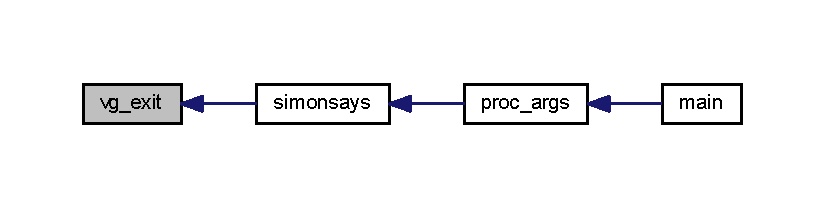
\includegraphics[width=350pt]{group__video__gr_ga42f593e6656f1a978315aff02b1bcebf_icgraph}
\end{center}
\end{figure}
\mbox{\Hypertarget{group__video__gr_gacef21667c79365d57a084bed994c2189}\label{group__video__gr_gacef21667c79365d57a084bed994c2189}} 
\index{video\+\_\+gr@{video\+\_\+gr}!vg\+\_\+init@{vg\+\_\+init}}
\index{vg\+\_\+init@{vg\+\_\+init}!video\+\_\+gr@{video\+\_\+gr}}
\subsubsection{\texorpdfstring{vg\+\_\+init()}{vg\_init()}}
{\footnotesize\ttfamily void$\ast$ vg\+\_\+init (\begin{DoxyParamCaption}\item[{unsigned short}]{mode }\end{DoxyParamCaption})}



Initializes the video module in graphics mode. 

Uses the V\+BE I\+NT 0x10 interface to set the desired graphics mode, maps V\+R\+AM to the process\textquotesingle{} address space and initializes static global variables with the resolution of the screen, and the number of colors


\begin{DoxyParams}{Parameters}
{\em mode} & 16-\/bit V\+BE mode to set \\
\hline
\end{DoxyParams}
\begin{DoxyReturn}{Returns}
Virtual address V\+R\+AM was mapped to. N\+U\+LL, upon failure. 
\end{DoxyReturn}
Here is the call graph for this function\+:\nopagebreak
\begin{figure}[H]
\begin{center}
\leavevmode
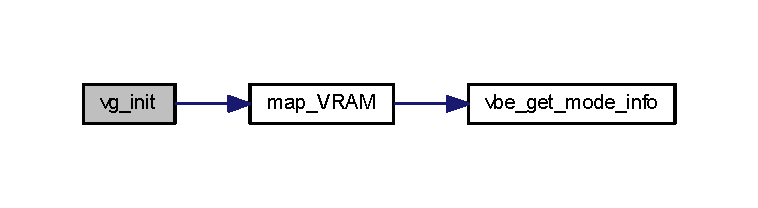
\includegraphics[width=350pt]{group__video__gr_gacef21667c79365d57a084bed994c2189_cgraph}
\end{center}
\end{figure}
Here is the caller graph for this function\+:\nopagebreak
\begin{figure}[H]
\begin{center}
\leavevmode
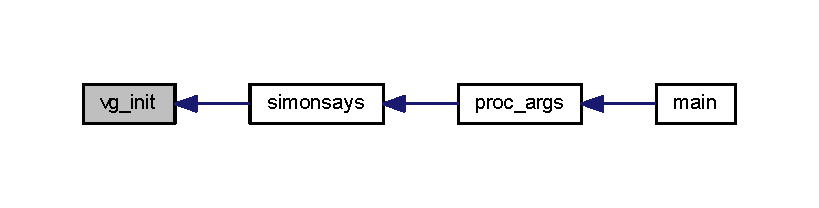
\includegraphics[width=350pt]{group__video__gr_gacef21667c79365d57a084bed994c2189_icgraph}
\end{center}
\end{figure}

\chapter{Data Structure Documentation}
\hypertarget{struct____attribute____}{}\section{\+\_\+\+\_\+attribute\+\_\+\+\_\+ Struct Reference}
\label{struct____attribute____}\index{\+\_\+\+\_\+attribute\+\_\+\+\_\+@{\+\_\+\+\_\+attribute\+\_\+\+\_\+}}


{\ttfamily \#include $<$vbe.\+h$>$}

\subsection*{Data Fields}
\begin{DoxyCompactItemize}
\item 
uint16\+\_\+t \hyperlink{struct____attribute_____ad7593abf9d201ce5e59de60baba548cd}{Mode\+Attributes}
\begin{DoxyCompactList}\small\item\em mode attributes \end{DoxyCompactList}\item 
uint8\+\_\+t \hyperlink{struct____attribute_____aaa90049ea7f03763acbbf75240f4f5d8}{Win\+A\+Attributes}
\begin{DoxyCompactList}\small\item\em window A attributes \end{DoxyCompactList}\item 
uint8\+\_\+t \hyperlink{struct____attribute_____a370ddeb84e904ef1000fe57905ebf6b8}{Win\+B\+Attributes}
\begin{DoxyCompactList}\small\item\em window B attributes \end{DoxyCompactList}\item 
uint16\+\_\+t \hyperlink{struct____attribute_____a38f205f799c6929629395f03e24de077}{Win\+Granularity}
\begin{DoxyCompactList}\small\item\em window granularity \end{DoxyCompactList}\item 
uint16\+\_\+t \hyperlink{struct____attribute_____a78985f1c5ae166cb560099273cc558b4}{Win\+Size}
\begin{DoxyCompactList}\small\item\em window size \end{DoxyCompactList}\item 
uint16\+\_\+t \hyperlink{struct____attribute_____a99b747099fd4d4271b0f0bc29f31c48f}{Win\+A\+Segment}
\begin{DoxyCompactList}\small\item\em window A start segment \end{DoxyCompactList}\item 
uint16\+\_\+t \hyperlink{struct____attribute_____a9edf422a931df7c7a1d5f82afb911566}{Win\+B\+Segment}
\begin{DoxyCompactList}\small\item\em window B start segment \end{DoxyCompactList}\item 
phys\+\_\+bytes \hyperlink{struct____attribute_____affd250a4766543099f253e27af3abc35}{Win\+Func\+Ptr}
\begin{DoxyCompactList}\small\item\em real mode/far pointer to window function \end{DoxyCompactList}\item 
uint16\+\_\+t \hyperlink{struct____attribute_____afe40654a51bf4a12a8b376ff3506688e}{Bytes\+Per\+Scan\+Line}
\begin{DoxyCompactList}\small\item\em bytes per scan line \end{DoxyCompactList}\item 
uint16\+\_\+t \hyperlink{struct____attribute_____a16f6408e5a85c7a7785a0cee64b6a219}{X\+Resolution}
\begin{DoxyCompactList}\small\item\em horizontal resolution in pixels/characters \end{DoxyCompactList}\item 
uint16\+\_\+t \hyperlink{struct____attribute_____afa8aba2156994750d500f85d0f8425cb}{Y\+Resolution}
\begin{DoxyCompactList}\small\item\em vertical resolution in pixels/characters \end{DoxyCompactList}\item 
uint8\+\_\+t \hyperlink{struct____attribute_____a047d8f41434f02589d0c9b90b17c67eb}{X\+Char\+Size}
\begin{DoxyCompactList}\small\item\em character cell width in pixels \end{DoxyCompactList}\item 
uint8\+\_\+t \hyperlink{struct____attribute_____a330f00ebd49dccd2325d43cdbd646f09}{Y\+Char\+Size}
\begin{DoxyCompactList}\small\item\em character cell height in pixels \end{DoxyCompactList}\item 
uint8\+\_\+t \hyperlink{struct____attribute_____a51268efaac55d78e17263aff9a447998}{Number\+Of\+Planes}
\begin{DoxyCompactList}\small\item\em number of memory planes \end{DoxyCompactList}\item 
uint8\+\_\+t \hyperlink{struct____attribute_____a03756ae144fce823087a2a4255bf4bb1}{Bits\+Per\+Pixel}
\begin{DoxyCompactList}\small\item\em bits per pixel \end{DoxyCompactList}\item 
uint8\+\_\+t \hyperlink{struct____attribute_____aa955c03441b6d3e55b2ba4be4dae56a2}{Number\+Of\+Banks}
\begin{DoxyCompactList}\small\item\em number of banks \end{DoxyCompactList}\item 
uint8\+\_\+t \hyperlink{struct____attribute_____ab9be703b2b515ba3428ed97af9bb084d}{Memory\+Model}
\begin{DoxyCompactList}\small\item\em memory model type \end{DoxyCompactList}\item 
uint8\+\_\+t \hyperlink{struct____attribute_____a7e31ea09e6e6755e3a504b9c76b3f545}{Bank\+Size}
\begin{DoxyCompactList}\small\item\em bank size in KB \end{DoxyCompactList}\item 
uint8\+\_\+t \hyperlink{struct____attribute_____a7033bb4cac6dc49f68ca4df855151e09}{Number\+Of\+Image\+Pages}
\begin{DoxyCompactList}\small\item\em number of images \end{DoxyCompactList}\item 
uint8\+\_\+t \hyperlink{struct____attribute_____a604037992fe7e5fd08e1bcc684a1b12d}{Reserved1}
\begin{DoxyCompactList}\small\item\em reserved for page function \end{DoxyCompactList}\item 
uint8\+\_\+t \hyperlink{struct____attribute_____a5e25f6a8eedde631fff577bcf7d4f6f4}{Red\+Mask\+Size}
\item 
uint8\+\_\+t \hyperlink{struct____attribute_____a20cb142b8c1b0a2b41244fef469a11f4}{Red\+Field\+Position}
\item 
uint8\+\_\+t \hyperlink{struct____attribute_____ac7b4df72e505b74493e7d5144cbac743}{Green\+Mask\+Size}
\item 
uint8\+\_\+t \hyperlink{struct____attribute_____a602b28f8e5da781eabfd736743a6ea09}{Green\+Field\+Position}
\item 
uint8\+\_\+t \hyperlink{struct____attribute_____a84842a6a42e881ce7be87482122bcc4e}{Blue\+Mask\+Size}
\item 
uint8\+\_\+t \hyperlink{struct____attribute_____a4d0396c07a4f07556332fec2b4a6c2bf}{Blue\+Field\+Position}
\item 
uint8\+\_\+t \hyperlink{struct____attribute_____a87d544680f1132f30b038c0ebf0b829b}{Rsvd\+Mask\+Size}
\item 
uint8\+\_\+t \hyperlink{struct____attribute_____aa357b085181776f2918a6df25c88846b}{Rsvd\+Field\+Position}
\item 
uint8\+\_\+t \hyperlink{struct____attribute_____a3bf2fd2394ec8649ec3d26104be35dd7}{Direct\+Color\+Mode\+Info}
\item 
phys\+\_\+bytes \hyperlink{struct____attribute_____a1d11f4921094db253fc2c2ee6fbb2afb}{Phys\+Base\+Ptr}
\begin{DoxyCompactList}\small\item\em physical address for flat memory frame buffer \end{DoxyCompactList}\item 
uint8\+\_\+t \hyperlink{struct____attribute_____a09b5824ec5c67bee2a4b36c0ab5181bc}{Reserved2} \mbox{[}4\mbox{]}
\begin{DoxyCompactList}\small\item\em Reserved -\/ always set to 0. \end{DoxyCompactList}\item 
uint8\+\_\+t \hyperlink{struct____attribute_____a2455a82e0d8cc0e8d76e8cf77a68bd39}{Reserved3} \mbox{[}2\mbox{]}
\begin{DoxyCompactList}\small\item\em Reserved -\/ always set to 0. \end{DoxyCompactList}\item 
uint16\+\_\+t \hyperlink{struct____attribute_____a53c5060b6ac14a7418ca8421edfb9981}{Lin\+Bytes\+Per\+Scan\+Line}
\item 
uint8\+\_\+t \hyperlink{struct____attribute_____a33ba903e149724b1bc99b3b8e43a7cbe}{Bnk\+Number\+Of\+Image\+Pages}
\item 
uint8\+\_\+t \hyperlink{struct____attribute_____a3fa2352e69836f4b69b3a344ae761ba8}{Lin\+Number\+Of\+Image\+Pages}
\item 
uint8\+\_\+t \hyperlink{struct____attribute_____a1fbcef2402fe6ce7f6c006bd50eaa6da}{Lin\+Red\+Mask\+Size}
\item 
uint8\+\_\+t \hyperlink{struct____attribute_____aff962b58f86a77f12b412d47125a4993}{Lin\+Red\+Field\+Position}
\item 
uint8\+\_\+t \hyperlink{struct____attribute_____af235e505028771ab2fb84778f4dfb476}{Lin\+Green\+Mask\+Size}
\item 
uint8\+\_\+t \hyperlink{struct____attribute_____a6683a63711dbc5dfb9a2a59c55deecd5}{Lin\+Green\+Field\+Position}
\item 
uint8\+\_\+t \hyperlink{struct____attribute_____ad8a25cec803bf91fb40a20a0aa5d5bf7}{Lin\+Blue\+Mask\+Size}
\item 
uint8\+\_\+t \hyperlink{struct____attribute_____a3f38d6becbe961786cd7ab58ec37fc07}{Lin\+Blue\+Field\+Position}
\item 
uint8\+\_\+t \hyperlink{struct____attribute_____a334886fc9a915ff91966c3aac1da586a}{Lin\+Rsvd\+Mask\+Size}
\item 
uint8\+\_\+t \hyperlink{struct____attribute_____a3df070e698b5f54814e20c8813f7bf7e}{Lin\+Rsvd\+Field\+Position}
\item 
uint32\+\_\+t \hyperlink{struct____attribute_____ab1fbd72846963ebb34a308a7edf7bbe1}{Max\+Pixel\+Clock}
\item 
uint8\+\_\+t \hyperlink{struct____attribute_____a2e13c4795a00241b919aa3aab86560ce}{Reserved4} \mbox{[}190\mbox{]}
\item 
uint8\+\_\+t \hyperlink{struct____attribute_____a6b319b7f1d18ea66e69de3a573c60b15}{Vbe\+Signature}
\item 
uint16\+\_\+t \hyperlink{struct____attribute_____a7b9fef89774326b46f9481cbd9a397d3}{Vbe\+Version}
\item 
phys\+\_\+bytes \hyperlink{struct____attribute_____a20ab55e9dda8d437875255529c1cffe8}{Oem\+String\+Ptr}
\item 
uint8\+\_\+t \hyperlink{struct____attribute_____a2ee0214fbaf7a7da7462f1e270d16f6d}{Capabilities}
\item 
phys\+\_\+bytes \hyperlink{struct____attribute_____a9d989fdbcdad6a40c10fc28c0f9af760}{Video\+Mode\+Ptr}
\item 
uint16\+\_\+t \hyperlink{struct____attribute_____a3e7b41e709394a10b3667e7f27f1aa7a}{Total\+Memory}
\item 
uint16\+\_\+t \hyperlink{struct____attribute_____a133984a56ec19abf4fcb2e6ae71d6498}{Oem\+Software\+Rev}
\item 
phys\+\_\+bytes \hyperlink{struct____attribute_____affd3a330afde841405f89bbcd05af4f0}{Oem\+Vendor\+Name\+Ptr}
\item 
phys\+\_\+bytes \hyperlink{struct____attribute_____afd3d28c2078a683b1ed64ea21905fcfe}{Oem\+Product\+Name\+Ptr}
\item 
phys\+\_\+bytes \hyperlink{struct____attribute_____a239cba41d0489da5b79556b45797c6b0}{Oem\+Product\+Rev\+Ptr}
\item 
uint8\+\_\+t \hyperlink{struct____attribute_____a2c3b1cbb6bad5c51d4be4e57255a61d2}{Reserved} \mbox{[}222\mbox{]}
\item 
uint8\+\_\+t \hyperlink{struct____attribute_____a966ae75c33c2d65b4f0c916f093acac0}{Oem\+Data} \mbox{[}256\mbox{]}
\end{DoxyCompactItemize}


\subsection{Field Documentation}
\mbox{\Hypertarget{struct____attribute_____a7e31ea09e6e6755e3a504b9c76b3f545}\label{struct____attribute_____a7e31ea09e6e6755e3a504b9c76b3f545}} 
\index{\+\_\+\+\_\+attribute\+\_\+\+\_\+@{\+\_\+\+\_\+attribute\+\_\+\+\_\+}!Bank\+Size@{Bank\+Size}}
\index{Bank\+Size@{Bank\+Size}!\+\_\+\+\_\+attribute\+\_\+\+\_\+@{\+\_\+\+\_\+attribute\+\_\+\+\_\+}}
\subsubsection{\texorpdfstring{Bank\+Size}{BankSize}}
{\footnotesize\ttfamily uint8\+\_\+t Bank\+Size}



bank size in KB 

\mbox{\Hypertarget{struct____attribute_____a03756ae144fce823087a2a4255bf4bb1}\label{struct____attribute_____a03756ae144fce823087a2a4255bf4bb1}} 
\index{\+\_\+\+\_\+attribute\+\_\+\+\_\+@{\+\_\+\+\_\+attribute\+\_\+\+\_\+}!Bits\+Per\+Pixel@{Bits\+Per\+Pixel}}
\index{Bits\+Per\+Pixel@{Bits\+Per\+Pixel}!\+\_\+\+\_\+attribute\+\_\+\+\_\+@{\+\_\+\+\_\+attribute\+\_\+\+\_\+}}
\subsubsection{\texorpdfstring{Bits\+Per\+Pixel}{BitsPerPixel}}
{\footnotesize\ttfamily uint8\+\_\+t Bits\+Per\+Pixel}



bits per pixel 

\mbox{\Hypertarget{struct____attribute_____a4d0396c07a4f07556332fec2b4a6c2bf}\label{struct____attribute_____a4d0396c07a4f07556332fec2b4a6c2bf}} 
\index{\+\_\+\+\_\+attribute\+\_\+\+\_\+@{\+\_\+\+\_\+attribute\+\_\+\+\_\+}!Blue\+Field\+Position@{Blue\+Field\+Position}}
\index{Blue\+Field\+Position@{Blue\+Field\+Position}!\+\_\+\+\_\+attribute\+\_\+\+\_\+@{\+\_\+\+\_\+attribute\+\_\+\+\_\+}}
\subsubsection{\texorpdfstring{Blue\+Field\+Position}{BlueFieldPosition}}
{\footnotesize\ttfamily uint8\+\_\+t Blue\+Field\+Position}

\mbox{\Hypertarget{struct____attribute_____a84842a6a42e881ce7be87482122bcc4e}\label{struct____attribute_____a84842a6a42e881ce7be87482122bcc4e}} 
\index{\+\_\+\+\_\+attribute\+\_\+\+\_\+@{\+\_\+\+\_\+attribute\+\_\+\+\_\+}!Blue\+Mask\+Size@{Blue\+Mask\+Size}}
\index{Blue\+Mask\+Size@{Blue\+Mask\+Size}!\+\_\+\+\_\+attribute\+\_\+\+\_\+@{\+\_\+\+\_\+attribute\+\_\+\+\_\+}}
\subsubsection{\texorpdfstring{Blue\+Mask\+Size}{BlueMaskSize}}
{\footnotesize\ttfamily uint8\+\_\+t Blue\+Mask\+Size}

\mbox{\Hypertarget{struct____attribute_____a33ba903e149724b1bc99b3b8e43a7cbe}\label{struct____attribute_____a33ba903e149724b1bc99b3b8e43a7cbe}} 
\index{\+\_\+\+\_\+attribute\+\_\+\+\_\+@{\+\_\+\+\_\+attribute\+\_\+\+\_\+}!Bnk\+Number\+Of\+Image\+Pages@{Bnk\+Number\+Of\+Image\+Pages}}
\index{Bnk\+Number\+Of\+Image\+Pages@{Bnk\+Number\+Of\+Image\+Pages}!\+\_\+\+\_\+attribute\+\_\+\+\_\+@{\+\_\+\+\_\+attribute\+\_\+\+\_\+}}
\subsubsection{\texorpdfstring{Bnk\+Number\+Of\+Image\+Pages}{BnkNumberOfImagePages}}
{\footnotesize\ttfamily uint8\+\_\+t Bnk\+Number\+Of\+Image\+Pages}

\mbox{\Hypertarget{struct____attribute_____afe40654a51bf4a12a8b376ff3506688e}\label{struct____attribute_____afe40654a51bf4a12a8b376ff3506688e}} 
\index{\+\_\+\+\_\+attribute\+\_\+\+\_\+@{\+\_\+\+\_\+attribute\+\_\+\+\_\+}!Bytes\+Per\+Scan\+Line@{Bytes\+Per\+Scan\+Line}}
\index{Bytes\+Per\+Scan\+Line@{Bytes\+Per\+Scan\+Line}!\+\_\+\+\_\+attribute\+\_\+\+\_\+@{\+\_\+\+\_\+attribute\+\_\+\+\_\+}}
\subsubsection{\texorpdfstring{Bytes\+Per\+Scan\+Line}{BytesPerScanLine}}
{\footnotesize\ttfamily uint16\+\_\+t Bytes\+Per\+Scan\+Line}



bytes per scan line 

\mbox{\Hypertarget{struct____attribute_____a2ee0214fbaf7a7da7462f1e270d16f6d}\label{struct____attribute_____a2ee0214fbaf7a7da7462f1e270d16f6d}} 
\index{\+\_\+\+\_\+attribute\+\_\+\+\_\+@{\+\_\+\+\_\+attribute\+\_\+\+\_\+}!Capabilities@{Capabilities}}
\index{Capabilities@{Capabilities}!\+\_\+\+\_\+attribute\+\_\+\+\_\+@{\+\_\+\+\_\+attribute\+\_\+\+\_\+}}
\subsubsection{\texorpdfstring{Capabilities}{Capabilities}}
{\footnotesize\ttfamily uint8\+\_\+t Capabilities}

\mbox{\Hypertarget{struct____attribute_____a3bf2fd2394ec8649ec3d26104be35dd7}\label{struct____attribute_____a3bf2fd2394ec8649ec3d26104be35dd7}} 
\index{\+\_\+\+\_\+attribute\+\_\+\+\_\+@{\+\_\+\+\_\+attribute\+\_\+\+\_\+}!Direct\+Color\+Mode\+Info@{Direct\+Color\+Mode\+Info}}
\index{Direct\+Color\+Mode\+Info@{Direct\+Color\+Mode\+Info}!\+\_\+\+\_\+attribute\+\_\+\+\_\+@{\+\_\+\+\_\+attribute\+\_\+\+\_\+}}
\subsubsection{\texorpdfstring{Direct\+Color\+Mode\+Info}{DirectColorModeInfo}}
{\footnotesize\ttfamily uint8\+\_\+t Direct\+Color\+Mode\+Info}

\mbox{\Hypertarget{struct____attribute_____a602b28f8e5da781eabfd736743a6ea09}\label{struct____attribute_____a602b28f8e5da781eabfd736743a6ea09}} 
\index{\+\_\+\+\_\+attribute\+\_\+\+\_\+@{\+\_\+\+\_\+attribute\+\_\+\+\_\+}!Green\+Field\+Position@{Green\+Field\+Position}}
\index{Green\+Field\+Position@{Green\+Field\+Position}!\+\_\+\+\_\+attribute\+\_\+\+\_\+@{\+\_\+\+\_\+attribute\+\_\+\+\_\+}}
\subsubsection{\texorpdfstring{Green\+Field\+Position}{GreenFieldPosition}}
{\footnotesize\ttfamily uint8\+\_\+t Green\+Field\+Position}

\mbox{\Hypertarget{struct____attribute_____ac7b4df72e505b74493e7d5144cbac743}\label{struct____attribute_____ac7b4df72e505b74493e7d5144cbac743}} 
\index{\+\_\+\+\_\+attribute\+\_\+\+\_\+@{\+\_\+\+\_\+attribute\+\_\+\+\_\+}!Green\+Mask\+Size@{Green\+Mask\+Size}}
\index{Green\+Mask\+Size@{Green\+Mask\+Size}!\+\_\+\+\_\+attribute\+\_\+\+\_\+@{\+\_\+\+\_\+attribute\+\_\+\+\_\+}}
\subsubsection{\texorpdfstring{Green\+Mask\+Size}{GreenMaskSize}}
{\footnotesize\ttfamily uint8\+\_\+t Green\+Mask\+Size}

\mbox{\Hypertarget{struct____attribute_____a3f38d6becbe961786cd7ab58ec37fc07}\label{struct____attribute_____a3f38d6becbe961786cd7ab58ec37fc07}} 
\index{\+\_\+\+\_\+attribute\+\_\+\+\_\+@{\+\_\+\+\_\+attribute\+\_\+\+\_\+}!Lin\+Blue\+Field\+Position@{Lin\+Blue\+Field\+Position}}
\index{Lin\+Blue\+Field\+Position@{Lin\+Blue\+Field\+Position}!\+\_\+\+\_\+attribute\+\_\+\+\_\+@{\+\_\+\+\_\+attribute\+\_\+\+\_\+}}
\subsubsection{\texorpdfstring{Lin\+Blue\+Field\+Position}{LinBlueFieldPosition}}
{\footnotesize\ttfamily uint8\+\_\+t Lin\+Blue\+Field\+Position}

\mbox{\Hypertarget{struct____attribute_____ad8a25cec803bf91fb40a20a0aa5d5bf7}\label{struct____attribute_____ad8a25cec803bf91fb40a20a0aa5d5bf7}} 
\index{\+\_\+\+\_\+attribute\+\_\+\+\_\+@{\+\_\+\+\_\+attribute\+\_\+\+\_\+}!Lin\+Blue\+Mask\+Size@{Lin\+Blue\+Mask\+Size}}
\index{Lin\+Blue\+Mask\+Size@{Lin\+Blue\+Mask\+Size}!\+\_\+\+\_\+attribute\+\_\+\+\_\+@{\+\_\+\+\_\+attribute\+\_\+\+\_\+}}
\subsubsection{\texorpdfstring{Lin\+Blue\+Mask\+Size}{LinBlueMaskSize}}
{\footnotesize\ttfamily uint8\+\_\+t Lin\+Blue\+Mask\+Size}

\mbox{\Hypertarget{struct____attribute_____a53c5060b6ac14a7418ca8421edfb9981}\label{struct____attribute_____a53c5060b6ac14a7418ca8421edfb9981}} 
\index{\+\_\+\+\_\+attribute\+\_\+\+\_\+@{\+\_\+\+\_\+attribute\+\_\+\+\_\+}!Lin\+Bytes\+Per\+Scan\+Line@{Lin\+Bytes\+Per\+Scan\+Line}}
\index{Lin\+Bytes\+Per\+Scan\+Line@{Lin\+Bytes\+Per\+Scan\+Line}!\+\_\+\+\_\+attribute\+\_\+\+\_\+@{\+\_\+\+\_\+attribute\+\_\+\+\_\+}}
\subsubsection{\texorpdfstring{Lin\+Bytes\+Per\+Scan\+Line}{LinBytesPerScanLine}}
{\footnotesize\ttfamily uint16\+\_\+t Lin\+Bytes\+Per\+Scan\+Line}

\mbox{\Hypertarget{struct____attribute_____a6683a63711dbc5dfb9a2a59c55deecd5}\label{struct____attribute_____a6683a63711dbc5dfb9a2a59c55deecd5}} 
\index{\+\_\+\+\_\+attribute\+\_\+\+\_\+@{\+\_\+\+\_\+attribute\+\_\+\+\_\+}!Lin\+Green\+Field\+Position@{Lin\+Green\+Field\+Position}}
\index{Lin\+Green\+Field\+Position@{Lin\+Green\+Field\+Position}!\+\_\+\+\_\+attribute\+\_\+\+\_\+@{\+\_\+\+\_\+attribute\+\_\+\+\_\+}}
\subsubsection{\texorpdfstring{Lin\+Green\+Field\+Position}{LinGreenFieldPosition}}
{\footnotesize\ttfamily uint8\+\_\+t Lin\+Green\+Field\+Position}

\mbox{\Hypertarget{struct____attribute_____af235e505028771ab2fb84778f4dfb476}\label{struct____attribute_____af235e505028771ab2fb84778f4dfb476}} 
\index{\+\_\+\+\_\+attribute\+\_\+\+\_\+@{\+\_\+\+\_\+attribute\+\_\+\+\_\+}!Lin\+Green\+Mask\+Size@{Lin\+Green\+Mask\+Size}}
\index{Lin\+Green\+Mask\+Size@{Lin\+Green\+Mask\+Size}!\+\_\+\+\_\+attribute\+\_\+\+\_\+@{\+\_\+\+\_\+attribute\+\_\+\+\_\+}}
\subsubsection{\texorpdfstring{Lin\+Green\+Mask\+Size}{LinGreenMaskSize}}
{\footnotesize\ttfamily uint8\+\_\+t Lin\+Green\+Mask\+Size}

\mbox{\Hypertarget{struct____attribute_____a3fa2352e69836f4b69b3a344ae761ba8}\label{struct____attribute_____a3fa2352e69836f4b69b3a344ae761ba8}} 
\index{\+\_\+\+\_\+attribute\+\_\+\+\_\+@{\+\_\+\+\_\+attribute\+\_\+\+\_\+}!Lin\+Number\+Of\+Image\+Pages@{Lin\+Number\+Of\+Image\+Pages}}
\index{Lin\+Number\+Of\+Image\+Pages@{Lin\+Number\+Of\+Image\+Pages}!\+\_\+\+\_\+attribute\+\_\+\+\_\+@{\+\_\+\+\_\+attribute\+\_\+\+\_\+}}
\subsubsection{\texorpdfstring{Lin\+Number\+Of\+Image\+Pages}{LinNumberOfImagePages}}
{\footnotesize\ttfamily uint8\+\_\+t Lin\+Number\+Of\+Image\+Pages}

\mbox{\Hypertarget{struct____attribute_____aff962b58f86a77f12b412d47125a4993}\label{struct____attribute_____aff962b58f86a77f12b412d47125a4993}} 
\index{\+\_\+\+\_\+attribute\+\_\+\+\_\+@{\+\_\+\+\_\+attribute\+\_\+\+\_\+}!Lin\+Red\+Field\+Position@{Lin\+Red\+Field\+Position}}
\index{Lin\+Red\+Field\+Position@{Lin\+Red\+Field\+Position}!\+\_\+\+\_\+attribute\+\_\+\+\_\+@{\+\_\+\+\_\+attribute\+\_\+\+\_\+}}
\subsubsection{\texorpdfstring{Lin\+Red\+Field\+Position}{LinRedFieldPosition}}
{\footnotesize\ttfamily uint8\+\_\+t Lin\+Red\+Field\+Position}

\mbox{\Hypertarget{struct____attribute_____a1fbcef2402fe6ce7f6c006bd50eaa6da}\label{struct____attribute_____a1fbcef2402fe6ce7f6c006bd50eaa6da}} 
\index{\+\_\+\+\_\+attribute\+\_\+\+\_\+@{\+\_\+\+\_\+attribute\+\_\+\+\_\+}!Lin\+Red\+Mask\+Size@{Lin\+Red\+Mask\+Size}}
\index{Lin\+Red\+Mask\+Size@{Lin\+Red\+Mask\+Size}!\+\_\+\+\_\+attribute\+\_\+\+\_\+@{\+\_\+\+\_\+attribute\+\_\+\+\_\+}}
\subsubsection{\texorpdfstring{Lin\+Red\+Mask\+Size}{LinRedMaskSize}}
{\footnotesize\ttfamily uint8\+\_\+t Lin\+Red\+Mask\+Size}

\mbox{\Hypertarget{struct____attribute_____a3df070e698b5f54814e20c8813f7bf7e}\label{struct____attribute_____a3df070e698b5f54814e20c8813f7bf7e}} 
\index{\+\_\+\+\_\+attribute\+\_\+\+\_\+@{\+\_\+\+\_\+attribute\+\_\+\+\_\+}!Lin\+Rsvd\+Field\+Position@{Lin\+Rsvd\+Field\+Position}}
\index{Lin\+Rsvd\+Field\+Position@{Lin\+Rsvd\+Field\+Position}!\+\_\+\+\_\+attribute\+\_\+\+\_\+@{\+\_\+\+\_\+attribute\+\_\+\+\_\+}}
\subsubsection{\texorpdfstring{Lin\+Rsvd\+Field\+Position}{LinRsvdFieldPosition}}
{\footnotesize\ttfamily uint8\+\_\+t Lin\+Rsvd\+Field\+Position}

\mbox{\Hypertarget{struct____attribute_____a334886fc9a915ff91966c3aac1da586a}\label{struct____attribute_____a334886fc9a915ff91966c3aac1da586a}} 
\index{\+\_\+\+\_\+attribute\+\_\+\+\_\+@{\+\_\+\+\_\+attribute\+\_\+\+\_\+}!Lin\+Rsvd\+Mask\+Size@{Lin\+Rsvd\+Mask\+Size}}
\index{Lin\+Rsvd\+Mask\+Size@{Lin\+Rsvd\+Mask\+Size}!\+\_\+\+\_\+attribute\+\_\+\+\_\+@{\+\_\+\+\_\+attribute\+\_\+\+\_\+}}
\subsubsection{\texorpdfstring{Lin\+Rsvd\+Mask\+Size}{LinRsvdMaskSize}}
{\footnotesize\ttfamily uint8\+\_\+t Lin\+Rsvd\+Mask\+Size}

\mbox{\Hypertarget{struct____attribute_____ab1fbd72846963ebb34a308a7edf7bbe1}\label{struct____attribute_____ab1fbd72846963ebb34a308a7edf7bbe1}} 
\index{\+\_\+\+\_\+attribute\+\_\+\+\_\+@{\+\_\+\+\_\+attribute\+\_\+\+\_\+}!Max\+Pixel\+Clock@{Max\+Pixel\+Clock}}
\index{Max\+Pixel\+Clock@{Max\+Pixel\+Clock}!\+\_\+\+\_\+attribute\+\_\+\+\_\+@{\+\_\+\+\_\+attribute\+\_\+\+\_\+}}
\subsubsection{\texorpdfstring{Max\+Pixel\+Clock}{MaxPixelClock}}
{\footnotesize\ttfamily uint32\+\_\+t Max\+Pixel\+Clock}

\mbox{\Hypertarget{struct____attribute_____ab9be703b2b515ba3428ed97af9bb084d}\label{struct____attribute_____ab9be703b2b515ba3428ed97af9bb084d}} 
\index{\+\_\+\+\_\+attribute\+\_\+\+\_\+@{\+\_\+\+\_\+attribute\+\_\+\+\_\+}!Memory\+Model@{Memory\+Model}}
\index{Memory\+Model@{Memory\+Model}!\+\_\+\+\_\+attribute\+\_\+\+\_\+@{\+\_\+\+\_\+attribute\+\_\+\+\_\+}}
\subsubsection{\texorpdfstring{Memory\+Model}{MemoryModel}}
{\footnotesize\ttfamily uint8\+\_\+t Memory\+Model}



memory model type 

\mbox{\Hypertarget{struct____attribute_____ad7593abf9d201ce5e59de60baba548cd}\label{struct____attribute_____ad7593abf9d201ce5e59de60baba548cd}} 
\index{\+\_\+\+\_\+attribute\+\_\+\+\_\+@{\+\_\+\+\_\+attribute\+\_\+\+\_\+}!Mode\+Attributes@{Mode\+Attributes}}
\index{Mode\+Attributes@{Mode\+Attributes}!\+\_\+\+\_\+attribute\+\_\+\+\_\+@{\+\_\+\+\_\+attribute\+\_\+\+\_\+}}
\subsubsection{\texorpdfstring{Mode\+Attributes}{ModeAttributes}}
{\footnotesize\ttfamily uint16\+\_\+t Mode\+Attributes}



mode attributes 

\mbox{\Hypertarget{struct____attribute_____aa955c03441b6d3e55b2ba4be4dae56a2}\label{struct____attribute_____aa955c03441b6d3e55b2ba4be4dae56a2}} 
\index{\+\_\+\+\_\+attribute\+\_\+\+\_\+@{\+\_\+\+\_\+attribute\+\_\+\+\_\+}!Number\+Of\+Banks@{Number\+Of\+Banks}}
\index{Number\+Of\+Banks@{Number\+Of\+Banks}!\+\_\+\+\_\+attribute\+\_\+\+\_\+@{\+\_\+\+\_\+attribute\+\_\+\+\_\+}}
\subsubsection{\texorpdfstring{Number\+Of\+Banks}{NumberOfBanks}}
{\footnotesize\ttfamily uint8\+\_\+t Number\+Of\+Banks}



number of banks 

\mbox{\Hypertarget{struct____attribute_____a7033bb4cac6dc49f68ca4df855151e09}\label{struct____attribute_____a7033bb4cac6dc49f68ca4df855151e09}} 
\index{\+\_\+\+\_\+attribute\+\_\+\+\_\+@{\+\_\+\+\_\+attribute\+\_\+\+\_\+}!Number\+Of\+Image\+Pages@{Number\+Of\+Image\+Pages}}
\index{Number\+Of\+Image\+Pages@{Number\+Of\+Image\+Pages}!\+\_\+\+\_\+attribute\+\_\+\+\_\+@{\+\_\+\+\_\+attribute\+\_\+\+\_\+}}
\subsubsection{\texorpdfstring{Number\+Of\+Image\+Pages}{NumberOfImagePages}}
{\footnotesize\ttfamily uint8\+\_\+t Number\+Of\+Image\+Pages}



number of images 

\mbox{\Hypertarget{struct____attribute_____a51268efaac55d78e17263aff9a447998}\label{struct____attribute_____a51268efaac55d78e17263aff9a447998}} 
\index{\+\_\+\+\_\+attribute\+\_\+\+\_\+@{\+\_\+\+\_\+attribute\+\_\+\+\_\+}!Number\+Of\+Planes@{Number\+Of\+Planes}}
\index{Number\+Of\+Planes@{Number\+Of\+Planes}!\+\_\+\+\_\+attribute\+\_\+\+\_\+@{\+\_\+\+\_\+attribute\+\_\+\+\_\+}}
\subsubsection{\texorpdfstring{Number\+Of\+Planes}{NumberOfPlanes}}
{\footnotesize\ttfamily uint8\+\_\+t Number\+Of\+Planes}



number of memory planes 

\mbox{\Hypertarget{struct____attribute_____a966ae75c33c2d65b4f0c916f093acac0}\label{struct____attribute_____a966ae75c33c2d65b4f0c916f093acac0}} 
\index{\+\_\+\+\_\+attribute\+\_\+\+\_\+@{\+\_\+\+\_\+attribute\+\_\+\+\_\+}!Oem\+Data@{Oem\+Data}}
\index{Oem\+Data@{Oem\+Data}!\+\_\+\+\_\+attribute\+\_\+\+\_\+@{\+\_\+\+\_\+attribute\+\_\+\+\_\+}}
\subsubsection{\texorpdfstring{Oem\+Data}{OemData}}
{\footnotesize\ttfamily uint8\+\_\+t Oem\+Data\mbox{[}256\mbox{]}}

\mbox{\Hypertarget{struct____attribute_____afd3d28c2078a683b1ed64ea21905fcfe}\label{struct____attribute_____afd3d28c2078a683b1ed64ea21905fcfe}} 
\index{\+\_\+\+\_\+attribute\+\_\+\+\_\+@{\+\_\+\+\_\+attribute\+\_\+\+\_\+}!Oem\+Product\+Name\+Ptr@{Oem\+Product\+Name\+Ptr}}
\index{Oem\+Product\+Name\+Ptr@{Oem\+Product\+Name\+Ptr}!\+\_\+\+\_\+attribute\+\_\+\+\_\+@{\+\_\+\+\_\+attribute\+\_\+\+\_\+}}
\subsubsection{\texorpdfstring{Oem\+Product\+Name\+Ptr}{OemProductNamePtr}}
{\footnotesize\ttfamily phys\+\_\+bytes Oem\+Product\+Name\+Ptr}

\mbox{\Hypertarget{struct____attribute_____a239cba41d0489da5b79556b45797c6b0}\label{struct____attribute_____a239cba41d0489da5b79556b45797c6b0}} 
\index{\+\_\+\+\_\+attribute\+\_\+\+\_\+@{\+\_\+\+\_\+attribute\+\_\+\+\_\+}!Oem\+Product\+Rev\+Ptr@{Oem\+Product\+Rev\+Ptr}}
\index{Oem\+Product\+Rev\+Ptr@{Oem\+Product\+Rev\+Ptr}!\+\_\+\+\_\+attribute\+\_\+\+\_\+@{\+\_\+\+\_\+attribute\+\_\+\+\_\+}}
\subsubsection{\texorpdfstring{Oem\+Product\+Rev\+Ptr}{OemProductRevPtr}}
{\footnotesize\ttfamily phys\+\_\+bytes Oem\+Product\+Rev\+Ptr}

\mbox{\Hypertarget{struct____attribute_____a133984a56ec19abf4fcb2e6ae71d6498}\label{struct____attribute_____a133984a56ec19abf4fcb2e6ae71d6498}} 
\index{\+\_\+\+\_\+attribute\+\_\+\+\_\+@{\+\_\+\+\_\+attribute\+\_\+\+\_\+}!Oem\+Software\+Rev@{Oem\+Software\+Rev}}
\index{Oem\+Software\+Rev@{Oem\+Software\+Rev}!\+\_\+\+\_\+attribute\+\_\+\+\_\+@{\+\_\+\+\_\+attribute\+\_\+\+\_\+}}
\subsubsection{\texorpdfstring{Oem\+Software\+Rev}{OemSoftwareRev}}
{\footnotesize\ttfamily uint16\+\_\+t Oem\+Software\+Rev}

\mbox{\Hypertarget{struct____attribute_____a20ab55e9dda8d437875255529c1cffe8}\label{struct____attribute_____a20ab55e9dda8d437875255529c1cffe8}} 
\index{\+\_\+\+\_\+attribute\+\_\+\+\_\+@{\+\_\+\+\_\+attribute\+\_\+\+\_\+}!Oem\+String\+Ptr@{Oem\+String\+Ptr}}
\index{Oem\+String\+Ptr@{Oem\+String\+Ptr}!\+\_\+\+\_\+attribute\+\_\+\+\_\+@{\+\_\+\+\_\+attribute\+\_\+\+\_\+}}
\subsubsection{\texorpdfstring{Oem\+String\+Ptr}{OemStringPtr}}
{\footnotesize\ttfamily phys\+\_\+bytes Oem\+String\+Ptr}

\mbox{\Hypertarget{struct____attribute_____affd3a330afde841405f89bbcd05af4f0}\label{struct____attribute_____affd3a330afde841405f89bbcd05af4f0}} 
\index{\+\_\+\+\_\+attribute\+\_\+\+\_\+@{\+\_\+\+\_\+attribute\+\_\+\+\_\+}!Oem\+Vendor\+Name\+Ptr@{Oem\+Vendor\+Name\+Ptr}}
\index{Oem\+Vendor\+Name\+Ptr@{Oem\+Vendor\+Name\+Ptr}!\+\_\+\+\_\+attribute\+\_\+\+\_\+@{\+\_\+\+\_\+attribute\+\_\+\+\_\+}}
\subsubsection{\texorpdfstring{Oem\+Vendor\+Name\+Ptr}{OemVendorNamePtr}}
{\footnotesize\ttfamily phys\+\_\+bytes Oem\+Vendor\+Name\+Ptr}

\mbox{\Hypertarget{struct____attribute_____a1d11f4921094db253fc2c2ee6fbb2afb}\label{struct____attribute_____a1d11f4921094db253fc2c2ee6fbb2afb}} 
\index{\+\_\+\+\_\+attribute\+\_\+\+\_\+@{\+\_\+\+\_\+attribute\+\_\+\+\_\+}!Phys\+Base\+Ptr@{Phys\+Base\+Ptr}}
\index{Phys\+Base\+Ptr@{Phys\+Base\+Ptr}!\+\_\+\+\_\+attribute\+\_\+\+\_\+@{\+\_\+\+\_\+attribute\+\_\+\+\_\+}}
\subsubsection{\texorpdfstring{Phys\+Base\+Ptr}{PhysBasePtr}}
{\footnotesize\ttfamily phys\+\_\+bytes Phys\+Base\+Ptr}



physical address for flat memory frame buffer 

\mbox{\Hypertarget{struct____attribute_____a20cb142b8c1b0a2b41244fef469a11f4}\label{struct____attribute_____a20cb142b8c1b0a2b41244fef469a11f4}} 
\index{\+\_\+\+\_\+attribute\+\_\+\+\_\+@{\+\_\+\+\_\+attribute\+\_\+\+\_\+}!Red\+Field\+Position@{Red\+Field\+Position}}
\index{Red\+Field\+Position@{Red\+Field\+Position}!\+\_\+\+\_\+attribute\+\_\+\+\_\+@{\+\_\+\+\_\+attribute\+\_\+\+\_\+}}
\subsubsection{\texorpdfstring{Red\+Field\+Position}{RedFieldPosition}}
{\footnotesize\ttfamily uint8\+\_\+t Red\+Field\+Position}

\mbox{\Hypertarget{struct____attribute_____a5e25f6a8eedde631fff577bcf7d4f6f4}\label{struct____attribute_____a5e25f6a8eedde631fff577bcf7d4f6f4}} 
\index{\+\_\+\+\_\+attribute\+\_\+\+\_\+@{\+\_\+\+\_\+attribute\+\_\+\+\_\+}!Red\+Mask\+Size@{Red\+Mask\+Size}}
\index{Red\+Mask\+Size@{Red\+Mask\+Size}!\+\_\+\+\_\+attribute\+\_\+\+\_\+@{\+\_\+\+\_\+attribute\+\_\+\+\_\+}}
\subsubsection{\texorpdfstring{Red\+Mask\+Size}{RedMaskSize}}
{\footnotesize\ttfamily uint8\+\_\+t Red\+Mask\+Size}

\mbox{\Hypertarget{struct____attribute_____a2c3b1cbb6bad5c51d4be4e57255a61d2}\label{struct____attribute_____a2c3b1cbb6bad5c51d4be4e57255a61d2}} 
\index{\+\_\+\+\_\+attribute\+\_\+\+\_\+@{\+\_\+\+\_\+attribute\+\_\+\+\_\+}!Reserved@{Reserved}}
\index{Reserved@{Reserved}!\+\_\+\+\_\+attribute\+\_\+\+\_\+@{\+\_\+\+\_\+attribute\+\_\+\+\_\+}}
\subsubsection{\texorpdfstring{Reserved}{Reserved}}
{\footnotesize\ttfamily uint8\+\_\+t Reserved\mbox{[}222\mbox{]}}

\mbox{\Hypertarget{struct____attribute_____a604037992fe7e5fd08e1bcc684a1b12d}\label{struct____attribute_____a604037992fe7e5fd08e1bcc684a1b12d}} 
\index{\+\_\+\+\_\+attribute\+\_\+\+\_\+@{\+\_\+\+\_\+attribute\+\_\+\+\_\+}!Reserved1@{Reserved1}}
\index{Reserved1@{Reserved1}!\+\_\+\+\_\+attribute\+\_\+\+\_\+@{\+\_\+\+\_\+attribute\+\_\+\+\_\+}}
\subsubsection{\texorpdfstring{Reserved1}{Reserved1}}
{\footnotesize\ttfamily uint8\+\_\+t Reserved1}



reserved for page function 

\mbox{\Hypertarget{struct____attribute_____a09b5824ec5c67bee2a4b36c0ab5181bc}\label{struct____attribute_____a09b5824ec5c67bee2a4b36c0ab5181bc}} 
\index{\+\_\+\+\_\+attribute\+\_\+\+\_\+@{\+\_\+\+\_\+attribute\+\_\+\+\_\+}!Reserved2@{Reserved2}}
\index{Reserved2@{Reserved2}!\+\_\+\+\_\+attribute\+\_\+\+\_\+@{\+\_\+\+\_\+attribute\+\_\+\+\_\+}}
\subsubsection{\texorpdfstring{Reserved2}{Reserved2}}
{\footnotesize\ttfamily uint8\+\_\+t Reserved2\mbox{[}4\mbox{]}}



Reserved -\/ always set to 0. 

\mbox{\Hypertarget{struct____attribute_____a2455a82e0d8cc0e8d76e8cf77a68bd39}\label{struct____attribute_____a2455a82e0d8cc0e8d76e8cf77a68bd39}} 
\index{\+\_\+\+\_\+attribute\+\_\+\+\_\+@{\+\_\+\+\_\+attribute\+\_\+\+\_\+}!Reserved3@{Reserved3}}
\index{Reserved3@{Reserved3}!\+\_\+\+\_\+attribute\+\_\+\+\_\+@{\+\_\+\+\_\+attribute\+\_\+\+\_\+}}
\subsubsection{\texorpdfstring{Reserved3}{Reserved3}}
{\footnotesize\ttfamily uint8\+\_\+t Reserved3\mbox{[}2\mbox{]}}



Reserved -\/ always set to 0. 

\mbox{\Hypertarget{struct____attribute_____a2e13c4795a00241b919aa3aab86560ce}\label{struct____attribute_____a2e13c4795a00241b919aa3aab86560ce}} 
\index{\+\_\+\+\_\+attribute\+\_\+\+\_\+@{\+\_\+\+\_\+attribute\+\_\+\+\_\+}!Reserved4@{Reserved4}}
\index{Reserved4@{Reserved4}!\+\_\+\+\_\+attribute\+\_\+\+\_\+@{\+\_\+\+\_\+attribute\+\_\+\+\_\+}}
\subsubsection{\texorpdfstring{Reserved4}{Reserved4}}
{\footnotesize\ttfamily uint8\+\_\+t Reserved4\mbox{[}190\mbox{]}}

\mbox{\Hypertarget{struct____attribute_____aa357b085181776f2918a6df25c88846b}\label{struct____attribute_____aa357b085181776f2918a6df25c88846b}} 
\index{\+\_\+\+\_\+attribute\+\_\+\+\_\+@{\+\_\+\+\_\+attribute\+\_\+\+\_\+}!Rsvd\+Field\+Position@{Rsvd\+Field\+Position}}
\index{Rsvd\+Field\+Position@{Rsvd\+Field\+Position}!\+\_\+\+\_\+attribute\+\_\+\+\_\+@{\+\_\+\+\_\+attribute\+\_\+\+\_\+}}
\subsubsection{\texorpdfstring{Rsvd\+Field\+Position}{RsvdFieldPosition}}
{\footnotesize\ttfamily uint8\+\_\+t Rsvd\+Field\+Position}

\mbox{\Hypertarget{struct____attribute_____a87d544680f1132f30b038c0ebf0b829b}\label{struct____attribute_____a87d544680f1132f30b038c0ebf0b829b}} 
\index{\+\_\+\+\_\+attribute\+\_\+\+\_\+@{\+\_\+\+\_\+attribute\+\_\+\+\_\+}!Rsvd\+Mask\+Size@{Rsvd\+Mask\+Size}}
\index{Rsvd\+Mask\+Size@{Rsvd\+Mask\+Size}!\+\_\+\+\_\+attribute\+\_\+\+\_\+@{\+\_\+\+\_\+attribute\+\_\+\+\_\+}}
\subsubsection{\texorpdfstring{Rsvd\+Mask\+Size}{RsvdMaskSize}}
{\footnotesize\ttfamily uint8\+\_\+t Rsvd\+Mask\+Size}

\mbox{\Hypertarget{struct____attribute_____a3e7b41e709394a10b3667e7f27f1aa7a}\label{struct____attribute_____a3e7b41e709394a10b3667e7f27f1aa7a}} 
\index{\+\_\+\+\_\+attribute\+\_\+\+\_\+@{\+\_\+\+\_\+attribute\+\_\+\+\_\+}!Total\+Memory@{Total\+Memory}}
\index{Total\+Memory@{Total\+Memory}!\+\_\+\+\_\+attribute\+\_\+\+\_\+@{\+\_\+\+\_\+attribute\+\_\+\+\_\+}}
\subsubsection{\texorpdfstring{Total\+Memory}{TotalMemory}}
{\footnotesize\ttfamily uint16\+\_\+t Total\+Memory}

\mbox{\Hypertarget{struct____attribute_____a6b319b7f1d18ea66e69de3a573c60b15}\label{struct____attribute_____a6b319b7f1d18ea66e69de3a573c60b15}} 
\index{\+\_\+\+\_\+attribute\+\_\+\+\_\+@{\+\_\+\+\_\+attribute\+\_\+\+\_\+}!Vbe\+Signature@{Vbe\+Signature}}
\index{Vbe\+Signature@{Vbe\+Signature}!\+\_\+\+\_\+attribute\+\_\+\+\_\+@{\+\_\+\+\_\+attribute\+\_\+\+\_\+}}
\subsubsection{\texorpdfstring{Vbe\+Signature}{VbeSignature}}
{\footnotesize\ttfamily uint8\+\_\+t Vbe\+Signature}

\mbox{\Hypertarget{struct____attribute_____a7b9fef89774326b46f9481cbd9a397d3}\label{struct____attribute_____a7b9fef89774326b46f9481cbd9a397d3}} 
\index{\+\_\+\+\_\+attribute\+\_\+\+\_\+@{\+\_\+\+\_\+attribute\+\_\+\+\_\+}!Vbe\+Version@{Vbe\+Version}}
\index{Vbe\+Version@{Vbe\+Version}!\+\_\+\+\_\+attribute\+\_\+\+\_\+@{\+\_\+\+\_\+attribute\+\_\+\+\_\+}}
\subsubsection{\texorpdfstring{Vbe\+Version}{VbeVersion}}
{\footnotesize\ttfamily uint16\+\_\+t Vbe\+Version}

\mbox{\Hypertarget{struct____attribute_____a9d989fdbcdad6a40c10fc28c0f9af760}\label{struct____attribute_____a9d989fdbcdad6a40c10fc28c0f9af760}} 
\index{\+\_\+\+\_\+attribute\+\_\+\+\_\+@{\+\_\+\+\_\+attribute\+\_\+\+\_\+}!Video\+Mode\+Ptr@{Video\+Mode\+Ptr}}
\index{Video\+Mode\+Ptr@{Video\+Mode\+Ptr}!\+\_\+\+\_\+attribute\+\_\+\+\_\+@{\+\_\+\+\_\+attribute\+\_\+\+\_\+}}
\subsubsection{\texorpdfstring{Video\+Mode\+Ptr}{VideoModePtr}}
{\footnotesize\ttfamily phys\+\_\+bytes Video\+Mode\+Ptr}

\mbox{\Hypertarget{struct____attribute_____aaa90049ea7f03763acbbf75240f4f5d8}\label{struct____attribute_____aaa90049ea7f03763acbbf75240f4f5d8}} 
\index{\+\_\+\+\_\+attribute\+\_\+\+\_\+@{\+\_\+\+\_\+attribute\+\_\+\+\_\+}!Win\+A\+Attributes@{Win\+A\+Attributes}}
\index{Win\+A\+Attributes@{Win\+A\+Attributes}!\+\_\+\+\_\+attribute\+\_\+\+\_\+@{\+\_\+\+\_\+attribute\+\_\+\+\_\+}}
\subsubsection{\texorpdfstring{Win\+A\+Attributes}{WinAAttributes}}
{\footnotesize\ttfamily uint8\+\_\+t Win\+A\+Attributes}



window A attributes 

\mbox{\Hypertarget{struct____attribute_____a99b747099fd4d4271b0f0bc29f31c48f}\label{struct____attribute_____a99b747099fd4d4271b0f0bc29f31c48f}} 
\index{\+\_\+\+\_\+attribute\+\_\+\+\_\+@{\+\_\+\+\_\+attribute\+\_\+\+\_\+}!Win\+A\+Segment@{Win\+A\+Segment}}
\index{Win\+A\+Segment@{Win\+A\+Segment}!\+\_\+\+\_\+attribute\+\_\+\+\_\+@{\+\_\+\+\_\+attribute\+\_\+\+\_\+}}
\subsubsection{\texorpdfstring{Win\+A\+Segment}{WinASegment}}
{\footnotesize\ttfamily uint16\+\_\+t Win\+A\+Segment}



window A start segment 

\mbox{\Hypertarget{struct____attribute_____a370ddeb84e904ef1000fe57905ebf6b8}\label{struct____attribute_____a370ddeb84e904ef1000fe57905ebf6b8}} 
\index{\+\_\+\+\_\+attribute\+\_\+\+\_\+@{\+\_\+\+\_\+attribute\+\_\+\+\_\+}!Win\+B\+Attributes@{Win\+B\+Attributes}}
\index{Win\+B\+Attributes@{Win\+B\+Attributes}!\+\_\+\+\_\+attribute\+\_\+\+\_\+@{\+\_\+\+\_\+attribute\+\_\+\+\_\+}}
\subsubsection{\texorpdfstring{Win\+B\+Attributes}{WinBAttributes}}
{\footnotesize\ttfamily uint8\+\_\+t Win\+B\+Attributes}



window B attributes 

\mbox{\Hypertarget{struct____attribute_____a9edf422a931df7c7a1d5f82afb911566}\label{struct____attribute_____a9edf422a931df7c7a1d5f82afb911566}} 
\index{\+\_\+\+\_\+attribute\+\_\+\+\_\+@{\+\_\+\+\_\+attribute\+\_\+\+\_\+}!Win\+B\+Segment@{Win\+B\+Segment}}
\index{Win\+B\+Segment@{Win\+B\+Segment}!\+\_\+\+\_\+attribute\+\_\+\+\_\+@{\+\_\+\+\_\+attribute\+\_\+\+\_\+}}
\subsubsection{\texorpdfstring{Win\+B\+Segment}{WinBSegment}}
{\footnotesize\ttfamily uint16\+\_\+t Win\+B\+Segment}



window B start segment 

\mbox{\Hypertarget{struct____attribute_____affd250a4766543099f253e27af3abc35}\label{struct____attribute_____affd250a4766543099f253e27af3abc35}} 
\index{\+\_\+\+\_\+attribute\+\_\+\+\_\+@{\+\_\+\+\_\+attribute\+\_\+\+\_\+}!Win\+Func\+Ptr@{Win\+Func\+Ptr}}
\index{Win\+Func\+Ptr@{Win\+Func\+Ptr}!\+\_\+\+\_\+attribute\+\_\+\+\_\+@{\+\_\+\+\_\+attribute\+\_\+\+\_\+}}
\subsubsection{\texorpdfstring{Win\+Func\+Ptr}{WinFuncPtr}}
{\footnotesize\ttfamily phys\+\_\+bytes Win\+Func\+Ptr}



real mode/far pointer to window function 

\mbox{\Hypertarget{struct____attribute_____a38f205f799c6929629395f03e24de077}\label{struct____attribute_____a38f205f799c6929629395f03e24de077}} 
\index{\+\_\+\+\_\+attribute\+\_\+\+\_\+@{\+\_\+\+\_\+attribute\+\_\+\+\_\+}!Win\+Granularity@{Win\+Granularity}}
\index{Win\+Granularity@{Win\+Granularity}!\+\_\+\+\_\+attribute\+\_\+\+\_\+@{\+\_\+\+\_\+attribute\+\_\+\+\_\+}}
\subsubsection{\texorpdfstring{Win\+Granularity}{WinGranularity}}
{\footnotesize\ttfamily uint16\+\_\+t Win\+Granularity}



window granularity 

\mbox{\Hypertarget{struct____attribute_____a78985f1c5ae166cb560099273cc558b4}\label{struct____attribute_____a78985f1c5ae166cb560099273cc558b4}} 
\index{\+\_\+\+\_\+attribute\+\_\+\+\_\+@{\+\_\+\+\_\+attribute\+\_\+\+\_\+}!Win\+Size@{Win\+Size}}
\index{Win\+Size@{Win\+Size}!\+\_\+\+\_\+attribute\+\_\+\+\_\+@{\+\_\+\+\_\+attribute\+\_\+\+\_\+}}
\subsubsection{\texorpdfstring{Win\+Size}{WinSize}}
{\footnotesize\ttfamily uint16\+\_\+t Win\+Size}



window size 

\mbox{\Hypertarget{struct____attribute_____a047d8f41434f02589d0c9b90b17c67eb}\label{struct____attribute_____a047d8f41434f02589d0c9b90b17c67eb}} 
\index{\+\_\+\+\_\+attribute\+\_\+\+\_\+@{\+\_\+\+\_\+attribute\+\_\+\+\_\+}!X\+Char\+Size@{X\+Char\+Size}}
\index{X\+Char\+Size@{X\+Char\+Size}!\+\_\+\+\_\+attribute\+\_\+\+\_\+@{\+\_\+\+\_\+attribute\+\_\+\+\_\+}}
\subsubsection{\texorpdfstring{X\+Char\+Size}{XCharSize}}
{\footnotesize\ttfamily uint8\+\_\+t X\+Char\+Size}



character cell width in pixels 

\mbox{\Hypertarget{struct____attribute_____a16f6408e5a85c7a7785a0cee64b6a219}\label{struct____attribute_____a16f6408e5a85c7a7785a0cee64b6a219}} 
\index{\+\_\+\+\_\+attribute\+\_\+\+\_\+@{\+\_\+\+\_\+attribute\+\_\+\+\_\+}!X\+Resolution@{X\+Resolution}}
\index{X\+Resolution@{X\+Resolution}!\+\_\+\+\_\+attribute\+\_\+\+\_\+@{\+\_\+\+\_\+attribute\+\_\+\+\_\+}}
\subsubsection{\texorpdfstring{X\+Resolution}{XResolution}}
{\footnotesize\ttfamily uint16\+\_\+t X\+Resolution}



horizontal resolution in pixels/characters 

\mbox{\Hypertarget{struct____attribute_____a330f00ebd49dccd2325d43cdbd646f09}\label{struct____attribute_____a330f00ebd49dccd2325d43cdbd646f09}} 
\index{\+\_\+\+\_\+attribute\+\_\+\+\_\+@{\+\_\+\+\_\+attribute\+\_\+\+\_\+}!Y\+Char\+Size@{Y\+Char\+Size}}
\index{Y\+Char\+Size@{Y\+Char\+Size}!\+\_\+\+\_\+attribute\+\_\+\+\_\+@{\+\_\+\+\_\+attribute\+\_\+\+\_\+}}
\subsubsection{\texorpdfstring{Y\+Char\+Size}{YCharSize}}
{\footnotesize\ttfamily uint8\+\_\+t Y\+Char\+Size}



character cell height in pixels 

\mbox{\Hypertarget{struct____attribute_____afa8aba2156994750d500f85d0f8425cb}\label{struct____attribute_____afa8aba2156994750d500f85d0f8425cb}} 
\index{\+\_\+\+\_\+attribute\+\_\+\+\_\+@{\+\_\+\+\_\+attribute\+\_\+\+\_\+}!Y\+Resolution@{Y\+Resolution}}
\index{Y\+Resolution@{Y\+Resolution}!\+\_\+\+\_\+attribute\+\_\+\+\_\+@{\+\_\+\+\_\+attribute\+\_\+\+\_\+}}
\subsubsection{\texorpdfstring{Y\+Resolution}{YResolution}}
{\footnotesize\ttfamily uint16\+\_\+t Y\+Resolution}



vertical resolution in pixels/characters 



The documentation for this struct was generated from the following file\+:\begin{DoxyCompactItemize}
\item 
C\+:/\+Users/\+Nelson/\+Desktop/\+L\+C\+O\+M -\/ 2ºano -\/ 2º semestre/source/\hyperlink{vbe_8h}{vbe.\+h}\end{DoxyCompactItemize}

\hypertarget{struct_bitmap}{}\section{Bitmap Struct Reference}
\label{struct_bitmap}\index{Bitmap@{Bitmap}}


{\ttfamily \#include $<$bitmap.\+h$>$}



Collaboration diagram for Bitmap\+:\nopagebreak
\begin{figure}[H]
\begin{center}
\leavevmode
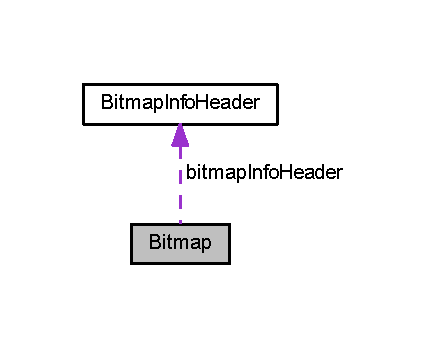
\includegraphics[width=206pt]{struct_bitmap__coll__graph}
\end{center}
\end{figure}
\subsection*{Data Fields}
\begin{DoxyCompactItemize}
\item 
\hyperlink{struct_bitmap_info_header}{Bitmap\+Info\+Header} \hyperlink{struct_bitmap_a7157ca7f3ce4be47481c472fafd89313}{bitmap\+Info\+Header}
\item 
unsigned char $\ast$ \hyperlink{struct_bitmap_a586c4bcc42cf22a033e8f60f24f627f0}{bitmap\+Data}
\end{DoxyCompactItemize}


\subsection{Detailed Description}
Represents a \hyperlink{struct_bitmap}{Bitmap} 

\subsection{Field Documentation}
\mbox{\Hypertarget{struct_bitmap_a586c4bcc42cf22a033e8f60f24f627f0}\label{struct_bitmap_a586c4bcc42cf22a033e8f60f24f627f0}} 
\index{Bitmap@{Bitmap}!bitmap\+Data@{bitmap\+Data}}
\index{bitmap\+Data@{bitmap\+Data}!Bitmap@{Bitmap}}
\subsubsection{\texorpdfstring{bitmap\+Data}{bitmapData}}
{\footnotesize\ttfamily unsigned char$\ast$ bitmap\+Data}

\mbox{\Hypertarget{struct_bitmap_a7157ca7f3ce4be47481c472fafd89313}\label{struct_bitmap_a7157ca7f3ce4be47481c472fafd89313}} 
\index{Bitmap@{Bitmap}!bitmap\+Info\+Header@{bitmap\+Info\+Header}}
\index{bitmap\+Info\+Header@{bitmap\+Info\+Header}!Bitmap@{Bitmap}}
\subsubsection{\texorpdfstring{bitmap\+Info\+Header}{bitmapInfoHeader}}
{\footnotesize\ttfamily \hyperlink{struct_bitmap_info_header}{Bitmap\+Info\+Header} bitmap\+Info\+Header}



The documentation for this struct was generated from the following file\+:\begin{DoxyCompactItemize}
\item 
C\+:/\+Users/\+Nelson/\+Desktop/\+L\+C\+O\+M -\/ 2ºano -\/ 2º semestre/source/\hyperlink{bitmap_8h}{bitmap.\+h}\end{DoxyCompactItemize}

\hypertarget{struct_bitmap_file_header}{}\section{Bitmap\+File\+Header Struct Reference}
\label{struct_bitmap_file_header}\index{Bitmap\+File\+Header@{Bitmap\+File\+Header}}


{\ttfamily \#include $<$bitmap.\+h$>$}

\subsection*{Data Fields}
\begin{DoxyCompactItemize}
\item 
unsigned short \hyperlink{struct_bitmap_file_header_aa929142c5ddf34cf0915c97a617a1a63}{type}
\item 
unsigned int \hyperlink{struct_bitmap_file_header_aac913b3a1f6ef005d66bf7a84428773e}{size}
\item 
unsigned int \hyperlink{struct_bitmap_file_header_a05d5cbcb44f437341bd9fa37d589aced}{reserved}
\item 
unsigned int \hyperlink{struct_bitmap_file_header_a29b5297d3393519050e3126c4cb07c1c}{offset}
\end{DoxyCompactItemize}


\subsection{Detailed Description}
Represents a \hyperlink{struct_bitmap}{Bitmap} File 

\subsection{Field Documentation}
\mbox{\Hypertarget{struct_bitmap_file_header_a29b5297d3393519050e3126c4cb07c1c}\label{struct_bitmap_file_header_a29b5297d3393519050e3126c4cb07c1c}} 
\index{Bitmap\+File\+Header@{Bitmap\+File\+Header}!offset@{offset}}
\index{offset@{offset}!Bitmap\+File\+Header@{Bitmap\+File\+Header}}
\subsubsection{\texorpdfstring{offset}{offset}}
{\footnotesize\ttfamily unsigned int offset}

specifies the offset in bytes from the bitmapfileheader to the bitmap bits \mbox{\Hypertarget{struct_bitmap_file_header_a05d5cbcb44f437341bd9fa37d589aced}\label{struct_bitmap_file_header_a05d5cbcb44f437341bd9fa37d589aced}} 
\index{Bitmap\+File\+Header@{Bitmap\+File\+Header}!reserved@{reserved}}
\index{reserved@{reserved}!Bitmap\+File\+Header@{Bitmap\+File\+Header}}
\subsubsection{\texorpdfstring{reserved}{reserved}}
{\footnotesize\ttfamily unsigned int reserved}

reserved; must be 0 \mbox{\Hypertarget{struct_bitmap_file_header_aac913b3a1f6ef005d66bf7a84428773e}\label{struct_bitmap_file_header_aac913b3a1f6ef005d66bf7a84428773e}} 
\index{Bitmap\+File\+Header@{Bitmap\+File\+Header}!size@{size}}
\index{size@{size}!Bitmap\+File\+Header@{Bitmap\+File\+Header}}
\subsubsection{\texorpdfstring{size}{size}}
{\footnotesize\ttfamily unsigned int size}

specifies the size in bytes of the bitmap file \mbox{\Hypertarget{struct_bitmap_file_header_aa929142c5ddf34cf0915c97a617a1a63}\label{struct_bitmap_file_header_aa929142c5ddf34cf0915c97a617a1a63}} 
\index{Bitmap\+File\+Header@{Bitmap\+File\+Header}!type@{type}}
\index{type@{type}!Bitmap\+File\+Header@{Bitmap\+File\+Header}}
\subsubsection{\texorpdfstring{type}{type}}
{\footnotesize\ttfamily unsigned short type}

specifies the file type 

The documentation for this struct was generated from the following file\+:\begin{DoxyCompactItemize}
\item 
C\+:/\+Users/\+Nelson/\+Desktop/\+L\+C\+O\+M -\/ 2ºano -\/ 2º semestre/source/\hyperlink{bitmap_8h}{bitmap.\+h}\end{DoxyCompactItemize}

\hypertarget{struct_bitmap_info_header}{}\section{Bitmap\+Info\+Header Struct Reference}
\label{struct_bitmap_info_header}\index{Bitmap\+Info\+Header@{Bitmap\+Info\+Header}}


{\ttfamily \#include $<$bitmap.\+h$>$}

\subsection*{Data Fields}
\begin{DoxyCompactItemize}
\item 
unsigned int \hyperlink{struct_bitmap_info_header_aac913b3a1f6ef005d66bf7a84428773e}{size}
\item 
int \hyperlink{struct_bitmap_info_header_a2474a5474cbff19523a51eb1de01cda4}{width}
\item 
int \hyperlink{struct_bitmap_info_header_ad12fc34ce789bce6c8a05d8a17138534}{height}
\item 
unsigned short \hyperlink{struct_bitmap_info_header_a8c89d091e05544a82dc2398eed99634f}{planes}
\item 
unsigned short \hyperlink{struct_bitmap_info_header_a47d1d4d776f8fd3bb0f7dbc3c5aeb534}{bits}
\item 
unsigned int \hyperlink{struct_bitmap_info_header_ad180079f62b44e49ec672c9ef6e078b3}{compression}
\item 
unsigned int \hyperlink{struct_bitmap_info_header_adcd57a0168319e747bc8099218d3822c}{image\+Size}
\item 
int \hyperlink{struct_bitmap_info_header_ac6eaeb4c0876cf6cd899f41fe3c25ff5}{x\+Resolution}
\item 
int \hyperlink{struct_bitmap_info_header_aa2f350dd0bda750656d5db5f5e37b2b3}{y\+Resolution}
\item 
unsigned int \hyperlink{struct_bitmap_info_header_aed4506bad904845183194f199f1bdb98}{n\+Colors}
\item 
unsigned int \hyperlink{struct_bitmap_info_header_a8f7abfbc446b12f385d2b42c3b4fd9b0}{important\+Colors}
\end{DoxyCompactItemize}


\subsection{Detailed Description}
Represents the \hyperlink{struct_bitmap}{Bitmap} information 

\subsection{Field Documentation}
\mbox{\Hypertarget{struct_bitmap_info_header_a47d1d4d776f8fd3bb0f7dbc3c5aeb534}\label{struct_bitmap_info_header_a47d1d4d776f8fd3bb0f7dbc3c5aeb534}} 
\index{Bitmap\+Info\+Header@{Bitmap\+Info\+Header}!bits@{bits}}
\index{bits@{bits}!Bitmap\+Info\+Header@{Bitmap\+Info\+Header}}
\subsubsection{\texorpdfstring{bits}{bits}}
{\footnotesize\ttfamily unsigned short bits}

specifies the number of bit per pixel \mbox{\Hypertarget{struct_bitmap_info_header_ad180079f62b44e49ec672c9ef6e078b3}\label{struct_bitmap_info_header_ad180079f62b44e49ec672c9ef6e078b3}} 
\index{Bitmap\+Info\+Header@{Bitmap\+Info\+Header}!compression@{compression}}
\index{compression@{compression}!Bitmap\+Info\+Header@{Bitmap\+Info\+Header}}
\subsubsection{\texorpdfstring{compression}{compression}}
{\footnotesize\ttfamily unsigned int compression}

specifies the type of compression \mbox{\Hypertarget{struct_bitmap_info_header_ad12fc34ce789bce6c8a05d8a17138534}\label{struct_bitmap_info_header_ad12fc34ce789bce6c8a05d8a17138534}} 
\index{Bitmap\+Info\+Header@{Bitmap\+Info\+Header}!height@{height}}
\index{height@{height}!Bitmap\+Info\+Header@{Bitmap\+Info\+Header}}
\subsubsection{\texorpdfstring{height}{height}}
{\footnotesize\ttfamily int height}

specifies height in pixels \mbox{\Hypertarget{struct_bitmap_info_header_adcd57a0168319e747bc8099218d3822c}\label{struct_bitmap_info_header_adcd57a0168319e747bc8099218d3822c}} 
\index{Bitmap\+Info\+Header@{Bitmap\+Info\+Header}!image\+Size@{image\+Size}}
\index{image\+Size@{image\+Size}!Bitmap\+Info\+Header@{Bitmap\+Info\+Header}}
\subsubsection{\texorpdfstring{image\+Size}{imageSize}}
{\footnotesize\ttfamily unsigned int image\+Size}

size of image in bytes \mbox{\Hypertarget{struct_bitmap_info_header_a8f7abfbc446b12f385d2b42c3b4fd9b0}\label{struct_bitmap_info_header_a8f7abfbc446b12f385d2b42c3b4fd9b0}} 
\index{Bitmap\+Info\+Header@{Bitmap\+Info\+Header}!important\+Colors@{important\+Colors}}
\index{important\+Colors@{important\+Colors}!Bitmap\+Info\+Header@{Bitmap\+Info\+Header}}
\subsubsection{\texorpdfstring{important\+Colors}{importantColors}}
{\footnotesize\ttfamily unsigned int important\+Colors}

number of colors that are important \mbox{\Hypertarget{struct_bitmap_info_header_aed4506bad904845183194f199f1bdb98}\label{struct_bitmap_info_header_aed4506bad904845183194f199f1bdb98}} 
\index{Bitmap\+Info\+Header@{Bitmap\+Info\+Header}!n\+Colors@{n\+Colors}}
\index{n\+Colors@{n\+Colors}!Bitmap\+Info\+Header@{Bitmap\+Info\+Header}}
\subsubsection{\texorpdfstring{n\+Colors}{nColors}}
{\footnotesize\ttfamily unsigned int n\+Colors}

number of colors used by the bitmap \mbox{\Hypertarget{struct_bitmap_info_header_a8c89d091e05544a82dc2398eed99634f}\label{struct_bitmap_info_header_a8c89d091e05544a82dc2398eed99634f}} 
\index{Bitmap\+Info\+Header@{Bitmap\+Info\+Header}!planes@{planes}}
\index{planes@{planes}!Bitmap\+Info\+Header@{Bitmap\+Info\+Header}}
\subsubsection{\texorpdfstring{planes}{planes}}
{\footnotesize\ttfamily unsigned short planes}

specifies the number of color planes, must be 1 \mbox{\Hypertarget{struct_bitmap_info_header_aac913b3a1f6ef005d66bf7a84428773e}\label{struct_bitmap_info_header_aac913b3a1f6ef005d66bf7a84428773e}} 
\index{Bitmap\+Info\+Header@{Bitmap\+Info\+Header}!size@{size}}
\index{size@{size}!Bitmap\+Info\+Header@{Bitmap\+Info\+Header}}
\subsubsection{\texorpdfstring{size}{size}}
{\footnotesize\ttfamily unsigned int size}

specifies the number of bytes required by the struct \mbox{\Hypertarget{struct_bitmap_info_header_a2474a5474cbff19523a51eb1de01cda4}\label{struct_bitmap_info_header_a2474a5474cbff19523a51eb1de01cda4}} 
\index{Bitmap\+Info\+Header@{Bitmap\+Info\+Header}!width@{width}}
\index{width@{width}!Bitmap\+Info\+Header@{Bitmap\+Info\+Header}}
\subsubsection{\texorpdfstring{width}{width}}
{\footnotesize\ttfamily int width}

specifies width in pixels \mbox{\Hypertarget{struct_bitmap_info_header_ac6eaeb4c0876cf6cd899f41fe3c25ff5}\label{struct_bitmap_info_header_ac6eaeb4c0876cf6cd899f41fe3c25ff5}} 
\index{Bitmap\+Info\+Header@{Bitmap\+Info\+Header}!x\+Resolution@{x\+Resolution}}
\index{x\+Resolution@{x\+Resolution}!Bitmap\+Info\+Header@{Bitmap\+Info\+Header}}
\subsubsection{\texorpdfstring{x\+Resolution}{xResolution}}
{\footnotesize\ttfamily int x\+Resolution}

number of pixels per meter in x axis \mbox{\Hypertarget{struct_bitmap_info_header_aa2f350dd0bda750656d5db5f5e37b2b3}\label{struct_bitmap_info_header_aa2f350dd0bda750656d5db5f5e37b2b3}} 
\index{Bitmap\+Info\+Header@{Bitmap\+Info\+Header}!y\+Resolution@{y\+Resolution}}
\index{y\+Resolution@{y\+Resolution}!Bitmap\+Info\+Header@{Bitmap\+Info\+Header}}
\subsubsection{\texorpdfstring{y\+Resolution}{yResolution}}
{\footnotesize\ttfamily int y\+Resolution}

number of pixels per meter in y axis 

The documentation for this struct was generated from the following file\+:\begin{DoxyCompactItemize}
\item 
C\+:/\+Users/\+Nelson/\+Desktop/\+L\+C\+O\+M -\/ 2ºano -\/ 2º semestre/source/\hyperlink{bitmap_8h}{bitmap.\+h}\end{DoxyCompactItemize}

\chapter{File Documentation}
\hypertarget{bitmap_8c}{}\section{C\+:/\+Users/\+Nelson/\+Desktop/\+L\+C\+OM -\/ 2ºano -\/ 2º semestre/source/bitmap.c File Reference}
\label{bitmap_8c}\index{C\+:/\+Users/\+Nelson/\+Desktop/\+L\+C\+O\+M -\/ 2ºano -\/ 2º semestre/source/bitmap.\+c@{C\+:/\+Users/\+Nelson/\+Desktop/\+L\+C\+O\+M -\/ 2ºano -\/ 2º semestre/source/bitmap.\+c}}
{\ttfamily \#include \char`\"{}bitmap.\+h\char`\"{}}\newline
{\ttfamily \#include $<$minix/syslib.\+h$>$}\newline
{\ttfamily \#include $<$minix/drivers.\+h$>$}\newline
{\ttfamily \#include $<$machine/int86.\+h$>$}\newline
{\ttfamily \#include \char`\"{}stdio.\+h\char`\"{}}\newline
{\ttfamily \#include \char`\"{}video\+\_\+gr.\+h\char`\"{}}\newline
{\ttfamily \#include \char`\"{}timer.\+h\char`\"{}}\newline
{\ttfamily \#include \char`\"{}gamevariables.\+h\char`\"{}}\newline
Include dependency graph for bitmap.\+c\+:
\nopagebreak
\begin{figure}[H]
\begin{center}
\leavevmode
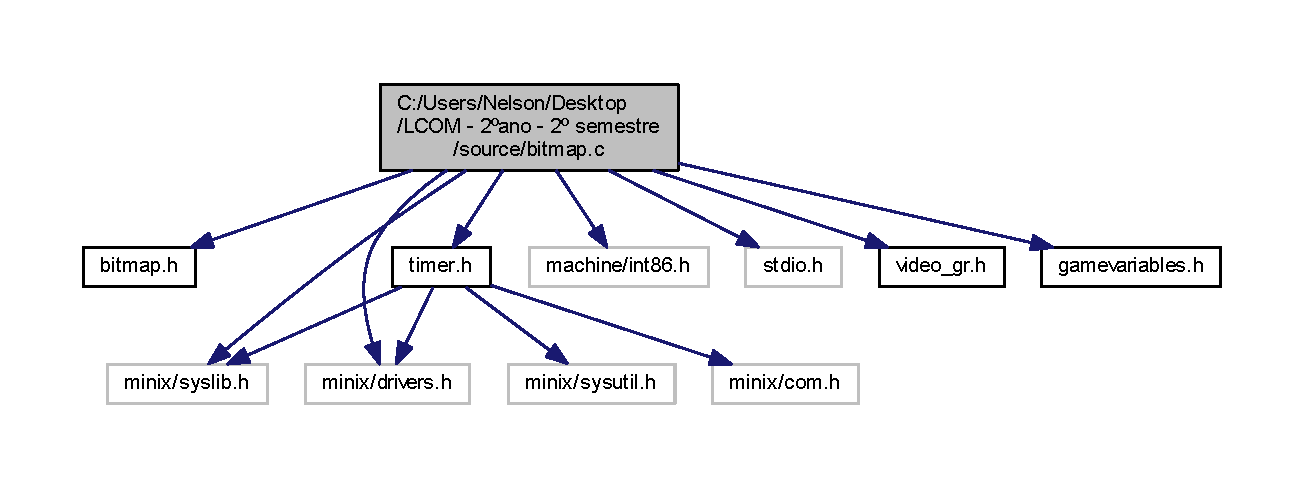
\includegraphics[width=350pt]{bitmap_8c__incl}
\end{center}
\end{figure}
\subsection*{Functions}
\begin{DoxyCompactItemize}
\item 
\hyperlink{struct_bitmap}{Bitmap} $\ast$ \hyperlink{group___bitmap_ga3506880ffd407c36eb8aaddd2c1606d2}{load\+Bitmap} (const char $\ast$filename)
\begin{DoxyCompactList}\small\item\em Loads a bmp image. \end{DoxyCompactList}\item 
void \hyperlink{group___bitmap_ga18d05a1c671f4638bc63d37874efb9d4}{draw\+Bitmap} (\hyperlink{struct_bitmap}{Bitmap} $\ast$bmp, int x, int y, \hyperlink{group___bitmap_gacdfaca60ec19c0265bac2692d7982726}{Alignment} alignment)
\begin{DoxyCompactList}\small\item\em Draws an unscaled, unrotated bitmap at the given position. \end{DoxyCompactList}\item 
void \hyperlink{group___bitmap_ga08c1d4f4fff81df260d979ea8fc1aa61}{delete\+Bitmap} (\hyperlink{struct_bitmap}{Bitmap} $\ast$bmp)
\begin{DoxyCompactList}\small\item\em Destroys the given bitmap, freeing all resources used by it. \end{DoxyCompactList}\item 
void \hyperlink{group___bitmap_gabda6654c65348aa9c06a9ae0e9562b9a}{get\+\_\+bitmaps} ()
\begin{DoxyCompactList}\small\item\em Loads all the bitmaps used by calling load\+Bitmap function. \end{DoxyCompactList}\item 
void \hyperlink{group___bitmap_ga66c6cdf9473527bd3dcbab53d147d5b9}{draw\+\_\+black\+\_\+screen} ()
\begin{DoxyCompactList}\small\item\em Draws a black screen using the black bar image. \end{DoxyCompactList}\item 
void \hyperlink{group___bitmap_ga83361e027b6f0dd917305f1f82dedda3}{draw\+\_\+main\+\_\+menu} ()
\begin{DoxyCompactList}\small\item\em Draws the main menu, wich gives you two options\+: S\+T\+A\+RT or E\+X\+IT. \end{DoxyCompactList}\item 
void \hyperlink{group___bitmap_gaa7519d8a181750afa183c3350c5f9598}{draw\+\_\+board} (int \hyperlink{game_8c_a0b7685156d686874cf7a3f95a6b7f3f3}{round})
\begin{DoxyCompactList}\small\item\em Draws the game board, environment in wich the game will decurr (the gaming board shows the current round). \end{DoxyCompactList}\item 
void \hyperlink{group___bitmap_gaca0d178c01fee283d1e3386b9712736e}{draw\+\_\+player1\+\_\+turn} ()
\begin{DoxyCompactList}\small\item\em A draw that announces player1\textquotesingle{}s turn to play. \end{DoxyCompactList}\item 
void \hyperlink{group___bitmap_ga9af400ed66deb4c3aff712d9a7e9f522}{draw\+\_\+player2\+\_\+turn} ()
\begin{DoxyCompactList}\small\item\em A draw that announces player2\textquotesingle{}s turn to play. \end{DoxyCompactList}\item 
void \hyperlink{bitmap_8c_a9c8f7086bfab6b8558ab5fdfca5e4e63}{draw\+\_\+successful\+\_\+copy} ()
\item 
void \hyperlink{group___bitmap_ga06ba1c351da1ccdfa323137861c1a9af}{draw\+\_\+failed\+\_\+copy} ()
\begin{DoxyCompactList}\small\item\em A draw that announces a failed copy of player1\textquotesingle{}s moves. \end{DoxyCompactList}\item 
void \hyperlink{group___bitmap_gabbf5153c909fc82e7734744352e22de9}{draw\+\_\+thanks\+\_\+for\+\_\+playing} ()
\begin{DoxyCompactList}\small\item\em A draw that says \char`\"{}\+Thank you for playing\char`\"{}. \end{DoxyCompactList}\item 
void \hyperlink{group___bitmap_ga556f9cfc8664aff3169e9775310a5144}{draw\+\_\+input} (int input)
\begin{DoxyCompactList}\small\item\em A draws a given input given by a player. an input is a play made by a player (it can be selecting a geometrical figure on the board, preesing a key, or draw a positive slope with the mouse) \end{DoxyCompactList}\item 
void \hyperlink{group___bitmap_ga108608b0f2d804c84a271547036b6ffd}{draw\+\_\+cursor} (int x, int y)
\begin{DoxyCompactList}\small\item\em Draws the mouse cursor at a given location. \end{DoxyCompactList}\item 
void \hyperlink{bitmap_8c_afd011e7c56424f96bba293494afa1f2c}{draw\+\_\+score} (int score)
\item 
void \hyperlink{group___bitmap_ga97df0f6e4184d84c9e3871042b94bc3a}{draw\+\_\+number} (int number, int x, int y)
\begin{DoxyCompactList}\small\item\em Draws a number(0-\/9) at a given location(x,y) \end{DoxyCompactList}\end{DoxyCompactItemize}


\subsection{Function Documentation}
\mbox{\Hypertarget{bitmap_8c_afd011e7c56424f96bba293494afa1f2c}\label{bitmap_8c_afd011e7c56424f96bba293494afa1f2c}} 
\index{bitmap.\+c@{bitmap.\+c}!draw\+\_\+score@{draw\+\_\+score}}
\index{draw\+\_\+score@{draw\+\_\+score}!bitmap.\+c@{bitmap.\+c}}
\subsubsection{\texorpdfstring{draw\+\_\+score()}{draw\_score()}}
{\footnotesize\ttfamily void draw\+\_\+score (\begin{DoxyParamCaption}\item[{int}]{score }\end{DoxyParamCaption})}

Here is the call graph for this function\+:\nopagebreak
\begin{figure}[H]
\begin{center}
\leavevmode
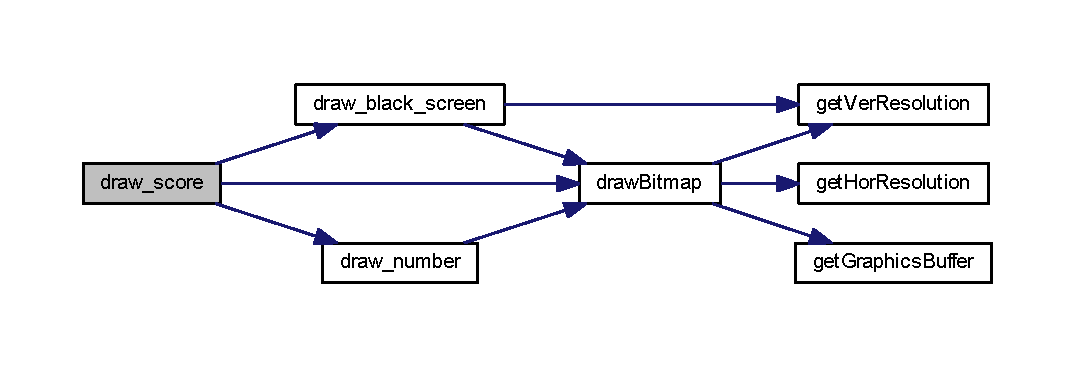
\includegraphics[width=350pt]{bitmap_8c_afd011e7c56424f96bba293494afa1f2c_cgraph}
\end{center}
\end{figure}
Here is the caller graph for this function\+:\nopagebreak
\begin{figure}[H]
\begin{center}
\leavevmode
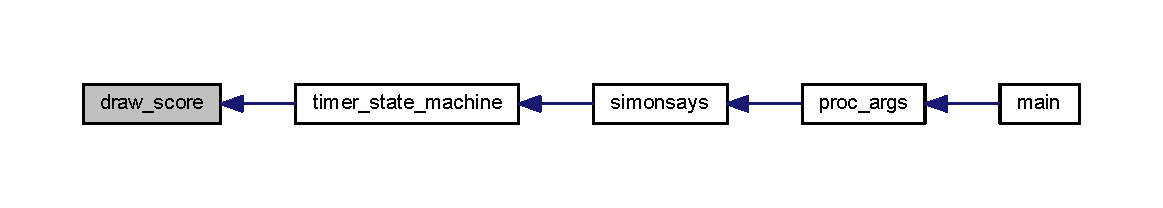
\includegraphics[width=350pt]{bitmap_8c_afd011e7c56424f96bba293494afa1f2c_icgraph}
\end{center}
\end{figure}
\mbox{\Hypertarget{bitmap_8c_a9c8f7086bfab6b8558ab5fdfca5e4e63}\label{bitmap_8c_a9c8f7086bfab6b8558ab5fdfca5e4e63}} 
\index{bitmap.\+c@{bitmap.\+c}!draw\+\_\+successful\+\_\+copy@{draw\+\_\+successful\+\_\+copy}}
\index{draw\+\_\+successful\+\_\+copy@{draw\+\_\+successful\+\_\+copy}!bitmap.\+c@{bitmap.\+c}}
\subsubsection{\texorpdfstring{draw\+\_\+successful\+\_\+copy()}{draw\_successful\_copy()}}
{\footnotesize\ttfamily void draw\+\_\+successful\+\_\+copy (\begin{DoxyParamCaption}{ }\end{DoxyParamCaption})}

Here is the call graph for this function\+:\nopagebreak
\begin{figure}[H]
\begin{center}
\leavevmode
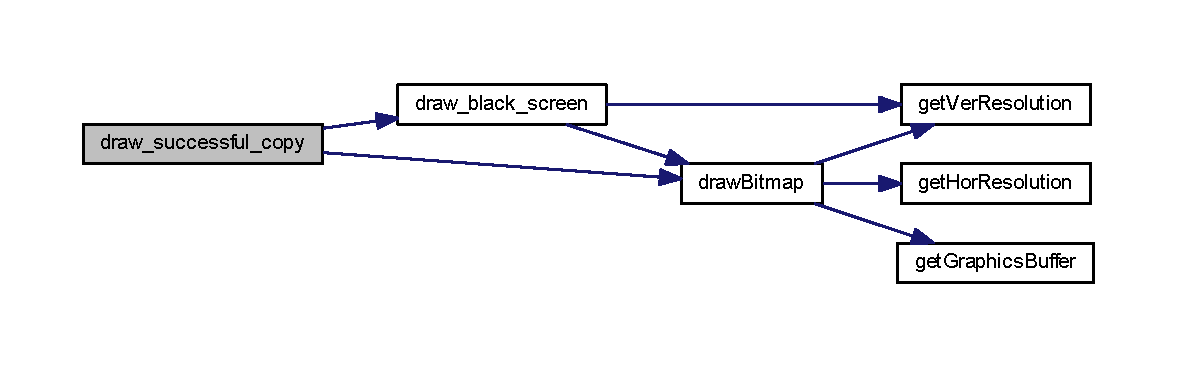
\includegraphics[width=350pt]{bitmap_8c_a9c8f7086bfab6b8558ab5fdfca5e4e63_cgraph}
\end{center}
\end{figure}
Here is the caller graph for this function\+:\nopagebreak
\begin{figure}[H]
\begin{center}
\leavevmode
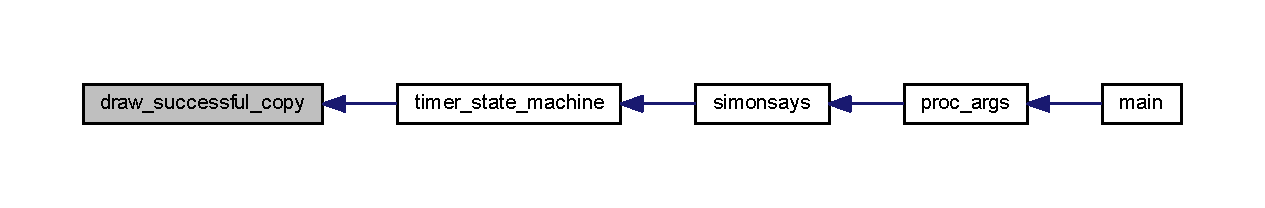
\includegraphics[width=350pt]{bitmap_8c_a9c8f7086bfab6b8558ab5fdfca5e4e63_icgraph}
\end{center}
\end{figure}

\hypertarget{bitmap_8h}{}\section{C\+:/\+Users/\+Nelson/\+Desktop/\+L\+C\+OM -\/ 2ºano -\/ 2º semestre/source/bitmap.h File Reference}
\label{bitmap_8h}\index{C\+:/\+Users/\+Nelson/\+Desktop/\+L\+C\+O\+M -\/ 2ºano -\/ 2º semestre/source/bitmap.\+h@{C\+:/\+Users/\+Nelson/\+Desktop/\+L\+C\+O\+M -\/ 2ºano -\/ 2º semestre/source/bitmap.\+h}}
This graph shows which files directly or indirectly include this file\+:
\nopagebreak
\begin{figure}[H]
\begin{center}
\leavevmode
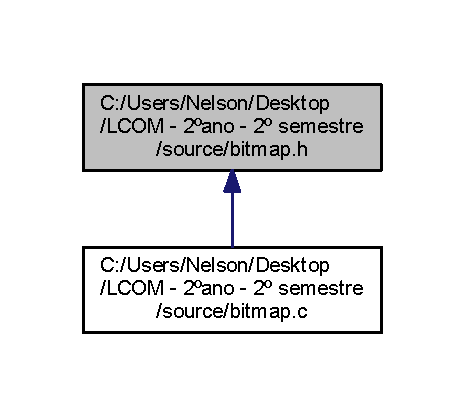
\includegraphics[width=223pt]{bitmap_8h__dep__incl}
\end{center}
\end{figure}
\subsection*{Data Structures}
\begin{DoxyCompactItemize}
\item 
struct \hyperlink{struct_bitmap_file_header}{Bitmap\+File\+Header}
\item 
struct \hyperlink{struct_bitmap_info_header}{Bitmap\+Info\+Header}
\item 
struct \hyperlink{struct_bitmap}{Bitmap}
\end{DoxyCompactItemize}
\subsection*{Enumerations}
\begin{DoxyCompactItemize}
\item 
enum \hyperlink{group___bitmap_gacdfaca60ec19c0265bac2692d7982726}{Alignment} \{ \hyperlink{group___bitmap_ggacdfaca60ec19c0265bac2692d7982726a6ec599857e15466988726932dd592305}{A\+L\+I\+G\+N\+\_\+\+L\+E\+FT}, 
\hyperlink{group___bitmap_ggacdfaca60ec19c0265bac2692d7982726a5624165187e56db612253e608a45b1c6}{A\+L\+I\+G\+N\+\_\+\+C\+E\+N\+T\+ER}, 
\hyperlink{group___bitmap_ggacdfaca60ec19c0265bac2692d7982726a9c81840e8cad46418b39a8b74a246354}{A\+L\+I\+G\+N\+\_\+\+R\+I\+G\+HT}
 \}
\end{DoxyCompactItemize}
\subsection*{Functions}
\begin{DoxyCompactItemize}
\item 
\hyperlink{struct_bitmap}{Bitmap} $\ast$ \hyperlink{group___bitmap_ga3506880ffd407c36eb8aaddd2c1606d2}{load\+Bitmap} (const char $\ast$filename)
\begin{DoxyCompactList}\small\item\em Loads a bmp image. \end{DoxyCompactList}\item 
void \hyperlink{group___bitmap_ga18d05a1c671f4638bc63d37874efb9d4}{draw\+Bitmap} (\hyperlink{struct_bitmap}{Bitmap} $\ast$bitmap, int x, int y, \hyperlink{group___bitmap_gacdfaca60ec19c0265bac2692d7982726}{Alignment} alignment)
\begin{DoxyCompactList}\small\item\em Draws an unscaled, unrotated bitmap at the given position. \end{DoxyCompactList}\item 
void \hyperlink{group___bitmap_ga08c1d4f4fff81df260d979ea8fc1aa61}{delete\+Bitmap} (\hyperlink{struct_bitmap}{Bitmap} $\ast$bmp)
\begin{DoxyCompactList}\small\item\em Destroys the given bitmap, freeing all resources used by it. \end{DoxyCompactList}\item 
void \hyperlink{group___bitmap_gabda6654c65348aa9c06a9ae0e9562b9a}{get\+\_\+bitmaps} ()
\begin{DoxyCompactList}\small\item\em Loads all the bitmaps used by calling load\+Bitmap function. \end{DoxyCompactList}\item 
void \hyperlink{group___bitmap_ga66c6cdf9473527bd3dcbab53d147d5b9}{draw\+\_\+black\+\_\+screen} ()
\begin{DoxyCompactList}\small\item\em Draws a black screen using the black bar image. \end{DoxyCompactList}\item 
void \hyperlink{group___bitmap_ga83361e027b6f0dd917305f1f82dedda3}{draw\+\_\+main\+\_\+menu} ()
\begin{DoxyCompactList}\small\item\em Draws the main menu, wich gives you two options\+: S\+T\+A\+RT or E\+X\+IT. \end{DoxyCompactList}\item 
void \hyperlink{group___bitmap_gaa7519d8a181750afa183c3350c5f9598}{draw\+\_\+board} (int \hyperlink{game_8c_a0b7685156d686874cf7a3f95a6b7f3f3}{round})
\begin{DoxyCompactList}\small\item\em Draws the game board, environment in wich the game will decurr (the gaming board shows the current round). \end{DoxyCompactList}\item 
void \hyperlink{group___bitmap_gaca0d178c01fee283d1e3386b9712736e}{draw\+\_\+player1\+\_\+turn} ()
\begin{DoxyCompactList}\small\item\em A draw that announces player1\textquotesingle{}s turn to play. \end{DoxyCompactList}\item 
void \hyperlink{group___bitmap_ga9af400ed66deb4c3aff712d9a7e9f522}{draw\+\_\+player2\+\_\+turn} ()
\begin{DoxyCompactList}\small\item\em A draw that announces player2\textquotesingle{}s turn to play. \end{DoxyCompactList}\item 
void \hyperlink{group___bitmap_gae696a3d4ee82a15e937f5f8c11fa9057}{draw\+\_\+success\+\_\+copy} ()
\begin{DoxyCompactList}\small\item\em A draw that announces a successful copy of player1\textquotesingle{}s moves. \end{DoxyCompactList}\item 
void \hyperlink{group___bitmap_ga06ba1c351da1ccdfa323137861c1a9af}{draw\+\_\+failed\+\_\+copy} ()
\begin{DoxyCompactList}\small\item\em A draw that announces a failed copy of player1\textquotesingle{}s moves. \end{DoxyCompactList}\item 
void \hyperlink{group___bitmap_gabbf5153c909fc82e7734744352e22de9}{draw\+\_\+thanks\+\_\+for\+\_\+playing} ()
\begin{DoxyCompactList}\small\item\em A draw that says \char`\"{}\+Thank you for playing\char`\"{}. \end{DoxyCompactList}\item 
void \hyperlink{group___bitmap_ga556f9cfc8664aff3169e9775310a5144}{draw\+\_\+input} (int input)
\begin{DoxyCompactList}\small\item\em A draws a given input given by a player. an input is a play made by a player (it can be selecting a geometrical figure on the board, preesing a key, or draw a positive slope with the mouse) \end{DoxyCompactList}\item 
void \hyperlink{group___bitmap_ga108608b0f2d804c84a271547036b6ffd}{draw\+\_\+cursor} (int x, int y)
\begin{DoxyCompactList}\small\item\em Draws the mouse cursor at a given location. \end{DoxyCompactList}\item 
void \hyperlink{group___bitmap_ga97df0f6e4184d84c9e3871042b94bc3a}{draw\+\_\+number} (int number, int x, int y)
\begin{DoxyCompactList}\small\item\em Draws a number(0-\/9) at a given location(x,y) \end{DoxyCompactList}\end{DoxyCompactItemize}
\subsection*{Variables}
\begin{DoxyCompactItemize}
\item 
\hyperlink{struct_bitmap}{Bitmap} $\ast$ \hyperlink{group___bitmap_gaf1aaa82e6e29c903bb1fda96ce708d27}{bitmap\+\_\+welcome}
\item 
\hyperlink{struct_bitmap}{Bitmap} $\ast$ \hyperlink{group___bitmap_ga5240b87601f0b5aa3e67976c3ed240ed}{bitmap\+\_\+to}
\item 
\hyperlink{struct_bitmap}{Bitmap} $\ast$ \hyperlink{group___bitmap_ga7cad4ac90d452221efb12d6156b53b22}{bitmap\+\_\+simonsays}
\item 
\hyperlink{struct_bitmap}{Bitmap} $\ast$ \hyperlink{group___bitmap_ga87c8ef496268863adc00746941f79f44}{bitmap\+\_\+start}
\item 
\hyperlink{struct_bitmap}{Bitmap} $\ast$ \hyperlink{group___bitmap_ga952f653fe87f4ca995595e2b7db6228f}{bitmap\+\_\+exit}
\item 
\hyperlink{struct_bitmap}{Bitmap} $\ast$ \hyperlink{group___bitmap_gaf81c286e8b6c034dd42b1e09dfb4c9d9}{bitmap\+\_\+triangle}
\item 
\hyperlink{struct_bitmap}{Bitmap} $\ast$ \hyperlink{group___bitmap_gac1d843b74dd56e98adf0c72f75a5a1d8}{bitmap\+\_\+circle}
\item 
\hyperlink{struct_bitmap}{Bitmap} $\ast$ \hyperlink{group___bitmap_gacf0c500ba60d2cf03c116fe731b21ec9}{bitmap\+\_\+star}
\item 
\hyperlink{struct_bitmap}{Bitmap} $\ast$ \hyperlink{group___bitmap_gaa6ea6c52c8712671d8ed350cde2f2313}{bitmap\+\_\+square}
\item 
\hyperlink{struct_bitmap}{Bitmap} $\ast$ \hyperlink{group___bitmap_ga19d13e384604a13b7d8a0839aadd9234}{bitmap\+\_\+vertical\+\_\+white\+\_\+bar}
\item 
\hyperlink{struct_bitmap}{Bitmap} $\ast$ \hyperlink{group___bitmap_ga4610248f579630fea652a3704556c74c}{bitmap\+\_\+horizontal\+\_\+white\+\_\+bar}
\item 
\hyperlink{struct_bitmap}{Bitmap} $\ast$ \hyperlink{group___bitmap_gac6d8af40b0549ee19c8d2d146ac2844f}{bitmap\+\_\+last\+\_\+input}
\item 
\hyperlink{struct_bitmap}{Bitmap} $\ast$ \hyperlink{group___bitmap_ga2f913b78a0f833c9a04aef7f4b334062}{bitmap\+\_\+round}
\item 
\hyperlink{struct_bitmap}{Bitmap} $\ast$ \hyperlink{group___bitmap_ga993712c0e2465ddf6682e1da844cb33f}{bitmap\+\_\+number\+\_\+0}
\item 
\hyperlink{struct_bitmap}{Bitmap} $\ast$ \hyperlink{group___bitmap_gae0e099ab280db078712dae7370590d69}{bitmap\+\_\+number\+\_\+1}
\item 
\hyperlink{struct_bitmap}{Bitmap} $\ast$ \hyperlink{group___bitmap_gabff0396d599ff9c20dc45260ac0023e3}{bitmap\+\_\+number\+\_\+2}
\item 
\hyperlink{struct_bitmap}{Bitmap} $\ast$ \hyperlink{group___bitmap_ga691847399b96e5814e96eaa88d89a565}{bitmap\+\_\+number\+\_\+3}
\item 
\hyperlink{struct_bitmap}{Bitmap} $\ast$ \hyperlink{group___bitmap_ga0d04224487333eb3e7b5e2f6f84c0c7c}{bitmap\+\_\+number\+\_\+4}
\item 
\hyperlink{struct_bitmap}{Bitmap} $\ast$ \hyperlink{group___bitmap_ga2462605cb4d4dee9006653ffafe12fbc}{bitmap\+\_\+number\+\_\+5}
\item 
\hyperlink{struct_bitmap}{Bitmap} $\ast$ \hyperlink{group___bitmap_ga70b99f25995d8138d51132de297e66ba}{bitmap\+\_\+number\+\_\+6}
\item 
\hyperlink{struct_bitmap}{Bitmap} $\ast$ \hyperlink{group___bitmap_ga8c4df34a71fbac148bc9ace8ba6095fa}{bitmap\+\_\+number\+\_\+7}
\item 
\hyperlink{struct_bitmap}{Bitmap} $\ast$ \hyperlink{group___bitmap_ga0b28cdc22a12665fb94f55d1c9d269f2}{bitmap\+\_\+number\+\_\+8}
\item 
\hyperlink{struct_bitmap}{Bitmap} $\ast$ \hyperlink{group___bitmap_ga8af434fd1017cdac47579582bac12552}{bitmap\+\_\+number\+\_\+9}
\item 
\hyperlink{struct_bitmap}{Bitmap} $\ast$ \hyperlink{group___bitmap_ga3a3b4fedabcc22d1b0f34e651fcfdb46}{bitmap\+\_\+black\+\_\+square}
\item 
\hyperlink{struct_bitmap}{Bitmap} $\ast$ \hyperlink{group___bitmap_ga508d397d656733b6434a84217519cf27}{bitmap\+\_\+a\+\_\+key}
\item 
\hyperlink{struct_bitmap}{Bitmap} $\ast$ \hyperlink{group___bitmap_ga4f21d75b1561dd84963d37fb8149544b}{bitmap\+\_\+w\+\_\+key}
\item 
\hyperlink{struct_bitmap}{Bitmap} $\ast$ \hyperlink{group___bitmap_gaec5fd5db7147e57f72076387bc78ffc9}{bitmap\+\_\+s\+\_\+key}
\item 
\hyperlink{struct_bitmap}{Bitmap} $\ast$ \hyperlink{group___bitmap_ga3887cbeee8746670c47e70090cc926ae}{bitmap\+\_\+d\+\_\+key}
\item 
\hyperlink{struct_bitmap}{Bitmap} $\ast$ \hyperlink{group___bitmap_ga25ccce5a865640e111d5c3e6fd8405f5}{bitmap\+\_\+black\+\_\+bar}
\item 
\hyperlink{struct_bitmap}{Bitmap} $\ast$ \hyperlink{group___bitmap_ga2ba19da7f92ccbe27fd209c98816837a}{bitmap\+\_\+player1}
\item 
\hyperlink{struct_bitmap}{Bitmap} $\ast$ \hyperlink{group___bitmap_ga63e9b3ca144cce02448900ffe9add6c4}{bitmap\+\_\+player2}
\item 
\hyperlink{struct_bitmap}{Bitmap} $\ast$ \hyperlink{group___bitmap_ga4eb982d201096abdac3cacd3f6459ff2}{bitmap\+\_\+cpu}
\item 
\hyperlink{struct_bitmap}{Bitmap} $\ast$ \hyperlink{group___bitmap_ga6fa1dd9e73670e1d22f5b6d258eb0e77}{bitmap\+\_\+turn}
\item 
\hyperlink{struct_bitmap}{Bitmap} $\ast$ \hyperlink{group___bitmap_gae897f24816ba9a98f564b2b7ff488bc2}{bitmap\+\_\+cursor}
\item 
\hyperlink{struct_bitmap}{Bitmap} $\ast$ \hyperlink{group___bitmap_ga1f04a1ac0e8402f5de2230baf1f6818d}{bitmap\+\_\+congratulations}
\item 
\hyperlink{struct_bitmap}{Bitmap} $\ast$ \hyperlink{group___bitmap_gaf4ba721599394ebe28ce58f495fa1226}{bitmap\+\_\+nice}
\item 
\hyperlink{struct_bitmap}{Bitmap} $\ast$ \hyperlink{group___bitmap_ga68d193359f4b1253056be87ab752f5f0}{bitmap\+\_\+plagiarism}
\item 
\hyperlink{struct_bitmap}{Bitmap} $\ast$ \hyperlink{group___bitmap_ga47000f83189d2a2f74f1148050ee338b}{bitmap\+\_\+happy\+\_\+face}
\item 
\hyperlink{struct_bitmap}{Bitmap} $\ast$ \hyperlink{group___bitmap_gaaedffcc0ad02fe92aaae449a289619e3}{bitmap\+\_\+ups}
\item 
\hyperlink{struct_bitmap}{Bitmap} $\ast$ \hyperlink{group___bitmap_gacc8a2c20312c8ec30b84297cbf6df6f2}{bitmap\+\_\+you}
\item 
\hyperlink{struct_bitmap}{Bitmap} $\ast$ \hyperlink{group___bitmap_ga5d96b14aaf8cbac173f6d809be1ff7d4}{bitmap\+\_\+failed}
\item 
\hyperlink{struct_bitmap}{Bitmap} $\ast$ \hyperlink{group___bitmap_ga712c5447dd57d83342185a9ac9ca7015}{bitmap\+\_\+sad\+\_\+face}
\item 
\hyperlink{struct_bitmap}{Bitmap} $\ast$ \hyperlink{group___bitmap_ga227e788aa82989593af33621bfb230bd}{bitmap\+\_\+thanks}
\item 
\hyperlink{struct_bitmap}{Bitmap} $\ast$ \hyperlink{group___bitmap_ga04b3490379f60798e7a6de171979a90f}{bitmap\+\_\+for}
\item 
\hyperlink{struct_bitmap}{Bitmap} $\ast$ \hyperlink{group___bitmap_ga57060e5b51d9603d9fc393526c965a3b}{bitmap\+\_\+playing}
\item 
\hyperlink{struct_bitmap}{Bitmap} $\ast$ \hyperlink{group___bitmap_gacb59d00d1a96d8b830bddde99bc4f7dd}{bitmap\+\_\+final\+\_\+score}
\end{DoxyCompactItemize}

\hypertarget{game_8c}{}\section{C\+:/\+Users/\+Nelson/\+Desktop/\+L\+C\+OM -\/ 2ºano -\/ 2º semestre/source/game.c File Reference}
\label{game_8c}\index{C\+:/\+Users/\+Nelson/\+Desktop/\+L\+C\+O\+M -\/ 2ºano -\/ 2º semestre/source/game.\+c@{C\+:/\+Users/\+Nelson/\+Desktop/\+L\+C\+O\+M -\/ 2ºano -\/ 2º semestre/source/game.\+c}}
{\ttfamily \#include \char`\"{}game.\+h\char`\"{}}\newline
Include dependency graph for game.\+c\+:
\nopagebreak
\begin{figure}[H]
\begin{center}
\leavevmode
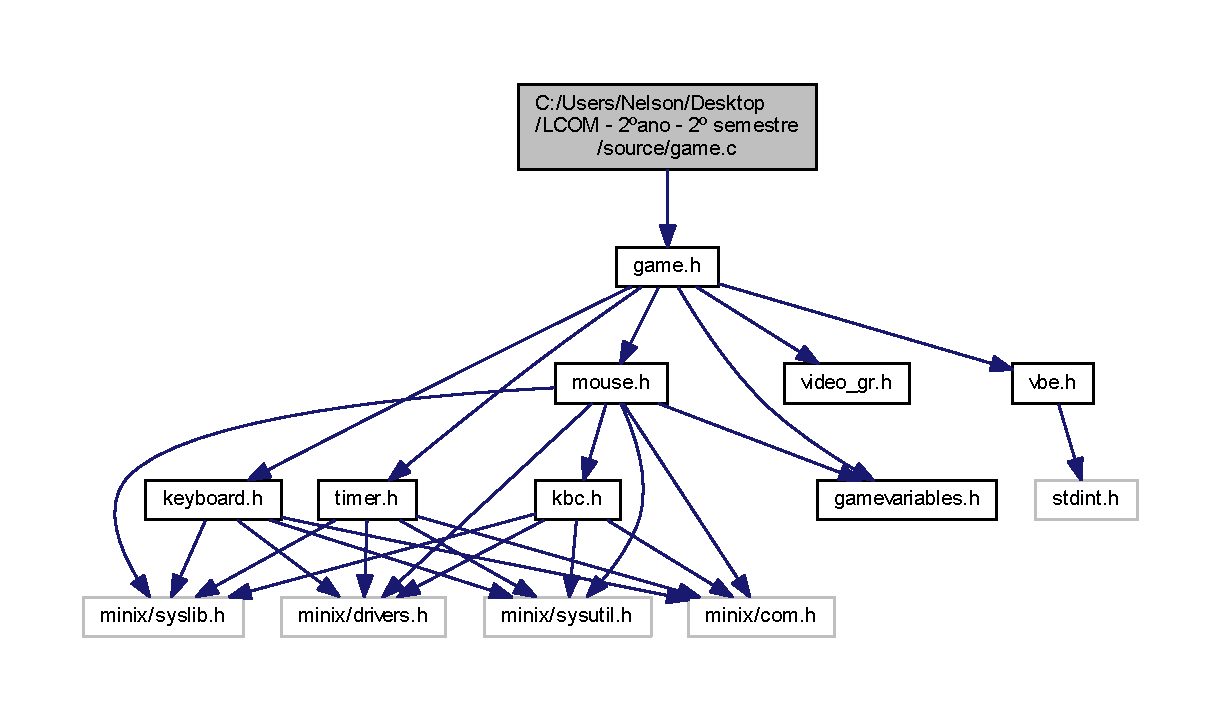
\includegraphics[width=350pt]{game_8c__incl}
\end{center}
\end{figure}
\subsection*{Functions}
\begin{DoxyCompactItemize}
\item 
int \hyperlink{game_8c_a434350c0629d48af15132bd626ff0e7b}{simonsays} ()
\begin{DoxyCompactList}\small\item\em main function that calls the game interruption handlers and the game state machine funtions \end{DoxyCompactList}\item 
void \hyperlink{game_8c_a8101733e49b7935d3b1b8d2bb83dd42f}{state\+\_\+machine} (int input)
\begin{DoxyCompactList}\small\item\em state machine that changes the game state according to the inputs given by the players \end{DoxyCompactList}\item 
int \hyperlink{game_8c_a0ba54f993c5072ccad6ef0562e36443b}{timer\+\_\+state\+\_\+machine} (int input)
\begin{DoxyCompactList}\small\item\em state machine that changes the game state according to the inputs given by the players ,makes the time pauses and draws the screen according to the current state \end{DoxyCompactList}\item 
int \hyperlink{game_8c_a7bd272e601a5455dea734c829bf0feb4}{check\+Timeout} (int pause\+\_\+time)
\begin{DoxyCompactList}\small\item\em is used to make a timeout(wait a number of seconds without doing anything) \end{DoxyCompactList}\item 
int \hyperlink{game_8c_acee4b53c87749506d4f93ed0bdd32ccb}{compare\+\_\+arrays} (int $\ast$array1, int $\ast$array2, int size)
\begin{DoxyCompactList}\small\item\em compares the first size positions of two arrays \end{DoxyCompactList}\end{DoxyCompactItemize}
\subsection*{Variables}
\begin{DoxyCompactItemize}
\item 
static int \hyperlink{game_8c_acf78d5ab53d26add4184578b9732a6a0}{escape} = 0
\item 
static int \hyperlink{game_8c_a312bc2c706f64a3ba78f54cad26d9402}{player2\+\_\+score} =0
\item 
static int \hyperlink{game_8c_a0d7ec96959b5e2328cb30a4a7e7dda10}{player1\+\_\+array} \mbox{[}10\mbox{]}
\item 
static int \hyperlink{game_8c_a08cc02a3fdfc39ca7dce0da405d46872}{player2\+\_\+array} \mbox{[}10\mbox{]}
\item 
static int \hyperlink{game_8c_a401e942526aac47cef94f478182486e7}{position} =0
\item 
static int \hyperlink{game_8c_a493b57f443cc38b3d3df9c1e584d9d82}{timeout} =0
\item 
static int \hyperlink{game_8c_a4c5da45addccd0b2a643a6b73c2f3214}{timeout\+\_\+started} =0
\item 
static int \hyperlink{game_8c_a50f7ef6ef3124abc70fbd30e6c5f06ce}{timeout\+\_\+entered} =0
\item 
static unsigned int \hyperlink{game_8c_ab54283a672f4b80136585c9973814206}{timer\+\_\+counter} =0
\item 
static unsigned int \hyperlink{game_8c_a83e57ce9bd59cfa0995c2e2c8589c274}{time} = 0
\item 
static unsigned int \hyperlink{game_8c_a0b7685156d686874cf7a3f95a6b7f3f3}{round} = 1
\item 
static int \hyperlink{game_8c_ab2623c3ab961285567b984a662aa0a26}{mouse\+\_\+x\+\_\+coord}
\item 
static int \hyperlink{game_8c_aadada65942cf173e32057ab132f6be0c}{mouse\+\_\+y\+\_\+coord}
\item 
\hyperlink{gamevariables_8h_a0a4ccc23c2081d8587459bfbe0bbeee4}{game\+\_\+turn\+\_\+t} \hyperlink{game_8c_a9f96e639d82878ed2a43b4d80b45f626}{game\+\_\+turn} = \hyperlink{gamevariables_8h_a0a4ccc23c2081d8587459bfbe0bbeee4a77d1b58e26a2a3d61ce38e09764cbc19}{P\+L\+A\+Y\+E\+R1}
\item 
\hyperlink{gamevariables_8h_a4edce1ca040716922b6e4a79be4e414d}{game\+\_\+state\+\_\+t} \hyperlink{game_8c_aed766d1a38b70be51df494da921471fa}{game\+\_\+state} = \hyperlink{gamevariables_8h_a4edce1ca040716922b6e4a79be4e414dac22743f1fc74de09544ecc9bab74a17b}{M\+A\+I\+N\+\_\+\+M\+E\+NU}
\item 
\hyperlink{gamevariables_8h_a2282a264f9691d1742756ac5e4929238}{player\+\_\+state\+\_\+t} \hyperlink{game_8c_a828d22214652902b5071899608fb1169}{player\+\_\+state} = \hyperlink{gamevariables_8h_a2282a264f9691d1742756ac5e4929238a88ec7d5086d2469ba843c7fcceade8a6}{D\+E\+F\+A\+U\+LT}
\end{DoxyCompactItemize}


\subsection{Function Documentation}
\mbox{\Hypertarget{game_8c_a7bd272e601a5455dea734c829bf0feb4}\label{game_8c_a7bd272e601a5455dea734c829bf0feb4}} 
\index{game.\+c@{game.\+c}!check\+Timeout@{check\+Timeout}}
\index{check\+Timeout@{check\+Timeout}!game.\+c@{game.\+c}}
\subsubsection{\texorpdfstring{check\+Timeout()}{checkTimeout()}}
{\footnotesize\ttfamily int check\+Timeout (\begin{DoxyParamCaption}\item[{int}]{pause\+\_\+time }\end{DoxyParamCaption})}



is used to make a timeout(wait a number of seconds without doing anything) 

is useful between turns and other cases


\begin{DoxyParams}{Parameters}
{\em pause\+\_\+time} & indicates the timeout number of seconds\\
\hline
\end{DoxyParams}
\begin{DoxyReturn}{Returns}
Returns 1 if a timeout has started(only returns 1 in the beggining of the timeout, if we are in the middle of the timeout it returns 0), returns zero otherwise 
\end{DoxyReturn}
Here is the caller graph for this function\+:\nopagebreak
\begin{figure}[H]
\begin{center}
\leavevmode
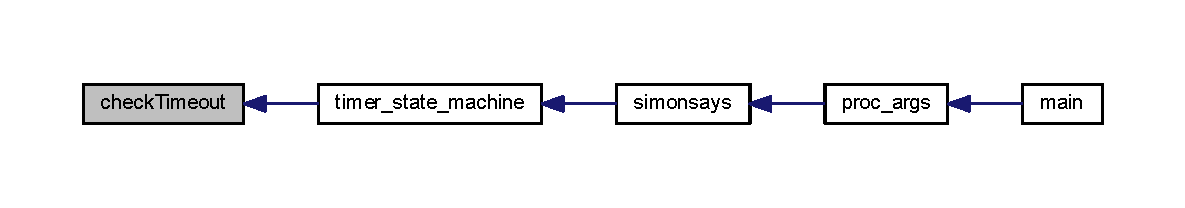
\includegraphics[width=350pt]{game_8c_a7bd272e601a5455dea734c829bf0feb4_icgraph}
\end{center}
\end{figure}
\mbox{\Hypertarget{game_8c_acee4b53c87749506d4f93ed0bdd32ccb}\label{game_8c_acee4b53c87749506d4f93ed0bdd32ccb}} 
\index{game.\+c@{game.\+c}!compare\+\_\+arrays@{compare\+\_\+arrays}}
\index{compare\+\_\+arrays@{compare\+\_\+arrays}!game.\+c@{game.\+c}}
\subsubsection{\texorpdfstring{compare\+\_\+arrays()}{compare\_arrays()}}
{\footnotesize\ttfamily int compare\+\_\+arrays (\begin{DoxyParamCaption}\item[{int $\ast$}]{array1,  }\item[{int $\ast$}]{array2,  }\item[{int}]{size }\end{DoxyParamCaption})}



compares the first size positions of two arrays 

if the first size positions are equal, then we consider both arrays equal


\begin{DoxyParams}{Parameters}
{\em array1} & first array to compare\\
\hline
{\em array2} & second array to compare\\
\hline
\end{DoxyParams}
number of position to be compared

\begin{DoxyReturn}{Returns}
Returns 1 the arrays are equal, returns zero otherwise 
\end{DoxyReturn}
Here is the caller graph for this function\+:\nopagebreak
\begin{figure}[H]
\begin{center}
\leavevmode
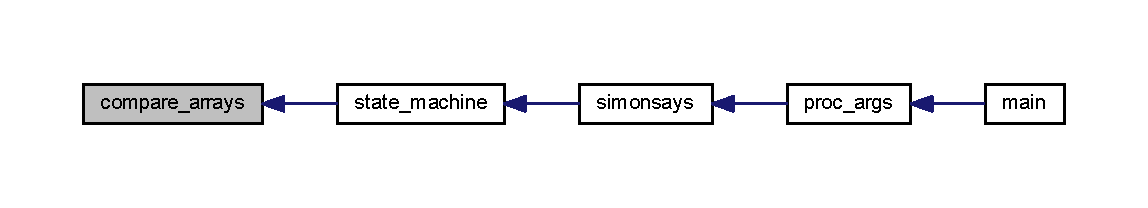
\includegraphics[width=350pt]{game_8c_acee4b53c87749506d4f93ed0bdd32ccb_icgraph}
\end{center}
\end{figure}
\mbox{\Hypertarget{game_8c_a434350c0629d48af15132bd626ff0e7b}\label{game_8c_a434350c0629d48af15132bd626ff0e7b}} 
\index{game.\+c@{game.\+c}!simonsays@{simonsays}}
\index{simonsays@{simonsays}!game.\+c@{game.\+c}}
\subsubsection{\texorpdfstring{simonsays()}{simonsays()}}
{\footnotesize\ttfamily int simonsays (\begin{DoxyParamCaption}{ }\end{DoxyParamCaption})}



main function that calls the game interruption handlers and the game state machine funtions 

Here is the call graph for this function\+:\nopagebreak
\begin{figure}[H]
\begin{center}
\leavevmode
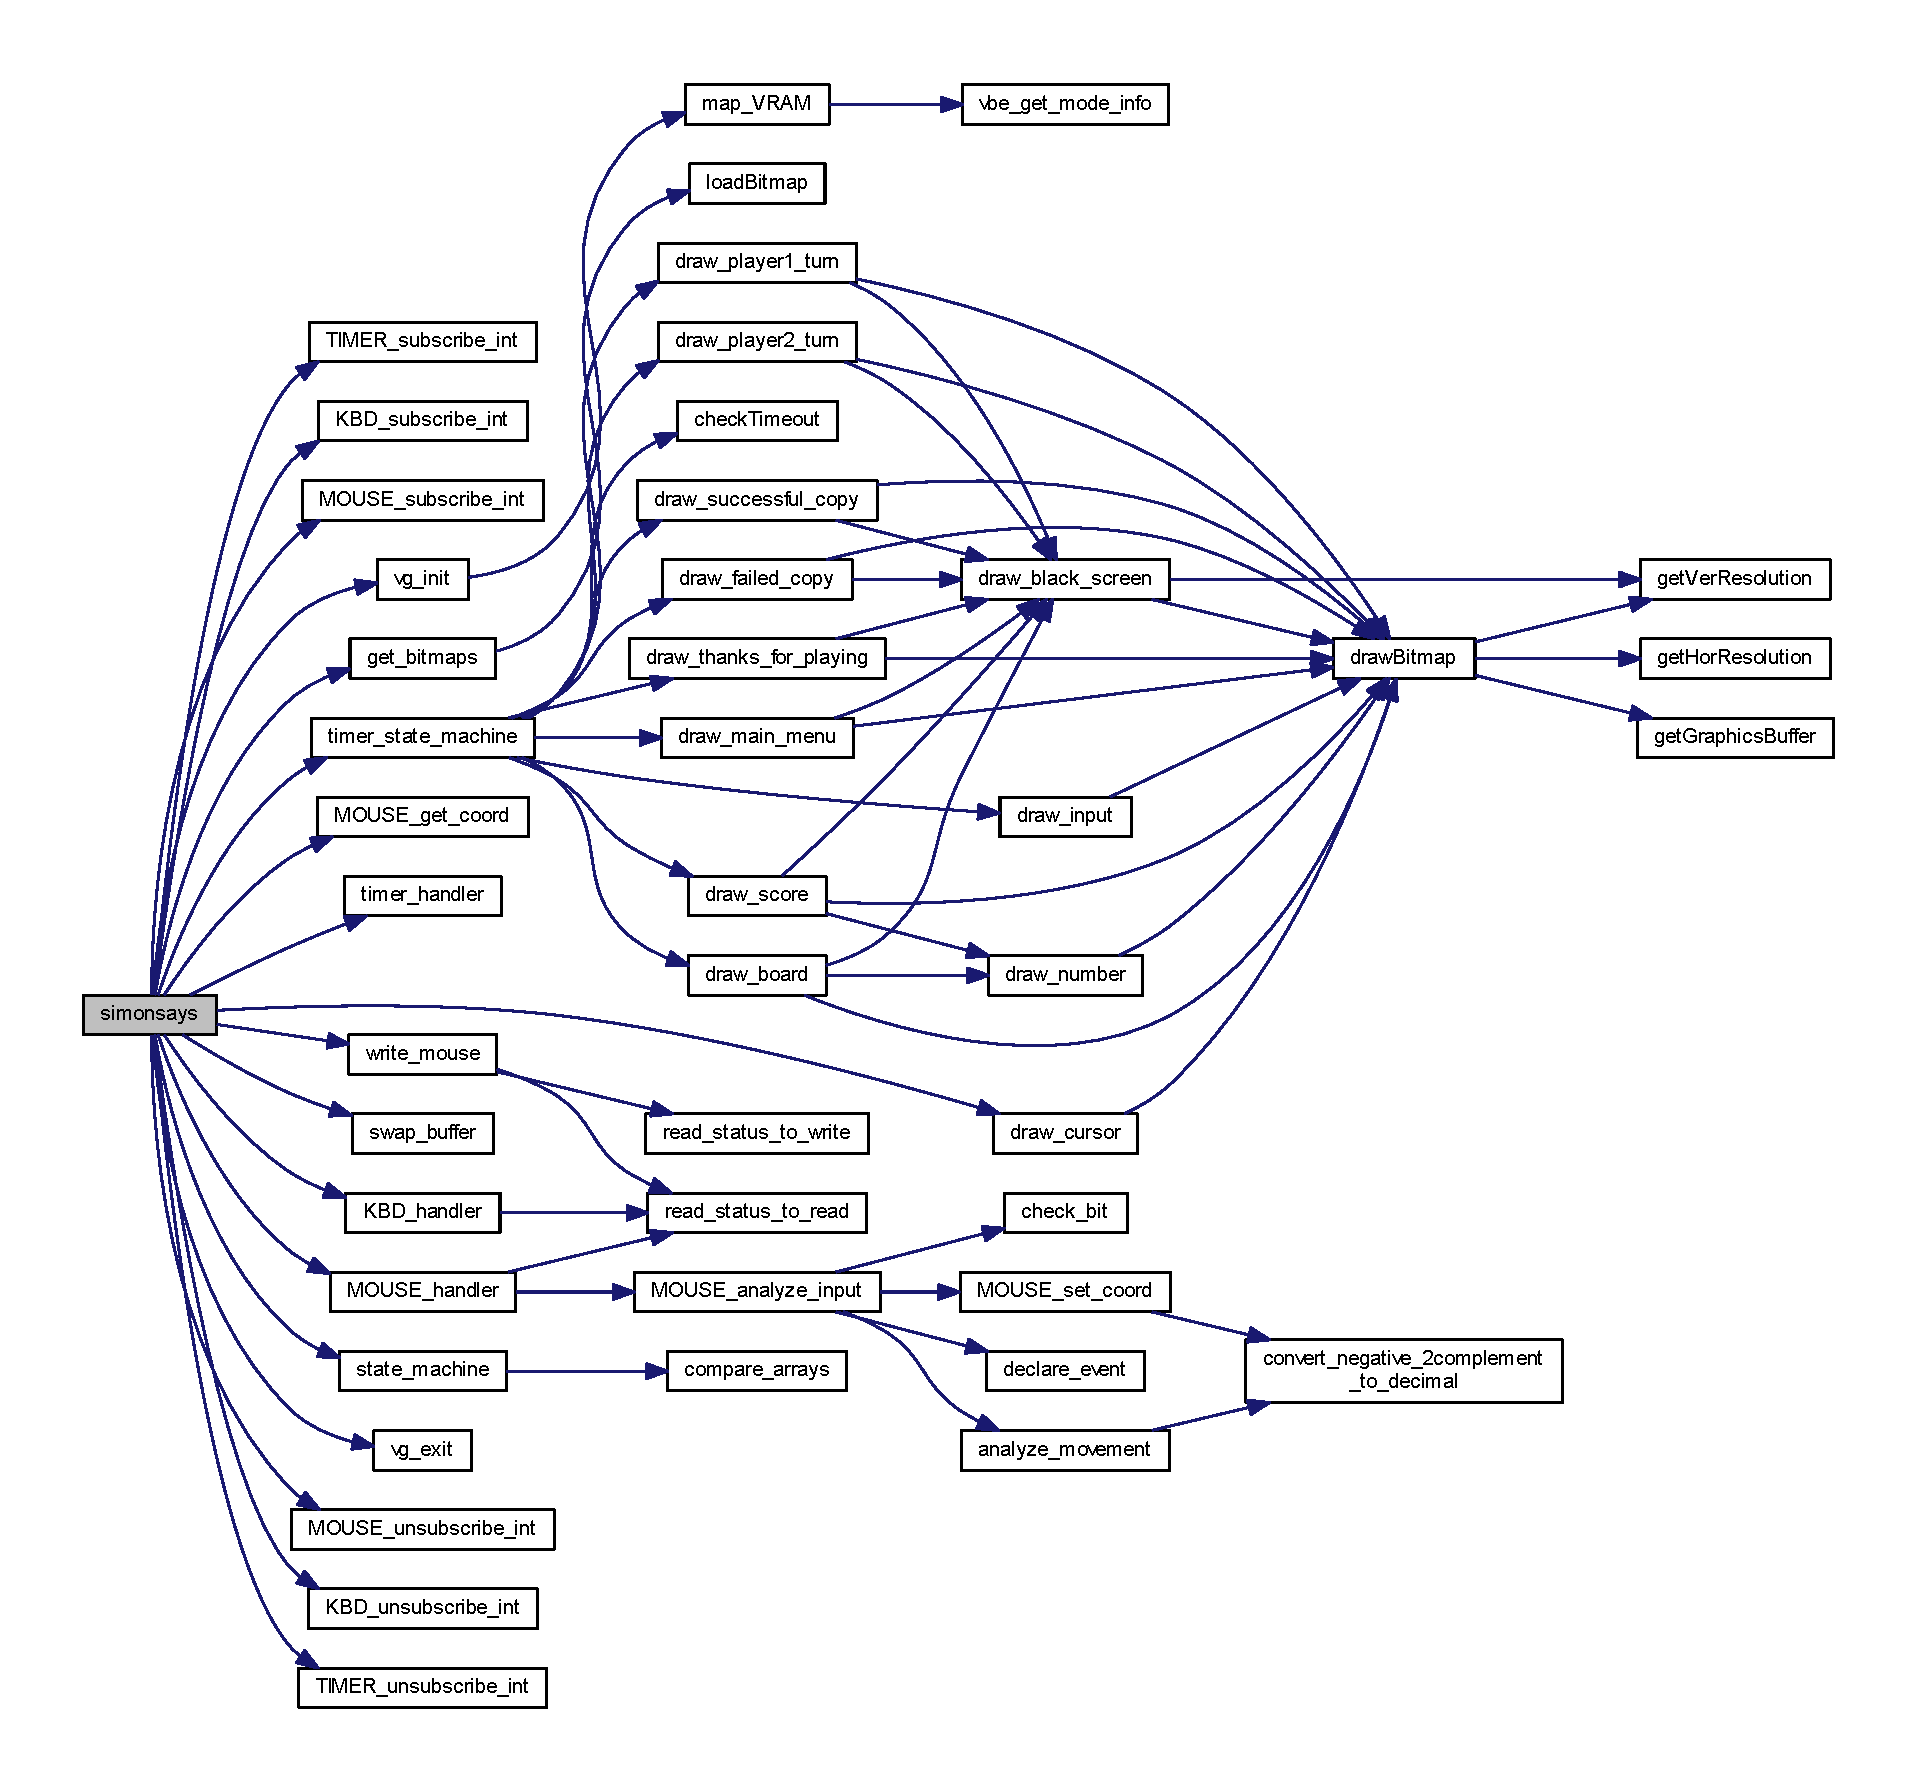
\includegraphics[width=350pt]{game_8c_a434350c0629d48af15132bd626ff0e7b_cgraph}
\end{center}
\end{figure}
Here is the caller graph for this function\+:\nopagebreak
\begin{figure}[H]
\begin{center}
\leavevmode
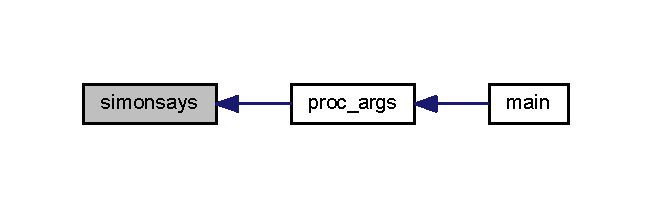
\includegraphics[width=313pt]{game_8c_a434350c0629d48af15132bd626ff0e7b_icgraph}
\end{center}
\end{figure}
\mbox{\Hypertarget{game_8c_a8101733e49b7935d3b1b8d2bb83dd42f}\label{game_8c_a8101733e49b7935d3b1b8d2bb83dd42f}} 
\index{game.\+c@{game.\+c}!state\+\_\+machine@{state\+\_\+machine}}
\index{state\+\_\+machine@{state\+\_\+machine}!game.\+c@{game.\+c}}
\subsubsection{\texorpdfstring{state\+\_\+machine()}{state\_machine()}}
{\footnotesize\ttfamily void state\+\_\+machine (\begin{DoxyParamCaption}\item[{int}]{input }\end{DoxyParamCaption})}



state machine that changes the game state according to the inputs given by the players 

This function is responsible for filling the arrays with the player inputs

This function also changes the state acording to the button pressed on the main menu(\+S\+T\+A\+R\+T O\+R E\+X\+I\+T)


\begin{DoxyParams}{Parameters}
{\em input} & input given by a player \\
\hline
\end{DoxyParams}
Here is the call graph for this function\+:\nopagebreak
\begin{figure}[H]
\begin{center}
\leavevmode
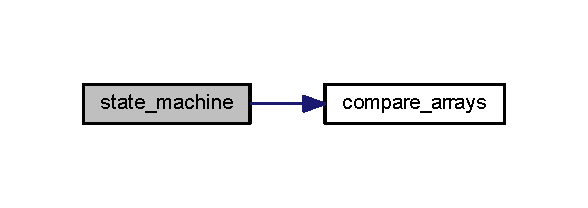
\includegraphics[width=282pt]{game_8c_a8101733e49b7935d3b1b8d2bb83dd42f_cgraph}
\end{center}
\end{figure}
Here is the caller graph for this function\+:\nopagebreak
\begin{figure}[H]
\begin{center}
\leavevmode
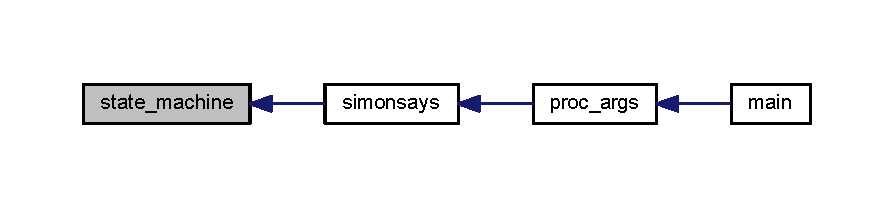
\includegraphics[width=350pt]{game_8c_a8101733e49b7935d3b1b8d2bb83dd42f_icgraph}
\end{center}
\end{figure}
\mbox{\Hypertarget{game_8c_a0ba54f993c5072ccad6ef0562e36443b}\label{game_8c_a0ba54f993c5072ccad6ef0562e36443b}} 
\index{game.\+c@{game.\+c}!timer\+\_\+state\+\_\+machine@{timer\+\_\+state\+\_\+machine}}
\index{timer\+\_\+state\+\_\+machine@{timer\+\_\+state\+\_\+machine}!game.\+c@{game.\+c}}
\subsubsection{\texorpdfstring{timer\+\_\+state\+\_\+machine()}{timer\_state\_machine()}}
{\footnotesize\ttfamily int timer\+\_\+state\+\_\+machine (\begin{DoxyParamCaption}\item[{int}]{input }\end{DoxyParamCaption})}



state machine that changes the game state according to the inputs given by the players ,makes the time pauses and draws the screen according to the current state 

although it has the same states as the state machine, the timer state machine is also responsible for the time pauses.


\begin{DoxyParams}{Parameters}
{\em input} & input given by a player\\
\hline
\end{DoxyParams}
\begin{DoxyReturn}{Returns}
Returns 1 if a timeout has started(only returns 1 in the beggining of the timeout, if we are in the middle of the timeout it returns 0), returns zero otherwise 
\end{DoxyReturn}
Here is the call graph for this function\+:\nopagebreak
\begin{figure}[H]
\begin{center}
\leavevmode
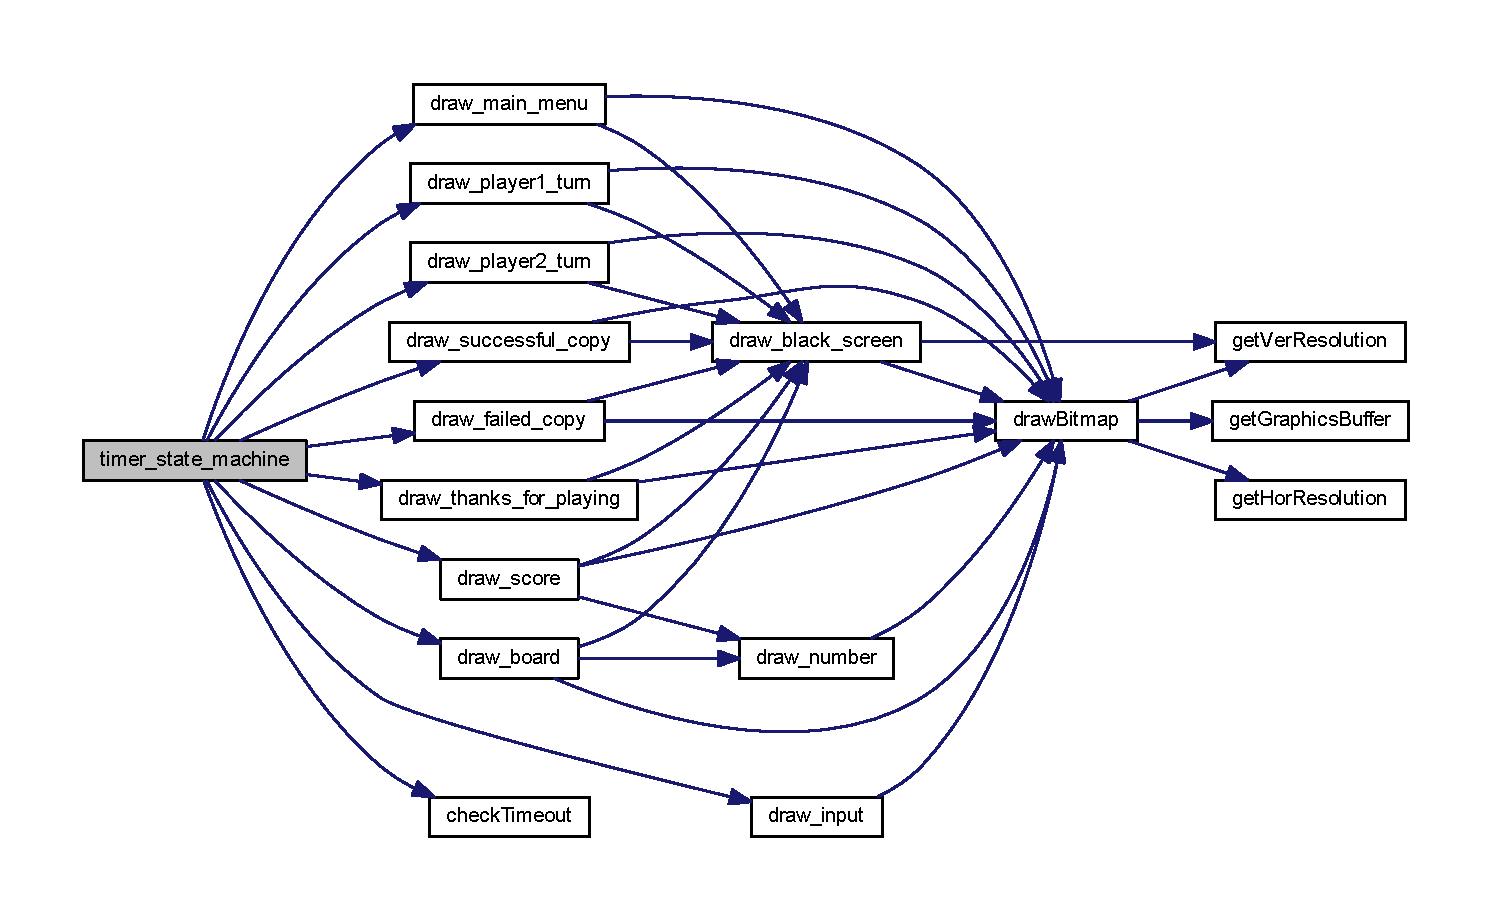
\includegraphics[width=350pt]{game_8c_a0ba54f993c5072ccad6ef0562e36443b_cgraph}
\end{center}
\end{figure}
Here is the caller graph for this function\+:\nopagebreak
\begin{figure}[H]
\begin{center}
\leavevmode
\includegraphics[width=350pt]{game_8c_a0ba54f993c5072ccad6ef0562e36443b_icgraph}
\end{center}
\end{figure}


\subsection{Variable Documentation}
\mbox{\Hypertarget{game_8c_acf78d5ab53d26add4184578b9732a6a0}\label{game_8c_acf78d5ab53d26add4184578b9732a6a0}} 
\index{game.\+c@{game.\+c}!escape@{escape}}
\index{escape@{escape}!game.\+c@{game.\+c}}
\subsubsection{\texorpdfstring{escape}{escape}}
{\footnotesize\ttfamily int escape = 0\hspace{0.3cm}{\ttfamily [static]}}

\mbox{\Hypertarget{game_8c_aed766d1a38b70be51df494da921471fa}\label{game_8c_aed766d1a38b70be51df494da921471fa}} 
\index{game.\+c@{game.\+c}!game\+\_\+state@{game\+\_\+state}}
\index{game\+\_\+state@{game\+\_\+state}!game.\+c@{game.\+c}}
\subsubsection{\texorpdfstring{game\+\_\+state}{game\_state}}
{\footnotesize\ttfamily \hyperlink{gamevariables_8h_a4edce1ca040716922b6e4a79be4e414d}{game\+\_\+state\+\_\+t} game\+\_\+state = \hyperlink{gamevariables_8h_a4edce1ca040716922b6e4a79be4e414dac22743f1fc74de09544ecc9bab74a17b}{M\+A\+I\+N\+\_\+\+M\+E\+NU}}

\mbox{\Hypertarget{game_8c_a9f96e639d82878ed2a43b4d80b45f626}\label{game_8c_a9f96e639d82878ed2a43b4d80b45f626}} 
\index{game.\+c@{game.\+c}!game\+\_\+turn@{game\+\_\+turn}}
\index{game\+\_\+turn@{game\+\_\+turn}!game.\+c@{game.\+c}}
\subsubsection{\texorpdfstring{game\+\_\+turn}{game\_turn}}
{\footnotesize\ttfamily \hyperlink{gamevariables_8h_a0a4ccc23c2081d8587459bfbe0bbeee4}{game\+\_\+turn\+\_\+t} game\+\_\+turn = \hyperlink{gamevariables_8h_a0a4ccc23c2081d8587459bfbe0bbeee4a77d1b58e26a2a3d61ce38e09764cbc19}{P\+L\+A\+Y\+E\+R1}}

\mbox{\Hypertarget{game_8c_ab2623c3ab961285567b984a662aa0a26}\label{game_8c_ab2623c3ab961285567b984a662aa0a26}} 
\index{game.\+c@{game.\+c}!mouse\+\_\+x\+\_\+coord@{mouse\+\_\+x\+\_\+coord}}
\index{mouse\+\_\+x\+\_\+coord@{mouse\+\_\+x\+\_\+coord}!game.\+c@{game.\+c}}
\subsubsection{\texorpdfstring{mouse\+\_\+x\+\_\+coord}{mouse\_x\_coord}}
{\footnotesize\ttfamily int mouse\+\_\+x\+\_\+coord\hspace{0.3cm}{\ttfamily [static]}}

\mbox{\Hypertarget{game_8c_aadada65942cf173e32057ab132f6be0c}\label{game_8c_aadada65942cf173e32057ab132f6be0c}} 
\index{game.\+c@{game.\+c}!mouse\+\_\+y\+\_\+coord@{mouse\+\_\+y\+\_\+coord}}
\index{mouse\+\_\+y\+\_\+coord@{mouse\+\_\+y\+\_\+coord}!game.\+c@{game.\+c}}
\subsubsection{\texorpdfstring{mouse\+\_\+y\+\_\+coord}{mouse\_y\_coord}}
{\footnotesize\ttfamily int mouse\+\_\+y\+\_\+coord\hspace{0.3cm}{\ttfamily [static]}}

\mbox{\Hypertarget{game_8c_a0d7ec96959b5e2328cb30a4a7e7dda10}\label{game_8c_a0d7ec96959b5e2328cb30a4a7e7dda10}} 
\index{game.\+c@{game.\+c}!player1\+\_\+array@{player1\+\_\+array}}
\index{player1\+\_\+array@{player1\+\_\+array}!game.\+c@{game.\+c}}
\subsubsection{\texorpdfstring{player1\+\_\+array}{player1\_array}}
{\footnotesize\ttfamily int player1\+\_\+array\mbox{[}10\mbox{]}\hspace{0.3cm}{\ttfamily [static]}}

\mbox{\Hypertarget{game_8c_a08cc02a3fdfc39ca7dce0da405d46872}\label{game_8c_a08cc02a3fdfc39ca7dce0da405d46872}} 
\index{game.\+c@{game.\+c}!player2\+\_\+array@{player2\+\_\+array}}
\index{player2\+\_\+array@{player2\+\_\+array}!game.\+c@{game.\+c}}
\subsubsection{\texorpdfstring{player2\+\_\+array}{player2\_array}}
{\footnotesize\ttfamily int player2\+\_\+array\mbox{[}10\mbox{]}\hspace{0.3cm}{\ttfamily [static]}}

\mbox{\Hypertarget{game_8c_a312bc2c706f64a3ba78f54cad26d9402}\label{game_8c_a312bc2c706f64a3ba78f54cad26d9402}} 
\index{game.\+c@{game.\+c}!player2\+\_\+score@{player2\+\_\+score}}
\index{player2\+\_\+score@{player2\+\_\+score}!game.\+c@{game.\+c}}
\subsubsection{\texorpdfstring{player2\+\_\+score}{player2\_score}}
{\footnotesize\ttfamily int player2\+\_\+score =0\hspace{0.3cm}{\ttfamily [static]}}

\mbox{\Hypertarget{game_8c_a828d22214652902b5071899608fb1169}\label{game_8c_a828d22214652902b5071899608fb1169}} 
\index{game.\+c@{game.\+c}!player\+\_\+state@{player\+\_\+state}}
\index{player\+\_\+state@{player\+\_\+state}!game.\+c@{game.\+c}}
\subsubsection{\texorpdfstring{player\+\_\+state}{player\_state}}
{\footnotesize\ttfamily \hyperlink{gamevariables_8h_a2282a264f9691d1742756ac5e4929238}{player\+\_\+state\+\_\+t} player\+\_\+state = \hyperlink{gamevariables_8h_a2282a264f9691d1742756ac5e4929238a88ec7d5086d2469ba843c7fcceade8a6}{D\+E\+F\+A\+U\+LT}}

\mbox{\Hypertarget{game_8c_a401e942526aac47cef94f478182486e7}\label{game_8c_a401e942526aac47cef94f478182486e7}} 
\index{game.\+c@{game.\+c}!position@{position}}
\index{position@{position}!game.\+c@{game.\+c}}
\subsubsection{\texorpdfstring{position}{position}}
{\footnotesize\ttfamily int position =0\hspace{0.3cm}{\ttfamily [static]}}

\mbox{\Hypertarget{game_8c_a0b7685156d686874cf7a3f95a6b7f3f3}\label{game_8c_a0b7685156d686874cf7a3f95a6b7f3f3}} 
\index{game.\+c@{game.\+c}!round@{round}}
\index{round@{round}!game.\+c@{game.\+c}}
\subsubsection{\texorpdfstring{round}{round}}
{\footnotesize\ttfamily unsigned int round = 1\hspace{0.3cm}{\ttfamily [static]}}

\mbox{\Hypertarget{game_8c_a83e57ce9bd59cfa0995c2e2c8589c274}\label{game_8c_a83e57ce9bd59cfa0995c2e2c8589c274}} 
\index{game.\+c@{game.\+c}!time@{time}}
\index{time@{time}!game.\+c@{game.\+c}}
\subsubsection{\texorpdfstring{time}{time}}
{\footnotesize\ttfamily unsigned int time = 0\hspace{0.3cm}{\ttfamily [static]}}

\mbox{\Hypertarget{game_8c_a493b57f443cc38b3d3df9c1e584d9d82}\label{game_8c_a493b57f443cc38b3d3df9c1e584d9d82}} 
\index{game.\+c@{game.\+c}!timeout@{timeout}}
\index{timeout@{timeout}!game.\+c@{game.\+c}}
\subsubsection{\texorpdfstring{timeout}{timeout}}
{\footnotesize\ttfamily int timeout =0\hspace{0.3cm}{\ttfamily [static]}}

\mbox{\Hypertarget{game_8c_a50f7ef6ef3124abc70fbd30e6c5f06ce}\label{game_8c_a50f7ef6ef3124abc70fbd30e6c5f06ce}} 
\index{game.\+c@{game.\+c}!timeout\+\_\+entered@{timeout\+\_\+entered}}
\index{timeout\+\_\+entered@{timeout\+\_\+entered}!game.\+c@{game.\+c}}
\subsubsection{\texorpdfstring{timeout\+\_\+entered}{timeout\_entered}}
{\footnotesize\ttfamily int timeout\+\_\+entered =0\hspace{0.3cm}{\ttfamily [static]}}

\mbox{\Hypertarget{game_8c_a4c5da45addccd0b2a643a6b73c2f3214}\label{game_8c_a4c5da45addccd0b2a643a6b73c2f3214}} 
\index{game.\+c@{game.\+c}!timeout\+\_\+started@{timeout\+\_\+started}}
\index{timeout\+\_\+started@{timeout\+\_\+started}!game.\+c@{game.\+c}}
\subsubsection{\texorpdfstring{timeout\+\_\+started}{timeout\_started}}
{\footnotesize\ttfamily int timeout\+\_\+started =0\hspace{0.3cm}{\ttfamily [static]}}

\mbox{\Hypertarget{game_8c_ab54283a672f4b80136585c9973814206}\label{game_8c_ab54283a672f4b80136585c9973814206}} 
\index{game.\+c@{game.\+c}!timer\+\_\+counter@{timer\+\_\+counter}}
\index{timer\+\_\+counter@{timer\+\_\+counter}!game.\+c@{game.\+c}}
\subsubsection{\texorpdfstring{timer\+\_\+counter}{timer\_counter}}
{\footnotesize\ttfamily unsigned int timer\+\_\+counter =0\hspace{0.3cm}{\ttfamily [static]}}


\hypertarget{game_8h}{}\section{C\+:/\+Users/\+Nelson/\+Desktop/\+L\+C\+OM -\/ 2ºano -\/ 2º semestre/source/game.h File Reference}
\label{game_8h}\index{C\+:/\+Users/\+Nelson/\+Desktop/\+L\+C\+O\+M -\/ 2ºano -\/ 2º semestre/source/game.\+h@{C\+:/\+Users/\+Nelson/\+Desktop/\+L\+C\+O\+M -\/ 2ºano -\/ 2º semestre/source/game.\+h}}
{\ttfamily \#include \char`\"{}keyboard.\+h\char`\"{}}\newline
{\ttfamily \#include \char`\"{}timer.\+h\char`\"{}}\newline
{\ttfamily \#include \char`\"{}video\+\_\+gr.\+h\char`\"{}}\newline
{\ttfamily \#include \char`\"{}vbe.\+h\char`\"{}}\newline
{\ttfamily \#include \char`\"{}mouse.\+h\char`\"{}}\newline
{\ttfamily \#include \char`\"{}gamevariables.\+h\char`\"{}}\newline
Include dependency graph for game.\+h\+:
\nopagebreak
\begin{figure}[H]
\begin{center}
\leavevmode
\includegraphics[width=350pt]{game_8h__incl}
\end{center}
\end{figure}
This graph shows which files directly or indirectly include this file\+:
\nopagebreak
\begin{figure}[H]
\begin{center}
\leavevmode
\includegraphics[width=350pt]{game_8h__dep__incl}
\end{center}
\end{figure}
\subsection*{Functions}
\begin{DoxyCompactItemize}
\item 
int \hyperlink{game_8h_a434350c0629d48af15132bd626ff0e7b}{simonsays} ()
\begin{DoxyCompactList}\small\item\em main function that calls the game interruption handlers and the game state machine funtions \end{DoxyCompactList}\item 
void \hyperlink{game_8h_a8101733e49b7935d3b1b8d2bb83dd42f}{state\+\_\+machine} (int input)
\begin{DoxyCompactList}\small\item\em state machine that changes the game state according to the inputs given by the players \end{DoxyCompactList}\item 
int \hyperlink{game_8h_a0ba54f993c5072ccad6ef0562e36443b}{timer\+\_\+state\+\_\+machine} (int input)
\begin{DoxyCompactList}\small\item\em state machine that changes the game state according to the inputs given by the players ,makes the time pauses and draws the screen according to the current state \end{DoxyCompactList}\item 
int \hyperlink{game_8h_a7bd272e601a5455dea734c829bf0feb4}{check\+Timeout} (int pause\+\_\+time)
\begin{DoxyCompactList}\small\item\em is used to make a timeout(wait a number of seconds without doing anything) \end{DoxyCompactList}\item 
int \hyperlink{game_8h_acee4b53c87749506d4f93ed0bdd32ccb}{compare\+\_\+arrays} (int $\ast$array1, int $\ast$array2, int size)
\begin{DoxyCompactList}\small\item\em compares the first size positions of two arrays \end{DoxyCompactList}\end{DoxyCompactItemize}


\subsection{Function Documentation}
\mbox{\Hypertarget{game_8h_a7bd272e601a5455dea734c829bf0feb4}\label{game_8h_a7bd272e601a5455dea734c829bf0feb4}} 
\index{game.\+h@{game.\+h}!check\+Timeout@{check\+Timeout}}
\index{check\+Timeout@{check\+Timeout}!game.\+h@{game.\+h}}
\subsubsection{\texorpdfstring{check\+Timeout()}{checkTimeout()}}
{\footnotesize\ttfamily int check\+Timeout (\begin{DoxyParamCaption}\item[{int}]{pause\+\_\+time }\end{DoxyParamCaption})}



is used to make a timeout(wait a number of seconds without doing anything) 

is useful between turns and other cases


\begin{DoxyParams}{Parameters}
{\em pause\+\_\+time} & indicates the timeout number of seconds\\
\hline
\end{DoxyParams}
\begin{DoxyReturn}{Returns}
Returns 1 if a timeout has started(only returns 1 in the beggining of the timeout, if we are in the middle of the timeout it returns 0), returns zero otherwise 
\end{DoxyReturn}
Here is the caller graph for this function\+:\nopagebreak
\begin{figure}[H]
\begin{center}
\leavevmode
\includegraphics[width=350pt]{game_8h_a7bd272e601a5455dea734c829bf0feb4_icgraph}
\end{center}
\end{figure}
\mbox{\Hypertarget{game_8h_acee4b53c87749506d4f93ed0bdd32ccb}\label{game_8h_acee4b53c87749506d4f93ed0bdd32ccb}} 
\index{game.\+h@{game.\+h}!compare\+\_\+arrays@{compare\+\_\+arrays}}
\index{compare\+\_\+arrays@{compare\+\_\+arrays}!game.\+h@{game.\+h}}
\subsubsection{\texorpdfstring{compare\+\_\+arrays()}{compare\_arrays()}}
{\footnotesize\ttfamily int compare\+\_\+arrays (\begin{DoxyParamCaption}\item[{int $\ast$}]{array1,  }\item[{int $\ast$}]{array2,  }\item[{int}]{size }\end{DoxyParamCaption})}



compares the first size positions of two arrays 

if the first size positions are equal, then we consider both arrays equal


\begin{DoxyParams}{Parameters}
{\em array1} & first array to compare\\
\hline
{\em array2} & second array to compare\\
\hline
\end{DoxyParams}
number of position to be compared

\begin{DoxyReturn}{Returns}
Returns 1 the arrays are equal, returns zero otherwise 
\end{DoxyReturn}
Here is the caller graph for this function\+:\nopagebreak
\begin{figure}[H]
\begin{center}
\leavevmode
\includegraphics[width=350pt]{game_8h_acee4b53c87749506d4f93ed0bdd32ccb_icgraph}
\end{center}
\end{figure}
\mbox{\Hypertarget{game_8h_a434350c0629d48af15132bd626ff0e7b}\label{game_8h_a434350c0629d48af15132bd626ff0e7b}} 
\index{game.\+h@{game.\+h}!simonsays@{simonsays}}
\index{simonsays@{simonsays}!game.\+h@{game.\+h}}
\subsubsection{\texorpdfstring{simonsays()}{simonsays()}}
{\footnotesize\ttfamily int simonsays (\begin{DoxyParamCaption}{ }\end{DoxyParamCaption})}



main function that calls the game interruption handlers and the game state machine funtions 

Here is the call graph for this function\+:\nopagebreak
\begin{figure}[H]
\begin{center}
\leavevmode
\includegraphics[width=350pt]{game_8h_a434350c0629d48af15132bd626ff0e7b_cgraph}
\end{center}
\end{figure}
Here is the caller graph for this function\+:\nopagebreak
\begin{figure}[H]
\begin{center}
\leavevmode
\includegraphics[width=313pt]{game_8h_a434350c0629d48af15132bd626ff0e7b_icgraph}
\end{center}
\end{figure}
\mbox{\Hypertarget{game_8h_a8101733e49b7935d3b1b8d2bb83dd42f}\label{game_8h_a8101733e49b7935d3b1b8d2bb83dd42f}} 
\index{game.\+h@{game.\+h}!state\+\_\+machine@{state\+\_\+machine}}
\index{state\+\_\+machine@{state\+\_\+machine}!game.\+h@{game.\+h}}
\subsubsection{\texorpdfstring{state\+\_\+machine()}{state\_machine()}}
{\footnotesize\ttfamily void state\+\_\+machine (\begin{DoxyParamCaption}\item[{int}]{input }\end{DoxyParamCaption})}



state machine that changes the game state according to the inputs given by the players 

This function is responsible for filling the arrays with the player inputs

This function also changes the state acording to the button pressed on the main menu(\+S\+T\+A\+R\+T O\+R E\+X\+I\+T)


\begin{DoxyParams}{Parameters}
{\em input} & input given by a player \\
\hline
\end{DoxyParams}
Here is the call graph for this function\+:\nopagebreak
\begin{figure}[H]
\begin{center}
\leavevmode
\includegraphics[width=282pt]{game_8h_a8101733e49b7935d3b1b8d2bb83dd42f_cgraph}
\end{center}
\end{figure}
Here is the caller graph for this function\+:\nopagebreak
\begin{figure}[H]
\begin{center}
\leavevmode
\includegraphics[width=350pt]{game_8h_a8101733e49b7935d3b1b8d2bb83dd42f_icgraph}
\end{center}
\end{figure}
\mbox{\Hypertarget{game_8h_a0ba54f993c5072ccad6ef0562e36443b}\label{game_8h_a0ba54f993c5072ccad6ef0562e36443b}} 
\index{game.\+h@{game.\+h}!timer\+\_\+state\+\_\+machine@{timer\+\_\+state\+\_\+machine}}
\index{timer\+\_\+state\+\_\+machine@{timer\+\_\+state\+\_\+machine}!game.\+h@{game.\+h}}
\subsubsection{\texorpdfstring{timer\+\_\+state\+\_\+machine()}{timer\_state\_machine()}}
{\footnotesize\ttfamily int timer\+\_\+state\+\_\+machine (\begin{DoxyParamCaption}\item[{int}]{input }\end{DoxyParamCaption})}



state machine that changes the game state according to the inputs given by the players ,makes the time pauses and draws the screen according to the current state 

although it has the same states as the state machine, the timer state machine is also responsible for the time pauses.


\begin{DoxyParams}{Parameters}
{\em input} & input given by a player\\
\hline
\end{DoxyParams}
\begin{DoxyReturn}{Returns}
Returns 1 if a timeout has started(only returns 1 in the beggining of the timeout, if we are in the middle of the timeout it returns 0), returns zero otherwise 
\end{DoxyReturn}
Here is the call graph for this function\+:\nopagebreak
\begin{figure}[H]
\begin{center}
\leavevmode
\includegraphics[width=350pt]{game_8h_a0ba54f993c5072ccad6ef0562e36443b_cgraph}
\end{center}
\end{figure}
Here is the caller graph for this function\+:\nopagebreak
\begin{figure}[H]
\begin{center}
\leavevmode
\includegraphics[width=350pt]{game_8h_a0ba54f993c5072ccad6ef0562e36443b_icgraph}
\end{center}
\end{figure}

\hypertarget{gamevariables_8h}{}\section{C\+:/\+Users/\+Nelson/\+Desktop/\+L\+C\+OM -\/ 2ºano -\/ 2º semestre/source/gamevariables.h File Reference}
\label{gamevariables_8h}\index{C\+:/\+Users/\+Nelson/\+Desktop/\+L\+C\+O\+M -\/ 2ºano -\/ 2º semestre/source/gamevariables.\+h@{C\+:/\+Users/\+Nelson/\+Desktop/\+L\+C\+O\+M -\/ 2ºano -\/ 2º semestre/source/gamevariables.\+h}}
This graph shows which files directly or indirectly include this file\+:
\nopagebreak
\begin{figure}[H]
\begin{center}
\leavevmode
\includegraphics[width=350pt]{gamevariables_8h__dep__incl}
\end{center}
\end{figure}
\subsection*{Macros}
\begin{DoxyCompactItemize}
\item 
\#define \hyperlink{gamevariables_8h_a1d8df6fec341be5008a9291378327a59}{I\+N\+V\+A\+L\+I\+D\+\_\+\+I\+N\+P\+UT}~0
\begin{DoxyCompactList}\small\item\em Represents a player move(input) that is not accepted by the game. \end{DoxyCompactList}\item 
\#define \hyperlink{gamevariables_8h_a9b4f59fc9220530978f12905fe51b1d0}{E\+S\+C\+\_\+\+K\+EY}~1
\begin{DoxyCompactList}\small\item\em Represents the escape key input. \end{DoxyCompactList}\item 
\#define \hyperlink{gamevariables_8h_a2e092124f706e9898a26f3d0c6dd33d3}{A\+\_\+\+K\+EY}~2
\begin{DoxyCompactList}\small\item\em Represents the A key input. \end{DoxyCompactList}\item 
\#define \hyperlink{gamevariables_8h_a8cb726577cd35fc0582744b2270e192f}{W\+\_\+\+K\+EY}~3
\begin{DoxyCompactList}\small\item\em Represents the W key input. \end{DoxyCompactList}\item 
\#define \hyperlink{gamevariables_8h_a38916d959d471a2781d390910271b6b5}{S\+\_\+\+K\+EY}~4
\begin{DoxyCompactList}\small\item\em Represents the S key input. \end{DoxyCompactList}\item 
\#define \hyperlink{gamevariables_8h_a23c8dc1c6696b91ba6b96f2dca53b7ba}{D\+\_\+\+K\+EY}~5
\begin{DoxyCompactList}\small\item\em Represents the D key input. \end{DoxyCompactList}\item 
\#define \hyperlink{gamevariables_8h_af97853127c8cc9ad9180c05295c809b4}{T\+R\+I\+A\+N\+G\+LE}~6
\begin{DoxyCompactList}\small\item\em Represents the triangle input. \end{DoxyCompactList}\item 
\#define \hyperlink{gamevariables_8h_a4a49761654ff508d856c6c1b4d132442}{C\+I\+R\+C\+LE}~7
\begin{DoxyCompactList}\small\item\em Represents the circle input. \end{DoxyCompactList}\item 
\#define \hyperlink{gamevariables_8h_a94c3dc9846edbbb70f678768633a4796}{S\+T\+AR}~8
\begin{DoxyCompactList}\small\item\em Represents the star input. \end{DoxyCompactList}\item 
\#define \hyperlink{gamevariables_8h_afa81feaf17942c56aeb0624e27ddb647}{S\+Q\+U\+A\+RE}~9
\begin{DoxyCompactList}\small\item\em Represents the square input. \end{DoxyCompactList}\item 
\#define \hyperlink{gamevariables_8h_a1341f3eff06e67e6e9fc9768997fc842}{A\+S\+C\+E\+N\+D\+E\+N\+T\+\_\+\+S\+L\+O\+PE}~10
\begin{DoxyCompactList}\small\item\em Represents the ascend slope input. \end{DoxyCompactList}\item 
\#define \hyperlink{gamevariables_8h_a18bb7e6210f55dfb46dcb3be38743a04}{D\+E\+S\+C\+E\+N\+D\+E\+N\+T\+\_\+\+S\+L\+O\+PE}~11
\begin{DoxyCompactList}\small\item\em Represents the descendent slope input. \end{DoxyCompactList}\item 
\#define \hyperlink{gamevariables_8h_a77f1ae1eacd663bf85ae4f2ab4c5adc1}{S\+T\+A\+R\+T\+\_\+\+I\+N\+P\+UT}~20
\begin{DoxyCompactList}\small\item\em Represents the start button input on hte main menu. \end{DoxyCompactList}\item 
\#define \hyperlink{gamevariables_8h_a6731437accb466b2cab056e15fedf068}{E\+X\+I\+T\+\_\+\+I\+N\+P\+UT}~21
\begin{DoxyCompactList}\small\item\em Represents the exit button input on hte main menu. \end{DoxyCompactList}\item 
\#define \hyperlink{gamevariables_8h_ae131505929d266ec4603f41551684452}{L\+E\+F\+T\+\_\+\+C\+L\+I\+CK}~30
\begin{DoxyCompactList}\small\item\em Represents the mouse left button click. \end{DoxyCompactList}\item 
\#define \hyperlink{gamevariables_8h_a9f0a372d451b2307b1f1a872400878ae}{R\+I\+G\+H\+T\+\_\+\+C\+L\+I\+CK}~31
\begin{DoxyCompactList}\small\item\em Represents the mouse right button click. \end{DoxyCompactList}\item 
\#define \hyperlink{gamevariables_8h_ab322693572e4146b8e2de2736083a64c}{S\+Q\+U\+A\+R\+E\+\_\+\+L\+E\+F\+T\+\_\+\+B\+O\+R\+D\+ER}~65
\item 
\#define \hyperlink{gamevariables_8h_af37063dc931a8c8f8d4af106b12c835f}{S\+Q\+U\+A\+R\+E\+\_\+\+R\+I\+G\+H\+T\+\_\+\+B\+O\+R\+D\+ER}~193
\item 
\#define \hyperlink{gamevariables_8h_a6cb55335fb75b7389514d34b5ab301f9}{S\+Q\+U\+A\+R\+E\+\_\+\+T\+O\+P\+\_\+\+B\+O\+R\+D\+ER}~433
\item 
\#define \hyperlink{gamevariables_8h_ade6e18b2d0e227da8fc224587f7fb323}{S\+Q\+U\+A\+R\+E\+\_\+\+B\+O\+T\+T\+O\+M\+\_\+\+B\+O\+R\+D\+ER}~305
\item 
\#define \hyperlink{gamevariables_8h_a7a04fbaa56f7c56d46b08a89ffbdf46b}{T\+R\+I\+A\+N\+G\+L\+E\+\_\+\+L\+E\+F\+T\+\_\+\+B\+O\+R\+D\+ER}~210
\item 
\#define \hyperlink{gamevariables_8h_a18b248b8cb0e31b3b0c6793a5ffbaae1}{T\+R\+I\+A\+N\+G\+L\+E\+\_\+\+R\+I\+G\+H\+T\+\_\+\+B\+O\+R\+D\+ER}~338
\item 
\#define \hyperlink{gamevariables_8h_a31f6120834e657144beb41fc24120576}{T\+R\+I\+A\+N\+G\+L\+E\+\_\+\+T\+O\+P\+\_\+\+B\+O\+R\+D\+ER}~286
\item 
\#define \hyperlink{gamevariables_8h_ae65468e1a3a38b14eccfb5303667a9bb}{T\+R\+I\+A\+N\+G\+L\+E\+\_\+\+B\+O\+T\+T\+O\+M\+\_\+\+B\+O\+R\+D\+ER}~170
\item 
\#define \hyperlink{gamevariables_8h_acec0c96e976ae9451ce7ac8334d35249}{C\+I\+R\+C\+L\+E\+\_\+\+L\+E\+F\+T\+\_\+\+B\+O\+R\+D\+ER}~340
\item 
\#define \hyperlink{gamevariables_8h_a7084fd719ca042c2ce85806d013b1e55}{C\+I\+R\+C\+L\+E\+\_\+\+R\+I\+G\+H\+T\+\_\+\+B\+O\+R\+D\+ER}~470
\item 
\#define \hyperlink{gamevariables_8h_ac8f355425821faeed0ad6e3a9232d5d6}{C\+I\+R\+C\+L\+E\+\_\+\+T\+O\+P\+\_\+\+B\+O\+R\+D\+ER}~428
\item 
\#define \hyperlink{gamevariables_8h_a7aedbe60fe0b6605a9d2a803422d53ca}{C\+I\+R\+C\+L\+E\+\_\+\+B\+O\+T\+T\+O\+M\+\_\+\+B\+O\+R\+D\+ER}~300
\item 
\#define \hyperlink{gamevariables_8h_a62574850c332ce5bcb15f604f4c37162}{S\+T\+A\+R\+\_\+\+L\+E\+F\+T\+\_\+\+B\+O\+R\+D\+ER}~210
\item 
\#define \hyperlink{gamevariables_8h_a5534da4961d5cb7b8feba68a296f703b}{S\+T\+A\+R\+\_\+\+R\+I\+G\+H\+T\+\_\+\+B\+O\+R\+D\+ER}~344
\item 
\#define \hyperlink{gamevariables_8h_a7ae6a643fd0b5d7d785dbfd4293cabac}{S\+T\+A\+R\+\_\+\+T\+O\+P\+\_\+\+B\+O\+R\+D\+ER}~668
\item 
\#define \hyperlink{gamevariables_8h_aa140bd30a400b922739c29e657322785}{S\+T\+A\+R\+\_\+\+B\+O\+T\+T\+O\+M\+\_\+\+B\+O\+R\+D\+ER}~440
\item 
\#define \hyperlink{gamevariables_8h_a79b13b9fb0948fe505c697c4788a8edf}{S\+T\+A\+R\+T\+\_\+\+L\+E\+F\+T\+\_\+\+B\+O\+R\+D\+ER}~210
\item 
\#define \hyperlink{gamevariables_8h_aca1a4699ac53784de78dff7f621ffe88}{S\+T\+A\+R\+T\+\_\+\+R\+I\+G\+H\+T\+\_\+\+B\+O\+R\+D\+ER}~352
\item 
\#define \hyperlink{gamevariables_8h_a9f106d89798ea62f4cf01bb451231206}{S\+T\+A\+R\+T\+\_\+\+T\+O\+P\+\_\+\+B\+O\+R\+D\+ER}~567
\item 
\#define \hyperlink{gamevariables_8h_a8459f517bb2ce611de5973f5fec622c5}{S\+T\+A\+R\+T\+\_\+\+B\+O\+T\+T\+O\+M\+\_\+\+B\+O\+R\+D\+ER}~425
\item 
\#define \hyperlink{gamevariables_8h_a6d0acf4724afa0bd1c5bd7194771eb23}{E\+X\+I\+T\+\_\+\+L\+E\+F\+T\+\_\+\+B\+O\+R\+D\+ER}~450
\item 
\#define \hyperlink{gamevariables_8h_a22640614394ffb998660c95ef4b71b04}{E\+X\+I\+T\+\_\+\+R\+I\+G\+H\+T\+\_\+\+B\+O\+R\+D\+ER}~592
\item 
\#define \hyperlink{gamevariables_8h_a613571abb65473d38233ddf36c287478}{E\+X\+I\+T\+\_\+\+T\+O\+P\+\_\+\+B\+O\+R\+D\+ER}~567
\item 
\#define \hyperlink{gamevariables_8h_af58136eb8b00618d6a9b4d9f6a04a2fc}{E\+X\+I\+T\+\_\+\+B\+O\+T\+T\+O\+M\+\_\+\+B\+O\+R\+D\+ER}~425
\item 
\#define \hyperlink{gamevariables_8h_a30362161c93e3f1a4ee4c673f535b5a8}{L\+E\+N\+G\+TH}~300
\begin{DoxyCompactList}\small\item\em minimum length considered for the mouse vertical slope distance \end{DoxyCompactList}\item 
\#define \hyperlink{gamevariables_8h_a5de99031704f5a4356e8fb30d56c4986}{C\+U\+R\+S\+O\+R\+\_\+\+S\+P\+E\+ED}~1
\begin{DoxyCompactList}\small\item\em speed at wich the mouse animation will move when a positive slope has been made \end{DoxyCompactList}\item 
\#define \hyperlink{gamevariables_8h_af12256afccd961784a2836a992e81e68}{R\+O\+U\+N\+D\+\_\+\+L\+I\+M\+IT}~10
\begin{DoxyCompactList}\small\item\em number of rounds the game will last for \end{DoxyCompactList}\item 
\#define \hyperlink{gamevariables_8h_ae061150d2634778e5d0b48d1e780efd0}{I\+N\+P\+U\+T\+\_\+\+T\+I\+M\+E\+O\+UT}~2
\begin{DoxyCompactList}\small\item\em time to wait after a player has given an input, it is also the time for wich the input image will be on the screen \end{DoxyCompactList}\item 
\#define \hyperlink{gamevariables_8h_a7818545dc00d473bf9b99922923b44c0}{T\+U\+R\+N\+\_\+\+A\+N\+N\+O\+U\+N\+C\+E\+M\+E\+N\+T\+\_\+\+T\+I\+M\+E\+O\+UT}~3
\begin{DoxyCompactList}\small\item\em time that the player turn announcement image will last on the screen \end{DoxyCompactList}\item 
\#define \hyperlink{gamevariables_8h_aa7afe20bc16922e7576cc4bdfd0763ee}{R\+O\+U\+N\+D\+\_\+\+R\+E\+S\+U\+L\+T\+\_\+\+T\+I\+M\+E\+O\+UT}~3
\begin{DoxyCompactList}\small\item\em time that the player2\textquotesingle{}s round result(copied successfuly or not) image will last on the screen \end{DoxyCompactList}\item 
\#define \hyperlink{gamevariables_8h_a932e2875b9cdfb3a987f3548eece5510}{F\+I\+N\+A\+L\+\_\+\+S\+C\+O\+R\+E\+\_\+\+T\+I\+M\+E\+O\+UT}~5
\begin{DoxyCompactList}\small\item\em time that the player2\textquotesingle{}s game final score image will last on the screen \end{DoxyCompactList}\item 
\#define \hyperlink{gamevariables_8h_abe148ab51c99507e84fbc39d30c00acd}{T\+H\+A\+N\+K\+S\+\_\+\+T\+I\+M\+E\+O\+UT}~5
\begin{DoxyCompactList}\small\item\em time that the \char`\"{}thanks for playing\char`\"{} image will last on the screen \end{DoxyCompactList}\end{DoxyCompactItemize}
\subsection*{Enumerations}
\begin{DoxyCompactItemize}
\item 
enum \hyperlink{gamevariables_8h_a0a4ccc23c2081d8587459bfbe0bbeee4}{game\+\_\+turn\+\_\+t} \{ \hyperlink{gamevariables_8h_a0a4ccc23c2081d8587459bfbe0bbeee4a77d1b58e26a2a3d61ce38e09764cbc19}{P\+L\+A\+Y\+E\+R1}, 
\hyperlink{gamevariables_8h_a0a4ccc23c2081d8587459bfbe0bbeee4a32a327d66c65387bb124f6c9408ff90b}{P\+L\+A\+Y\+E\+R2}
 \}
\item 
enum \hyperlink{gamevariables_8h_a4edce1ca040716922b6e4a79be4e414d}{game\+\_\+state\+\_\+t} \{ \newline
\hyperlink{gamevariables_8h_a4edce1ca040716922b6e4a79be4e414dac22743f1fc74de09544ecc9bab74a17b}{M\+A\+I\+N\+\_\+\+M\+E\+NU}, 
\hyperlink{gamevariables_8h_a4edce1ca040716922b6e4a79be4e414da13d000b4d7dc70d90239b7430d1eb6b2}{S\+T\+A\+RT}, 
\hyperlink{gamevariables_8h_a4edce1ca040716922b6e4a79be4e414da319c3a9f3a686e18245f51318d3754d9}{T\+U\+R\+N\+\_\+\+T\+R\+A\+N\+S\+I\+T\+I\+ON}, 
\hyperlink{gamevariables_8h_a4edce1ca040716922b6e4a79be4e414da1d9cba60714679da3517ed34da79c275}{T\+U\+R\+N\+\_\+\+T\+R\+A\+N\+S\+I\+T\+I\+O\+N2}, 
\newline
\hyperlink{gamevariables_8h_a4edce1ca040716922b6e4a79be4e414daafd8617ad9fe5cfb445d8a5780498c61}{R\+O\+U\+N\+D\+\_\+\+T\+R\+A\+N\+S\+I\+T\+I\+ON}, 
\hyperlink{gamevariables_8h_a4edce1ca040716922b6e4a79be4e414da54fbabe9b226608d2cc545eef9d31f41}{R\+O\+U\+N\+D\+\_\+\+T\+R\+A\+N\+S\+I\+T\+I\+O\+N2}, 
\hyperlink{gamevariables_8h_a4edce1ca040716922b6e4a79be4e414dae310c909d76b003d016bef8bdf16936a}{I\+N\+P\+UT}, 
\hyperlink{gamevariables_8h_a4edce1ca040716922b6e4a79be4e414daf095245f5cebc27a97a124345269fed8}{P\+L\+A\+Y\+I\+NG}, 
\newline
\hyperlink{gamevariables_8h_a4edce1ca040716922b6e4a79be4e414daa269b19326a9ac6f88eb3e0282bbcab9}{P\+R\+E\+\_\+\+E\+N\+D\+I\+NG}, 
\hyperlink{gamevariables_8h_a4edce1ca040716922b6e4a79be4e414daca114391980a4b8e57873b25c0e16b75}{E\+N\+D\+I\+NG}, 
\hyperlink{gamevariables_8h_a4edce1ca040716922b6e4a79be4e414dafdcf5da1f385793bfab13089afc6db1c}{E\+N\+D\+\_\+\+G\+A\+ME}, 
\hyperlink{gamevariables_8h_a4edce1ca040716922b6e4a79be4e414da4bf4cbde18067e0600c7c8a7a30ba316}{E\+X\+I\+T\+\_\+\+G\+A\+ME}
 \}
\item 
enum \hyperlink{gamevariables_8h_a2282a264f9691d1742756ac5e4929238}{player\+\_\+state\+\_\+t} \{ \hyperlink{gamevariables_8h_a2282a264f9691d1742756ac5e4929238a88ec7d5086d2469ba843c7fcceade8a6}{D\+E\+F\+A\+U\+LT}, 
\hyperlink{gamevariables_8h_a2282a264f9691d1742756ac5e4929238a843dff91ff0b0e5b98a110a512b2f531}{W\+IN}, 
\hyperlink{gamevariables_8h_a2282a264f9691d1742756ac5e4929238aa3c6650b8f7e145f2e4f434f5912b995}{L\+O\+SE}
 \}
\end{DoxyCompactItemize}
\subsection*{Variables}
\begin{DoxyCompactItemize}
\item 
unsigned int \hyperlink{gamevariables_8h_af205dd77c714102d927af4789ce00de0}{X\+\_\+\+I\+M\+G\+\_\+\+C\+O\+O\+RD}
\begin{DoxyCompactList}\small\item\em x coordinate that a mouse animated image will take, this animated image will appear when a positive slope has been made with the mouse \end{DoxyCompactList}\item 
unsigned int \hyperlink{gamevariables_8h_abd72042a657b8d388d31a8f31c887557}{Y\+\_\+\+I\+M\+G\+\_\+\+C\+O\+O\+RD}
\begin{DoxyCompactList}\small\item\em y coordinate that a mouse animated image will take, this animated image will appear when a positive slope has been made with the mouse \end{DoxyCompactList}\end{DoxyCompactItemize}


\subsection{Macro Definition Documentation}
\mbox{\Hypertarget{gamevariables_8h_a2e092124f706e9898a26f3d0c6dd33d3}\label{gamevariables_8h_a2e092124f706e9898a26f3d0c6dd33d3}} 
\index{gamevariables.\+h@{gamevariables.\+h}!A\+\_\+\+K\+EY@{A\+\_\+\+K\+EY}}
\index{A\+\_\+\+K\+EY@{A\+\_\+\+K\+EY}!gamevariables.\+h@{gamevariables.\+h}}
\subsubsection{\texorpdfstring{A\+\_\+\+K\+EY}{A\_KEY}}
{\footnotesize\ttfamily \#define A\+\_\+\+K\+EY~2}



Represents the A key input. 

\mbox{\Hypertarget{gamevariables_8h_a1341f3eff06e67e6e9fc9768997fc842}\label{gamevariables_8h_a1341f3eff06e67e6e9fc9768997fc842}} 
\index{gamevariables.\+h@{gamevariables.\+h}!A\+S\+C\+E\+N\+D\+E\+N\+T\+\_\+\+S\+L\+O\+PE@{A\+S\+C\+E\+N\+D\+E\+N\+T\+\_\+\+S\+L\+O\+PE}}
\index{A\+S\+C\+E\+N\+D\+E\+N\+T\+\_\+\+S\+L\+O\+PE@{A\+S\+C\+E\+N\+D\+E\+N\+T\+\_\+\+S\+L\+O\+PE}!gamevariables.\+h@{gamevariables.\+h}}
\subsubsection{\texorpdfstring{A\+S\+C\+E\+N\+D\+E\+N\+T\+\_\+\+S\+L\+O\+PE}{ASCENDENT\_SLOPE}}
{\footnotesize\ttfamily \#define A\+S\+C\+E\+N\+D\+E\+N\+T\+\_\+\+S\+L\+O\+PE~10}



Represents the ascend slope input. 

\mbox{\Hypertarget{gamevariables_8h_a4a49761654ff508d856c6c1b4d132442}\label{gamevariables_8h_a4a49761654ff508d856c6c1b4d132442}} 
\index{gamevariables.\+h@{gamevariables.\+h}!C\+I\+R\+C\+LE@{C\+I\+R\+C\+LE}}
\index{C\+I\+R\+C\+LE@{C\+I\+R\+C\+LE}!gamevariables.\+h@{gamevariables.\+h}}
\subsubsection{\texorpdfstring{C\+I\+R\+C\+LE}{CIRCLE}}
{\footnotesize\ttfamily \#define C\+I\+R\+C\+LE~7}



Represents the circle input. 

\mbox{\Hypertarget{gamevariables_8h_a7aedbe60fe0b6605a9d2a803422d53ca}\label{gamevariables_8h_a7aedbe60fe0b6605a9d2a803422d53ca}} 
\index{gamevariables.\+h@{gamevariables.\+h}!C\+I\+R\+C\+L\+E\+\_\+\+B\+O\+T\+T\+O\+M\+\_\+\+B\+O\+R\+D\+ER@{C\+I\+R\+C\+L\+E\+\_\+\+B\+O\+T\+T\+O\+M\+\_\+\+B\+O\+R\+D\+ER}}
\index{C\+I\+R\+C\+L\+E\+\_\+\+B\+O\+T\+T\+O\+M\+\_\+\+B\+O\+R\+D\+ER@{C\+I\+R\+C\+L\+E\+\_\+\+B\+O\+T\+T\+O\+M\+\_\+\+B\+O\+R\+D\+ER}!gamevariables.\+h@{gamevariables.\+h}}
\subsubsection{\texorpdfstring{C\+I\+R\+C\+L\+E\+\_\+\+B\+O\+T\+T\+O\+M\+\_\+\+B\+O\+R\+D\+ER}{CIRCLE\_BOTTOM\_BORDER}}
{\footnotesize\ttfamily \#define C\+I\+R\+C\+L\+E\+\_\+\+B\+O\+T\+T\+O\+M\+\_\+\+B\+O\+R\+D\+ER~300}

\mbox{\Hypertarget{gamevariables_8h_acec0c96e976ae9451ce7ac8334d35249}\label{gamevariables_8h_acec0c96e976ae9451ce7ac8334d35249}} 
\index{gamevariables.\+h@{gamevariables.\+h}!C\+I\+R\+C\+L\+E\+\_\+\+L\+E\+F\+T\+\_\+\+B\+O\+R\+D\+ER@{C\+I\+R\+C\+L\+E\+\_\+\+L\+E\+F\+T\+\_\+\+B\+O\+R\+D\+ER}}
\index{C\+I\+R\+C\+L\+E\+\_\+\+L\+E\+F\+T\+\_\+\+B\+O\+R\+D\+ER@{C\+I\+R\+C\+L\+E\+\_\+\+L\+E\+F\+T\+\_\+\+B\+O\+R\+D\+ER}!gamevariables.\+h@{gamevariables.\+h}}
\subsubsection{\texorpdfstring{C\+I\+R\+C\+L\+E\+\_\+\+L\+E\+F\+T\+\_\+\+B\+O\+R\+D\+ER}{CIRCLE\_LEFT\_BORDER}}
{\footnotesize\ttfamily \#define C\+I\+R\+C\+L\+E\+\_\+\+L\+E\+F\+T\+\_\+\+B\+O\+R\+D\+ER~340}

\mbox{\Hypertarget{gamevariables_8h_a7084fd719ca042c2ce85806d013b1e55}\label{gamevariables_8h_a7084fd719ca042c2ce85806d013b1e55}} 
\index{gamevariables.\+h@{gamevariables.\+h}!C\+I\+R\+C\+L\+E\+\_\+\+R\+I\+G\+H\+T\+\_\+\+B\+O\+R\+D\+ER@{C\+I\+R\+C\+L\+E\+\_\+\+R\+I\+G\+H\+T\+\_\+\+B\+O\+R\+D\+ER}}
\index{C\+I\+R\+C\+L\+E\+\_\+\+R\+I\+G\+H\+T\+\_\+\+B\+O\+R\+D\+ER@{C\+I\+R\+C\+L\+E\+\_\+\+R\+I\+G\+H\+T\+\_\+\+B\+O\+R\+D\+ER}!gamevariables.\+h@{gamevariables.\+h}}
\subsubsection{\texorpdfstring{C\+I\+R\+C\+L\+E\+\_\+\+R\+I\+G\+H\+T\+\_\+\+B\+O\+R\+D\+ER}{CIRCLE\_RIGHT\_BORDER}}
{\footnotesize\ttfamily \#define C\+I\+R\+C\+L\+E\+\_\+\+R\+I\+G\+H\+T\+\_\+\+B\+O\+R\+D\+ER~470}

\mbox{\Hypertarget{gamevariables_8h_ac8f355425821faeed0ad6e3a9232d5d6}\label{gamevariables_8h_ac8f355425821faeed0ad6e3a9232d5d6}} 
\index{gamevariables.\+h@{gamevariables.\+h}!C\+I\+R\+C\+L\+E\+\_\+\+T\+O\+P\+\_\+\+B\+O\+R\+D\+ER@{C\+I\+R\+C\+L\+E\+\_\+\+T\+O\+P\+\_\+\+B\+O\+R\+D\+ER}}
\index{C\+I\+R\+C\+L\+E\+\_\+\+T\+O\+P\+\_\+\+B\+O\+R\+D\+ER@{C\+I\+R\+C\+L\+E\+\_\+\+T\+O\+P\+\_\+\+B\+O\+R\+D\+ER}!gamevariables.\+h@{gamevariables.\+h}}
\subsubsection{\texorpdfstring{C\+I\+R\+C\+L\+E\+\_\+\+T\+O\+P\+\_\+\+B\+O\+R\+D\+ER}{CIRCLE\_TOP\_BORDER}}
{\footnotesize\ttfamily \#define C\+I\+R\+C\+L\+E\+\_\+\+T\+O\+P\+\_\+\+B\+O\+R\+D\+ER~428}

\mbox{\Hypertarget{gamevariables_8h_a5de99031704f5a4356e8fb30d56c4986}\label{gamevariables_8h_a5de99031704f5a4356e8fb30d56c4986}} 
\index{gamevariables.\+h@{gamevariables.\+h}!C\+U\+R\+S\+O\+R\+\_\+\+S\+P\+E\+ED@{C\+U\+R\+S\+O\+R\+\_\+\+S\+P\+E\+ED}}
\index{C\+U\+R\+S\+O\+R\+\_\+\+S\+P\+E\+ED@{C\+U\+R\+S\+O\+R\+\_\+\+S\+P\+E\+ED}!gamevariables.\+h@{gamevariables.\+h}}
\subsubsection{\texorpdfstring{C\+U\+R\+S\+O\+R\+\_\+\+S\+P\+E\+ED}{CURSOR\_SPEED}}
{\footnotesize\ttfamily \#define C\+U\+R\+S\+O\+R\+\_\+\+S\+P\+E\+ED~1}



speed at wich the mouse animation will move when a positive slope has been made 

\mbox{\Hypertarget{gamevariables_8h_a23c8dc1c6696b91ba6b96f2dca53b7ba}\label{gamevariables_8h_a23c8dc1c6696b91ba6b96f2dca53b7ba}} 
\index{gamevariables.\+h@{gamevariables.\+h}!D\+\_\+\+K\+EY@{D\+\_\+\+K\+EY}}
\index{D\+\_\+\+K\+EY@{D\+\_\+\+K\+EY}!gamevariables.\+h@{gamevariables.\+h}}
\subsubsection{\texorpdfstring{D\+\_\+\+K\+EY}{D\_KEY}}
{\footnotesize\ttfamily \#define D\+\_\+\+K\+EY~5}



Represents the D key input. 

\mbox{\Hypertarget{gamevariables_8h_a18bb7e6210f55dfb46dcb3be38743a04}\label{gamevariables_8h_a18bb7e6210f55dfb46dcb3be38743a04}} 
\index{gamevariables.\+h@{gamevariables.\+h}!D\+E\+S\+C\+E\+N\+D\+E\+N\+T\+\_\+\+S\+L\+O\+PE@{D\+E\+S\+C\+E\+N\+D\+E\+N\+T\+\_\+\+S\+L\+O\+PE}}
\index{D\+E\+S\+C\+E\+N\+D\+E\+N\+T\+\_\+\+S\+L\+O\+PE@{D\+E\+S\+C\+E\+N\+D\+E\+N\+T\+\_\+\+S\+L\+O\+PE}!gamevariables.\+h@{gamevariables.\+h}}
\subsubsection{\texorpdfstring{D\+E\+S\+C\+E\+N\+D\+E\+N\+T\+\_\+\+S\+L\+O\+PE}{DESCENDENT\_SLOPE}}
{\footnotesize\ttfamily \#define D\+E\+S\+C\+E\+N\+D\+E\+N\+T\+\_\+\+S\+L\+O\+PE~11}



Represents the descendent slope input. 

\mbox{\Hypertarget{gamevariables_8h_a9b4f59fc9220530978f12905fe51b1d0}\label{gamevariables_8h_a9b4f59fc9220530978f12905fe51b1d0}} 
\index{gamevariables.\+h@{gamevariables.\+h}!E\+S\+C\+\_\+\+K\+EY@{E\+S\+C\+\_\+\+K\+EY}}
\index{E\+S\+C\+\_\+\+K\+EY@{E\+S\+C\+\_\+\+K\+EY}!gamevariables.\+h@{gamevariables.\+h}}
\subsubsection{\texorpdfstring{E\+S\+C\+\_\+\+K\+EY}{ESC\_KEY}}
{\footnotesize\ttfamily \#define E\+S\+C\+\_\+\+K\+EY~1}



Represents the escape key input. 

\mbox{\Hypertarget{gamevariables_8h_af58136eb8b00618d6a9b4d9f6a04a2fc}\label{gamevariables_8h_af58136eb8b00618d6a9b4d9f6a04a2fc}} 
\index{gamevariables.\+h@{gamevariables.\+h}!E\+X\+I\+T\+\_\+\+B\+O\+T\+T\+O\+M\+\_\+\+B\+O\+R\+D\+ER@{E\+X\+I\+T\+\_\+\+B\+O\+T\+T\+O\+M\+\_\+\+B\+O\+R\+D\+ER}}
\index{E\+X\+I\+T\+\_\+\+B\+O\+T\+T\+O\+M\+\_\+\+B\+O\+R\+D\+ER@{E\+X\+I\+T\+\_\+\+B\+O\+T\+T\+O\+M\+\_\+\+B\+O\+R\+D\+ER}!gamevariables.\+h@{gamevariables.\+h}}
\subsubsection{\texorpdfstring{E\+X\+I\+T\+\_\+\+B\+O\+T\+T\+O\+M\+\_\+\+B\+O\+R\+D\+ER}{EXIT\_BOTTOM\_BORDER}}
{\footnotesize\ttfamily \#define E\+X\+I\+T\+\_\+\+B\+O\+T\+T\+O\+M\+\_\+\+B\+O\+R\+D\+ER~425}

\mbox{\Hypertarget{gamevariables_8h_a6731437accb466b2cab056e15fedf068}\label{gamevariables_8h_a6731437accb466b2cab056e15fedf068}} 
\index{gamevariables.\+h@{gamevariables.\+h}!E\+X\+I\+T\+\_\+\+I\+N\+P\+UT@{E\+X\+I\+T\+\_\+\+I\+N\+P\+UT}}
\index{E\+X\+I\+T\+\_\+\+I\+N\+P\+UT@{E\+X\+I\+T\+\_\+\+I\+N\+P\+UT}!gamevariables.\+h@{gamevariables.\+h}}
\subsubsection{\texorpdfstring{E\+X\+I\+T\+\_\+\+I\+N\+P\+UT}{EXIT\_INPUT}}
{\footnotesize\ttfamily \#define E\+X\+I\+T\+\_\+\+I\+N\+P\+UT~21}



Represents the exit button input on hte main menu. 

\mbox{\Hypertarget{gamevariables_8h_a6d0acf4724afa0bd1c5bd7194771eb23}\label{gamevariables_8h_a6d0acf4724afa0bd1c5bd7194771eb23}} 
\index{gamevariables.\+h@{gamevariables.\+h}!E\+X\+I\+T\+\_\+\+L\+E\+F\+T\+\_\+\+B\+O\+R\+D\+ER@{E\+X\+I\+T\+\_\+\+L\+E\+F\+T\+\_\+\+B\+O\+R\+D\+ER}}
\index{E\+X\+I\+T\+\_\+\+L\+E\+F\+T\+\_\+\+B\+O\+R\+D\+ER@{E\+X\+I\+T\+\_\+\+L\+E\+F\+T\+\_\+\+B\+O\+R\+D\+ER}!gamevariables.\+h@{gamevariables.\+h}}
\subsubsection{\texorpdfstring{E\+X\+I\+T\+\_\+\+L\+E\+F\+T\+\_\+\+B\+O\+R\+D\+ER}{EXIT\_LEFT\_BORDER}}
{\footnotesize\ttfamily \#define E\+X\+I\+T\+\_\+\+L\+E\+F\+T\+\_\+\+B\+O\+R\+D\+ER~450}

\mbox{\Hypertarget{gamevariables_8h_a22640614394ffb998660c95ef4b71b04}\label{gamevariables_8h_a22640614394ffb998660c95ef4b71b04}} 
\index{gamevariables.\+h@{gamevariables.\+h}!E\+X\+I\+T\+\_\+\+R\+I\+G\+H\+T\+\_\+\+B\+O\+R\+D\+ER@{E\+X\+I\+T\+\_\+\+R\+I\+G\+H\+T\+\_\+\+B\+O\+R\+D\+ER}}
\index{E\+X\+I\+T\+\_\+\+R\+I\+G\+H\+T\+\_\+\+B\+O\+R\+D\+ER@{E\+X\+I\+T\+\_\+\+R\+I\+G\+H\+T\+\_\+\+B\+O\+R\+D\+ER}!gamevariables.\+h@{gamevariables.\+h}}
\subsubsection{\texorpdfstring{E\+X\+I\+T\+\_\+\+R\+I\+G\+H\+T\+\_\+\+B\+O\+R\+D\+ER}{EXIT\_RIGHT\_BORDER}}
{\footnotesize\ttfamily \#define E\+X\+I\+T\+\_\+\+R\+I\+G\+H\+T\+\_\+\+B\+O\+R\+D\+ER~592}

\mbox{\Hypertarget{gamevariables_8h_a613571abb65473d38233ddf36c287478}\label{gamevariables_8h_a613571abb65473d38233ddf36c287478}} 
\index{gamevariables.\+h@{gamevariables.\+h}!E\+X\+I\+T\+\_\+\+T\+O\+P\+\_\+\+B\+O\+R\+D\+ER@{E\+X\+I\+T\+\_\+\+T\+O\+P\+\_\+\+B\+O\+R\+D\+ER}}
\index{E\+X\+I\+T\+\_\+\+T\+O\+P\+\_\+\+B\+O\+R\+D\+ER@{E\+X\+I\+T\+\_\+\+T\+O\+P\+\_\+\+B\+O\+R\+D\+ER}!gamevariables.\+h@{gamevariables.\+h}}
\subsubsection{\texorpdfstring{E\+X\+I\+T\+\_\+\+T\+O\+P\+\_\+\+B\+O\+R\+D\+ER}{EXIT\_TOP\_BORDER}}
{\footnotesize\ttfamily \#define E\+X\+I\+T\+\_\+\+T\+O\+P\+\_\+\+B\+O\+R\+D\+ER~567}

\mbox{\Hypertarget{gamevariables_8h_a932e2875b9cdfb3a987f3548eece5510}\label{gamevariables_8h_a932e2875b9cdfb3a987f3548eece5510}} 
\index{gamevariables.\+h@{gamevariables.\+h}!F\+I\+N\+A\+L\+\_\+\+S\+C\+O\+R\+E\+\_\+\+T\+I\+M\+E\+O\+UT@{F\+I\+N\+A\+L\+\_\+\+S\+C\+O\+R\+E\+\_\+\+T\+I\+M\+E\+O\+UT}}
\index{F\+I\+N\+A\+L\+\_\+\+S\+C\+O\+R\+E\+\_\+\+T\+I\+M\+E\+O\+UT@{F\+I\+N\+A\+L\+\_\+\+S\+C\+O\+R\+E\+\_\+\+T\+I\+M\+E\+O\+UT}!gamevariables.\+h@{gamevariables.\+h}}
\subsubsection{\texorpdfstring{F\+I\+N\+A\+L\+\_\+\+S\+C\+O\+R\+E\+\_\+\+T\+I\+M\+E\+O\+UT}{FINAL\_SCORE\_TIMEOUT}}
{\footnotesize\ttfamily \#define F\+I\+N\+A\+L\+\_\+\+S\+C\+O\+R\+E\+\_\+\+T\+I\+M\+E\+O\+UT~5}



time that the player2\textquotesingle{}s game final score image will last on the screen 

\mbox{\Hypertarget{gamevariables_8h_ae061150d2634778e5d0b48d1e780efd0}\label{gamevariables_8h_ae061150d2634778e5d0b48d1e780efd0}} 
\index{gamevariables.\+h@{gamevariables.\+h}!I\+N\+P\+U\+T\+\_\+\+T\+I\+M\+E\+O\+UT@{I\+N\+P\+U\+T\+\_\+\+T\+I\+M\+E\+O\+UT}}
\index{I\+N\+P\+U\+T\+\_\+\+T\+I\+M\+E\+O\+UT@{I\+N\+P\+U\+T\+\_\+\+T\+I\+M\+E\+O\+UT}!gamevariables.\+h@{gamevariables.\+h}}
\subsubsection{\texorpdfstring{I\+N\+P\+U\+T\+\_\+\+T\+I\+M\+E\+O\+UT}{INPUT\_TIMEOUT}}
{\footnotesize\ttfamily \#define I\+N\+P\+U\+T\+\_\+\+T\+I\+M\+E\+O\+UT~2}



time to wait after a player has given an input, it is also the time for wich the input image will be on the screen 

\mbox{\Hypertarget{gamevariables_8h_a1d8df6fec341be5008a9291378327a59}\label{gamevariables_8h_a1d8df6fec341be5008a9291378327a59}} 
\index{gamevariables.\+h@{gamevariables.\+h}!I\+N\+V\+A\+L\+I\+D\+\_\+\+I\+N\+P\+UT@{I\+N\+V\+A\+L\+I\+D\+\_\+\+I\+N\+P\+UT}}
\index{I\+N\+V\+A\+L\+I\+D\+\_\+\+I\+N\+P\+UT@{I\+N\+V\+A\+L\+I\+D\+\_\+\+I\+N\+P\+UT}!gamevariables.\+h@{gamevariables.\+h}}
\subsubsection{\texorpdfstring{I\+N\+V\+A\+L\+I\+D\+\_\+\+I\+N\+P\+UT}{INVALID\_INPUT}}
{\footnotesize\ttfamily \#define I\+N\+V\+A\+L\+I\+D\+\_\+\+I\+N\+P\+UT~0}



Represents a player move(input) that is not accepted by the game. 

\mbox{\Hypertarget{gamevariables_8h_ae131505929d266ec4603f41551684452}\label{gamevariables_8h_ae131505929d266ec4603f41551684452}} 
\index{gamevariables.\+h@{gamevariables.\+h}!L\+E\+F\+T\+\_\+\+C\+L\+I\+CK@{L\+E\+F\+T\+\_\+\+C\+L\+I\+CK}}
\index{L\+E\+F\+T\+\_\+\+C\+L\+I\+CK@{L\+E\+F\+T\+\_\+\+C\+L\+I\+CK}!gamevariables.\+h@{gamevariables.\+h}}
\subsubsection{\texorpdfstring{L\+E\+F\+T\+\_\+\+C\+L\+I\+CK}{LEFT\_CLICK}}
{\footnotesize\ttfamily \#define L\+E\+F\+T\+\_\+\+C\+L\+I\+CK~30}



Represents the mouse left button click. 

\mbox{\Hypertarget{gamevariables_8h_a30362161c93e3f1a4ee4c673f535b5a8}\label{gamevariables_8h_a30362161c93e3f1a4ee4c673f535b5a8}} 
\index{gamevariables.\+h@{gamevariables.\+h}!L\+E\+N\+G\+TH@{L\+E\+N\+G\+TH}}
\index{L\+E\+N\+G\+TH@{L\+E\+N\+G\+TH}!gamevariables.\+h@{gamevariables.\+h}}
\subsubsection{\texorpdfstring{L\+E\+N\+G\+TH}{LENGTH}}
{\footnotesize\ttfamily \#define L\+E\+N\+G\+TH~300}



minimum length considered for the mouse vertical slope distance 

\mbox{\Hypertarget{gamevariables_8h_a9f0a372d451b2307b1f1a872400878ae}\label{gamevariables_8h_a9f0a372d451b2307b1f1a872400878ae}} 
\index{gamevariables.\+h@{gamevariables.\+h}!R\+I\+G\+H\+T\+\_\+\+C\+L\+I\+CK@{R\+I\+G\+H\+T\+\_\+\+C\+L\+I\+CK}}
\index{R\+I\+G\+H\+T\+\_\+\+C\+L\+I\+CK@{R\+I\+G\+H\+T\+\_\+\+C\+L\+I\+CK}!gamevariables.\+h@{gamevariables.\+h}}
\subsubsection{\texorpdfstring{R\+I\+G\+H\+T\+\_\+\+C\+L\+I\+CK}{RIGHT\_CLICK}}
{\footnotesize\ttfamily \#define R\+I\+G\+H\+T\+\_\+\+C\+L\+I\+CK~31}



Represents the mouse right button click. 

\mbox{\Hypertarget{gamevariables_8h_af12256afccd961784a2836a992e81e68}\label{gamevariables_8h_af12256afccd961784a2836a992e81e68}} 
\index{gamevariables.\+h@{gamevariables.\+h}!R\+O\+U\+N\+D\+\_\+\+L\+I\+M\+IT@{R\+O\+U\+N\+D\+\_\+\+L\+I\+M\+IT}}
\index{R\+O\+U\+N\+D\+\_\+\+L\+I\+M\+IT@{R\+O\+U\+N\+D\+\_\+\+L\+I\+M\+IT}!gamevariables.\+h@{gamevariables.\+h}}
\subsubsection{\texorpdfstring{R\+O\+U\+N\+D\+\_\+\+L\+I\+M\+IT}{ROUND\_LIMIT}}
{\footnotesize\ttfamily \#define R\+O\+U\+N\+D\+\_\+\+L\+I\+M\+IT~10}



number of rounds the game will last for 

\mbox{\Hypertarget{gamevariables_8h_aa7afe20bc16922e7576cc4bdfd0763ee}\label{gamevariables_8h_aa7afe20bc16922e7576cc4bdfd0763ee}} 
\index{gamevariables.\+h@{gamevariables.\+h}!R\+O\+U\+N\+D\+\_\+\+R\+E\+S\+U\+L\+T\+\_\+\+T\+I\+M\+E\+O\+UT@{R\+O\+U\+N\+D\+\_\+\+R\+E\+S\+U\+L\+T\+\_\+\+T\+I\+M\+E\+O\+UT}}
\index{R\+O\+U\+N\+D\+\_\+\+R\+E\+S\+U\+L\+T\+\_\+\+T\+I\+M\+E\+O\+UT@{R\+O\+U\+N\+D\+\_\+\+R\+E\+S\+U\+L\+T\+\_\+\+T\+I\+M\+E\+O\+UT}!gamevariables.\+h@{gamevariables.\+h}}
\subsubsection{\texorpdfstring{R\+O\+U\+N\+D\+\_\+\+R\+E\+S\+U\+L\+T\+\_\+\+T\+I\+M\+E\+O\+UT}{ROUND\_RESULT\_TIMEOUT}}
{\footnotesize\ttfamily \#define R\+O\+U\+N\+D\+\_\+\+R\+E\+S\+U\+L\+T\+\_\+\+T\+I\+M\+E\+O\+UT~3}



time that the player2\textquotesingle{}s round result(copied successfuly or not) image will last on the screen 

\mbox{\Hypertarget{gamevariables_8h_a38916d959d471a2781d390910271b6b5}\label{gamevariables_8h_a38916d959d471a2781d390910271b6b5}} 
\index{gamevariables.\+h@{gamevariables.\+h}!S\+\_\+\+K\+EY@{S\+\_\+\+K\+EY}}
\index{S\+\_\+\+K\+EY@{S\+\_\+\+K\+EY}!gamevariables.\+h@{gamevariables.\+h}}
\subsubsection{\texorpdfstring{S\+\_\+\+K\+EY}{S\_KEY}}
{\footnotesize\ttfamily \#define S\+\_\+\+K\+EY~4}



Represents the S key input. 

\mbox{\Hypertarget{gamevariables_8h_afa81feaf17942c56aeb0624e27ddb647}\label{gamevariables_8h_afa81feaf17942c56aeb0624e27ddb647}} 
\index{gamevariables.\+h@{gamevariables.\+h}!S\+Q\+U\+A\+RE@{S\+Q\+U\+A\+RE}}
\index{S\+Q\+U\+A\+RE@{S\+Q\+U\+A\+RE}!gamevariables.\+h@{gamevariables.\+h}}
\subsubsection{\texorpdfstring{S\+Q\+U\+A\+RE}{SQUARE}}
{\footnotesize\ttfamily \#define S\+Q\+U\+A\+RE~9}



Represents the square input. 

\mbox{\Hypertarget{gamevariables_8h_ade6e18b2d0e227da8fc224587f7fb323}\label{gamevariables_8h_ade6e18b2d0e227da8fc224587f7fb323}} 
\index{gamevariables.\+h@{gamevariables.\+h}!S\+Q\+U\+A\+R\+E\+\_\+\+B\+O\+T\+T\+O\+M\+\_\+\+B\+O\+R\+D\+ER@{S\+Q\+U\+A\+R\+E\+\_\+\+B\+O\+T\+T\+O\+M\+\_\+\+B\+O\+R\+D\+ER}}
\index{S\+Q\+U\+A\+R\+E\+\_\+\+B\+O\+T\+T\+O\+M\+\_\+\+B\+O\+R\+D\+ER@{S\+Q\+U\+A\+R\+E\+\_\+\+B\+O\+T\+T\+O\+M\+\_\+\+B\+O\+R\+D\+ER}!gamevariables.\+h@{gamevariables.\+h}}
\subsubsection{\texorpdfstring{S\+Q\+U\+A\+R\+E\+\_\+\+B\+O\+T\+T\+O\+M\+\_\+\+B\+O\+R\+D\+ER}{SQUARE\_BOTTOM\_BORDER}}
{\footnotesize\ttfamily \#define S\+Q\+U\+A\+R\+E\+\_\+\+B\+O\+T\+T\+O\+M\+\_\+\+B\+O\+R\+D\+ER~305}

\mbox{\Hypertarget{gamevariables_8h_ab322693572e4146b8e2de2736083a64c}\label{gamevariables_8h_ab322693572e4146b8e2de2736083a64c}} 
\index{gamevariables.\+h@{gamevariables.\+h}!S\+Q\+U\+A\+R\+E\+\_\+\+L\+E\+F\+T\+\_\+\+B\+O\+R\+D\+ER@{S\+Q\+U\+A\+R\+E\+\_\+\+L\+E\+F\+T\+\_\+\+B\+O\+R\+D\+ER}}
\index{S\+Q\+U\+A\+R\+E\+\_\+\+L\+E\+F\+T\+\_\+\+B\+O\+R\+D\+ER@{S\+Q\+U\+A\+R\+E\+\_\+\+L\+E\+F\+T\+\_\+\+B\+O\+R\+D\+ER}!gamevariables.\+h@{gamevariables.\+h}}
\subsubsection{\texorpdfstring{S\+Q\+U\+A\+R\+E\+\_\+\+L\+E\+F\+T\+\_\+\+B\+O\+R\+D\+ER}{SQUARE\_LEFT\_BORDER}}
{\footnotesize\ttfamily \#define S\+Q\+U\+A\+R\+E\+\_\+\+L\+E\+F\+T\+\_\+\+B\+O\+R\+D\+ER~65}

\mbox{\Hypertarget{gamevariables_8h_af37063dc931a8c8f8d4af106b12c835f}\label{gamevariables_8h_af37063dc931a8c8f8d4af106b12c835f}} 
\index{gamevariables.\+h@{gamevariables.\+h}!S\+Q\+U\+A\+R\+E\+\_\+\+R\+I\+G\+H\+T\+\_\+\+B\+O\+R\+D\+ER@{S\+Q\+U\+A\+R\+E\+\_\+\+R\+I\+G\+H\+T\+\_\+\+B\+O\+R\+D\+ER}}
\index{S\+Q\+U\+A\+R\+E\+\_\+\+R\+I\+G\+H\+T\+\_\+\+B\+O\+R\+D\+ER@{S\+Q\+U\+A\+R\+E\+\_\+\+R\+I\+G\+H\+T\+\_\+\+B\+O\+R\+D\+ER}!gamevariables.\+h@{gamevariables.\+h}}
\subsubsection{\texorpdfstring{S\+Q\+U\+A\+R\+E\+\_\+\+R\+I\+G\+H\+T\+\_\+\+B\+O\+R\+D\+ER}{SQUARE\_RIGHT\_BORDER}}
{\footnotesize\ttfamily \#define S\+Q\+U\+A\+R\+E\+\_\+\+R\+I\+G\+H\+T\+\_\+\+B\+O\+R\+D\+ER~193}

\mbox{\Hypertarget{gamevariables_8h_a6cb55335fb75b7389514d34b5ab301f9}\label{gamevariables_8h_a6cb55335fb75b7389514d34b5ab301f9}} 
\index{gamevariables.\+h@{gamevariables.\+h}!S\+Q\+U\+A\+R\+E\+\_\+\+T\+O\+P\+\_\+\+B\+O\+R\+D\+ER@{S\+Q\+U\+A\+R\+E\+\_\+\+T\+O\+P\+\_\+\+B\+O\+R\+D\+ER}}
\index{S\+Q\+U\+A\+R\+E\+\_\+\+T\+O\+P\+\_\+\+B\+O\+R\+D\+ER@{S\+Q\+U\+A\+R\+E\+\_\+\+T\+O\+P\+\_\+\+B\+O\+R\+D\+ER}!gamevariables.\+h@{gamevariables.\+h}}
\subsubsection{\texorpdfstring{S\+Q\+U\+A\+R\+E\+\_\+\+T\+O\+P\+\_\+\+B\+O\+R\+D\+ER}{SQUARE\_TOP\_BORDER}}
{\footnotesize\ttfamily \#define S\+Q\+U\+A\+R\+E\+\_\+\+T\+O\+P\+\_\+\+B\+O\+R\+D\+ER~433}

\mbox{\Hypertarget{gamevariables_8h_a94c3dc9846edbbb70f678768633a4796}\label{gamevariables_8h_a94c3dc9846edbbb70f678768633a4796}} 
\index{gamevariables.\+h@{gamevariables.\+h}!S\+T\+AR@{S\+T\+AR}}
\index{S\+T\+AR@{S\+T\+AR}!gamevariables.\+h@{gamevariables.\+h}}
\subsubsection{\texorpdfstring{S\+T\+AR}{STAR}}
{\footnotesize\ttfamily \#define S\+T\+AR~8}



Represents the star input. 

\mbox{\Hypertarget{gamevariables_8h_aa140bd30a400b922739c29e657322785}\label{gamevariables_8h_aa140bd30a400b922739c29e657322785}} 
\index{gamevariables.\+h@{gamevariables.\+h}!S\+T\+A\+R\+\_\+\+B\+O\+T\+T\+O\+M\+\_\+\+B\+O\+R\+D\+ER@{S\+T\+A\+R\+\_\+\+B\+O\+T\+T\+O\+M\+\_\+\+B\+O\+R\+D\+ER}}
\index{S\+T\+A\+R\+\_\+\+B\+O\+T\+T\+O\+M\+\_\+\+B\+O\+R\+D\+ER@{S\+T\+A\+R\+\_\+\+B\+O\+T\+T\+O\+M\+\_\+\+B\+O\+R\+D\+ER}!gamevariables.\+h@{gamevariables.\+h}}
\subsubsection{\texorpdfstring{S\+T\+A\+R\+\_\+\+B\+O\+T\+T\+O\+M\+\_\+\+B\+O\+R\+D\+ER}{STAR\_BOTTOM\_BORDER}}
{\footnotesize\ttfamily \#define S\+T\+A\+R\+\_\+\+B\+O\+T\+T\+O\+M\+\_\+\+B\+O\+R\+D\+ER~440}

\mbox{\Hypertarget{gamevariables_8h_a62574850c332ce5bcb15f604f4c37162}\label{gamevariables_8h_a62574850c332ce5bcb15f604f4c37162}} 
\index{gamevariables.\+h@{gamevariables.\+h}!S\+T\+A\+R\+\_\+\+L\+E\+F\+T\+\_\+\+B\+O\+R\+D\+ER@{S\+T\+A\+R\+\_\+\+L\+E\+F\+T\+\_\+\+B\+O\+R\+D\+ER}}
\index{S\+T\+A\+R\+\_\+\+L\+E\+F\+T\+\_\+\+B\+O\+R\+D\+ER@{S\+T\+A\+R\+\_\+\+L\+E\+F\+T\+\_\+\+B\+O\+R\+D\+ER}!gamevariables.\+h@{gamevariables.\+h}}
\subsubsection{\texorpdfstring{S\+T\+A\+R\+\_\+\+L\+E\+F\+T\+\_\+\+B\+O\+R\+D\+ER}{STAR\_LEFT\_BORDER}}
{\footnotesize\ttfamily \#define S\+T\+A\+R\+\_\+\+L\+E\+F\+T\+\_\+\+B\+O\+R\+D\+ER~210}

\mbox{\Hypertarget{gamevariables_8h_a5534da4961d5cb7b8feba68a296f703b}\label{gamevariables_8h_a5534da4961d5cb7b8feba68a296f703b}} 
\index{gamevariables.\+h@{gamevariables.\+h}!S\+T\+A\+R\+\_\+\+R\+I\+G\+H\+T\+\_\+\+B\+O\+R\+D\+ER@{S\+T\+A\+R\+\_\+\+R\+I\+G\+H\+T\+\_\+\+B\+O\+R\+D\+ER}}
\index{S\+T\+A\+R\+\_\+\+R\+I\+G\+H\+T\+\_\+\+B\+O\+R\+D\+ER@{S\+T\+A\+R\+\_\+\+R\+I\+G\+H\+T\+\_\+\+B\+O\+R\+D\+ER}!gamevariables.\+h@{gamevariables.\+h}}
\subsubsection{\texorpdfstring{S\+T\+A\+R\+\_\+\+R\+I\+G\+H\+T\+\_\+\+B\+O\+R\+D\+ER}{STAR\_RIGHT\_BORDER}}
{\footnotesize\ttfamily \#define S\+T\+A\+R\+\_\+\+R\+I\+G\+H\+T\+\_\+\+B\+O\+R\+D\+ER~344}

\mbox{\Hypertarget{gamevariables_8h_a7ae6a643fd0b5d7d785dbfd4293cabac}\label{gamevariables_8h_a7ae6a643fd0b5d7d785dbfd4293cabac}} 
\index{gamevariables.\+h@{gamevariables.\+h}!S\+T\+A\+R\+\_\+\+T\+O\+P\+\_\+\+B\+O\+R\+D\+ER@{S\+T\+A\+R\+\_\+\+T\+O\+P\+\_\+\+B\+O\+R\+D\+ER}}
\index{S\+T\+A\+R\+\_\+\+T\+O\+P\+\_\+\+B\+O\+R\+D\+ER@{S\+T\+A\+R\+\_\+\+T\+O\+P\+\_\+\+B\+O\+R\+D\+ER}!gamevariables.\+h@{gamevariables.\+h}}
\subsubsection{\texorpdfstring{S\+T\+A\+R\+\_\+\+T\+O\+P\+\_\+\+B\+O\+R\+D\+ER}{STAR\_TOP\_BORDER}}
{\footnotesize\ttfamily \#define S\+T\+A\+R\+\_\+\+T\+O\+P\+\_\+\+B\+O\+R\+D\+ER~668}

\mbox{\Hypertarget{gamevariables_8h_a8459f517bb2ce611de5973f5fec622c5}\label{gamevariables_8h_a8459f517bb2ce611de5973f5fec622c5}} 
\index{gamevariables.\+h@{gamevariables.\+h}!S\+T\+A\+R\+T\+\_\+\+B\+O\+T\+T\+O\+M\+\_\+\+B\+O\+R\+D\+ER@{S\+T\+A\+R\+T\+\_\+\+B\+O\+T\+T\+O\+M\+\_\+\+B\+O\+R\+D\+ER}}
\index{S\+T\+A\+R\+T\+\_\+\+B\+O\+T\+T\+O\+M\+\_\+\+B\+O\+R\+D\+ER@{S\+T\+A\+R\+T\+\_\+\+B\+O\+T\+T\+O\+M\+\_\+\+B\+O\+R\+D\+ER}!gamevariables.\+h@{gamevariables.\+h}}
\subsubsection{\texorpdfstring{S\+T\+A\+R\+T\+\_\+\+B\+O\+T\+T\+O\+M\+\_\+\+B\+O\+R\+D\+ER}{START\_BOTTOM\_BORDER}}
{\footnotesize\ttfamily \#define S\+T\+A\+R\+T\+\_\+\+B\+O\+T\+T\+O\+M\+\_\+\+B\+O\+R\+D\+ER~425}

\mbox{\Hypertarget{gamevariables_8h_a77f1ae1eacd663bf85ae4f2ab4c5adc1}\label{gamevariables_8h_a77f1ae1eacd663bf85ae4f2ab4c5adc1}} 
\index{gamevariables.\+h@{gamevariables.\+h}!S\+T\+A\+R\+T\+\_\+\+I\+N\+P\+UT@{S\+T\+A\+R\+T\+\_\+\+I\+N\+P\+UT}}
\index{S\+T\+A\+R\+T\+\_\+\+I\+N\+P\+UT@{S\+T\+A\+R\+T\+\_\+\+I\+N\+P\+UT}!gamevariables.\+h@{gamevariables.\+h}}
\subsubsection{\texorpdfstring{S\+T\+A\+R\+T\+\_\+\+I\+N\+P\+UT}{START\_INPUT}}
{\footnotesize\ttfamily \#define S\+T\+A\+R\+T\+\_\+\+I\+N\+P\+UT~20}



Represents the start button input on hte main menu. 

\mbox{\Hypertarget{gamevariables_8h_a79b13b9fb0948fe505c697c4788a8edf}\label{gamevariables_8h_a79b13b9fb0948fe505c697c4788a8edf}} 
\index{gamevariables.\+h@{gamevariables.\+h}!S\+T\+A\+R\+T\+\_\+\+L\+E\+F\+T\+\_\+\+B\+O\+R\+D\+ER@{S\+T\+A\+R\+T\+\_\+\+L\+E\+F\+T\+\_\+\+B\+O\+R\+D\+ER}}
\index{S\+T\+A\+R\+T\+\_\+\+L\+E\+F\+T\+\_\+\+B\+O\+R\+D\+ER@{S\+T\+A\+R\+T\+\_\+\+L\+E\+F\+T\+\_\+\+B\+O\+R\+D\+ER}!gamevariables.\+h@{gamevariables.\+h}}
\subsubsection{\texorpdfstring{S\+T\+A\+R\+T\+\_\+\+L\+E\+F\+T\+\_\+\+B\+O\+R\+D\+ER}{START\_LEFT\_BORDER}}
{\footnotesize\ttfamily \#define S\+T\+A\+R\+T\+\_\+\+L\+E\+F\+T\+\_\+\+B\+O\+R\+D\+ER~210}

\mbox{\Hypertarget{gamevariables_8h_aca1a4699ac53784de78dff7f621ffe88}\label{gamevariables_8h_aca1a4699ac53784de78dff7f621ffe88}} 
\index{gamevariables.\+h@{gamevariables.\+h}!S\+T\+A\+R\+T\+\_\+\+R\+I\+G\+H\+T\+\_\+\+B\+O\+R\+D\+ER@{S\+T\+A\+R\+T\+\_\+\+R\+I\+G\+H\+T\+\_\+\+B\+O\+R\+D\+ER}}
\index{S\+T\+A\+R\+T\+\_\+\+R\+I\+G\+H\+T\+\_\+\+B\+O\+R\+D\+ER@{S\+T\+A\+R\+T\+\_\+\+R\+I\+G\+H\+T\+\_\+\+B\+O\+R\+D\+ER}!gamevariables.\+h@{gamevariables.\+h}}
\subsubsection{\texorpdfstring{S\+T\+A\+R\+T\+\_\+\+R\+I\+G\+H\+T\+\_\+\+B\+O\+R\+D\+ER}{START\_RIGHT\_BORDER}}
{\footnotesize\ttfamily \#define S\+T\+A\+R\+T\+\_\+\+R\+I\+G\+H\+T\+\_\+\+B\+O\+R\+D\+ER~352}

\mbox{\Hypertarget{gamevariables_8h_a9f106d89798ea62f4cf01bb451231206}\label{gamevariables_8h_a9f106d89798ea62f4cf01bb451231206}} 
\index{gamevariables.\+h@{gamevariables.\+h}!S\+T\+A\+R\+T\+\_\+\+T\+O\+P\+\_\+\+B\+O\+R\+D\+ER@{S\+T\+A\+R\+T\+\_\+\+T\+O\+P\+\_\+\+B\+O\+R\+D\+ER}}
\index{S\+T\+A\+R\+T\+\_\+\+T\+O\+P\+\_\+\+B\+O\+R\+D\+ER@{S\+T\+A\+R\+T\+\_\+\+T\+O\+P\+\_\+\+B\+O\+R\+D\+ER}!gamevariables.\+h@{gamevariables.\+h}}
\subsubsection{\texorpdfstring{S\+T\+A\+R\+T\+\_\+\+T\+O\+P\+\_\+\+B\+O\+R\+D\+ER}{START\_TOP\_BORDER}}
{\footnotesize\ttfamily \#define S\+T\+A\+R\+T\+\_\+\+T\+O\+P\+\_\+\+B\+O\+R\+D\+ER~567}

\mbox{\Hypertarget{gamevariables_8h_abe148ab51c99507e84fbc39d30c00acd}\label{gamevariables_8h_abe148ab51c99507e84fbc39d30c00acd}} 
\index{gamevariables.\+h@{gamevariables.\+h}!T\+H\+A\+N\+K\+S\+\_\+\+T\+I\+M\+E\+O\+UT@{T\+H\+A\+N\+K\+S\+\_\+\+T\+I\+M\+E\+O\+UT}}
\index{T\+H\+A\+N\+K\+S\+\_\+\+T\+I\+M\+E\+O\+UT@{T\+H\+A\+N\+K\+S\+\_\+\+T\+I\+M\+E\+O\+UT}!gamevariables.\+h@{gamevariables.\+h}}
\subsubsection{\texorpdfstring{T\+H\+A\+N\+K\+S\+\_\+\+T\+I\+M\+E\+O\+UT}{THANKS\_TIMEOUT}}
{\footnotesize\ttfamily \#define T\+H\+A\+N\+K\+S\+\_\+\+T\+I\+M\+E\+O\+UT~5}



time that the \char`\"{}thanks for playing\char`\"{} image will last on the screen 

\mbox{\Hypertarget{gamevariables_8h_af97853127c8cc9ad9180c05295c809b4}\label{gamevariables_8h_af97853127c8cc9ad9180c05295c809b4}} 
\index{gamevariables.\+h@{gamevariables.\+h}!T\+R\+I\+A\+N\+G\+LE@{T\+R\+I\+A\+N\+G\+LE}}
\index{T\+R\+I\+A\+N\+G\+LE@{T\+R\+I\+A\+N\+G\+LE}!gamevariables.\+h@{gamevariables.\+h}}
\subsubsection{\texorpdfstring{T\+R\+I\+A\+N\+G\+LE}{TRIANGLE}}
{\footnotesize\ttfamily \#define T\+R\+I\+A\+N\+G\+LE~6}



Represents the triangle input. 

\mbox{\Hypertarget{gamevariables_8h_ae65468e1a3a38b14eccfb5303667a9bb}\label{gamevariables_8h_ae65468e1a3a38b14eccfb5303667a9bb}} 
\index{gamevariables.\+h@{gamevariables.\+h}!T\+R\+I\+A\+N\+G\+L\+E\+\_\+\+B\+O\+T\+T\+O\+M\+\_\+\+B\+O\+R\+D\+ER@{T\+R\+I\+A\+N\+G\+L\+E\+\_\+\+B\+O\+T\+T\+O\+M\+\_\+\+B\+O\+R\+D\+ER}}
\index{T\+R\+I\+A\+N\+G\+L\+E\+\_\+\+B\+O\+T\+T\+O\+M\+\_\+\+B\+O\+R\+D\+ER@{T\+R\+I\+A\+N\+G\+L\+E\+\_\+\+B\+O\+T\+T\+O\+M\+\_\+\+B\+O\+R\+D\+ER}!gamevariables.\+h@{gamevariables.\+h}}
\subsubsection{\texorpdfstring{T\+R\+I\+A\+N\+G\+L\+E\+\_\+\+B\+O\+T\+T\+O\+M\+\_\+\+B\+O\+R\+D\+ER}{TRIANGLE\_BOTTOM\_BORDER}}
{\footnotesize\ttfamily \#define T\+R\+I\+A\+N\+G\+L\+E\+\_\+\+B\+O\+T\+T\+O\+M\+\_\+\+B\+O\+R\+D\+ER~170}

\mbox{\Hypertarget{gamevariables_8h_a7a04fbaa56f7c56d46b08a89ffbdf46b}\label{gamevariables_8h_a7a04fbaa56f7c56d46b08a89ffbdf46b}} 
\index{gamevariables.\+h@{gamevariables.\+h}!T\+R\+I\+A\+N\+G\+L\+E\+\_\+\+L\+E\+F\+T\+\_\+\+B\+O\+R\+D\+ER@{T\+R\+I\+A\+N\+G\+L\+E\+\_\+\+L\+E\+F\+T\+\_\+\+B\+O\+R\+D\+ER}}
\index{T\+R\+I\+A\+N\+G\+L\+E\+\_\+\+L\+E\+F\+T\+\_\+\+B\+O\+R\+D\+ER@{T\+R\+I\+A\+N\+G\+L\+E\+\_\+\+L\+E\+F\+T\+\_\+\+B\+O\+R\+D\+ER}!gamevariables.\+h@{gamevariables.\+h}}
\subsubsection{\texorpdfstring{T\+R\+I\+A\+N\+G\+L\+E\+\_\+\+L\+E\+F\+T\+\_\+\+B\+O\+R\+D\+ER}{TRIANGLE\_LEFT\_BORDER}}
{\footnotesize\ttfamily \#define T\+R\+I\+A\+N\+G\+L\+E\+\_\+\+L\+E\+F\+T\+\_\+\+B\+O\+R\+D\+ER~210}

\mbox{\Hypertarget{gamevariables_8h_a18b248b8cb0e31b3b0c6793a5ffbaae1}\label{gamevariables_8h_a18b248b8cb0e31b3b0c6793a5ffbaae1}} 
\index{gamevariables.\+h@{gamevariables.\+h}!T\+R\+I\+A\+N\+G\+L\+E\+\_\+\+R\+I\+G\+H\+T\+\_\+\+B\+O\+R\+D\+ER@{T\+R\+I\+A\+N\+G\+L\+E\+\_\+\+R\+I\+G\+H\+T\+\_\+\+B\+O\+R\+D\+ER}}
\index{T\+R\+I\+A\+N\+G\+L\+E\+\_\+\+R\+I\+G\+H\+T\+\_\+\+B\+O\+R\+D\+ER@{T\+R\+I\+A\+N\+G\+L\+E\+\_\+\+R\+I\+G\+H\+T\+\_\+\+B\+O\+R\+D\+ER}!gamevariables.\+h@{gamevariables.\+h}}
\subsubsection{\texorpdfstring{T\+R\+I\+A\+N\+G\+L\+E\+\_\+\+R\+I\+G\+H\+T\+\_\+\+B\+O\+R\+D\+ER}{TRIANGLE\_RIGHT\_BORDER}}
{\footnotesize\ttfamily \#define T\+R\+I\+A\+N\+G\+L\+E\+\_\+\+R\+I\+G\+H\+T\+\_\+\+B\+O\+R\+D\+ER~338}

\mbox{\Hypertarget{gamevariables_8h_a31f6120834e657144beb41fc24120576}\label{gamevariables_8h_a31f6120834e657144beb41fc24120576}} 
\index{gamevariables.\+h@{gamevariables.\+h}!T\+R\+I\+A\+N\+G\+L\+E\+\_\+\+T\+O\+P\+\_\+\+B\+O\+R\+D\+ER@{T\+R\+I\+A\+N\+G\+L\+E\+\_\+\+T\+O\+P\+\_\+\+B\+O\+R\+D\+ER}}
\index{T\+R\+I\+A\+N\+G\+L\+E\+\_\+\+T\+O\+P\+\_\+\+B\+O\+R\+D\+ER@{T\+R\+I\+A\+N\+G\+L\+E\+\_\+\+T\+O\+P\+\_\+\+B\+O\+R\+D\+ER}!gamevariables.\+h@{gamevariables.\+h}}
\subsubsection{\texorpdfstring{T\+R\+I\+A\+N\+G\+L\+E\+\_\+\+T\+O\+P\+\_\+\+B\+O\+R\+D\+ER}{TRIANGLE\_TOP\_BORDER}}
{\footnotesize\ttfamily \#define T\+R\+I\+A\+N\+G\+L\+E\+\_\+\+T\+O\+P\+\_\+\+B\+O\+R\+D\+ER~286}

\mbox{\Hypertarget{gamevariables_8h_a7818545dc00d473bf9b99922923b44c0}\label{gamevariables_8h_a7818545dc00d473bf9b99922923b44c0}} 
\index{gamevariables.\+h@{gamevariables.\+h}!T\+U\+R\+N\+\_\+\+A\+N\+N\+O\+U\+N\+C\+E\+M\+E\+N\+T\+\_\+\+T\+I\+M\+E\+O\+UT@{T\+U\+R\+N\+\_\+\+A\+N\+N\+O\+U\+N\+C\+E\+M\+E\+N\+T\+\_\+\+T\+I\+M\+E\+O\+UT}}
\index{T\+U\+R\+N\+\_\+\+A\+N\+N\+O\+U\+N\+C\+E\+M\+E\+N\+T\+\_\+\+T\+I\+M\+E\+O\+UT@{T\+U\+R\+N\+\_\+\+A\+N\+N\+O\+U\+N\+C\+E\+M\+E\+N\+T\+\_\+\+T\+I\+M\+E\+O\+UT}!gamevariables.\+h@{gamevariables.\+h}}
\subsubsection{\texorpdfstring{T\+U\+R\+N\+\_\+\+A\+N\+N\+O\+U\+N\+C\+E\+M\+E\+N\+T\+\_\+\+T\+I\+M\+E\+O\+UT}{TURN\_ANNOUNCEMENT\_TIMEOUT}}
{\footnotesize\ttfamily \#define T\+U\+R\+N\+\_\+\+A\+N\+N\+O\+U\+N\+C\+E\+M\+E\+N\+T\+\_\+\+T\+I\+M\+E\+O\+UT~3}



time that the player turn announcement image will last on the screen 

\mbox{\Hypertarget{gamevariables_8h_a8cb726577cd35fc0582744b2270e192f}\label{gamevariables_8h_a8cb726577cd35fc0582744b2270e192f}} 
\index{gamevariables.\+h@{gamevariables.\+h}!W\+\_\+\+K\+EY@{W\+\_\+\+K\+EY}}
\index{W\+\_\+\+K\+EY@{W\+\_\+\+K\+EY}!gamevariables.\+h@{gamevariables.\+h}}
\subsubsection{\texorpdfstring{W\+\_\+\+K\+EY}{W\_KEY}}
{\footnotesize\ttfamily \#define W\+\_\+\+K\+EY~3}



Represents the W key input. 



\subsection{Enumeration Type Documentation}
\mbox{\Hypertarget{gamevariables_8h_a4edce1ca040716922b6e4a79be4e414d}\label{gamevariables_8h_a4edce1ca040716922b6e4a79be4e414d}} 
\index{gamevariables.\+h@{gamevariables.\+h}!game\+\_\+state\+\_\+t@{game\+\_\+state\+\_\+t}}
\index{game\+\_\+state\+\_\+t@{game\+\_\+state\+\_\+t}!gamevariables.\+h@{gamevariables.\+h}}
\subsubsection{\texorpdfstring{game\+\_\+state\+\_\+t}{game\_state\_t}}
{\footnotesize\ttfamily enum \hyperlink{gamevariables_8h_a4edce1ca040716922b6e4a79be4e414d}{game\+\_\+state\+\_\+t}}

Game states \begin{DoxyEnumFields}{Enumerator}
\raisebox{\heightof{T}}[0pt][0pt]{\index{M\+A\+I\+N\+\_\+\+M\+E\+NU@{M\+A\+I\+N\+\_\+\+M\+E\+NU}!gamevariables.\+h@{gamevariables.\+h}}\index{gamevariables.\+h@{gamevariables.\+h}!M\+A\+I\+N\+\_\+\+M\+E\+NU@{M\+A\+I\+N\+\_\+\+M\+E\+NU}}}\mbox{\Hypertarget{gamevariables_8h_a4edce1ca040716922b6e4a79be4e414dac22743f1fc74de09544ecc9bab74a17b}\label{gamevariables_8h_a4edce1ca040716922b6e4a79be4e414dac22743f1fc74de09544ecc9bab74a17b}} 
M\+A\+I\+N\+\_\+\+M\+E\+NU&we are on the main menu screen \\
\hline

\raisebox{\heightof{T}}[0pt][0pt]{\index{S\+T\+A\+RT@{S\+T\+A\+RT}!gamevariables.\+h@{gamevariables.\+h}}\index{gamevariables.\+h@{gamevariables.\+h}!S\+T\+A\+RT@{S\+T\+A\+RT}}}\mbox{\Hypertarget{gamevariables_8h_a4edce1ca040716922b6e4a79be4e414da13d000b4d7dc70d90239b7430d1eb6b2}\label{gamevariables_8h_a4edce1ca040716922b6e4a79be4e414da13d000b4d7dc70d90239b7430d1eb6b2}} 
S\+T\+A\+RT&a new round has started and a \char`\"{}player1\textquotesingle{}s turn to play\char`\"{} screen is drawn \\
\hline

\raisebox{\heightof{T}}[0pt][0pt]{\index{T\+U\+R\+N\+\_\+\+T\+R\+A\+N\+S\+I\+T\+I\+ON@{T\+U\+R\+N\+\_\+\+T\+R\+A\+N\+S\+I\+T\+I\+ON}!gamevariables.\+h@{gamevariables.\+h}}\index{gamevariables.\+h@{gamevariables.\+h}!T\+U\+R\+N\+\_\+\+T\+R\+A\+N\+S\+I\+T\+I\+ON@{T\+U\+R\+N\+\_\+\+T\+R\+A\+N\+S\+I\+T\+I\+ON}}}\mbox{\Hypertarget{gamevariables_8h_a4edce1ca040716922b6e4a79be4e414da319c3a9f3a686e18245f51318d3754d9}\label{gamevariables_8h_a4edce1ca040716922b6e4a79be4e414da319c3a9f3a686e18245f51318d3754d9}} 
T\+U\+R\+N\+\_\+\+T\+R\+A\+N\+S\+I\+T\+I\+ON&the last player1\textquotesingle{}s move has been made and we are waiting for the timeout that follows every input \\
\hline

\raisebox{\heightof{T}}[0pt][0pt]{\index{T\+U\+R\+N\+\_\+\+T\+R\+A\+N\+S\+I\+T\+I\+O\+N2@{T\+U\+R\+N\+\_\+\+T\+R\+A\+N\+S\+I\+T\+I\+O\+N2}!gamevariables.\+h@{gamevariables.\+h}}\index{gamevariables.\+h@{gamevariables.\+h}!T\+U\+R\+N\+\_\+\+T\+R\+A\+N\+S\+I\+T\+I\+O\+N2@{T\+U\+R\+N\+\_\+\+T\+R\+A\+N\+S\+I\+T\+I\+O\+N2}}}\mbox{\Hypertarget{gamevariables_8h_a4edce1ca040716922b6e4a79be4e414da1d9cba60714679da3517ed34da79c275}\label{gamevariables_8h_a4edce1ca040716922b6e4a79be4e414da1d9cba60714679da3517ed34da79c275}} 
T\+U\+R\+N\+\_\+\+T\+R\+A\+N\+S\+I\+T\+I\+O\+N2&player1\textquotesingle{}s turn has been finished and we are showing a \char`\"{}player2\textquotesingle{}s turn to play\char`\"{} draw \\
\hline

\raisebox{\heightof{T}}[0pt][0pt]{\index{R\+O\+U\+N\+D\+\_\+\+T\+R\+A\+N\+S\+I\+T\+I\+ON@{R\+O\+U\+N\+D\+\_\+\+T\+R\+A\+N\+S\+I\+T\+I\+ON}!gamevariables.\+h@{gamevariables.\+h}}\index{gamevariables.\+h@{gamevariables.\+h}!R\+O\+U\+N\+D\+\_\+\+T\+R\+A\+N\+S\+I\+T\+I\+ON@{R\+O\+U\+N\+D\+\_\+\+T\+R\+A\+N\+S\+I\+T\+I\+ON}}}\mbox{\Hypertarget{gamevariables_8h_a4edce1ca040716922b6e4a79be4e414daafd8617ad9fe5cfb445d8a5780498c61}\label{gamevariables_8h_a4edce1ca040716922b6e4a79be4e414daafd8617ad9fe5cfb445d8a5780498c61}} 
R\+O\+U\+N\+D\+\_\+\+T\+R\+A\+N\+S\+I\+T\+I\+ON&the last player2\textquotesingle{}s move has been made and we are waiting for the timeout that follows every input \\
\hline

\raisebox{\heightof{T}}[0pt][0pt]{\index{R\+O\+U\+N\+D\+\_\+\+T\+R\+A\+N\+S\+I\+T\+I\+O\+N2@{R\+O\+U\+N\+D\+\_\+\+T\+R\+A\+N\+S\+I\+T\+I\+O\+N2}!gamevariables.\+h@{gamevariables.\+h}}\index{gamevariables.\+h@{gamevariables.\+h}!R\+O\+U\+N\+D\+\_\+\+T\+R\+A\+N\+S\+I\+T\+I\+O\+N2@{R\+O\+U\+N\+D\+\_\+\+T\+R\+A\+N\+S\+I\+T\+I\+O\+N2}}}\mbox{\Hypertarget{gamevariables_8h_a4edce1ca040716922b6e4a79be4e414da54fbabe9b226608d2cc545eef9d31f41}\label{gamevariables_8h_a4edce1ca040716922b6e4a79be4e414da54fbabe9b226608d2cc545eef9d31f41}} 
R\+O\+U\+N\+D\+\_\+\+T\+R\+A\+N\+S\+I\+T\+I\+O\+N2&the round has finished and we are showing a draw telling if player2 copied or not successfully in that round \\
\hline

\raisebox{\heightof{T}}[0pt][0pt]{\index{I\+N\+P\+UT@{I\+N\+P\+UT}!gamevariables.\+h@{gamevariables.\+h}}\index{gamevariables.\+h@{gamevariables.\+h}!I\+N\+P\+UT@{I\+N\+P\+UT}}}\mbox{\Hypertarget{gamevariables_8h_a4edce1ca040716922b6e4a79be4e414dae310c909d76b003d016bef8bdf16936a}\label{gamevariables_8h_a4edce1ca040716922b6e4a79be4e414dae310c909d76b003d016bef8bdf16936a}} 
I\+N\+P\+UT&a move has been made by a player and his input is being drawn on the game board \\
\hline

\raisebox{\heightof{T}}[0pt][0pt]{\index{P\+L\+A\+Y\+I\+NG@{P\+L\+A\+Y\+I\+NG}!gamevariables.\+h@{gamevariables.\+h}}\index{gamevariables.\+h@{gamevariables.\+h}!P\+L\+A\+Y\+I\+NG@{P\+L\+A\+Y\+I\+NG}}}\mbox{\Hypertarget{gamevariables_8h_a4edce1ca040716922b6e4a79be4e414daf095245f5cebc27a97a124345269fed8}\label{gamevariables_8h_a4edce1ca040716922b6e4a79be4e414daf095245f5cebc27a97a124345269fed8}} 
P\+L\+A\+Y\+I\+NG&we are in the middle of a turn, waiting for a player input \\
\hline

\raisebox{\heightof{T}}[0pt][0pt]{\index{P\+R\+E\+\_\+\+E\+N\+D\+I\+NG@{P\+R\+E\+\_\+\+E\+N\+D\+I\+NG}!gamevariables.\+h@{gamevariables.\+h}}\index{gamevariables.\+h@{gamevariables.\+h}!P\+R\+E\+\_\+\+E\+N\+D\+I\+NG@{P\+R\+E\+\_\+\+E\+N\+D\+I\+NG}}}\mbox{\Hypertarget{gamevariables_8h_a4edce1ca040716922b6e4a79be4e414daa269b19326a9ac6f88eb3e0282bbcab9}\label{gamevariables_8h_a4edce1ca040716922b6e4a79be4e414daa269b19326a9ac6f88eb3e0282bbcab9}} 
P\+R\+E\+\_\+\+E\+N\+D\+I\+NG&the game has finished and we are drawing a screen that tells if player2 has successfully copied player1 in the last round \\
\hline

\raisebox{\heightof{T}}[0pt][0pt]{\index{E\+N\+D\+I\+NG@{E\+N\+D\+I\+NG}!gamevariables.\+h@{gamevariables.\+h}}\index{gamevariables.\+h@{gamevariables.\+h}!E\+N\+D\+I\+NG@{E\+N\+D\+I\+NG}}}\mbox{\Hypertarget{gamevariables_8h_a4edce1ca040716922b6e4a79be4e414daca114391980a4b8e57873b25c0e16b75}\label{gamevariables_8h_a4edce1ca040716922b6e4a79be4e414daca114391980a4b8e57873b25c0e16b75}} 
E\+N\+D\+I\+NG&the game has finished and player2\textquotesingle{}s final score will be shown \\
\hline

\raisebox{\heightof{T}}[0pt][0pt]{\index{E\+N\+D\+\_\+\+G\+A\+ME@{E\+N\+D\+\_\+\+G\+A\+ME}!gamevariables.\+h@{gamevariables.\+h}}\index{gamevariables.\+h@{gamevariables.\+h}!E\+N\+D\+\_\+\+G\+A\+ME@{E\+N\+D\+\_\+\+G\+A\+ME}}}\mbox{\Hypertarget{gamevariables_8h_a4edce1ca040716922b6e4a79be4e414dafdcf5da1f385793bfab13089afc6db1c}\label{gamevariables_8h_a4edce1ca040716922b6e4a79be4e414dafdcf5da1f385793bfab13089afc6db1c}} 
E\+N\+D\+\_\+\+G\+A\+ME&the game has ended ,a \char`\"{}thanks for playing\char`\"{} will be drawn, and the game will go to the main menu after a couple seconds \\
\hline

\raisebox{\heightof{T}}[0pt][0pt]{\index{E\+X\+I\+T\+\_\+\+G\+A\+ME@{E\+X\+I\+T\+\_\+\+G\+A\+ME}!gamevariables.\+h@{gamevariables.\+h}}\index{gamevariables.\+h@{gamevariables.\+h}!E\+X\+I\+T\+\_\+\+G\+A\+ME@{E\+X\+I\+T\+\_\+\+G\+A\+ME}}}\mbox{\Hypertarget{gamevariables_8h_a4edce1ca040716922b6e4a79be4e414da4bf4cbde18067e0600c7c8a7a30ba316}\label{gamevariables_8h_a4edce1ca040716922b6e4a79be4e414da4bf4cbde18067e0600c7c8a7a30ba316}} 
E\+X\+I\+T\+\_\+\+G\+A\+ME&the exit button has been pressed on main menu and the program will shut down \\
\hline

\end{DoxyEnumFields}
\mbox{\Hypertarget{gamevariables_8h_a0a4ccc23c2081d8587459bfbe0bbeee4}\label{gamevariables_8h_a0a4ccc23c2081d8587459bfbe0bbeee4}} 
\index{gamevariables.\+h@{gamevariables.\+h}!game\+\_\+turn\+\_\+t@{game\+\_\+turn\+\_\+t}}
\index{game\+\_\+turn\+\_\+t@{game\+\_\+turn\+\_\+t}!gamevariables.\+h@{gamevariables.\+h}}
\subsubsection{\texorpdfstring{game\+\_\+turn\+\_\+t}{game\_turn\_t}}
{\footnotesize\ttfamily enum \hyperlink{gamevariables_8h_a0a4ccc23c2081d8587459bfbe0bbeee4}{game\+\_\+turn\+\_\+t}}

Indicates whose player will play in the current turn \begin{DoxyEnumFields}{Enumerator}
\raisebox{\heightof{T}}[0pt][0pt]{\index{P\+L\+A\+Y\+E\+R1@{P\+L\+A\+Y\+E\+R1}!gamevariables.\+h@{gamevariables.\+h}}\index{gamevariables.\+h@{gamevariables.\+h}!P\+L\+A\+Y\+E\+R1@{P\+L\+A\+Y\+E\+R1}}}\mbox{\Hypertarget{gamevariables_8h_a0a4ccc23c2081d8587459bfbe0bbeee4a77d1b58e26a2a3d61ce38e09764cbc19}\label{gamevariables_8h_a0a4ccc23c2081d8587459bfbe0bbeee4a77d1b58e26a2a3d61ce38e09764cbc19}} 
P\+L\+A\+Y\+E\+R1&\\
\hline

\raisebox{\heightof{T}}[0pt][0pt]{\index{P\+L\+A\+Y\+E\+R2@{P\+L\+A\+Y\+E\+R2}!gamevariables.\+h@{gamevariables.\+h}}\index{gamevariables.\+h@{gamevariables.\+h}!P\+L\+A\+Y\+E\+R2@{P\+L\+A\+Y\+E\+R2}}}\mbox{\Hypertarget{gamevariables_8h_a0a4ccc23c2081d8587459bfbe0bbeee4a32a327d66c65387bb124f6c9408ff90b}\label{gamevariables_8h_a0a4ccc23c2081d8587459bfbe0bbeee4a32a327d66c65387bb124f6c9408ff90b}} 
P\+L\+A\+Y\+E\+R2&\\
\hline

\end{DoxyEnumFields}
\mbox{\Hypertarget{gamevariables_8h_a2282a264f9691d1742756ac5e4929238}\label{gamevariables_8h_a2282a264f9691d1742756ac5e4929238}} 
\index{gamevariables.\+h@{gamevariables.\+h}!player\+\_\+state\+\_\+t@{player\+\_\+state\+\_\+t}}
\index{player\+\_\+state\+\_\+t@{player\+\_\+state\+\_\+t}!gamevariables.\+h@{gamevariables.\+h}}
\subsubsection{\texorpdfstring{player\+\_\+state\+\_\+t}{player\_state\_t}}
{\footnotesize\ttfamily enum \hyperlink{gamevariables_8h_a2282a264f9691d1742756ac5e4929238}{player\+\_\+state\+\_\+t}}

Indicates if player2 has successfuly copied all the player1\textquotesingle{}s moves in the last round \begin{DoxyEnumFields}{Enumerator}
\raisebox{\heightof{T}}[0pt][0pt]{\index{D\+E\+F\+A\+U\+LT@{D\+E\+F\+A\+U\+LT}!gamevariables.\+h@{gamevariables.\+h}}\index{gamevariables.\+h@{gamevariables.\+h}!D\+E\+F\+A\+U\+LT@{D\+E\+F\+A\+U\+LT}}}\mbox{\Hypertarget{gamevariables_8h_a2282a264f9691d1742756ac5e4929238a88ec7d5086d2469ba843c7fcceade8a6}\label{gamevariables_8h_a2282a264f9691d1742756ac5e4929238a88ec7d5086d2469ba843c7fcceade8a6}} 
D\+E\+F\+A\+U\+LT&start, nothing happens \\
\hline

\raisebox{\heightof{T}}[0pt][0pt]{\index{W\+IN@{W\+IN}!gamevariables.\+h@{gamevariables.\+h}}\index{gamevariables.\+h@{gamevariables.\+h}!W\+IN@{W\+IN}}}\mbox{\Hypertarget{gamevariables_8h_a2282a264f9691d1742756ac5e4929238a843dff91ff0b0e5b98a110a512b2f531}\label{gamevariables_8h_a2282a264f9691d1742756ac5e4929238a843dff91ff0b0e5b98a110a512b2f531}} 
W\+IN&player won last round, copied all player1\textquotesingle{}s moves \\
\hline

\raisebox{\heightof{T}}[0pt][0pt]{\index{L\+O\+SE@{L\+O\+SE}!gamevariables.\+h@{gamevariables.\+h}}\index{gamevariables.\+h@{gamevariables.\+h}!L\+O\+SE@{L\+O\+SE}}}\mbox{\Hypertarget{gamevariables_8h_a2282a264f9691d1742756ac5e4929238aa3c6650b8f7e145f2e4f434f5912b995}\label{gamevariables_8h_a2282a264f9691d1742756ac5e4929238aa3c6650b8f7e145f2e4f434f5912b995}} 
L\+O\+SE&player lost lost round, failed to copy all player1\textquotesingle{}s moves \\
\hline

\end{DoxyEnumFields}


\subsection{Variable Documentation}
\mbox{\Hypertarget{gamevariables_8h_af205dd77c714102d927af4789ce00de0}\label{gamevariables_8h_af205dd77c714102d927af4789ce00de0}} 
\index{gamevariables.\+h@{gamevariables.\+h}!X\+\_\+\+I\+M\+G\+\_\+\+C\+O\+O\+RD@{X\+\_\+\+I\+M\+G\+\_\+\+C\+O\+O\+RD}}
\index{X\+\_\+\+I\+M\+G\+\_\+\+C\+O\+O\+RD@{X\+\_\+\+I\+M\+G\+\_\+\+C\+O\+O\+RD}!gamevariables.\+h@{gamevariables.\+h}}
\subsubsection{\texorpdfstring{X\+\_\+\+I\+M\+G\+\_\+\+C\+O\+O\+RD}{X\_IMG\_COORD}}
{\footnotesize\ttfamily unsigned int X\+\_\+\+I\+M\+G\+\_\+\+C\+O\+O\+RD}



x coordinate that a mouse animated image will take, this animated image will appear when a positive slope has been made with the mouse 

\mbox{\Hypertarget{gamevariables_8h_abd72042a657b8d388d31a8f31c887557}\label{gamevariables_8h_abd72042a657b8d388d31a8f31c887557}} 
\index{gamevariables.\+h@{gamevariables.\+h}!Y\+\_\+\+I\+M\+G\+\_\+\+C\+O\+O\+RD@{Y\+\_\+\+I\+M\+G\+\_\+\+C\+O\+O\+RD}}
\index{Y\+\_\+\+I\+M\+G\+\_\+\+C\+O\+O\+RD@{Y\+\_\+\+I\+M\+G\+\_\+\+C\+O\+O\+RD}!gamevariables.\+h@{gamevariables.\+h}}
\subsubsection{\texorpdfstring{Y\+\_\+\+I\+M\+G\+\_\+\+C\+O\+O\+RD}{Y\_IMG\_COORD}}
{\footnotesize\ttfamily unsigned int Y\+\_\+\+I\+M\+G\+\_\+\+C\+O\+O\+RD}



y coordinate that a mouse animated image will take, this animated image will appear when a positive slope has been made with the mouse 


\hypertarget{kbc_8c}{}\section{C\+:/\+Users/\+Nelson/\+Desktop/\+L\+C\+OM -\/ 2ºano -\/ 2º semestre/source/kbc.c File Reference}
\label{kbc_8c}\index{C\+:/\+Users/\+Nelson/\+Desktop/\+L\+C\+O\+M -\/ 2ºano -\/ 2º semestre/source/kbc.\+c@{C\+:/\+Users/\+Nelson/\+Desktop/\+L\+C\+O\+M -\/ 2ºano -\/ 2º semestre/source/kbc.\+c}}
{\ttfamily \#include \char`\"{}kbc.\+h\char`\"{}}\newline
Include dependency graph for kbc.\+c\+:
\nopagebreak
\begin{figure}[H]
\begin{center}
\leavevmode
\includegraphics[width=350pt]{kbc_8c__incl}
\end{center}
\end{figure}
\subsection*{Functions}
\begin{DoxyCompactItemize}
\item 
int \hyperlink{kbc_8c_a553a3e42899ae0907eed9a576ab77939}{read\+\_\+status\+\_\+to\+\_\+read} ()
\begin{DoxyCompactList}\small\item\em Reads the K\+BC status byte and checks if the output buffer is full so that we read from it. \end{DoxyCompactList}\item 
int \hyperlink{kbc_8c_a6a718d99ee741349a4e9f0af76ddce00}{read\+\_\+status\+\_\+to\+\_\+write} ()
\begin{DoxyCompactList}\small\item\em Reads the K\+BC status byte and checks if the input buffer is empty so that we write to it. \end{DoxyCompactList}\end{DoxyCompactItemize}


\subsection{Function Documentation}
\mbox{\Hypertarget{kbc_8c_a553a3e42899ae0907eed9a576ab77939}\label{kbc_8c_a553a3e42899ae0907eed9a576ab77939}} 
\index{kbc.\+c@{kbc.\+c}!read\+\_\+status\+\_\+to\+\_\+read@{read\+\_\+status\+\_\+to\+\_\+read}}
\index{read\+\_\+status\+\_\+to\+\_\+read@{read\+\_\+status\+\_\+to\+\_\+read}!kbc.\+c@{kbc.\+c}}
\subsubsection{\texorpdfstring{read\+\_\+status\+\_\+to\+\_\+read()}{read\_status\_to\_read()}}
{\footnotesize\ttfamily int read\+\_\+status\+\_\+to\+\_\+read (\begin{DoxyParamCaption}{ }\end{DoxyParamCaption})}



Reads the K\+BC status byte and checks if the output buffer is full so that we read from it. 

\begin{DoxyReturn}{Returns}
Returns 0 on success and non-\/zero otherwise 
\end{DoxyReturn}
Here is the caller graph for this function\+:\nopagebreak
\begin{figure}[H]
\begin{center}
\leavevmode
\includegraphics[width=350pt]{kbc_8c_a553a3e42899ae0907eed9a576ab77939_icgraph}
\end{center}
\end{figure}
\mbox{\Hypertarget{kbc_8c_a6a718d99ee741349a4e9f0af76ddce00}\label{kbc_8c_a6a718d99ee741349a4e9f0af76ddce00}} 
\index{kbc.\+c@{kbc.\+c}!read\+\_\+status\+\_\+to\+\_\+write@{read\+\_\+status\+\_\+to\+\_\+write}}
\index{read\+\_\+status\+\_\+to\+\_\+write@{read\+\_\+status\+\_\+to\+\_\+write}!kbc.\+c@{kbc.\+c}}
\subsubsection{\texorpdfstring{read\+\_\+status\+\_\+to\+\_\+write()}{read\_status\_to\_write()}}
{\footnotesize\ttfamily int read\+\_\+status\+\_\+to\+\_\+write (\begin{DoxyParamCaption}{ }\end{DoxyParamCaption})}



Reads the K\+BC status byte and checks if the input buffer is empty so that we write to it. 

\begin{DoxyReturn}{Returns}
Returns 0 on success and non-\/zero otherwise 
\end{DoxyReturn}
Here is the caller graph for this function\+:\nopagebreak
\begin{figure}[H]
\begin{center}
\leavevmode
\includegraphics[width=350pt]{kbc_8c_a6a718d99ee741349a4e9f0af76ddce00_icgraph}
\end{center}
\end{figure}

\hypertarget{kbc_8h}{}\section{C\+:/\+Users/\+Nelson/\+Desktop/\+L\+C\+OM -\/ 2ºano -\/ 2º semestre/source/kbc.h File Reference}
\label{kbc_8h}\index{C\+:/\+Users/\+Nelson/\+Desktop/\+L\+C\+O\+M -\/ 2ºano -\/ 2º semestre/source/kbc.\+h@{C\+:/\+Users/\+Nelson/\+Desktop/\+L\+C\+O\+M -\/ 2ºano -\/ 2º semestre/source/kbc.\+h}}
{\ttfamily \#include $<$minix/syslib.\+h$>$}\newline
{\ttfamily \#include $<$minix/drivers.\+h$>$}\newline
{\ttfamily \#include $<$minix/sysutil.\+h$>$}\newline
{\ttfamily \#include $<$minix/com.\+h$>$}\newline
Include dependency graph for kbc.\+h\+:
\nopagebreak
\begin{figure}[H]
\begin{center}
\leavevmode
\includegraphics[width=350pt]{kbc_8h__incl}
\end{center}
\end{figure}
This graph shows which files directly or indirectly include this file\+:
\nopagebreak
\begin{figure}[H]
\begin{center}
\leavevmode
\includegraphics[width=350pt]{kbc_8h__dep__incl}
\end{center}
\end{figure}
\subsection*{Macros}
\begin{DoxyCompactItemize}
\item 
\#define \hyperlink{kbc_8h_a3a8ea58898cb58fc96013383d39f482c}{B\+IT}(n)~(0x01$<$$<$(n))
\item 
\#define \hyperlink{kbc_8h_a527eb3eaec4a1cb30a1a98470e16d5a5}{T\+R\+I\+ES}~50
\item 
\#define \hyperlink{kbc_8h_a1a522aa19bcb695a9df30032a893bee3}{D\+E\+L\+A\+Y\+\_\+\+US}~20000
\begin{DoxyCompactList}\small\item\em used to measure time \end{DoxyCompactList}\item 
\#define \hyperlink{kbc_8h_a89c4d098b53809674457b1660b1af780}{S\+T\+A\+T\+\_\+\+R\+EG}~0x64
\item 
\#define \hyperlink{kbc_8h_a5a4a54453c9ef3337620a36939380cd3}{C\+T\+R\+L\+\_\+\+R\+EG}~0x64
\item 
\#define \hyperlink{kbc_8h_a783be5698cf07b1daaf126ef89c19063}{I\+N\+\_\+\+B\+UF}~0x60
\item 
\#define \hyperlink{kbc_8h_acfb42dde389e8ca36ab267002fbf5c6a}{O\+U\+T\+\_\+\+B\+UF}~0x60
\item 
\#define \hyperlink{kbc_8h_af6996d12e71a534569c41a25de7d6d52}{P\+A\+R\+I\+TY}~\hyperlink{timer_8h_a3a8ea58898cb58fc96013383d39f482c}{B\+IT}(7)
\item 
\#define \hyperlink{kbc_8h_a45ba202b05caf39795aeca91b0ae547e}{T\+I\+M\+E\+O\+UT}~\hyperlink{timer_8h_a3a8ea58898cb58fc96013383d39f482c}{B\+IT}(6)
\item 
\#define \hyperlink{kbc_8h_a1b41fd2be63532d4ab910f8b256c3811}{A\+UX}~\hyperlink{timer_8h_a3a8ea58898cb58fc96013383d39f482c}{B\+IT}(5)
\item 
\#define \hyperlink{kbc_8h_a03f542f1e0e2ba512c4ed189decfee3d}{I\+NH}~\hyperlink{timer_8h_a3a8ea58898cb58fc96013383d39f482c}{B\+IT}(4)
\item 
\#define \hyperlink{kbc_8h_a2946bc30423c2a996eeafa49e995c30e}{A2}~\hyperlink{timer_8h_a3a8ea58898cb58fc96013383d39f482c}{B\+IT}(3)
\item 
\#define \hyperlink{kbc_8h_ae3d9f52a1a315303ad04f0576bd42a25}{S\+YS}~\hyperlink{timer_8h_a3a8ea58898cb58fc96013383d39f482c}{B\+IT}(2)
\item 
\#define \hyperlink{kbc_8h_a3c48b10907056351582baf9f6478598e}{I\+BF}~\hyperlink{timer_8h_a3a8ea58898cb58fc96013383d39f482c}{B\+IT}(1)
\begin{DoxyCompactList}\small\item\em Input buffer full bit. \end{DoxyCompactList}\item 
\#define \hyperlink{kbc_8h_a45967c9e25447ba853cf6fb4ac545fe6}{O\+BF}~\hyperlink{timer_8h_a3a8ea58898cb58fc96013383d39f482c}{B\+IT}(0)
\begin{DoxyCompactList}\small\item\em Output buffer full bit. \end{DoxyCompactList}\end{DoxyCompactItemize}
\subsection*{Functions}
\begin{DoxyCompactItemize}
\item 
int \hyperlink{kbc_8h_a553a3e42899ae0907eed9a576ab77939}{read\+\_\+status\+\_\+to\+\_\+read} ()
\begin{DoxyCompactList}\small\item\em Reads the K\+BC status byte and checks if the output buffer is full so that we read from it. \end{DoxyCompactList}\item 
int \hyperlink{kbc_8h_a6a718d99ee741349a4e9f0af76ddce00}{read\+\_\+status\+\_\+to\+\_\+write} ()
\begin{DoxyCompactList}\small\item\em Reads the K\+BC status byte and checks if the input buffer is empty so that we write to it. \end{DoxyCompactList}\end{DoxyCompactItemize}


\subsection{Macro Definition Documentation}
\mbox{\Hypertarget{kbc_8h_a2946bc30423c2a996eeafa49e995c30e}\label{kbc_8h_a2946bc30423c2a996eeafa49e995c30e}} 
\index{kbc.\+h@{kbc.\+h}!A2@{A2}}
\index{A2@{A2}!kbc.\+h@{kbc.\+h}}
\subsubsection{\texorpdfstring{A2}{A2}}
{\footnotesize\ttfamily \#define A2~\hyperlink{timer_8h_a3a8ea58898cb58fc96013383d39f482c}{B\+IT}(3)}

\mbox{\Hypertarget{kbc_8h_a1b41fd2be63532d4ab910f8b256c3811}\label{kbc_8h_a1b41fd2be63532d4ab910f8b256c3811}} 
\index{kbc.\+h@{kbc.\+h}!A\+UX@{A\+UX}}
\index{A\+UX@{A\+UX}!kbc.\+h@{kbc.\+h}}
\subsubsection{\texorpdfstring{A\+UX}{AUX}}
{\footnotesize\ttfamily \#define A\+UX~\hyperlink{timer_8h_a3a8ea58898cb58fc96013383d39f482c}{B\+IT}(5)}

\mbox{\Hypertarget{kbc_8h_a3a8ea58898cb58fc96013383d39f482c}\label{kbc_8h_a3a8ea58898cb58fc96013383d39f482c}} 
\index{kbc.\+h@{kbc.\+h}!B\+IT@{B\+IT}}
\index{B\+IT@{B\+IT}!kbc.\+h@{kbc.\+h}}
\subsubsection{\texorpdfstring{B\+IT}{BIT}}
{\footnotesize\ttfamily \#define B\+IT(\begin{DoxyParamCaption}\item[{}]{n }\end{DoxyParamCaption})~(0x01$<$$<$(n))}

\mbox{\Hypertarget{kbc_8h_a5a4a54453c9ef3337620a36939380cd3}\label{kbc_8h_a5a4a54453c9ef3337620a36939380cd3}} 
\index{kbc.\+h@{kbc.\+h}!C\+T\+R\+L\+\_\+\+R\+EG@{C\+T\+R\+L\+\_\+\+R\+EG}}
\index{C\+T\+R\+L\+\_\+\+R\+EG@{C\+T\+R\+L\+\_\+\+R\+EG}!kbc.\+h@{kbc.\+h}}
\subsubsection{\texorpdfstring{C\+T\+R\+L\+\_\+\+R\+EG}{CTRL\_REG}}
{\footnotesize\ttfamily \#define C\+T\+R\+L\+\_\+\+R\+EG~0x64}

\mbox{\Hypertarget{kbc_8h_a1a522aa19bcb695a9df30032a893bee3}\label{kbc_8h_a1a522aa19bcb695a9df30032a893bee3}} 
\index{kbc.\+h@{kbc.\+h}!D\+E\+L\+A\+Y\+\_\+\+US@{D\+E\+L\+A\+Y\+\_\+\+US}}
\index{D\+E\+L\+A\+Y\+\_\+\+US@{D\+E\+L\+A\+Y\+\_\+\+US}!kbc.\+h@{kbc.\+h}}
\subsubsection{\texorpdfstring{D\+E\+L\+A\+Y\+\_\+\+US}{DELAY\_US}}
{\footnotesize\ttfamily \#define D\+E\+L\+A\+Y\+\_\+\+US~20000}



used to measure time 

\mbox{\Hypertarget{kbc_8h_a3c48b10907056351582baf9f6478598e}\label{kbc_8h_a3c48b10907056351582baf9f6478598e}} 
\index{kbc.\+h@{kbc.\+h}!I\+BF@{I\+BF}}
\index{I\+BF@{I\+BF}!kbc.\+h@{kbc.\+h}}
\subsubsection{\texorpdfstring{I\+BF}{IBF}}
{\footnotesize\ttfamily \#define I\+BF~\hyperlink{timer_8h_a3a8ea58898cb58fc96013383d39f482c}{B\+IT}(1)}



Input buffer full bit. 

\mbox{\Hypertarget{kbc_8h_a783be5698cf07b1daaf126ef89c19063}\label{kbc_8h_a783be5698cf07b1daaf126ef89c19063}} 
\index{kbc.\+h@{kbc.\+h}!I\+N\+\_\+\+B\+UF@{I\+N\+\_\+\+B\+UF}}
\index{I\+N\+\_\+\+B\+UF@{I\+N\+\_\+\+B\+UF}!kbc.\+h@{kbc.\+h}}
\subsubsection{\texorpdfstring{I\+N\+\_\+\+B\+UF}{IN\_BUF}}
{\footnotesize\ttfamily \#define I\+N\+\_\+\+B\+UF~0x60}

\mbox{\Hypertarget{kbc_8h_a03f542f1e0e2ba512c4ed189decfee3d}\label{kbc_8h_a03f542f1e0e2ba512c4ed189decfee3d}} 
\index{kbc.\+h@{kbc.\+h}!I\+NH@{I\+NH}}
\index{I\+NH@{I\+NH}!kbc.\+h@{kbc.\+h}}
\subsubsection{\texorpdfstring{I\+NH}{INH}}
{\footnotesize\ttfamily \#define I\+NH~\hyperlink{timer_8h_a3a8ea58898cb58fc96013383d39f482c}{B\+IT}(4)}

\mbox{\Hypertarget{kbc_8h_a45967c9e25447ba853cf6fb4ac545fe6}\label{kbc_8h_a45967c9e25447ba853cf6fb4ac545fe6}} 
\index{kbc.\+h@{kbc.\+h}!O\+BF@{O\+BF}}
\index{O\+BF@{O\+BF}!kbc.\+h@{kbc.\+h}}
\subsubsection{\texorpdfstring{O\+BF}{OBF}}
{\footnotesize\ttfamily \#define O\+BF~\hyperlink{timer_8h_a3a8ea58898cb58fc96013383d39f482c}{B\+IT}(0)}



Output buffer full bit. 

\mbox{\Hypertarget{kbc_8h_acfb42dde389e8ca36ab267002fbf5c6a}\label{kbc_8h_acfb42dde389e8ca36ab267002fbf5c6a}} 
\index{kbc.\+h@{kbc.\+h}!O\+U\+T\+\_\+\+B\+UF@{O\+U\+T\+\_\+\+B\+UF}}
\index{O\+U\+T\+\_\+\+B\+UF@{O\+U\+T\+\_\+\+B\+UF}!kbc.\+h@{kbc.\+h}}
\subsubsection{\texorpdfstring{O\+U\+T\+\_\+\+B\+UF}{OUT\_BUF}}
{\footnotesize\ttfamily \#define O\+U\+T\+\_\+\+B\+UF~0x60}

\mbox{\Hypertarget{kbc_8h_af6996d12e71a534569c41a25de7d6d52}\label{kbc_8h_af6996d12e71a534569c41a25de7d6d52}} 
\index{kbc.\+h@{kbc.\+h}!P\+A\+R\+I\+TY@{P\+A\+R\+I\+TY}}
\index{P\+A\+R\+I\+TY@{P\+A\+R\+I\+TY}!kbc.\+h@{kbc.\+h}}
\subsubsection{\texorpdfstring{P\+A\+R\+I\+TY}{PARITY}}
{\footnotesize\ttfamily \#define P\+A\+R\+I\+TY~\hyperlink{timer_8h_a3a8ea58898cb58fc96013383d39f482c}{B\+IT}(7)}

\mbox{\Hypertarget{kbc_8h_a89c4d098b53809674457b1660b1af780}\label{kbc_8h_a89c4d098b53809674457b1660b1af780}} 
\index{kbc.\+h@{kbc.\+h}!S\+T\+A\+T\+\_\+\+R\+EG@{S\+T\+A\+T\+\_\+\+R\+EG}}
\index{S\+T\+A\+T\+\_\+\+R\+EG@{S\+T\+A\+T\+\_\+\+R\+EG}!kbc.\+h@{kbc.\+h}}
\subsubsection{\texorpdfstring{S\+T\+A\+T\+\_\+\+R\+EG}{STAT\_REG}}
{\footnotesize\ttfamily \#define S\+T\+A\+T\+\_\+\+R\+EG~0x64}

\mbox{\Hypertarget{kbc_8h_ae3d9f52a1a315303ad04f0576bd42a25}\label{kbc_8h_ae3d9f52a1a315303ad04f0576bd42a25}} 
\index{kbc.\+h@{kbc.\+h}!S\+YS@{S\+YS}}
\index{S\+YS@{S\+YS}!kbc.\+h@{kbc.\+h}}
\subsubsection{\texorpdfstring{S\+YS}{SYS}}
{\footnotesize\ttfamily \#define S\+YS~\hyperlink{timer_8h_a3a8ea58898cb58fc96013383d39f482c}{B\+IT}(2)}

\mbox{\Hypertarget{kbc_8h_a45ba202b05caf39795aeca91b0ae547e}\label{kbc_8h_a45ba202b05caf39795aeca91b0ae547e}} 
\index{kbc.\+h@{kbc.\+h}!T\+I\+M\+E\+O\+UT@{T\+I\+M\+E\+O\+UT}}
\index{T\+I\+M\+E\+O\+UT@{T\+I\+M\+E\+O\+UT}!kbc.\+h@{kbc.\+h}}
\subsubsection{\texorpdfstring{T\+I\+M\+E\+O\+UT}{TIMEOUT}}
{\footnotesize\ttfamily \#define T\+I\+M\+E\+O\+UT~\hyperlink{timer_8h_a3a8ea58898cb58fc96013383d39f482c}{B\+IT}(6)}

\mbox{\Hypertarget{kbc_8h_a527eb3eaec4a1cb30a1a98470e16d5a5}\label{kbc_8h_a527eb3eaec4a1cb30a1a98470e16d5a5}} 
\index{kbc.\+h@{kbc.\+h}!T\+R\+I\+ES@{T\+R\+I\+ES}}
\index{T\+R\+I\+ES@{T\+R\+I\+ES}!kbc.\+h@{kbc.\+h}}
\subsubsection{\texorpdfstring{T\+R\+I\+ES}{TRIES}}
{\footnotesize\ttfamily \#define T\+R\+I\+ES~50}



\subsection{Function Documentation}
\mbox{\Hypertarget{kbc_8h_a553a3e42899ae0907eed9a576ab77939}\label{kbc_8h_a553a3e42899ae0907eed9a576ab77939}} 
\index{kbc.\+h@{kbc.\+h}!read\+\_\+status\+\_\+to\+\_\+read@{read\+\_\+status\+\_\+to\+\_\+read}}
\index{read\+\_\+status\+\_\+to\+\_\+read@{read\+\_\+status\+\_\+to\+\_\+read}!kbc.\+h@{kbc.\+h}}
\subsubsection{\texorpdfstring{read\+\_\+status\+\_\+to\+\_\+read()}{read\_status\_to\_read()}}
{\footnotesize\ttfamily int read\+\_\+status\+\_\+to\+\_\+read (\begin{DoxyParamCaption}{ }\end{DoxyParamCaption})}



Reads the K\+BC status byte and checks if the output buffer is full so that we read from it. 

\begin{DoxyReturn}{Returns}
Returns 0 on success and non-\/zero otherwise 
\end{DoxyReturn}
Here is the caller graph for this function\+:\nopagebreak
\begin{figure}[H]
\begin{center}
\leavevmode
\includegraphics[width=350pt]{kbc_8h_a553a3e42899ae0907eed9a576ab77939_icgraph}
\end{center}
\end{figure}
\mbox{\Hypertarget{kbc_8h_a6a718d99ee741349a4e9f0af76ddce00}\label{kbc_8h_a6a718d99ee741349a4e9f0af76ddce00}} 
\index{kbc.\+h@{kbc.\+h}!read\+\_\+status\+\_\+to\+\_\+write@{read\+\_\+status\+\_\+to\+\_\+write}}
\index{read\+\_\+status\+\_\+to\+\_\+write@{read\+\_\+status\+\_\+to\+\_\+write}!kbc.\+h@{kbc.\+h}}
\subsubsection{\texorpdfstring{read\+\_\+status\+\_\+to\+\_\+write()}{read\_status\_to\_write()}}
{\footnotesize\ttfamily int read\+\_\+status\+\_\+to\+\_\+write (\begin{DoxyParamCaption}{ }\end{DoxyParamCaption})}



Reads the K\+BC status byte and checks if the input buffer is empty so that we write to it. 

\begin{DoxyReturn}{Returns}
Returns 0 on success and non-\/zero otherwise 
\end{DoxyReturn}
Here is the caller graph for this function\+:\nopagebreak
\begin{figure}[H]
\begin{center}
\leavevmode
\includegraphics[width=350pt]{kbc_8h_a6a718d99ee741349a4e9f0af76ddce00_icgraph}
\end{center}
\end{figure}

\hypertarget{keyboard_8c}{}\section{C\+:/\+Users/\+Nelson/\+Desktop/\+L\+C\+OM -\/ 2ºano -\/ 2º semestre/source/keyboard.c File Reference}
\label{keyboard_8c}\index{C\+:/\+Users/\+Nelson/\+Desktop/\+L\+C\+O\+M -\/ 2ºano -\/ 2º semestre/source/keyboard.\+c@{C\+:/\+Users/\+Nelson/\+Desktop/\+L\+C\+O\+M -\/ 2ºano -\/ 2º semestre/source/keyboard.\+c}}
{\ttfamily \#include \char`\"{}keyboard.\+h\char`\"{}}\newline
{\ttfamily \#include \char`\"{}kbc.\+h\char`\"{}}\newline
{\ttfamily \#include \char`\"{}gamevariables.\+h\char`\"{}}\newline
Include dependency graph for keyboard.\+c\+:
\nopagebreak
\begin{figure}[H]
\begin{center}
\leavevmode
\includegraphics[width=350pt]{keyboard_8c__incl}
\end{center}
\end{figure}
\subsection*{Functions}
\begin{DoxyCompactItemize}
\item 
int \hyperlink{keyboard_8c_ad0df6c5f74d323c4fb84d399774b7133}{K\+B\+D\+\_\+subscribe\+\_\+int} ()
\begin{DoxyCompactList}\small\item\em Subscribes and enables K\+BD interrupts. \end{DoxyCompactList}\item 
int \hyperlink{keyboard_8c_ad10548c951a05064c50742cddcbda93d}{K\+B\+D\+\_\+unsubscribe\+\_\+int} ()
\begin{DoxyCompactList}\small\item\em Unsubscribes K\+BD interrupts. \end{DoxyCompactList}\item 
int \hyperlink{keyboard_8c_a2c4a40f39d80a858fd65210916711edb}{K\+B\+D\+\_\+handler} ()
\begin{DoxyCompactList}\small\item\em The game\textquotesingle{}s keyboard interrupt handler. \end{DoxyCompactList}\end{DoxyCompactItemize}
\subsection*{Variables}
\begin{DoxyCompactItemize}
\item 
static int \hyperlink{keyboard_8c_a96f78a87d064e47d627d222f67a8d012}{hook\+\_\+id}
\end{DoxyCompactItemize}


\subsection{Function Documentation}
\mbox{\Hypertarget{keyboard_8c_a2c4a40f39d80a858fd65210916711edb}\label{keyboard_8c_a2c4a40f39d80a858fd65210916711edb}} 
\index{keyboard.\+c@{keyboard.\+c}!K\+B\+D\+\_\+handler@{K\+B\+D\+\_\+handler}}
\index{K\+B\+D\+\_\+handler@{K\+B\+D\+\_\+handler}!keyboard.\+c@{keyboard.\+c}}
\subsubsection{\texorpdfstring{K\+B\+D\+\_\+handler()}{KBD\_handler()}}
{\footnotesize\ttfamily int K\+B\+D\+\_\+handler (\begin{DoxyParamCaption}{ }\end{DoxyParamCaption})}



The game\textquotesingle{}s keyboard interrupt handler. 

\begin{DoxyReturn}{Returns}
Returns a number according to the key pressed(input), each key has a correspondent number 
\end{DoxyReturn}
Here is the call graph for this function\+:\nopagebreak
\begin{figure}[H]
\begin{center}
\leavevmode
\includegraphics[width=295pt]{keyboard_8c_a2c4a40f39d80a858fd65210916711edb_cgraph}
\end{center}
\end{figure}
Here is the caller graph for this function\+:\nopagebreak
\begin{figure}[H]
\begin{center}
\leavevmode
\includegraphics[width=350pt]{keyboard_8c_a2c4a40f39d80a858fd65210916711edb_icgraph}
\end{center}
\end{figure}
\mbox{\Hypertarget{keyboard_8c_ad0df6c5f74d323c4fb84d399774b7133}\label{keyboard_8c_ad0df6c5f74d323c4fb84d399774b7133}} 
\index{keyboard.\+c@{keyboard.\+c}!K\+B\+D\+\_\+subscribe\+\_\+int@{K\+B\+D\+\_\+subscribe\+\_\+int}}
\index{K\+B\+D\+\_\+subscribe\+\_\+int@{K\+B\+D\+\_\+subscribe\+\_\+int}!keyboard.\+c@{keyboard.\+c}}
\subsubsection{\texorpdfstring{K\+B\+D\+\_\+subscribe\+\_\+int()}{KBD\_subscribe\_int()}}
{\footnotesize\ttfamily int K\+B\+D\+\_\+subscribe\+\_\+int (\begin{DoxyParamCaption}{ }\end{DoxyParamCaption})}



Subscribes and enables K\+BD interrupts. 

\begin{DoxyReturn}{Returns}
Returns bit order in interrupt mask; negative value on failure 
\end{DoxyReturn}
Here is the caller graph for this function\+:\nopagebreak
\begin{figure}[H]
\begin{center}
\leavevmode
\includegraphics[width=350pt]{keyboard_8c_ad0df6c5f74d323c4fb84d399774b7133_icgraph}
\end{center}
\end{figure}
\mbox{\Hypertarget{keyboard_8c_ad10548c951a05064c50742cddcbda93d}\label{keyboard_8c_ad10548c951a05064c50742cddcbda93d}} 
\index{keyboard.\+c@{keyboard.\+c}!K\+B\+D\+\_\+unsubscribe\+\_\+int@{K\+B\+D\+\_\+unsubscribe\+\_\+int}}
\index{K\+B\+D\+\_\+unsubscribe\+\_\+int@{K\+B\+D\+\_\+unsubscribe\+\_\+int}!keyboard.\+c@{keyboard.\+c}}
\subsubsection{\texorpdfstring{K\+B\+D\+\_\+unsubscribe\+\_\+int()}{KBD\_unsubscribe\_int()}}
{\footnotesize\ttfamily int K\+B\+D\+\_\+unsubscribe\+\_\+int (\begin{DoxyParamCaption}{ }\end{DoxyParamCaption})}



Unsubscribes K\+BD interrupts. 

\begin{DoxyReturn}{Returns}
Return 0 upon success and non-\/zero otherwise 
\end{DoxyReturn}
Here is the caller graph for this function\+:\nopagebreak
\begin{figure}[H]
\begin{center}
\leavevmode
\includegraphics[width=350pt]{keyboard_8c_ad10548c951a05064c50742cddcbda93d_icgraph}
\end{center}
\end{figure}


\subsection{Variable Documentation}
\mbox{\Hypertarget{keyboard_8c_a96f78a87d064e47d627d222f67a8d012}\label{keyboard_8c_a96f78a87d064e47d627d222f67a8d012}} 
\index{keyboard.\+c@{keyboard.\+c}!hook\+\_\+id@{hook\+\_\+id}}
\index{hook\+\_\+id@{hook\+\_\+id}!keyboard.\+c@{keyboard.\+c}}
\subsubsection{\texorpdfstring{hook\+\_\+id}{hook\_id}}
{\footnotesize\ttfamily int hook\+\_\+id\hspace{0.3cm}{\ttfamily [static]}}


\hypertarget{keyboard_8h}{}\section{C\+:/\+Users/\+Nelson/\+Desktop/\+L\+C\+OM -\/ 2ºano -\/ 2º semestre/source/keyboard.h File Reference}
\label{keyboard_8h}\index{C\+:/\+Users/\+Nelson/\+Desktop/\+L\+C\+O\+M -\/ 2ºano -\/ 2º semestre/source/keyboard.\+h@{C\+:/\+Users/\+Nelson/\+Desktop/\+L\+C\+O\+M -\/ 2ºano -\/ 2º semestre/source/keyboard.\+h}}
{\ttfamily \#include $<$minix/syslib.\+h$>$}\newline
{\ttfamily \#include $<$minix/drivers.\+h$>$}\newline
{\ttfamily \#include $<$minix/sysutil.\+h$>$}\newline
{\ttfamily \#include $<$minix/com.\+h$>$}\newline
Include dependency graph for keyboard.\+h\+:
\nopagebreak
\begin{figure}[H]
\begin{center}
\leavevmode
\includegraphics[width=350pt]{keyboard_8h__incl}
\end{center}
\end{figure}
This graph shows which files directly or indirectly include this file\+:
\nopagebreak
\begin{figure}[H]
\begin{center}
\leavevmode
\includegraphics[width=350pt]{keyboard_8h__dep__incl}
\end{center}
\end{figure}
\subsection*{Macros}
\begin{DoxyCompactItemize}
\item 
\#define \hyperlink{keyboard_8h_a3a8ea58898cb58fc96013383d39f482c}{B\+IT}(n)~(0x01$<$$<$(n))
\item 
\#define \hyperlink{keyboard_8h_a4af1b6159e447ba72652bb7fcdfa726e}{E\+SC}~129
\begin{DoxyCompactList}\small\item\em escape key break code \end{DoxyCompactList}\item 
\#define \hyperlink{keyboard_8h_ad24f37ae74e78dce5b35dbc90b40db66}{Wkey}~145
\begin{DoxyCompactList}\small\item\em escape key W code \end{DoxyCompactList}\item 
\#define \hyperlink{keyboard_8h_a6ef95e8d2efbfed127d111fdda4269df}{Skey}~159
\begin{DoxyCompactList}\small\item\em escape key S code \end{DoxyCompactList}\item 
\#define \hyperlink{keyboard_8h_ac0a9a740cc480b7c7f77d3baf2781769}{Akey}~158
\begin{DoxyCompactList}\small\item\em escape key A code \end{DoxyCompactList}\item 
\#define \hyperlink{keyboard_8h_a52b4b13d541c2df1895763c3a6151dfc}{Dkey}~160
\begin{DoxyCompactList}\small\item\em escape key D code \end{DoxyCompactList}\item 
\#define \hyperlink{keyboard_8h_a73d6572224ad0ac84a8587615cef947c}{F\+I\+R\+S\+T\+\_\+\+B\+Y\+TE}~0x\+E0
\begin{DoxyCompactList}\small\item\em first byte of two scan code key \end{DoxyCompactList}\item 
\#define \hyperlink{keyboard_8h_ad6ff09b5058171ce69f6485dbef6bfaa}{B\+R\+E\+A\+K\+C\+O\+DE}~\hyperlink{timer_8h_a3a8ea58898cb58fc96013383d39f482c}{B\+IT}(7)
\item 
\#define \hyperlink{keyboard_8h_a5c1072213ce8d8cd43628c4319ae0391}{K\+B\+D\+\_\+\+I\+RQ}~1
\begin{DoxyCompactList}\small\item\em K\+BD I\+RQ line. \end{DoxyCompactList}\item 
\#define \hyperlink{keyboard_8h_aac874ec0659e2888f16bfc9d224e7b06}{H\+O\+O\+K\+\_\+\+I\+D\+\_\+\+B\+I\+T\+\_\+\+K\+BD}~1
\end{DoxyCompactItemize}
\subsection*{Functions}
\begin{DoxyCompactItemize}
\item 
int \hyperlink{keyboard_8h_ad0df6c5f74d323c4fb84d399774b7133}{K\+B\+D\+\_\+subscribe\+\_\+int} ()
\begin{DoxyCompactList}\small\item\em Subscribes and enables K\+BD interrupts. \end{DoxyCompactList}\item 
int \hyperlink{keyboard_8h_ad10548c951a05064c50742cddcbda93d}{K\+B\+D\+\_\+unsubscribe\+\_\+int} ()
\begin{DoxyCompactList}\small\item\em Unsubscribes K\+BD interrupts. \end{DoxyCompactList}\item 
int \hyperlink{keyboard_8h_a2c4a40f39d80a858fd65210916711edb}{K\+B\+D\+\_\+handler} ()
\begin{DoxyCompactList}\small\item\em The game\textquotesingle{}s keyboard interrupt handler. \end{DoxyCompactList}\end{DoxyCompactItemize}


\subsection{Macro Definition Documentation}
\mbox{\Hypertarget{keyboard_8h_ac0a9a740cc480b7c7f77d3baf2781769}\label{keyboard_8h_ac0a9a740cc480b7c7f77d3baf2781769}} 
\index{keyboard.\+h@{keyboard.\+h}!Akey@{Akey}}
\index{Akey@{Akey}!keyboard.\+h@{keyboard.\+h}}
\subsubsection{\texorpdfstring{Akey}{Akey}}
{\footnotesize\ttfamily \#define Akey~158}



escape key A code 

\mbox{\Hypertarget{keyboard_8h_a3a8ea58898cb58fc96013383d39f482c}\label{keyboard_8h_a3a8ea58898cb58fc96013383d39f482c}} 
\index{keyboard.\+h@{keyboard.\+h}!B\+IT@{B\+IT}}
\index{B\+IT@{B\+IT}!keyboard.\+h@{keyboard.\+h}}
\subsubsection{\texorpdfstring{B\+IT}{BIT}}
{\footnotesize\ttfamily \#define B\+IT(\begin{DoxyParamCaption}\item[{}]{n }\end{DoxyParamCaption})~(0x01$<$$<$(n))}

\mbox{\Hypertarget{keyboard_8h_ad6ff09b5058171ce69f6485dbef6bfaa}\label{keyboard_8h_ad6ff09b5058171ce69f6485dbef6bfaa}} 
\index{keyboard.\+h@{keyboard.\+h}!B\+R\+E\+A\+K\+C\+O\+DE@{B\+R\+E\+A\+K\+C\+O\+DE}}
\index{B\+R\+E\+A\+K\+C\+O\+DE@{B\+R\+E\+A\+K\+C\+O\+DE}!keyboard.\+h@{keyboard.\+h}}
\subsubsection{\texorpdfstring{B\+R\+E\+A\+K\+C\+O\+DE}{BREAKCODE}}
{\footnotesize\ttfamily \#define B\+R\+E\+A\+K\+C\+O\+DE~\hyperlink{timer_8h_a3a8ea58898cb58fc96013383d39f482c}{B\+IT}(7)}

that defines a breakcode \mbox{\Hypertarget{keyboard_8h_a52b4b13d541c2df1895763c3a6151dfc}\label{keyboard_8h_a52b4b13d541c2df1895763c3a6151dfc}} 
\index{keyboard.\+h@{keyboard.\+h}!Dkey@{Dkey}}
\index{Dkey@{Dkey}!keyboard.\+h@{keyboard.\+h}}
\subsubsection{\texorpdfstring{Dkey}{Dkey}}
{\footnotesize\ttfamily \#define Dkey~160}



escape key D code 

\mbox{\Hypertarget{keyboard_8h_a4af1b6159e447ba72652bb7fcdfa726e}\label{keyboard_8h_a4af1b6159e447ba72652bb7fcdfa726e}} 
\index{keyboard.\+h@{keyboard.\+h}!E\+SC@{E\+SC}}
\index{E\+SC@{E\+SC}!keyboard.\+h@{keyboard.\+h}}
\subsubsection{\texorpdfstring{E\+SC}{ESC}}
{\footnotesize\ttfamily \#define E\+SC~129}



escape key break code 

\mbox{\Hypertarget{keyboard_8h_a73d6572224ad0ac84a8587615cef947c}\label{keyboard_8h_a73d6572224ad0ac84a8587615cef947c}} 
\index{keyboard.\+h@{keyboard.\+h}!F\+I\+R\+S\+T\+\_\+\+B\+Y\+TE@{F\+I\+R\+S\+T\+\_\+\+B\+Y\+TE}}
\index{F\+I\+R\+S\+T\+\_\+\+B\+Y\+TE@{F\+I\+R\+S\+T\+\_\+\+B\+Y\+TE}!keyboard.\+h@{keyboard.\+h}}
\subsubsection{\texorpdfstring{F\+I\+R\+S\+T\+\_\+\+B\+Y\+TE}{FIRST\_BYTE}}
{\footnotesize\ttfamily \#define F\+I\+R\+S\+T\+\_\+\+B\+Y\+TE~0x\+E0}



first byte of two scan code key 

\mbox{\Hypertarget{keyboard_8h_aac874ec0659e2888f16bfc9d224e7b06}\label{keyboard_8h_aac874ec0659e2888f16bfc9d224e7b06}} 
\index{keyboard.\+h@{keyboard.\+h}!H\+O\+O\+K\+\_\+\+I\+D\+\_\+\+B\+I\+T\+\_\+\+K\+BD@{H\+O\+O\+K\+\_\+\+I\+D\+\_\+\+B\+I\+T\+\_\+\+K\+BD}}
\index{H\+O\+O\+K\+\_\+\+I\+D\+\_\+\+B\+I\+T\+\_\+\+K\+BD@{H\+O\+O\+K\+\_\+\+I\+D\+\_\+\+B\+I\+T\+\_\+\+K\+BD}!keyboard.\+h@{keyboard.\+h}}
\subsubsection{\texorpdfstring{H\+O\+O\+K\+\_\+\+I\+D\+\_\+\+B\+I\+T\+\_\+\+K\+BD}{HOOK\_ID\_BIT\_KBD}}
{\footnotesize\ttfamily \#define H\+O\+O\+K\+\_\+\+I\+D\+\_\+\+B\+I\+T\+\_\+\+K\+BD~1}

\mbox{\Hypertarget{keyboard_8h_a5c1072213ce8d8cd43628c4319ae0391}\label{keyboard_8h_a5c1072213ce8d8cd43628c4319ae0391}} 
\index{keyboard.\+h@{keyboard.\+h}!K\+B\+D\+\_\+\+I\+RQ@{K\+B\+D\+\_\+\+I\+RQ}}
\index{K\+B\+D\+\_\+\+I\+RQ@{K\+B\+D\+\_\+\+I\+RQ}!keyboard.\+h@{keyboard.\+h}}
\subsubsection{\texorpdfstring{K\+B\+D\+\_\+\+I\+RQ}{KBD\_IRQ}}
{\footnotesize\ttfamily \#define K\+B\+D\+\_\+\+I\+RQ~1}



K\+BD I\+RQ line. 

\mbox{\Hypertarget{keyboard_8h_a6ef95e8d2efbfed127d111fdda4269df}\label{keyboard_8h_a6ef95e8d2efbfed127d111fdda4269df}} 
\index{keyboard.\+h@{keyboard.\+h}!Skey@{Skey}}
\index{Skey@{Skey}!keyboard.\+h@{keyboard.\+h}}
\subsubsection{\texorpdfstring{Skey}{Skey}}
{\footnotesize\ttfamily \#define Skey~159}



escape key S code 

\mbox{\Hypertarget{keyboard_8h_ad24f37ae74e78dce5b35dbc90b40db66}\label{keyboard_8h_ad24f37ae74e78dce5b35dbc90b40db66}} 
\index{keyboard.\+h@{keyboard.\+h}!Wkey@{Wkey}}
\index{Wkey@{Wkey}!keyboard.\+h@{keyboard.\+h}}
\subsubsection{\texorpdfstring{Wkey}{Wkey}}
{\footnotesize\ttfamily \#define Wkey~145}



escape key W code 



\subsection{Function Documentation}
\mbox{\Hypertarget{keyboard_8h_a2c4a40f39d80a858fd65210916711edb}\label{keyboard_8h_a2c4a40f39d80a858fd65210916711edb}} 
\index{keyboard.\+h@{keyboard.\+h}!K\+B\+D\+\_\+handler@{K\+B\+D\+\_\+handler}}
\index{K\+B\+D\+\_\+handler@{K\+B\+D\+\_\+handler}!keyboard.\+h@{keyboard.\+h}}
\subsubsection{\texorpdfstring{K\+B\+D\+\_\+handler()}{KBD\_handler()}}
{\footnotesize\ttfamily int K\+B\+D\+\_\+handler (\begin{DoxyParamCaption}{ }\end{DoxyParamCaption})}



The game\textquotesingle{}s keyboard interrupt handler. 

\begin{DoxyReturn}{Returns}
Returns a number according to the key pressed(input), each key has a correspondent number 
\end{DoxyReturn}
Here is the call graph for this function\+:\nopagebreak
\begin{figure}[H]
\begin{center}
\leavevmode
\includegraphics[width=295pt]{keyboard_8h_a2c4a40f39d80a858fd65210916711edb_cgraph}
\end{center}
\end{figure}
Here is the caller graph for this function\+:\nopagebreak
\begin{figure}[H]
\begin{center}
\leavevmode
\includegraphics[width=350pt]{keyboard_8h_a2c4a40f39d80a858fd65210916711edb_icgraph}
\end{center}
\end{figure}
\mbox{\Hypertarget{keyboard_8h_ad0df6c5f74d323c4fb84d399774b7133}\label{keyboard_8h_ad0df6c5f74d323c4fb84d399774b7133}} 
\index{keyboard.\+h@{keyboard.\+h}!K\+B\+D\+\_\+subscribe\+\_\+int@{K\+B\+D\+\_\+subscribe\+\_\+int}}
\index{K\+B\+D\+\_\+subscribe\+\_\+int@{K\+B\+D\+\_\+subscribe\+\_\+int}!keyboard.\+h@{keyboard.\+h}}
\subsubsection{\texorpdfstring{K\+B\+D\+\_\+subscribe\+\_\+int()}{KBD\_subscribe\_int()}}
{\footnotesize\ttfamily int K\+B\+D\+\_\+subscribe\+\_\+int (\begin{DoxyParamCaption}{ }\end{DoxyParamCaption})}



Subscribes and enables K\+BD interrupts. 

\begin{DoxyReturn}{Returns}
Returns bit order in interrupt mask; negative value on failure 
\end{DoxyReturn}
Here is the caller graph for this function\+:\nopagebreak
\begin{figure}[H]
\begin{center}
\leavevmode
\includegraphics[width=350pt]{keyboard_8h_ad0df6c5f74d323c4fb84d399774b7133_icgraph}
\end{center}
\end{figure}
\mbox{\Hypertarget{keyboard_8h_ad10548c951a05064c50742cddcbda93d}\label{keyboard_8h_ad10548c951a05064c50742cddcbda93d}} 
\index{keyboard.\+h@{keyboard.\+h}!K\+B\+D\+\_\+unsubscribe\+\_\+int@{K\+B\+D\+\_\+unsubscribe\+\_\+int}}
\index{K\+B\+D\+\_\+unsubscribe\+\_\+int@{K\+B\+D\+\_\+unsubscribe\+\_\+int}!keyboard.\+h@{keyboard.\+h}}
\subsubsection{\texorpdfstring{K\+B\+D\+\_\+unsubscribe\+\_\+int()}{KBD\_unsubscribe\_int()}}
{\footnotesize\ttfamily int K\+B\+D\+\_\+unsubscribe\+\_\+int (\begin{DoxyParamCaption}{ }\end{DoxyParamCaption})}



Unsubscribes K\+BD interrupts. 

\begin{DoxyReturn}{Returns}
Return 0 upon success and non-\/zero otherwise 
\end{DoxyReturn}
Here is the caller graph for this function\+:\nopagebreak
\begin{figure}[H]
\begin{center}
\leavevmode
\includegraphics[width=350pt]{keyboard_8h_ad10548c951a05064c50742cddcbda93d_icgraph}
\end{center}
\end{figure}

\hypertarget{mouse_8c}{}\section{C\+:/\+Users/\+Nelson/\+Desktop/\+L\+C\+OM -\/ 2ºano -\/ 2º semestre/source/mouse.c File Reference}
\label{mouse_8c}\index{C\+:/\+Users/\+Nelson/\+Desktop/\+L\+C\+O\+M -\/ 2ºano -\/ 2º semestre/source/mouse.\+c@{C\+:/\+Users/\+Nelson/\+Desktop/\+L\+C\+O\+M -\/ 2ºano -\/ 2º semestre/source/mouse.\+c}}
{\ttfamily \#include \char`\"{}mouse.\+h\char`\"{}}\newline
Include dependency graph for mouse.\+c\+:
\nopagebreak
\begin{figure}[H]
\begin{center}
\leavevmode
\includegraphics[width=350pt]{mouse_8c__incl}
\end{center}
\end{figure}
\subsection*{Functions}
\begin{DoxyCompactItemize}
\item 
void \hyperlink{mouse_8c_a6d3b81c9a8ca496a7d4fdf5dad05b238}{analyze\+\_\+movement} ()
\begin{DoxyCompactList}\small\item\em Analizes the x an y mouse movement on every packet. \end{DoxyCompactList}\item 
int \hyperlink{mouse_8c_a891f207527c42b4a05b13d3252e50a47}{declare\+\_\+event} ()
\begin{DoxyCompactList}\small\item\em Declares an event based on the machine current state and then changes the current state based on that same event. \end{DoxyCompactList}\item 
int \hyperlink{mouse_8c_ab02dc59520aa1978bae72f0c0d66c179}{M\+O\+U\+S\+E\+\_\+subscribe\+\_\+int} (void)
\begin{DoxyCompactList}\small\item\em To subscribe mouse interrupts. \end{DoxyCompactList}\item 
int \hyperlink{mouse_8c_a4fd9e61028b50f013ee4cc89c4ea8691}{M\+O\+U\+S\+E\+\_\+unsubscribe\+\_\+int} ()
\begin{DoxyCompactList}\small\item\em To unsubscribe mouse interrupts. \end{DoxyCompactList}\item 
int \hyperlink{mouse_8c_a8999124a2607eccb88fa8626edd5ebe0}{M\+O\+U\+S\+E\+\_\+handler} (\hyperlink{gamevariables_8h_a4edce1ca040716922b6e4a79be4e414d}{game\+\_\+state\+\_\+t} \hyperlink{game_8c_aed766d1a38b70be51df494da921471fa}{game\+\_\+state})
\begin{DoxyCompactList}\small\item\em Syncronizes and fills the packet. When the packet is full, calls the print function. \end{DoxyCompactList}\item 
int \hyperlink{mouse_8c_a2f7c06ece28fc6e4f414049acfb31fdb}{M\+O\+U\+S\+E\+\_\+analyze\+\_\+input} (\hyperlink{gamevariables_8h_a4edce1ca040716922b6e4a79be4e414d}{game\+\_\+state\+\_\+t} \hyperlink{game_8c_aed766d1a38b70be51df494da921471fa}{game\+\_\+state})
\begin{DoxyCompactList}\small\item\em checks if an input has been given by a player \end{DoxyCompactList}\item 
void \hyperlink{mouse_8c_ad4a9a360ffcfb781a860b095336636df}{M\+O\+U\+S\+E\+\_\+set\+\_\+coord} ()
\begin{DoxyCompactList}\small\item\em updates the mouse coordinates according to the distance travelled in the last movement \end{DoxyCompactList}\item 
int \hyperlink{mouse_8c_a1e61aef653065d86a6c15c8a04082459}{check\+\_\+bit} (unsigned long n, unsigned long bit)
\begin{DoxyCompactList}\small\item\em Compares a number and a bit. \end{DoxyCompactList}\item 
int \hyperlink{mouse_8c_adb3826ace4da114a7f7f974df1c59492}{convert\+\_\+negative\+\_\+2complement\+\_\+to\+\_\+decimal} (unsigned long n)
\begin{DoxyCompactList}\small\item\em Converts a given negative number represented in 2\textquotesingle{}s complement to a decimal base integer. \end{DoxyCompactList}\item 
int \hyperlink{mouse_8c_aaa3bee4432531ad5a7189033eb5a6088}{write\+\_\+mouse} (unsigned char cmd)
\begin{DoxyCompactList}\small\item\em Writes a command/argument to the mouse and analyzes the response. \end{DoxyCompactList}\item 
void \hyperlink{mouse_8c_af06c9b7d8f666d2f3bd1ec96b3886e2b}{M\+O\+U\+S\+E\+\_\+get\+\_\+coord} (int $\ast$X, int $\ast$Y)
\begin{DoxyCompactList}\small\item\em gives the current mouse coordinates \end{DoxyCompactList}\end{DoxyCompactItemize}
\subsection*{Variables}
\begin{DoxyCompactItemize}
\item 
static int \hyperlink{mouse_8c_a96f78a87d064e47d627d222f67a8d012}{hook\+\_\+id} = \hyperlink{mouse_8h_a6c629ace1736b68a0a57fa5da88d6cde}{H\+O\+O\+K\+\_\+\+I\+D\+\_\+\+B\+I\+T\+\_\+\+M\+O\+U\+SE}
\item 
static unsigned long \hyperlink{mouse_8c_adbf067b12d66e0b4c1afe05331fe4edb}{packet} \mbox{[}3\mbox{]}
\item 
static unsigned long \hyperlink{mouse_8c_ab879eb14c44e0ce873a2ad606ce5cb51}{sync\+\_\+flag}
\item 
static int \hyperlink{mouse_8c_a886d551d5381dc3e53f17825ffc51641}{direction} =0
\item 
static short \hyperlink{mouse_8c_a2684c6182981a530ef387df5e1e9ca72}{distance\+\_\+travelled\+\_\+y} = 0
\item 
static int \hyperlink{mouse_8c_a6fb5a70843c16e06fe5a1f1a0cd4dc07}{surpass\+\_\+y\+\_\+length} = 0
\item 
static int \hyperlink{mouse_8c_a890f92b451723e406e648c6fc7015d09}{Xcoord} = 20
\item 
static int \hyperlink{mouse_8c_a683fd6ed4dc4a8fe858b3af175c160da}{Ycoord} = 20
\item 
\hyperlink{mouse_8h_aa0aafed44fec19806d8f9ad834be1248}{state\+\_\+t} \hyperlink{mouse_8c_a499e7824037af983d0524a98081e7f0b}{state} =\hyperlink{mouse_8h_aa0aafed44fec19806d8f9ad834be1248a0cb1b2c6a7db1f1084886c98909a3f36}{I\+N\+IT}
\item 
\hyperlink{mouse_8h_aabca14b349ba212174a00ffc1d2a2f31}{ev\+\_\+type\+\_\+t} \hyperlink{mouse_8c_a06dcd934ae5c1312d89e2971ae22f69c}{event} =\hyperlink{mouse_8h_aabca14b349ba212174a00ffc1d2a2f31a7905fcd753e9915a521ea77aa7066415}{N\+ON}
\end{DoxyCompactItemize}


\subsection{Function Documentation}
\mbox{\Hypertarget{mouse_8c_a6d3b81c9a8ca496a7d4fdf5dad05b238}\label{mouse_8c_a6d3b81c9a8ca496a7d4fdf5dad05b238}} 
\index{mouse.\+c@{mouse.\+c}!analyze\+\_\+movement@{analyze\+\_\+movement}}
\index{analyze\+\_\+movement@{analyze\+\_\+movement}!mouse.\+c@{mouse.\+c}}
\subsubsection{\texorpdfstring{analyze\+\_\+movement()}{analyze\_movement()}}
{\footnotesize\ttfamily void analyze\+\_\+movement (\begin{DoxyParamCaption}{ }\end{DoxyParamCaption})}



Analizes the x an y mouse movement on every packet. 

sets the direction variable according to the movement direction direction 1 means that both x and y movement is non negative

direction -\/1 means that both x and y movement is non positive

direction 0 means that a movement different from all the other directions

also registers the y movement accumulation , if direction is different that zero

the objective of this function is to understand when a positive slope with the minimum length on y movement has happened and when it does happen, it sets the variable surpass\+\_\+y\+\_\+length to 1 Here is the call graph for this function\+:\nopagebreak
\begin{figure}[H]
\begin{center}
\leavevmode
\includegraphics[width=350pt]{mouse_8c_a6d3b81c9a8ca496a7d4fdf5dad05b238_cgraph}
\end{center}
\end{figure}
Here is the caller graph for this function\+:\nopagebreak
\begin{figure}[H]
\begin{center}
\leavevmode
\includegraphics[width=350pt]{mouse_8c_a6d3b81c9a8ca496a7d4fdf5dad05b238_icgraph}
\end{center}
\end{figure}
\mbox{\Hypertarget{mouse_8c_a1e61aef653065d86a6c15c8a04082459}\label{mouse_8c_a1e61aef653065d86a6c15c8a04082459}} 
\index{mouse.\+c@{mouse.\+c}!check\+\_\+bit@{check\+\_\+bit}}
\index{check\+\_\+bit@{check\+\_\+bit}!mouse.\+c@{mouse.\+c}}
\subsubsection{\texorpdfstring{check\+\_\+bit()}{check\_bit()}}
{\footnotesize\ttfamily int check\+\_\+bit (\begin{DoxyParamCaption}\item[{unsigned long}]{n,  }\item[{unsigned long}]{bit }\end{DoxyParamCaption})}



Compares a number and a bit. 


\begin{DoxyParams}{Parameters}
{\em n} & -\/$>$ number whose given B\+IT will be checked ; bit-\/$>$ B\+IT to check\\
\hline
\end{DoxyParams}
\begin{DoxyReturn}{Returns}
Returns 1 if the given bit is active(set to 1) and retuurns 0 otherwise 
\end{DoxyReturn}
Here is the caller graph for this function\+:\nopagebreak
\begin{figure}[H]
\begin{center}
\leavevmode
\includegraphics[width=350pt]{mouse_8c_a1e61aef653065d86a6c15c8a04082459_icgraph}
\end{center}
\end{figure}
\mbox{\Hypertarget{mouse_8c_adb3826ace4da114a7f7f974df1c59492}\label{mouse_8c_adb3826ace4da114a7f7f974df1c59492}} 
\index{mouse.\+c@{mouse.\+c}!convert\+\_\+negative\+\_\+2complement\+\_\+to\+\_\+decimal@{convert\+\_\+negative\+\_\+2complement\+\_\+to\+\_\+decimal}}
\index{convert\+\_\+negative\+\_\+2complement\+\_\+to\+\_\+decimal@{convert\+\_\+negative\+\_\+2complement\+\_\+to\+\_\+decimal}!mouse.\+c@{mouse.\+c}}
\subsubsection{\texorpdfstring{convert\+\_\+negative\+\_\+2complement\+\_\+to\+\_\+decimal()}{convert\_negative\_2complement\_to\_decimal()}}
{\footnotesize\ttfamily int convert\+\_\+negative\+\_\+2complement\+\_\+to\+\_\+decimal (\begin{DoxyParamCaption}\item[{unsigned long}]{n }\end{DoxyParamCaption})}



Converts a given negative number represented in 2\textquotesingle{}s complement to a decimal base integer. 

The given number in 2�s complement does not include the sign bit, and it will always be treated has a negative number That being said, this function should only be called with a negative number

The returned integer is always positive


\begin{DoxyParams}{Parameters}
{\em n} & -\/$>$ negative number expressed in 2\textquotesingle{}s complement, without the sign bit\\
\hline
\end{DoxyParams}
\begin{DoxyReturn}{Returns}
Returns n converted to a decimal base integer (absolute value) 
\end{DoxyReturn}
Here is the caller graph for this function\+:\nopagebreak
\begin{figure}[H]
\begin{center}
\leavevmode
\includegraphics[width=350pt]{mouse_8c_adb3826ace4da114a7f7f974df1c59492_icgraph}
\end{center}
\end{figure}
\mbox{\Hypertarget{mouse_8c_a891f207527c42b4a05b13d3252e50a47}\label{mouse_8c_a891f207527c42b4a05b13d3252e50a47}} 
\index{mouse.\+c@{mouse.\+c}!declare\+\_\+event@{declare\+\_\+event}}
\index{declare\+\_\+event@{declare\+\_\+event}!mouse.\+c@{mouse.\+c}}
\subsubsection{\texorpdfstring{declare\+\_\+event()}{declare\_event()}}
{\footnotesize\ttfamily int declare\+\_\+event (\begin{DoxyParamCaption}{ }\end{DoxyParamCaption})}



Declares an event based on the machine current state and then changes the current state based on that same event. 

\begin{DoxyReturn}{Returns}
Returns 1 if the machine has accomplished its final state(a positive slope has been drawn pressing the right button, returns 0 otherwise 
\end{DoxyReturn}
Here is the caller graph for this function\+:\nopagebreak
\begin{figure}[H]
\begin{center}
\leavevmode
\includegraphics[width=350pt]{mouse_8c_a891f207527c42b4a05b13d3252e50a47_icgraph}
\end{center}
\end{figure}
\mbox{\Hypertarget{mouse_8c_a2f7c06ece28fc6e4f414049acfb31fdb}\label{mouse_8c_a2f7c06ece28fc6e4f414049acfb31fdb}} 
\index{mouse.\+c@{mouse.\+c}!M\+O\+U\+S\+E\+\_\+analyze\+\_\+input@{M\+O\+U\+S\+E\+\_\+analyze\+\_\+input}}
\index{M\+O\+U\+S\+E\+\_\+analyze\+\_\+input@{M\+O\+U\+S\+E\+\_\+analyze\+\_\+input}!mouse.\+c@{mouse.\+c}}
\subsubsection{\texorpdfstring{M\+O\+U\+S\+E\+\_\+analyze\+\_\+input()}{MOUSE\_analyze\_input()}}
{\footnotesize\ttfamily int M\+O\+U\+S\+E\+\_\+analyze\+\_\+input (\begin{DoxyParamCaption}\item[{\hyperlink{gamevariables_8h_a4edce1ca040716922b6e4a79be4e414d}{game\+\_\+state\+\_\+t}}]{game\+\_\+state }\end{DoxyParamCaption})}



checks if an input has been given by a player 

The possible inputs that this functions registers are selecting a figure on the screen or doing a positive slope

It analyzes the current game state to know if a mouse click on the screen should be treated has a click on a figure in the game board or a click in the start button in the main menu, for example


\begin{DoxyParams}{Parameters}
{\em game\+\_\+state} & current state of the game\\
\hline
\end{DoxyParams}
\begin{DoxyReturn}{Returns}
Returns the input given by the player 
\end{DoxyReturn}
Here is the call graph for this function\+:\nopagebreak
\begin{figure}[H]
\begin{center}
\leavevmode
\includegraphics[width=350pt]{mouse_8c_a2f7c06ece28fc6e4f414049acfb31fdb_cgraph}
\end{center}
\end{figure}
Here is the caller graph for this function\+:\nopagebreak
\begin{figure}[H]
\begin{center}
\leavevmode
\includegraphics[width=350pt]{mouse_8c_a2f7c06ece28fc6e4f414049acfb31fdb_icgraph}
\end{center}
\end{figure}
\mbox{\Hypertarget{mouse_8c_af06c9b7d8f666d2f3bd1ec96b3886e2b}\label{mouse_8c_af06c9b7d8f666d2f3bd1ec96b3886e2b}} 
\index{mouse.\+c@{mouse.\+c}!M\+O\+U\+S\+E\+\_\+get\+\_\+coord@{M\+O\+U\+S\+E\+\_\+get\+\_\+coord}}
\index{M\+O\+U\+S\+E\+\_\+get\+\_\+coord@{M\+O\+U\+S\+E\+\_\+get\+\_\+coord}!mouse.\+c@{mouse.\+c}}
\subsubsection{\texorpdfstring{M\+O\+U\+S\+E\+\_\+get\+\_\+coord()}{MOUSE\_get\_coord()}}
{\footnotesize\ttfamily void M\+O\+U\+S\+E\+\_\+get\+\_\+coord (\begin{DoxyParamCaption}\item[{int $\ast$}]{X,  }\item[{int $\ast$}]{Y }\end{DoxyParamCaption})}



gives the current mouse coordinates 


\begin{DoxyParams}{Parameters}
{\em X} & pointer to wich will be sent the current mouse x coordinate\\
\hline
{\em Y} & pointer to wich will be sent the current mouse y coordinate \\
\hline
\end{DoxyParams}
Here is the caller graph for this function\+:\nopagebreak
\begin{figure}[H]
\begin{center}
\leavevmode
\includegraphics[width=350pt]{mouse_8c_af06c9b7d8f666d2f3bd1ec96b3886e2b_icgraph}
\end{center}
\end{figure}
\mbox{\Hypertarget{mouse_8c_a8999124a2607eccb88fa8626edd5ebe0}\label{mouse_8c_a8999124a2607eccb88fa8626edd5ebe0}} 
\index{mouse.\+c@{mouse.\+c}!M\+O\+U\+S\+E\+\_\+handler@{M\+O\+U\+S\+E\+\_\+handler}}
\index{M\+O\+U\+S\+E\+\_\+handler@{M\+O\+U\+S\+E\+\_\+handler}!mouse.\+c@{mouse.\+c}}
\subsubsection{\texorpdfstring{M\+O\+U\+S\+E\+\_\+handler()}{MOUSE\_handler()}}
{\footnotesize\ttfamily int M\+O\+U\+S\+E\+\_\+handler (\begin{DoxyParamCaption}\item[{\hyperlink{gamevariables_8h_a4edce1ca040716922b6e4a79be4e414d}{game\+\_\+state\+\_\+t}}]{game\+\_\+state }\end{DoxyParamCaption})}



Syncronizes and fills the packet. When the packet is full, calls the print function. 


\begin{DoxyParams}{Parameters}
{\em game\+\_\+state} & current game state\\
\hline
\end{DoxyParams}
\begin{DoxyReturn}{Returns}
Returns the input given by the player. Returns 0 if the mouse packet is not yet full. Returns -\/2 or 1 if there are otehr types of errors 
\end{DoxyReturn}
Here is the call graph for this function\+:\nopagebreak
\begin{figure}[H]
\begin{center}
\leavevmode
\includegraphics[width=350pt]{mouse_8c_a8999124a2607eccb88fa8626edd5ebe0_cgraph}
\end{center}
\end{figure}
Here is the caller graph for this function\+:\nopagebreak
\begin{figure}[H]
\begin{center}
\leavevmode
\includegraphics[width=350pt]{mouse_8c_a8999124a2607eccb88fa8626edd5ebe0_icgraph}
\end{center}
\end{figure}
\mbox{\Hypertarget{mouse_8c_ad4a9a360ffcfb781a860b095336636df}\label{mouse_8c_ad4a9a360ffcfb781a860b095336636df}} 
\index{mouse.\+c@{mouse.\+c}!M\+O\+U\+S\+E\+\_\+set\+\_\+coord@{M\+O\+U\+S\+E\+\_\+set\+\_\+coord}}
\index{M\+O\+U\+S\+E\+\_\+set\+\_\+coord@{M\+O\+U\+S\+E\+\_\+set\+\_\+coord}!mouse.\+c@{mouse.\+c}}
\subsubsection{\texorpdfstring{M\+O\+U\+S\+E\+\_\+set\+\_\+coord()}{MOUSE\_set\_coord()}}
{\footnotesize\ttfamily void M\+O\+U\+S\+E\+\_\+set\+\_\+coord (\begin{DoxyParamCaption}{ }\end{DoxyParamCaption})}



updates the mouse coordinates according to the distance travelled in the last movement 

Here is the call graph for this function\+:\nopagebreak
\begin{figure}[H]
\begin{center}
\leavevmode
\includegraphics[width=350pt]{mouse_8c_ad4a9a360ffcfb781a860b095336636df_cgraph}
\end{center}
\end{figure}
Here is the caller graph for this function\+:\nopagebreak
\begin{figure}[H]
\begin{center}
\leavevmode
\includegraphics[width=350pt]{mouse_8c_ad4a9a360ffcfb781a860b095336636df_icgraph}
\end{center}
\end{figure}
\mbox{\Hypertarget{mouse_8c_ab02dc59520aa1978bae72f0c0d66c179}\label{mouse_8c_ab02dc59520aa1978bae72f0c0d66c179}} 
\index{mouse.\+c@{mouse.\+c}!M\+O\+U\+S\+E\+\_\+subscribe\+\_\+int@{M\+O\+U\+S\+E\+\_\+subscribe\+\_\+int}}
\index{M\+O\+U\+S\+E\+\_\+subscribe\+\_\+int@{M\+O\+U\+S\+E\+\_\+subscribe\+\_\+int}!mouse.\+c@{mouse.\+c}}
\subsubsection{\texorpdfstring{M\+O\+U\+S\+E\+\_\+subscribe\+\_\+int()}{MOUSE\_subscribe\_int()}}
{\footnotesize\ttfamily int M\+O\+U\+S\+E\+\_\+subscribe\+\_\+int (\begin{DoxyParamCaption}\item[{void}]{ }\end{DoxyParamCaption})}



To subscribe mouse interrupts. 

\begin{DoxyReturn}{Returns}
Return H\+O\+O\+K\+\_\+\+I\+D\+\_\+\+B\+I\+T\+\_\+\+M\+O\+U\+SE upon success and non-\/zero otherwise 
\end{DoxyReturn}
Here is the caller graph for this function\+:\nopagebreak
\begin{figure}[H]
\begin{center}
\leavevmode
\includegraphics[width=350pt]{mouse_8c_ab02dc59520aa1978bae72f0c0d66c179_icgraph}
\end{center}
\end{figure}
\mbox{\Hypertarget{mouse_8c_a4fd9e61028b50f013ee4cc89c4ea8691}\label{mouse_8c_a4fd9e61028b50f013ee4cc89c4ea8691}} 
\index{mouse.\+c@{mouse.\+c}!M\+O\+U\+S\+E\+\_\+unsubscribe\+\_\+int@{M\+O\+U\+S\+E\+\_\+unsubscribe\+\_\+int}}
\index{M\+O\+U\+S\+E\+\_\+unsubscribe\+\_\+int@{M\+O\+U\+S\+E\+\_\+unsubscribe\+\_\+int}!mouse.\+c@{mouse.\+c}}
\subsubsection{\texorpdfstring{M\+O\+U\+S\+E\+\_\+unsubscribe\+\_\+int()}{MOUSE\_unsubscribe\_int()}}
{\footnotesize\ttfamily int M\+O\+U\+S\+E\+\_\+unsubscribe\+\_\+int (\begin{DoxyParamCaption}{ }\end{DoxyParamCaption})}



To unsubscribe mouse interrupts. 

\begin{DoxyReturn}{Returns}
Return 0 upon success and non-\/zero otherwise 
\end{DoxyReturn}
Here is the caller graph for this function\+:\nopagebreak
\begin{figure}[H]
\begin{center}
\leavevmode
\includegraphics[width=350pt]{mouse_8c_a4fd9e61028b50f013ee4cc89c4ea8691_icgraph}
\end{center}
\end{figure}
\mbox{\Hypertarget{mouse_8c_aaa3bee4432531ad5a7189033eb5a6088}\label{mouse_8c_aaa3bee4432531ad5a7189033eb5a6088}} 
\index{mouse.\+c@{mouse.\+c}!write\+\_\+mouse@{write\+\_\+mouse}}
\index{write\+\_\+mouse@{write\+\_\+mouse}!mouse.\+c@{mouse.\+c}}
\subsubsection{\texorpdfstring{write\+\_\+mouse()}{write\_mouse()}}
{\footnotesize\ttfamily int write\+\_\+mouse (\begin{DoxyParamCaption}\item[{unsigned char}]{cmd }\end{DoxyParamCaption})}



Writes a command/argument to the mouse and analyzes the response. 

First writes the 0x\+D4 command to the K\+BC, and then writes the given command/argument to the mouse.

After this, reads the mouse response to the command/argument sent


\begin{DoxyParams}{Parameters}
{\em cmd} & -\/$>$ command/argument to send to the mouse\\
\hline
\end{DoxyParams}
\begin{DoxyReturn}{Returns}
Return 0 if the response is A\+CK and non-\/zero otherwise 
\end{DoxyReturn}
Here is the call graph for this function\+:\nopagebreak
\begin{figure}[H]
\begin{center}
\leavevmode
\includegraphics[width=294pt]{mouse_8c_aaa3bee4432531ad5a7189033eb5a6088_cgraph}
\end{center}
\end{figure}
Here is the caller graph for this function\+:\nopagebreak
\begin{figure}[H]
\begin{center}
\leavevmode
\includegraphics[width=350pt]{mouse_8c_aaa3bee4432531ad5a7189033eb5a6088_icgraph}
\end{center}
\end{figure}


\subsection{Variable Documentation}
\mbox{\Hypertarget{mouse_8c_a886d551d5381dc3e53f17825ffc51641}\label{mouse_8c_a886d551d5381dc3e53f17825ffc51641}} 
\index{mouse.\+c@{mouse.\+c}!direction@{direction}}
\index{direction@{direction}!mouse.\+c@{mouse.\+c}}
\subsubsection{\texorpdfstring{direction}{direction}}
{\footnotesize\ttfamily int direction =0\hspace{0.3cm}{\ttfamily [static]}}

\mbox{\Hypertarget{mouse_8c_a2684c6182981a530ef387df5e1e9ca72}\label{mouse_8c_a2684c6182981a530ef387df5e1e9ca72}} 
\index{mouse.\+c@{mouse.\+c}!distance\+\_\+travelled\+\_\+y@{distance\+\_\+travelled\+\_\+y}}
\index{distance\+\_\+travelled\+\_\+y@{distance\+\_\+travelled\+\_\+y}!mouse.\+c@{mouse.\+c}}
\subsubsection{\texorpdfstring{distance\+\_\+travelled\+\_\+y}{distance\_travelled\_y}}
{\footnotesize\ttfamily short distance\+\_\+travelled\+\_\+y = 0\hspace{0.3cm}{\ttfamily [static]}}

\mbox{\Hypertarget{mouse_8c_a06dcd934ae5c1312d89e2971ae22f69c}\label{mouse_8c_a06dcd934ae5c1312d89e2971ae22f69c}} 
\index{mouse.\+c@{mouse.\+c}!event@{event}}
\index{event@{event}!mouse.\+c@{mouse.\+c}}
\subsubsection{\texorpdfstring{event}{event}}
{\footnotesize\ttfamily \hyperlink{mouse_8h_aabca14b349ba212174a00ffc1d2a2f31}{ev\+\_\+type\+\_\+t} event =\hyperlink{mouse_8h_aabca14b349ba212174a00ffc1d2a2f31a7905fcd753e9915a521ea77aa7066415}{N\+ON}}

\mbox{\Hypertarget{mouse_8c_a96f78a87d064e47d627d222f67a8d012}\label{mouse_8c_a96f78a87d064e47d627d222f67a8d012}} 
\index{mouse.\+c@{mouse.\+c}!hook\+\_\+id@{hook\+\_\+id}}
\index{hook\+\_\+id@{hook\+\_\+id}!mouse.\+c@{mouse.\+c}}
\subsubsection{\texorpdfstring{hook\+\_\+id}{hook\_id}}
{\footnotesize\ttfamily int hook\+\_\+id = \hyperlink{mouse_8h_a6c629ace1736b68a0a57fa5da88d6cde}{H\+O\+O\+K\+\_\+\+I\+D\+\_\+\+B\+I\+T\+\_\+\+M\+O\+U\+SE}\hspace{0.3cm}{\ttfamily [static]}}

\mbox{\Hypertarget{mouse_8c_adbf067b12d66e0b4c1afe05331fe4edb}\label{mouse_8c_adbf067b12d66e0b4c1afe05331fe4edb}} 
\index{mouse.\+c@{mouse.\+c}!packet@{packet}}
\index{packet@{packet}!mouse.\+c@{mouse.\+c}}
\subsubsection{\texorpdfstring{packet}{packet}}
{\footnotesize\ttfamily unsigned long packet\mbox{[}3\mbox{]}\hspace{0.3cm}{\ttfamily [static]}}

\mbox{\Hypertarget{mouse_8c_a499e7824037af983d0524a98081e7f0b}\label{mouse_8c_a499e7824037af983d0524a98081e7f0b}} 
\index{mouse.\+c@{mouse.\+c}!state@{state}}
\index{state@{state}!mouse.\+c@{mouse.\+c}}
\subsubsection{\texorpdfstring{state}{state}}
{\footnotesize\ttfamily \hyperlink{mouse_8h_aa0aafed44fec19806d8f9ad834be1248}{state\+\_\+t} state =\hyperlink{mouse_8h_aa0aafed44fec19806d8f9ad834be1248a0cb1b2c6a7db1f1084886c98909a3f36}{I\+N\+IT}}

\mbox{\Hypertarget{mouse_8c_a6fb5a70843c16e06fe5a1f1a0cd4dc07}\label{mouse_8c_a6fb5a70843c16e06fe5a1f1a0cd4dc07}} 
\index{mouse.\+c@{mouse.\+c}!surpass\+\_\+y\+\_\+length@{surpass\+\_\+y\+\_\+length}}
\index{surpass\+\_\+y\+\_\+length@{surpass\+\_\+y\+\_\+length}!mouse.\+c@{mouse.\+c}}
\subsubsection{\texorpdfstring{surpass\+\_\+y\+\_\+length}{surpass\_y\_length}}
{\footnotesize\ttfamily int surpass\+\_\+y\+\_\+length = 0\hspace{0.3cm}{\ttfamily [static]}}

\mbox{\Hypertarget{mouse_8c_ab879eb14c44e0ce873a2ad606ce5cb51}\label{mouse_8c_ab879eb14c44e0ce873a2ad606ce5cb51}} 
\index{mouse.\+c@{mouse.\+c}!sync\+\_\+flag@{sync\+\_\+flag}}
\index{sync\+\_\+flag@{sync\+\_\+flag}!mouse.\+c@{mouse.\+c}}
\subsubsection{\texorpdfstring{sync\+\_\+flag}{sync\_flag}}
{\footnotesize\ttfamily unsigned long sync\+\_\+flag\hspace{0.3cm}{\ttfamily [static]}}

\mbox{\Hypertarget{mouse_8c_a890f92b451723e406e648c6fc7015d09}\label{mouse_8c_a890f92b451723e406e648c6fc7015d09}} 
\index{mouse.\+c@{mouse.\+c}!Xcoord@{Xcoord}}
\index{Xcoord@{Xcoord}!mouse.\+c@{mouse.\+c}}
\subsubsection{\texorpdfstring{Xcoord}{Xcoord}}
{\footnotesize\ttfamily int Xcoord = 20\hspace{0.3cm}{\ttfamily [static]}}

\mbox{\Hypertarget{mouse_8c_a683fd6ed4dc4a8fe858b3af175c160da}\label{mouse_8c_a683fd6ed4dc4a8fe858b3af175c160da}} 
\index{mouse.\+c@{mouse.\+c}!Ycoord@{Ycoord}}
\index{Ycoord@{Ycoord}!mouse.\+c@{mouse.\+c}}
\subsubsection{\texorpdfstring{Ycoord}{Ycoord}}
{\footnotesize\ttfamily int Ycoord = 20\hspace{0.3cm}{\ttfamily [static]}}


\hypertarget{mouse_8h}{}\section{C\+:/\+Users/\+Nelson/\+Desktop/\+L\+C\+OM -\/ 2ºano -\/ 2º semestre/source/mouse.h File Reference}
\label{mouse_8h}\index{C\+:/\+Users/\+Nelson/\+Desktop/\+L\+C\+O\+M -\/ 2ºano -\/ 2º semestre/source/mouse.\+h@{C\+:/\+Users/\+Nelson/\+Desktop/\+L\+C\+O\+M -\/ 2ºano -\/ 2º semestre/source/mouse.\+h}}
{\ttfamily \#include $<$minix/syslib.\+h$>$}\newline
{\ttfamily \#include $<$minix/drivers.\+h$>$}\newline
{\ttfamily \#include $<$minix/sysutil.\+h$>$}\newline
{\ttfamily \#include $<$minix/com.\+h$>$}\newline
{\ttfamily \#include \char`\"{}kbc.\+h\char`\"{}}\newline
{\ttfamily \#include \char`\"{}gamevariables.\+h\char`\"{}}\newline
Include dependency graph for mouse.\+h\+:
\nopagebreak
\begin{figure}[H]
\begin{center}
\leavevmode
\includegraphics[width=350pt]{mouse_8h__incl}
\end{center}
\end{figure}
This graph shows which files directly or indirectly include this file\+:
\nopagebreak
\begin{figure}[H]
\begin{center}
\leavevmode
\includegraphics[width=350pt]{mouse_8h__dep__incl}
\end{center}
\end{figure}
\subsection*{Macros}
\begin{DoxyCompactItemize}
\item 
\#define \hyperlink{mouse_8h_a7621e08bc76ef33917bed9354ce2bd99}{C\+O\+M\+P\+U\+T\+E\+R\+\_\+\+F\+R\+EQ}~60
\item 
\#define \hyperlink{mouse_8h_a3a8ea58898cb58fc96013383d39f482c}{B\+IT}(n)~(0x01$<$$<$(n))
\begin{DoxyCompactList}\small\item\em returns a number\textquotesingle{}s n bit \end{DoxyCompactList}\item 
\#define \hyperlink{mouse_8h_a527eb3eaec4a1cb30a1a98470e16d5a5}{T\+R\+I\+ES}~50
\item 
\#define \hyperlink{mouse_8h_aebdc7d8ca8e25ed8efc90bb88ef7ef5b}{P\+A\+C\+K\+E\+T\+\_\+\+S\+I\+ZE}~3
\begin{DoxyCompactList}\small\item\em number of bytes per packet \end{DoxyCompactList}\item 
\#define \hyperlink{mouse_8h_a37d3af214e6a9fb0b1b69ef9338240eb}{F\+I\+R\+S\+T\+\_\+\+B\+Y\+T\+E\+\_\+\+B\+IT}~\hyperlink{timer_8h_a3a8ea58898cb58fc96013383d39f482c}{B\+IT}(3)
\begin{DoxyCompactList}\small\item\em bit 3 of the first packet byte is always set to 1 \end{DoxyCompactList}\item 
\#define \hyperlink{mouse_8h_a6c629ace1736b68a0a57fa5da88d6cde}{H\+O\+O\+K\+\_\+\+I\+D\+\_\+\+B\+I\+T\+\_\+\+M\+O\+U\+SE}~3
\item 
\#define \hyperlink{mouse_8h_a1a522aa19bcb695a9df30032a893bee3}{D\+E\+L\+A\+Y\+\_\+\+US}~20000
\begin{DoxyCompactList}\small\item\em used to measure time \end{DoxyCompactList}\item 
\#define \hyperlink{mouse_8h_a89c4d098b53809674457b1660b1af780}{S\+T\+A\+T\+\_\+\+R\+EG}~0x64
\begin{DoxyCompactList}\small\item\em S\+T\+A\+T\+US R\+E\+G\+I\+S\+T\+ER port. \end{DoxyCompactList}\item 
\#define \hyperlink{mouse_8h_a5a4a54453c9ef3337620a36939380cd3}{C\+T\+R\+L\+\_\+\+R\+EG}~0x64
\begin{DoxyCompactList}\small\item\em C\+O\+N\+T\+R\+OL R\+E\+G\+I\+S\+T\+ER port. \end{DoxyCompactList}\item 
\#define \hyperlink{mouse_8h_a783be5698cf07b1daaf126ef89c19063}{I\+N\+\_\+\+B\+UF}~0x60
\begin{DoxyCompactList}\small\item\em I\+N\+P\+UT B\+U\+F\+F\+ER port. \end{DoxyCompactList}\item 
\#define \hyperlink{mouse_8h_acfb42dde389e8ca36ab267002fbf5c6a}{O\+U\+T\+\_\+\+B\+UF}~0x60
\begin{DoxyCompactList}\small\item\em O\+U\+T\+P\+UT B\+U\+F\+F\+ER port. \end{DoxyCompactList}\item 
\#define \hyperlink{mouse_8h_a85964cb90343bb1a029b1d1b4229f910}{M\+O\+U\+S\+E\+\_\+\+I\+RQ}~12
\begin{DoxyCompactList}\small\item\em M\+O\+U\+SE I\+RQ line. \end{DoxyCompactList}\item 
\#define \hyperlink{mouse_8h_a62e26ffc77583d2e48fed71445378c9b}{K\+B\+C\+\_\+\+M\+O\+U\+SE}~0x\+D4
\begin{DoxyCompactList}\small\item\em comand to send to the C\+T\+R\+L\+\_\+\+R\+EG to let us send bytes to the mouse \end{DoxyCompactList}\item 
\#define \hyperlink{mouse_8h_ab3919f33b46e0808c4ed1c56a6a423f2}{S\+T\+R\+E\+A\+M\+\_\+\+M\+O\+DE}~0x\+EA
\begin{DoxyCompactList}\small\item\em mouse comand that enables stream mode \end{DoxyCompactList}\item 
\#define \hyperlink{mouse_8h_a514ad415fb6125ba296793df7d1a468a}{E\+N\+A\+B\+LE}~0x\+F4
\begin{DoxyCompactList}\small\item\em to allow us to receive packets in stream mode \end{DoxyCompactList}\item 
\#define \hyperlink{mouse_8h_a99496f7308834e8b220f7894efa0b6ab}{D\+I\+S\+A\+B\+LE}~0x\+F5
\begin{DoxyCompactList}\small\item\em to don\textquotesingle{}t receive packets in stream mode(that way there won\textquotesingle{}t be interruptions being created \end{DoxyCompactList}\item 
\#define \hyperlink{mouse_8h_a76ea3cf49247a07c54b3db005a3c7f57}{C\+O\+N\+F\+IG}~0x\+E9
\item 
\#define \hyperlink{mouse_8h_a6f6489887e08bff4887d0bc5dcf214d8}{A\+CK}~0x\+FA
\begin{DoxyCompactList}\small\item\em mouse response if everything went OK \end{DoxyCompactList}\item 
\#define \hyperlink{mouse_8h_a958518a45b12053ae33606ee7cb68a55}{N\+A\+CK}~0x\+FE
\begin{DoxyCompactList}\small\item\em mouse response if invalid byte \end{DoxyCompactList}\item 
\#define \hyperlink{mouse_8h_a8fe83ac76edc595f6b98cd4a4127aed5}{E\+R\+R\+OR}~0x\+FC
\begin{DoxyCompactList}\small\item\em mouse response if second consecutive invalid byte \end{DoxyCompactList}\item 
\#define \hyperlink{mouse_8h_af6996d12e71a534569c41a25de7d6d52}{P\+A\+R\+I\+TY}~\hyperlink{timer_8h_a3a8ea58898cb58fc96013383d39f482c}{B\+IT}(7)
\item 
\#define \hyperlink{mouse_8h_a45ba202b05caf39795aeca91b0ae547e}{T\+I\+M\+E\+O\+UT}~\hyperlink{timer_8h_a3a8ea58898cb58fc96013383d39f482c}{B\+IT}(6)
\item 
\#define \hyperlink{mouse_8h_a1b41fd2be63532d4ab910f8b256c3811}{A\+UX}~\hyperlink{timer_8h_a3a8ea58898cb58fc96013383d39f482c}{B\+IT}(5)
\item 
\#define \hyperlink{mouse_8h_a03f542f1e0e2ba512c4ed189decfee3d}{I\+NH}~\hyperlink{timer_8h_a3a8ea58898cb58fc96013383d39f482c}{B\+IT}(4)
\item 
\#define \hyperlink{mouse_8h_a2946bc30423c2a996eeafa49e995c30e}{A2}~\hyperlink{timer_8h_a3a8ea58898cb58fc96013383d39f482c}{B\+IT}(3)
\item 
\#define \hyperlink{mouse_8h_ae3d9f52a1a315303ad04f0576bd42a25}{S\+YS}~\hyperlink{timer_8h_a3a8ea58898cb58fc96013383d39f482c}{B\+IT}(2)
\item 
\#define \hyperlink{mouse_8h_a3c48b10907056351582baf9f6478598e}{I\+BF}~\hyperlink{timer_8h_a3a8ea58898cb58fc96013383d39f482c}{B\+IT}(1)
\begin{DoxyCompactList}\small\item\em Input buffer full bit. \end{DoxyCompactList}\item 
\#define \hyperlink{mouse_8h_a45967c9e25447ba853cf6fb4ac545fe6}{O\+BF}~\hyperlink{timer_8h_a3a8ea58898cb58fc96013383d39f482c}{B\+IT}(0)
\begin{DoxyCompactList}\small\item\em Output buffer full bit. \end{DoxyCompactList}\item 
\#define \hyperlink{mouse_8h_acc55daa58d88a3612f2ef74a6abbe97f}{LB}~\hyperlink{timer_8h_a3a8ea58898cb58fc96013383d39f482c}{B\+IT}(0)
\item 
\#define \hyperlink{mouse_8h_a171160a766f85c8816b898ed24d28408}{RB}~\hyperlink{timer_8h_a3a8ea58898cb58fc96013383d39f482c}{B\+IT}(1)
\item 
\#define \hyperlink{mouse_8h_aa6b38d492364d98453284934ed7caee9}{MB}~\hyperlink{timer_8h_a3a8ea58898cb58fc96013383d39f482c}{B\+IT}(2)
\item 
\#define \hyperlink{mouse_8h_a181f1c2860e4d7fd7788990378061137}{X\+\_\+\+S\+I\+GN}~\hyperlink{timer_8h_a3a8ea58898cb58fc96013383d39f482c}{B\+IT}(4)
\item 
\#define \hyperlink{mouse_8h_a2a0064e2f0979eea21b81e4fe6b2ac32}{Y\+\_\+\+S\+I\+GN}~\hyperlink{timer_8h_a3a8ea58898cb58fc96013383d39f482c}{B\+IT}(5)
\item 
\#define \hyperlink{mouse_8h_a858379c2252a71bc12dd9ff796477d90}{X\+\_\+\+O\+VF}~\hyperlink{timer_8h_a3a8ea58898cb58fc96013383d39f482c}{B\+IT}(6)
\item 
\#define \hyperlink{mouse_8h_a8238446128710bc20d7c73b2fa785c72}{Y\+\_\+\+O\+VF}~\hyperlink{timer_8h_a3a8ea58898cb58fc96013383d39f482c}{B\+IT}(7)
\item 
\#define \hyperlink{mouse_8h_a5241986955dfe919d03fb7d4f59c9a9a}{M\+A\+X\+\_\+\+Ycoord}~578
\begin{DoxyCompactList}\small\item\em maximum valaue of the mouse y coordinate \end{DoxyCompactList}\item 
\#define \hyperlink{mouse_8h_a79eb3b965bc5ac52a37c3664e3ef2646}{M\+I\+N\+\_\+\+Ycoord}~0
\begin{DoxyCompactList}\small\item\em minimum valaue of the mouse y coordinate \end{DoxyCompactList}\item 
\#define \hyperlink{mouse_8h_a6797ec43a2db6d9666c7cfa35a31b5d9}{M\+A\+X\+\_\+\+Xcoord}~786
\begin{DoxyCompactList}\small\item\em maximum valaue of the mouse x coordinate \end{DoxyCompactList}\item 
\#define \hyperlink{mouse_8h_ad58b82874a3ec2c2f410028ace993d79}{M\+I\+N\+\_\+\+Xcoord}~0
\begin{DoxyCompactList}\small\item\em minimum valaue of the mouse x coordinate \end{DoxyCompactList}\end{DoxyCompactItemize}
\subsection*{Enumerations}
\begin{DoxyCompactItemize}
\item 
enum \hyperlink{mouse_8h_aa0aafed44fec19806d8f9ad834be1248}{state\+\_\+t} \{ \hyperlink{mouse_8h_aa0aafed44fec19806d8f9ad834be1248a0cb1b2c6a7db1f1084886c98909a3f36}{I\+N\+IT}, 
\hyperlink{mouse_8h_aa0aafed44fec19806d8f9ad834be1248a61f3c57b6943c85413975507aede78cd}{D\+R\+AW}, 
\hyperlink{mouse_8h_aa0aafed44fec19806d8f9ad834be1248a676fb7a17038f5f755e8acdabecba0ad}{C\+O\+MP}
 \}
\item 
enum \hyperlink{mouse_8h_aabca14b349ba212174a00ffc1d2a2f31}{ev\+\_\+type\+\_\+t} \{ \hyperlink{mouse_8h_aabca14b349ba212174a00ffc1d2a2f31a7905fcd753e9915a521ea77aa7066415}{N\+ON}, 
\hyperlink{mouse_8h_aabca14b349ba212174a00ffc1d2a2f31aee02beaa436396960a4d979fd8dd92be}{R\+D\+O\+WN}, 
\hyperlink{mouse_8h_aabca14b349ba212174a00ffc1d2a2f31a525f6b8da5df7c9789e6dc2ea82d8928}{R\+UP}, 
\hyperlink{mouse_8h_aabca14b349ba212174a00ffc1d2a2f31a99231f09ee2e40643fa578adc2095194}{S\+L\+O\+PE}
 \}
\end{DoxyCompactItemize}
\subsection*{Functions}
\begin{DoxyCompactItemize}
\item 
int \hyperlink{mouse_8h_ab02dc59520aa1978bae72f0c0d66c179}{M\+O\+U\+S\+E\+\_\+subscribe\+\_\+int} (void)
\begin{DoxyCompactList}\small\item\em To subscribe mouse interrupts. \end{DoxyCompactList}\item 
int \hyperlink{mouse_8h_a4fd9e61028b50f013ee4cc89c4ea8691}{M\+O\+U\+S\+E\+\_\+unsubscribe\+\_\+int} ()
\begin{DoxyCompactList}\small\item\em To unsubscribe mouse interrupts. \end{DoxyCompactList}\item 
int \hyperlink{mouse_8h_a8999124a2607eccb88fa8626edd5ebe0}{M\+O\+U\+S\+E\+\_\+handler} (\hyperlink{gamevariables_8h_a4edce1ca040716922b6e4a79be4e414d}{game\+\_\+state\+\_\+t} \hyperlink{game_8c_aed766d1a38b70be51df494da921471fa}{game\+\_\+state})
\begin{DoxyCompactList}\small\item\em Syncronizes and fills the packet. When the packet is full, calls the print function. \end{DoxyCompactList}\item 
int \hyperlink{mouse_8h_a2f7c06ece28fc6e4f414049acfb31fdb}{M\+O\+U\+S\+E\+\_\+analyze\+\_\+input} (\hyperlink{gamevariables_8h_a4edce1ca040716922b6e4a79be4e414d}{game\+\_\+state\+\_\+t} \hyperlink{game_8c_aed766d1a38b70be51df494da921471fa}{game\+\_\+state})
\begin{DoxyCompactList}\small\item\em checks if an input has been given by a player \end{DoxyCompactList}\item 
void \hyperlink{mouse_8h_ad4a9a360ffcfb781a860b095336636df}{M\+O\+U\+S\+E\+\_\+set\+\_\+coord} ()
\begin{DoxyCompactList}\small\item\em updates the mouse coordinates according to the distance travelled in the last movement \end{DoxyCompactList}\item 
int \hyperlink{mouse_8h_a1e61aef653065d86a6c15c8a04082459}{check\+\_\+bit} (unsigned long n, unsigned long bit)
\begin{DoxyCompactList}\small\item\em Compares a number and a bit. \end{DoxyCompactList}\item 
int \hyperlink{mouse_8h_adb3826ace4da114a7f7f974df1c59492}{convert\+\_\+negative\+\_\+2complement\+\_\+to\+\_\+decimal} (unsigned long n)
\begin{DoxyCompactList}\small\item\em Converts a given negative number represented in 2\textquotesingle{}s complement to a decimal base integer. \end{DoxyCompactList}\item 
int \hyperlink{mouse_8h_aaa3bee4432531ad5a7189033eb5a6088}{write\+\_\+mouse} (unsigned char cmd)
\begin{DoxyCompactList}\small\item\em Writes a command/argument to the mouse and analyzes the response. \end{DoxyCompactList}\item 
void \hyperlink{mouse_8h_a6d3b81c9a8ca496a7d4fdf5dad05b238}{analyze\+\_\+movement} ()
\begin{DoxyCompactList}\small\item\em Analizes the x an y mouse movement on every packet. \end{DoxyCompactList}\item 
int \hyperlink{mouse_8h_a891f207527c42b4a05b13d3252e50a47}{declare\+\_\+event} ()
\begin{DoxyCompactList}\small\item\em Declares an event based on the machine current state and then changes the current state based on that same event. \end{DoxyCompactList}\item 
void \hyperlink{mouse_8h_af06c9b7d8f666d2f3bd1ec96b3886e2b}{M\+O\+U\+S\+E\+\_\+get\+\_\+coord} (int $\ast$X, int $\ast$Y)
\begin{DoxyCompactList}\small\item\em gives the current mouse coordinates \end{DoxyCompactList}\end{DoxyCompactItemize}


\subsection{Macro Definition Documentation}
\mbox{\Hypertarget{mouse_8h_a2946bc30423c2a996eeafa49e995c30e}\label{mouse_8h_a2946bc30423c2a996eeafa49e995c30e}} 
\index{mouse.\+h@{mouse.\+h}!A2@{A2}}
\index{A2@{A2}!mouse.\+h@{mouse.\+h}}
\subsubsection{\texorpdfstring{A2}{A2}}
{\footnotesize\ttfamily \#define A2~\hyperlink{timer_8h_a3a8ea58898cb58fc96013383d39f482c}{B\+IT}(3)}

\mbox{\Hypertarget{mouse_8h_a6f6489887e08bff4887d0bc5dcf214d8}\label{mouse_8h_a6f6489887e08bff4887d0bc5dcf214d8}} 
\index{mouse.\+h@{mouse.\+h}!A\+CK@{A\+CK}}
\index{A\+CK@{A\+CK}!mouse.\+h@{mouse.\+h}}
\subsubsection{\texorpdfstring{A\+CK}{ACK}}
{\footnotesize\ttfamily \#define A\+CK~0x\+FA}



mouse response if everything went OK 

\mbox{\Hypertarget{mouse_8h_a1b41fd2be63532d4ab910f8b256c3811}\label{mouse_8h_a1b41fd2be63532d4ab910f8b256c3811}} 
\index{mouse.\+h@{mouse.\+h}!A\+UX@{A\+UX}}
\index{A\+UX@{A\+UX}!mouse.\+h@{mouse.\+h}}
\subsubsection{\texorpdfstring{A\+UX}{AUX}}
{\footnotesize\ttfamily \#define A\+UX~\hyperlink{timer_8h_a3a8ea58898cb58fc96013383d39f482c}{B\+IT}(5)}

\mbox{\Hypertarget{mouse_8h_a3a8ea58898cb58fc96013383d39f482c}\label{mouse_8h_a3a8ea58898cb58fc96013383d39f482c}} 
\index{mouse.\+h@{mouse.\+h}!B\+IT@{B\+IT}}
\index{B\+IT@{B\+IT}!mouse.\+h@{mouse.\+h}}
\subsubsection{\texorpdfstring{B\+IT}{BIT}}
{\footnotesize\ttfamily \#define B\+IT(\begin{DoxyParamCaption}\item[{}]{n }\end{DoxyParamCaption})~(0x01$<$$<$(n))}



returns a number\textquotesingle{}s n bit 

\mbox{\Hypertarget{mouse_8h_a7621e08bc76ef33917bed9354ce2bd99}\label{mouse_8h_a7621e08bc76ef33917bed9354ce2bd99}} 
\index{mouse.\+h@{mouse.\+h}!C\+O\+M\+P\+U\+T\+E\+R\+\_\+\+F\+R\+EQ@{C\+O\+M\+P\+U\+T\+E\+R\+\_\+\+F\+R\+EQ}}
\index{C\+O\+M\+P\+U\+T\+E\+R\+\_\+\+F\+R\+EQ@{C\+O\+M\+P\+U\+T\+E\+R\+\_\+\+F\+R\+EQ}!mouse.\+h@{mouse.\+h}}
\subsubsection{\texorpdfstring{C\+O\+M\+P\+U\+T\+E\+R\+\_\+\+F\+R\+EQ}{COMPUTER\_FREQ}}
{\footnotesize\ttfamily \#define C\+O\+M\+P\+U\+T\+E\+R\+\_\+\+F\+R\+EQ~60}

\mbox{\Hypertarget{mouse_8h_a76ea3cf49247a07c54b3db005a3c7f57}\label{mouse_8h_a76ea3cf49247a07c54b3db005a3c7f57}} 
\index{mouse.\+h@{mouse.\+h}!C\+O\+N\+F\+IG@{C\+O\+N\+F\+IG}}
\index{C\+O\+N\+F\+IG@{C\+O\+N\+F\+IG}!mouse.\+h@{mouse.\+h}}
\subsubsection{\texorpdfstring{C\+O\+N\+F\+IG}{CONFIG}}
{\footnotesize\ttfamily \#define C\+O\+N\+F\+IG~0x\+E9}

\mbox{\Hypertarget{mouse_8h_a5a4a54453c9ef3337620a36939380cd3}\label{mouse_8h_a5a4a54453c9ef3337620a36939380cd3}} 
\index{mouse.\+h@{mouse.\+h}!C\+T\+R\+L\+\_\+\+R\+EG@{C\+T\+R\+L\+\_\+\+R\+EG}}
\index{C\+T\+R\+L\+\_\+\+R\+EG@{C\+T\+R\+L\+\_\+\+R\+EG}!mouse.\+h@{mouse.\+h}}
\subsubsection{\texorpdfstring{C\+T\+R\+L\+\_\+\+R\+EG}{CTRL\_REG}}
{\footnotesize\ttfamily \#define C\+T\+R\+L\+\_\+\+R\+EG~0x64}



C\+O\+N\+T\+R\+OL R\+E\+G\+I\+S\+T\+ER port. 

\mbox{\Hypertarget{mouse_8h_a1a522aa19bcb695a9df30032a893bee3}\label{mouse_8h_a1a522aa19bcb695a9df30032a893bee3}} 
\index{mouse.\+h@{mouse.\+h}!D\+E\+L\+A\+Y\+\_\+\+US@{D\+E\+L\+A\+Y\+\_\+\+US}}
\index{D\+E\+L\+A\+Y\+\_\+\+US@{D\+E\+L\+A\+Y\+\_\+\+US}!mouse.\+h@{mouse.\+h}}
\subsubsection{\texorpdfstring{D\+E\+L\+A\+Y\+\_\+\+US}{DELAY\_US}}
{\footnotesize\ttfamily \#define D\+E\+L\+A\+Y\+\_\+\+US~20000}



used to measure time 

\mbox{\Hypertarget{mouse_8h_a99496f7308834e8b220f7894efa0b6ab}\label{mouse_8h_a99496f7308834e8b220f7894efa0b6ab}} 
\index{mouse.\+h@{mouse.\+h}!D\+I\+S\+A\+B\+LE@{D\+I\+S\+A\+B\+LE}}
\index{D\+I\+S\+A\+B\+LE@{D\+I\+S\+A\+B\+LE}!mouse.\+h@{mouse.\+h}}
\subsubsection{\texorpdfstring{D\+I\+S\+A\+B\+LE}{DISABLE}}
{\footnotesize\ttfamily \#define D\+I\+S\+A\+B\+LE~0x\+F5}



to don\textquotesingle{}t receive packets in stream mode(that way there won\textquotesingle{}t be interruptions being created 

\mbox{\Hypertarget{mouse_8h_a514ad415fb6125ba296793df7d1a468a}\label{mouse_8h_a514ad415fb6125ba296793df7d1a468a}} 
\index{mouse.\+h@{mouse.\+h}!E\+N\+A\+B\+LE@{E\+N\+A\+B\+LE}}
\index{E\+N\+A\+B\+LE@{E\+N\+A\+B\+LE}!mouse.\+h@{mouse.\+h}}
\subsubsection{\texorpdfstring{E\+N\+A\+B\+LE}{ENABLE}}
{\footnotesize\ttfamily \#define E\+N\+A\+B\+LE~0x\+F4}



to allow us to receive packets in stream mode 

\mbox{\Hypertarget{mouse_8h_a8fe83ac76edc595f6b98cd4a4127aed5}\label{mouse_8h_a8fe83ac76edc595f6b98cd4a4127aed5}} 
\index{mouse.\+h@{mouse.\+h}!E\+R\+R\+OR@{E\+R\+R\+OR}}
\index{E\+R\+R\+OR@{E\+R\+R\+OR}!mouse.\+h@{mouse.\+h}}
\subsubsection{\texorpdfstring{E\+R\+R\+OR}{ERROR}}
{\footnotesize\ttfamily \#define E\+R\+R\+OR~0x\+FC}



mouse response if second consecutive invalid byte 

\mbox{\Hypertarget{mouse_8h_a37d3af214e6a9fb0b1b69ef9338240eb}\label{mouse_8h_a37d3af214e6a9fb0b1b69ef9338240eb}} 
\index{mouse.\+h@{mouse.\+h}!F\+I\+R\+S\+T\+\_\+\+B\+Y\+T\+E\+\_\+\+B\+IT@{F\+I\+R\+S\+T\+\_\+\+B\+Y\+T\+E\+\_\+\+B\+IT}}
\index{F\+I\+R\+S\+T\+\_\+\+B\+Y\+T\+E\+\_\+\+B\+IT@{F\+I\+R\+S\+T\+\_\+\+B\+Y\+T\+E\+\_\+\+B\+IT}!mouse.\+h@{mouse.\+h}}
\subsubsection{\texorpdfstring{F\+I\+R\+S\+T\+\_\+\+B\+Y\+T\+E\+\_\+\+B\+IT}{FIRST\_BYTE\_BIT}}
{\footnotesize\ttfamily \#define F\+I\+R\+S\+T\+\_\+\+B\+Y\+T\+E\+\_\+\+B\+IT~\hyperlink{timer_8h_a3a8ea58898cb58fc96013383d39f482c}{B\+IT}(3)}



bit 3 of the first packet byte is always set to 1 

\mbox{\Hypertarget{mouse_8h_a6c629ace1736b68a0a57fa5da88d6cde}\label{mouse_8h_a6c629ace1736b68a0a57fa5da88d6cde}} 
\index{mouse.\+h@{mouse.\+h}!H\+O\+O\+K\+\_\+\+I\+D\+\_\+\+B\+I\+T\+\_\+\+M\+O\+U\+SE@{H\+O\+O\+K\+\_\+\+I\+D\+\_\+\+B\+I\+T\+\_\+\+M\+O\+U\+SE}}
\index{H\+O\+O\+K\+\_\+\+I\+D\+\_\+\+B\+I\+T\+\_\+\+M\+O\+U\+SE@{H\+O\+O\+K\+\_\+\+I\+D\+\_\+\+B\+I\+T\+\_\+\+M\+O\+U\+SE}!mouse.\+h@{mouse.\+h}}
\subsubsection{\texorpdfstring{H\+O\+O\+K\+\_\+\+I\+D\+\_\+\+B\+I\+T\+\_\+\+M\+O\+U\+SE}{HOOK\_ID\_BIT\_MOUSE}}
{\footnotesize\ttfamily \#define H\+O\+O\+K\+\_\+\+I\+D\+\_\+\+B\+I\+T\+\_\+\+M\+O\+U\+SE~3}

\mbox{\Hypertarget{mouse_8h_a3c48b10907056351582baf9f6478598e}\label{mouse_8h_a3c48b10907056351582baf9f6478598e}} 
\index{mouse.\+h@{mouse.\+h}!I\+BF@{I\+BF}}
\index{I\+BF@{I\+BF}!mouse.\+h@{mouse.\+h}}
\subsubsection{\texorpdfstring{I\+BF}{IBF}}
{\footnotesize\ttfamily \#define I\+BF~\hyperlink{timer_8h_a3a8ea58898cb58fc96013383d39f482c}{B\+IT}(1)}



Input buffer full bit. 

\mbox{\Hypertarget{mouse_8h_a783be5698cf07b1daaf126ef89c19063}\label{mouse_8h_a783be5698cf07b1daaf126ef89c19063}} 
\index{mouse.\+h@{mouse.\+h}!I\+N\+\_\+\+B\+UF@{I\+N\+\_\+\+B\+UF}}
\index{I\+N\+\_\+\+B\+UF@{I\+N\+\_\+\+B\+UF}!mouse.\+h@{mouse.\+h}}
\subsubsection{\texorpdfstring{I\+N\+\_\+\+B\+UF}{IN\_BUF}}
{\footnotesize\ttfamily \#define I\+N\+\_\+\+B\+UF~0x60}



I\+N\+P\+UT B\+U\+F\+F\+ER port. 

\mbox{\Hypertarget{mouse_8h_a03f542f1e0e2ba512c4ed189decfee3d}\label{mouse_8h_a03f542f1e0e2ba512c4ed189decfee3d}} 
\index{mouse.\+h@{mouse.\+h}!I\+NH@{I\+NH}}
\index{I\+NH@{I\+NH}!mouse.\+h@{mouse.\+h}}
\subsubsection{\texorpdfstring{I\+NH}{INH}}
{\footnotesize\ttfamily \#define I\+NH~\hyperlink{timer_8h_a3a8ea58898cb58fc96013383d39f482c}{B\+IT}(4)}

\mbox{\Hypertarget{mouse_8h_a62e26ffc77583d2e48fed71445378c9b}\label{mouse_8h_a62e26ffc77583d2e48fed71445378c9b}} 
\index{mouse.\+h@{mouse.\+h}!K\+B\+C\+\_\+\+M\+O\+U\+SE@{K\+B\+C\+\_\+\+M\+O\+U\+SE}}
\index{K\+B\+C\+\_\+\+M\+O\+U\+SE@{K\+B\+C\+\_\+\+M\+O\+U\+SE}!mouse.\+h@{mouse.\+h}}
\subsubsection{\texorpdfstring{K\+B\+C\+\_\+\+M\+O\+U\+SE}{KBC\_MOUSE}}
{\footnotesize\ttfamily \#define K\+B\+C\+\_\+\+M\+O\+U\+SE~0x\+D4}



comand to send to the C\+T\+R\+L\+\_\+\+R\+EG to let us send bytes to the mouse 

\mbox{\Hypertarget{mouse_8h_acc55daa58d88a3612f2ef74a6abbe97f}\label{mouse_8h_acc55daa58d88a3612f2ef74a6abbe97f}} 
\index{mouse.\+h@{mouse.\+h}!LB@{LB}}
\index{LB@{LB}!mouse.\+h@{mouse.\+h}}
\subsubsection{\texorpdfstring{LB}{LB}}
{\footnotesize\ttfamily \#define LB~\hyperlink{timer_8h_a3a8ea58898cb58fc96013383d39f482c}{B\+IT}(0)}

\mbox{\Hypertarget{mouse_8h_a6797ec43a2db6d9666c7cfa35a31b5d9}\label{mouse_8h_a6797ec43a2db6d9666c7cfa35a31b5d9}} 
\index{mouse.\+h@{mouse.\+h}!M\+A\+X\+\_\+\+Xcoord@{M\+A\+X\+\_\+\+Xcoord}}
\index{M\+A\+X\+\_\+\+Xcoord@{M\+A\+X\+\_\+\+Xcoord}!mouse.\+h@{mouse.\+h}}
\subsubsection{\texorpdfstring{M\+A\+X\+\_\+\+Xcoord}{MAX\_Xcoord}}
{\footnotesize\ttfamily \#define M\+A\+X\+\_\+\+Xcoord~786}



maximum valaue of the mouse x coordinate 

\mbox{\Hypertarget{mouse_8h_a5241986955dfe919d03fb7d4f59c9a9a}\label{mouse_8h_a5241986955dfe919d03fb7d4f59c9a9a}} 
\index{mouse.\+h@{mouse.\+h}!M\+A\+X\+\_\+\+Ycoord@{M\+A\+X\+\_\+\+Ycoord}}
\index{M\+A\+X\+\_\+\+Ycoord@{M\+A\+X\+\_\+\+Ycoord}!mouse.\+h@{mouse.\+h}}
\subsubsection{\texorpdfstring{M\+A\+X\+\_\+\+Ycoord}{MAX\_Ycoord}}
{\footnotesize\ttfamily \#define M\+A\+X\+\_\+\+Ycoord~578}



maximum valaue of the mouse y coordinate 

\mbox{\Hypertarget{mouse_8h_aa6b38d492364d98453284934ed7caee9}\label{mouse_8h_aa6b38d492364d98453284934ed7caee9}} 
\index{mouse.\+h@{mouse.\+h}!MB@{MB}}
\index{MB@{MB}!mouse.\+h@{mouse.\+h}}
\subsubsection{\texorpdfstring{MB}{MB}}
{\footnotesize\ttfamily \#define MB~\hyperlink{timer_8h_a3a8ea58898cb58fc96013383d39f482c}{B\+IT}(2)}

\mbox{\Hypertarget{mouse_8h_ad58b82874a3ec2c2f410028ace993d79}\label{mouse_8h_ad58b82874a3ec2c2f410028ace993d79}} 
\index{mouse.\+h@{mouse.\+h}!M\+I\+N\+\_\+\+Xcoord@{M\+I\+N\+\_\+\+Xcoord}}
\index{M\+I\+N\+\_\+\+Xcoord@{M\+I\+N\+\_\+\+Xcoord}!mouse.\+h@{mouse.\+h}}
\subsubsection{\texorpdfstring{M\+I\+N\+\_\+\+Xcoord}{MIN\_Xcoord}}
{\footnotesize\ttfamily \#define M\+I\+N\+\_\+\+Xcoord~0}



minimum valaue of the mouse x coordinate 

\mbox{\Hypertarget{mouse_8h_a79eb3b965bc5ac52a37c3664e3ef2646}\label{mouse_8h_a79eb3b965bc5ac52a37c3664e3ef2646}} 
\index{mouse.\+h@{mouse.\+h}!M\+I\+N\+\_\+\+Ycoord@{M\+I\+N\+\_\+\+Ycoord}}
\index{M\+I\+N\+\_\+\+Ycoord@{M\+I\+N\+\_\+\+Ycoord}!mouse.\+h@{mouse.\+h}}
\subsubsection{\texorpdfstring{M\+I\+N\+\_\+\+Ycoord}{MIN\_Ycoord}}
{\footnotesize\ttfamily \#define M\+I\+N\+\_\+\+Ycoord~0}



minimum valaue of the mouse y coordinate 

\mbox{\Hypertarget{mouse_8h_a85964cb90343bb1a029b1d1b4229f910}\label{mouse_8h_a85964cb90343bb1a029b1d1b4229f910}} 
\index{mouse.\+h@{mouse.\+h}!M\+O\+U\+S\+E\+\_\+\+I\+RQ@{M\+O\+U\+S\+E\+\_\+\+I\+RQ}}
\index{M\+O\+U\+S\+E\+\_\+\+I\+RQ@{M\+O\+U\+S\+E\+\_\+\+I\+RQ}!mouse.\+h@{mouse.\+h}}
\subsubsection{\texorpdfstring{M\+O\+U\+S\+E\+\_\+\+I\+RQ}{MOUSE\_IRQ}}
{\footnotesize\ttfamily \#define M\+O\+U\+S\+E\+\_\+\+I\+RQ~12}



M\+O\+U\+SE I\+RQ line. 

\mbox{\Hypertarget{mouse_8h_a958518a45b12053ae33606ee7cb68a55}\label{mouse_8h_a958518a45b12053ae33606ee7cb68a55}} 
\index{mouse.\+h@{mouse.\+h}!N\+A\+CK@{N\+A\+CK}}
\index{N\+A\+CK@{N\+A\+CK}!mouse.\+h@{mouse.\+h}}
\subsubsection{\texorpdfstring{N\+A\+CK}{NACK}}
{\footnotesize\ttfamily \#define N\+A\+CK~0x\+FE}



mouse response if invalid byte 

\mbox{\Hypertarget{mouse_8h_a45967c9e25447ba853cf6fb4ac545fe6}\label{mouse_8h_a45967c9e25447ba853cf6fb4ac545fe6}} 
\index{mouse.\+h@{mouse.\+h}!O\+BF@{O\+BF}}
\index{O\+BF@{O\+BF}!mouse.\+h@{mouse.\+h}}
\subsubsection{\texorpdfstring{O\+BF}{OBF}}
{\footnotesize\ttfamily \#define O\+BF~\hyperlink{timer_8h_a3a8ea58898cb58fc96013383d39f482c}{B\+IT}(0)}



Output buffer full bit. 

\mbox{\Hypertarget{mouse_8h_acfb42dde389e8ca36ab267002fbf5c6a}\label{mouse_8h_acfb42dde389e8ca36ab267002fbf5c6a}} 
\index{mouse.\+h@{mouse.\+h}!O\+U\+T\+\_\+\+B\+UF@{O\+U\+T\+\_\+\+B\+UF}}
\index{O\+U\+T\+\_\+\+B\+UF@{O\+U\+T\+\_\+\+B\+UF}!mouse.\+h@{mouse.\+h}}
\subsubsection{\texorpdfstring{O\+U\+T\+\_\+\+B\+UF}{OUT\_BUF}}
{\footnotesize\ttfamily \#define O\+U\+T\+\_\+\+B\+UF~0x60}



O\+U\+T\+P\+UT B\+U\+F\+F\+ER port. 

\mbox{\Hypertarget{mouse_8h_aebdc7d8ca8e25ed8efc90bb88ef7ef5b}\label{mouse_8h_aebdc7d8ca8e25ed8efc90bb88ef7ef5b}} 
\index{mouse.\+h@{mouse.\+h}!P\+A\+C\+K\+E\+T\+\_\+\+S\+I\+ZE@{P\+A\+C\+K\+E\+T\+\_\+\+S\+I\+ZE}}
\index{P\+A\+C\+K\+E\+T\+\_\+\+S\+I\+ZE@{P\+A\+C\+K\+E\+T\+\_\+\+S\+I\+ZE}!mouse.\+h@{mouse.\+h}}
\subsubsection{\texorpdfstring{P\+A\+C\+K\+E\+T\+\_\+\+S\+I\+ZE}{PACKET\_SIZE}}
{\footnotesize\ttfamily \#define P\+A\+C\+K\+E\+T\+\_\+\+S\+I\+ZE~3}



number of bytes per packet 

\mbox{\Hypertarget{mouse_8h_af6996d12e71a534569c41a25de7d6d52}\label{mouse_8h_af6996d12e71a534569c41a25de7d6d52}} 
\index{mouse.\+h@{mouse.\+h}!P\+A\+R\+I\+TY@{P\+A\+R\+I\+TY}}
\index{P\+A\+R\+I\+TY@{P\+A\+R\+I\+TY}!mouse.\+h@{mouse.\+h}}
\subsubsection{\texorpdfstring{P\+A\+R\+I\+TY}{PARITY}}
{\footnotesize\ttfamily \#define P\+A\+R\+I\+TY~\hyperlink{timer_8h_a3a8ea58898cb58fc96013383d39f482c}{B\+IT}(7)}

\mbox{\Hypertarget{mouse_8h_a171160a766f85c8816b898ed24d28408}\label{mouse_8h_a171160a766f85c8816b898ed24d28408}} 
\index{mouse.\+h@{mouse.\+h}!RB@{RB}}
\index{RB@{RB}!mouse.\+h@{mouse.\+h}}
\subsubsection{\texorpdfstring{RB}{RB}}
{\footnotesize\ttfamily \#define RB~\hyperlink{timer_8h_a3a8ea58898cb58fc96013383d39f482c}{B\+IT}(1)}

\mbox{\Hypertarget{mouse_8h_a89c4d098b53809674457b1660b1af780}\label{mouse_8h_a89c4d098b53809674457b1660b1af780}} 
\index{mouse.\+h@{mouse.\+h}!S\+T\+A\+T\+\_\+\+R\+EG@{S\+T\+A\+T\+\_\+\+R\+EG}}
\index{S\+T\+A\+T\+\_\+\+R\+EG@{S\+T\+A\+T\+\_\+\+R\+EG}!mouse.\+h@{mouse.\+h}}
\subsubsection{\texorpdfstring{S\+T\+A\+T\+\_\+\+R\+EG}{STAT\_REG}}
{\footnotesize\ttfamily \#define S\+T\+A\+T\+\_\+\+R\+EG~0x64}



S\+T\+A\+T\+US R\+E\+G\+I\+S\+T\+ER port. 

\mbox{\Hypertarget{mouse_8h_ab3919f33b46e0808c4ed1c56a6a423f2}\label{mouse_8h_ab3919f33b46e0808c4ed1c56a6a423f2}} 
\index{mouse.\+h@{mouse.\+h}!S\+T\+R\+E\+A\+M\+\_\+\+M\+O\+DE@{S\+T\+R\+E\+A\+M\+\_\+\+M\+O\+DE}}
\index{S\+T\+R\+E\+A\+M\+\_\+\+M\+O\+DE@{S\+T\+R\+E\+A\+M\+\_\+\+M\+O\+DE}!mouse.\+h@{mouse.\+h}}
\subsubsection{\texorpdfstring{S\+T\+R\+E\+A\+M\+\_\+\+M\+O\+DE}{STREAM\_MODE}}
{\footnotesize\ttfamily \#define S\+T\+R\+E\+A\+M\+\_\+\+M\+O\+DE~0x\+EA}



mouse comand that enables stream mode 

\mbox{\Hypertarget{mouse_8h_ae3d9f52a1a315303ad04f0576bd42a25}\label{mouse_8h_ae3d9f52a1a315303ad04f0576bd42a25}} 
\index{mouse.\+h@{mouse.\+h}!S\+YS@{S\+YS}}
\index{S\+YS@{S\+YS}!mouse.\+h@{mouse.\+h}}
\subsubsection{\texorpdfstring{S\+YS}{SYS}}
{\footnotesize\ttfamily \#define S\+YS~\hyperlink{timer_8h_a3a8ea58898cb58fc96013383d39f482c}{B\+IT}(2)}

\mbox{\Hypertarget{mouse_8h_a45ba202b05caf39795aeca91b0ae547e}\label{mouse_8h_a45ba202b05caf39795aeca91b0ae547e}} 
\index{mouse.\+h@{mouse.\+h}!T\+I\+M\+E\+O\+UT@{T\+I\+M\+E\+O\+UT}}
\index{T\+I\+M\+E\+O\+UT@{T\+I\+M\+E\+O\+UT}!mouse.\+h@{mouse.\+h}}
\subsubsection{\texorpdfstring{T\+I\+M\+E\+O\+UT}{TIMEOUT}}
{\footnotesize\ttfamily \#define T\+I\+M\+E\+O\+UT~\hyperlink{timer_8h_a3a8ea58898cb58fc96013383d39f482c}{B\+IT}(6)}

\mbox{\Hypertarget{mouse_8h_a527eb3eaec4a1cb30a1a98470e16d5a5}\label{mouse_8h_a527eb3eaec4a1cb30a1a98470e16d5a5}} 
\index{mouse.\+h@{mouse.\+h}!T\+R\+I\+ES@{T\+R\+I\+ES}}
\index{T\+R\+I\+ES@{T\+R\+I\+ES}!mouse.\+h@{mouse.\+h}}
\subsubsection{\texorpdfstring{T\+R\+I\+ES}{TRIES}}
{\footnotesize\ttfamily \#define T\+R\+I\+ES~50}

\mbox{\Hypertarget{mouse_8h_a858379c2252a71bc12dd9ff796477d90}\label{mouse_8h_a858379c2252a71bc12dd9ff796477d90}} 
\index{mouse.\+h@{mouse.\+h}!X\+\_\+\+O\+VF@{X\+\_\+\+O\+VF}}
\index{X\+\_\+\+O\+VF@{X\+\_\+\+O\+VF}!mouse.\+h@{mouse.\+h}}
\subsubsection{\texorpdfstring{X\+\_\+\+O\+VF}{X\_OVF}}
{\footnotesize\ttfamily \#define X\+\_\+\+O\+VF~\hyperlink{timer_8h_a3a8ea58898cb58fc96013383d39f482c}{B\+IT}(6)}

\mbox{\Hypertarget{mouse_8h_a181f1c2860e4d7fd7788990378061137}\label{mouse_8h_a181f1c2860e4d7fd7788990378061137}} 
\index{mouse.\+h@{mouse.\+h}!X\+\_\+\+S\+I\+GN@{X\+\_\+\+S\+I\+GN}}
\index{X\+\_\+\+S\+I\+GN@{X\+\_\+\+S\+I\+GN}!mouse.\+h@{mouse.\+h}}
\subsubsection{\texorpdfstring{X\+\_\+\+S\+I\+GN}{X\_SIGN}}
{\footnotesize\ttfamily \#define X\+\_\+\+S\+I\+GN~\hyperlink{timer_8h_a3a8ea58898cb58fc96013383d39f482c}{B\+IT}(4)}

\mbox{\Hypertarget{mouse_8h_a8238446128710bc20d7c73b2fa785c72}\label{mouse_8h_a8238446128710bc20d7c73b2fa785c72}} 
\index{mouse.\+h@{mouse.\+h}!Y\+\_\+\+O\+VF@{Y\+\_\+\+O\+VF}}
\index{Y\+\_\+\+O\+VF@{Y\+\_\+\+O\+VF}!mouse.\+h@{mouse.\+h}}
\subsubsection{\texorpdfstring{Y\+\_\+\+O\+VF}{Y\_OVF}}
{\footnotesize\ttfamily \#define Y\+\_\+\+O\+VF~\hyperlink{timer_8h_a3a8ea58898cb58fc96013383d39f482c}{B\+IT}(7)}

\mbox{\Hypertarget{mouse_8h_a2a0064e2f0979eea21b81e4fe6b2ac32}\label{mouse_8h_a2a0064e2f0979eea21b81e4fe6b2ac32}} 
\index{mouse.\+h@{mouse.\+h}!Y\+\_\+\+S\+I\+GN@{Y\+\_\+\+S\+I\+GN}}
\index{Y\+\_\+\+S\+I\+GN@{Y\+\_\+\+S\+I\+GN}!mouse.\+h@{mouse.\+h}}
\subsubsection{\texorpdfstring{Y\+\_\+\+S\+I\+GN}{Y\_SIGN}}
{\footnotesize\ttfamily \#define Y\+\_\+\+S\+I\+GN~\hyperlink{timer_8h_a3a8ea58898cb58fc96013383d39f482c}{B\+IT}(5)}



\subsection{Enumeration Type Documentation}
\mbox{\Hypertarget{mouse_8h_aabca14b349ba212174a00ffc1d2a2f31}\label{mouse_8h_aabca14b349ba212174a00ffc1d2a2f31}} 
\index{mouse.\+h@{mouse.\+h}!ev\+\_\+type\+\_\+t@{ev\+\_\+type\+\_\+t}}
\index{ev\+\_\+type\+\_\+t@{ev\+\_\+type\+\_\+t}!mouse.\+h@{mouse.\+h}}
\subsubsection{\texorpdfstring{ev\+\_\+type\+\_\+t}{ev\_type\_t}}
{\footnotesize\ttfamily enum \hyperlink{mouse_8h_aabca14b349ba212174a00ffc1d2a2f31}{ev\+\_\+type\+\_\+t}}

Represents a mouse event \begin{DoxyEnumFields}{Enumerator}
\raisebox{\heightof{T}}[0pt][0pt]{\index{N\+ON@{N\+ON}!mouse.\+h@{mouse.\+h}}\index{mouse.\+h@{mouse.\+h}!N\+ON@{N\+ON}}}\mbox{\Hypertarget{mouse_8h_aabca14b349ba212174a00ffc1d2a2f31a7905fcd753e9915a521ea77aa7066415}\label{mouse_8h_aabca14b349ba212174a00ffc1d2a2f31a7905fcd753e9915a521ea77aa7066415}} 
N\+ON&N\+ON event keeps the machine on the same state \\
\hline

\raisebox{\heightof{T}}[0pt][0pt]{\index{R\+D\+O\+WN@{R\+D\+O\+WN}!mouse.\+h@{mouse.\+h}}\index{mouse.\+h@{mouse.\+h}!R\+D\+O\+WN@{R\+D\+O\+WN}}}\mbox{\Hypertarget{mouse_8h_aabca14b349ba212174a00ffc1d2a2f31aee02beaa436396960a4d979fd8dd92be}\label{mouse_8h_aabca14b349ba212174a00ffc1d2a2f31aee02beaa436396960a4d979fd8dd92be}} 
R\+D\+O\+WN&the right button has been pressed \\
\hline

\raisebox{\heightof{T}}[0pt][0pt]{\index{R\+UP@{R\+UP}!mouse.\+h@{mouse.\+h}}\index{mouse.\+h@{mouse.\+h}!R\+UP@{R\+UP}}}\mbox{\Hypertarget{mouse_8h_aabca14b349ba212174a00ffc1d2a2f31a525f6b8da5df7c9789e6dc2ea82d8928}\label{mouse_8h_aabca14b349ba212174a00ffc1d2a2f31a525f6b8da5df7c9789e6dc2ea82d8928}} 
R\+UP&the right button is released \\
\hline

\raisebox{\heightof{T}}[0pt][0pt]{\index{S\+L\+O\+PE@{S\+L\+O\+PE}!mouse.\+h@{mouse.\+h}}\index{mouse.\+h@{mouse.\+h}!S\+L\+O\+PE@{S\+L\+O\+PE}}}\mbox{\Hypertarget{mouse_8h_aabca14b349ba212174a00ffc1d2a2f31a99231f09ee2e40643fa578adc2095194}\label{mouse_8h_aabca14b349ba212174a00ffc1d2a2f31a99231f09ee2e40643fa578adc2095194}} 
S\+L\+O\+PE&a positive slope has been drawn \\
\hline

\end{DoxyEnumFields}
\mbox{\Hypertarget{mouse_8h_aa0aafed44fec19806d8f9ad834be1248}\label{mouse_8h_aa0aafed44fec19806d8f9ad834be1248}} 
\index{mouse.\+h@{mouse.\+h}!state\+\_\+t@{state\+\_\+t}}
\index{state\+\_\+t@{state\+\_\+t}!mouse.\+h@{mouse.\+h}}
\subsubsection{\texorpdfstring{state\+\_\+t}{state\_t}}
{\footnotesize\ttfamily enum \hyperlink{mouse_8h_aa0aafed44fec19806d8f9ad834be1248}{state\+\_\+t}}

Represents a mouse state \begin{DoxyEnumFields}{Enumerator}
\raisebox{\heightof{T}}[0pt][0pt]{\index{I\+N\+IT@{I\+N\+IT}!mouse.\+h@{mouse.\+h}}\index{mouse.\+h@{mouse.\+h}!I\+N\+IT@{I\+N\+IT}}}\mbox{\Hypertarget{mouse_8h_aa0aafed44fec19806d8f9ad834be1248a0cb1b2c6a7db1f1084886c98909a3f36}\label{mouse_8h_aa0aafed44fec19806d8f9ad834be1248a0cb1b2c6a7db1f1084886c98909a3f36}} 
I\+N\+IT&mouse is on the initial state(no key has been pressed) \\
\hline

\raisebox{\heightof{T}}[0pt][0pt]{\index{D\+R\+AW@{D\+R\+AW}!mouse.\+h@{mouse.\+h}}\index{mouse.\+h@{mouse.\+h}!D\+R\+AW@{D\+R\+AW}}}\mbox{\Hypertarget{mouse_8h_aa0aafed44fec19806d8f9ad834be1248a61f3c57b6943c85413975507aede78cd}\label{mouse_8h_aa0aafed44fec19806d8f9ad834be1248a61f3c57b6943c85413975507aede78cd}} 
D\+R\+AW&right button has been pressed and we are ready todetect a positive slope \\
\hline

\raisebox{\heightof{T}}[0pt][0pt]{\index{C\+O\+MP@{C\+O\+MP}!mouse.\+h@{mouse.\+h}}\index{mouse.\+h@{mouse.\+h}!C\+O\+MP@{C\+O\+MP}}}\mbox{\Hypertarget{mouse_8h_aa0aafed44fec19806d8f9ad834be1248a676fb7a17038f5f755e8acdabecba0ad}\label{mouse_8h_aa0aafed44fec19806d8f9ad834be1248a676fb7a17038f5f755e8acdabecba0ad}} 
C\+O\+MP&a positive slope has been drawn successfuly(final state) \\
\hline

\end{DoxyEnumFields}


\subsection{Function Documentation}
\mbox{\Hypertarget{mouse_8h_a6d3b81c9a8ca496a7d4fdf5dad05b238}\label{mouse_8h_a6d3b81c9a8ca496a7d4fdf5dad05b238}} 
\index{mouse.\+h@{mouse.\+h}!analyze\+\_\+movement@{analyze\+\_\+movement}}
\index{analyze\+\_\+movement@{analyze\+\_\+movement}!mouse.\+h@{mouse.\+h}}
\subsubsection{\texorpdfstring{analyze\+\_\+movement()}{analyze\_movement()}}
{\footnotesize\ttfamily void analyze\+\_\+movement (\begin{DoxyParamCaption}{ }\end{DoxyParamCaption})}



Analizes the x an y mouse movement on every packet. 

sets the direction variable according to the movement direction direction 1 means that both x and y movement is non negative

direction -\/1 means that both x and y movement is non positive

direction 0 means that a movement different from all the other directions

also registers the y movement accumulation , if direction is different that zero

the objective of this function is to understand when a positive slope with the minimum length on y movement has happened and when it does happen, it sets the variable surpass\+\_\+y\+\_\+length to 1 Here is the call graph for this function\+:\nopagebreak
\begin{figure}[H]
\begin{center}
\leavevmode
\includegraphics[width=350pt]{mouse_8h_a6d3b81c9a8ca496a7d4fdf5dad05b238_cgraph}
\end{center}
\end{figure}
Here is the caller graph for this function\+:\nopagebreak
\begin{figure}[H]
\begin{center}
\leavevmode
\includegraphics[width=350pt]{mouse_8h_a6d3b81c9a8ca496a7d4fdf5dad05b238_icgraph}
\end{center}
\end{figure}
\mbox{\Hypertarget{mouse_8h_a1e61aef653065d86a6c15c8a04082459}\label{mouse_8h_a1e61aef653065d86a6c15c8a04082459}} 
\index{mouse.\+h@{mouse.\+h}!check\+\_\+bit@{check\+\_\+bit}}
\index{check\+\_\+bit@{check\+\_\+bit}!mouse.\+h@{mouse.\+h}}
\subsubsection{\texorpdfstring{check\+\_\+bit()}{check\_bit()}}
{\footnotesize\ttfamily int check\+\_\+bit (\begin{DoxyParamCaption}\item[{unsigned long}]{n,  }\item[{unsigned long}]{bit }\end{DoxyParamCaption})}



Compares a number and a bit. 


\begin{DoxyParams}{Parameters}
{\em n} & -\/$>$ number whose given B\+IT will be checked ; bit-\/$>$ B\+IT to check\\
\hline
\end{DoxyParams}
\begin{DoxyReturn}{Returns}
Returns 1 if the given bit is active(set to 1) and retuurns 0 otherwise 
\end{DoxyReturn}
Here is the caller graph for this function\+:\nopagebreak
\begin{figure}[H]
\begin{center}
\leavevmode
\includegraphics[width=350pt]{mouse_8h_a1e61aef653065d86a6c15c8a04082459_icgraph}
\end{center}
\end{figure}
\mbox{\Hypertarget{mouse_8h_adb3826ace4da114a7f7f974df1c59492}\label{mouse_8h_adb3826ace4da114a7f7f974df1c59492}} 
\index{mouse.\+h@{mouse.\+h}!convert\+\_\+negative\+\_\+2complement\+\_\+to\+\_\+decimal@{convert\+\_\+negative\+\_\+2complement\+\_\+to\+\_\+decimal}}
\index{convert\+\_\+negative\+\_\+2complement\+\_\+to\+\_\+decimal@{convert\+\_\+negative\+\_\+2complement\+\_\+to\+\_\+decimal}!mouse.\+h@{mouse.\+h}}
\subsubsection{\texorpdfstring{convert\+\_\+negative\+\_\+2complement\+\_\+to\+\_\+decimal()}{convert\_negative\_2complement\_to\_decimal()}}
{\footnotesize\ttfamily int convert\+\_\+negative\+\_\+2complement\+\_\+to\+\_\+decimal (\begin{DoxyParamCaption}\item[{unsigned long}]{n }\end{DoxyParamCaption})}



Converts a given negative number represented in 2\textquotesingle{}s complement to a decimal base integer. 

The given number in 2�s complement does not include the sign bit, and it will always be treated has a negative number That being said, this function should only be called with a negative number

The returned integer is always positive


\begin{DoxyParams}{Parameters}
{\em n} & -\/$>$ negative number expressed in 2\textquotesingle{}s complement, without the sign bit\\
\hline
\end{DoxyParams}
\begin{DoxyReturn}{Returns}
Returns n converted to a decimal base integer (absolute value) 
\end{DoxyReturn}
Here is the caller graph for this function\+:\nopagebreak
\begin{figure}[H]
\begin{center}
\leavevmode
\includegraphics[width=350pt]{mouse_8h_adb3826ace4da114a7f7f974df1c59492_icgraph}
\end{center}
\end{figure}
\mbox{\Hypertarget{mouse_8h_a891f207527c42b4a05b13d3252e50a47}\label{mouse_8h_a891f207527c42b4a05b13d3252e50a47}} 
\index{mouse.\+h@{mouse.\+h}!declare\+\_\+event@{declare\+\_\+event}}
\index{declare\+\_\+event@{declare\+\_\+event}!mouse.\+h@{mouse.\+h}}
\subsubsection{\texorpdfstring{declare\+\_\+event()}{declare\_event()}}
{\footnotesize\ttfamily int declare\+\_\+event (\begin{DoxyParamCaption}{ }\end{DoxyParamCaption})}



Declares an event based on the machine current state and then changes the current state based on that same event. 

\begin{DoxyReturn}{Returns}
Returns 1 if the machine has accomplished its final state(a positive slope has been drawn pressing the right button, returns 0 otherwise 
\end{DoxyReturn}
Here is the caller graph for this function\+:\nopagebreak
\begin{figure}[H]
\begin{center}
\leavevmode
\includegraphics[width=350pt]{mouse_8h_a891f207527c42b4a05b13d3252e50a47_icgraph}
\end{center}
\end{figure}
\mbox{\Hypertarget{mouse_8h_a2f7c06ece28fc6e4f414049acfb31fdb}\label{mouse_8h_a2f7c06ece28fc6e4f414049acfb31fdb}} 
\index{mouse.\+h@{mouse.\+h}!M\+O\+U\+S\+E\+\_\+analyze\+\_\+input@{M\+O\+U\+S\+E\+\_\+analyze\+\_\+input}}
\index{M\+O\+U\+S\+E\+\_\+analyze\+\_\+input@{M\+O\+U\+S\+E\+\_\+analyze\+\_\+input}!mouse.\+h@{mouse.\+h}}
\subsubsection{\texorpdfstring{M\+O\+U\+S\+E\+\_\+analyze\+\_\+input()}{MOUSE\_analyze\_input()}}
{\footnotesize\ttfamily int M\+O\+U\+S\+E\+\_\+analyze\+\_\+input (\begin{DoxyParamCaption}\item[{\hyperlink{gamevariables_8h_a4edce1ca040716922b6e4a79be4e414d}{game\+\_\+state\+\_\+t}}]{game\+\_\+state }\end{DoxyParamCaption})}



checks if an input has been given by a player 

The possible inputs that this functions registers are selecting a figure on the screen or doing a positive slope

It analyzes the current game state to know if a mouse click on the screen should be treated has a click on a figure in the game board or a click in the start button in the main menu, for example


\begin{DoxyParams}{Parameters}
{\em game\+\_\+state} & current state of the game\\
\hline
\end{DoxyParams}
\begin{DoxyReturn}{Returns}
Returns the input given by the player 
\end{DoxyReturn}
Here is the call graph for this function\+:\nopagebreak
\begin{figure}[H]
\begin{center}
\leavevmode
\includegraphics[width=350pt]{mouse_8h_a2f7c06ece28fc6e4f414049acfb31fdb_cgraph}
\end{center}
\end{figure}
Here is the caller graph for this function\+:\nopagebreak
\begin{figure}[H]
\begin{center}
\leavevmode
\includegraphics[width=350pt]{mouse_8h_a2f7c06ece28fc6e4f414049acfb31fdb_icgraph}
\end{center}
\end{figure}
\mbox{\Hypertarget{mouse_8h_af06c9b7d8f666d2f3bd1ec96b3886e2b}\label{mouse_8h_af06c9b7d8f666d2f3bd1ec96b3886e2b}} 
\index{mouse.\+h@{mouse.\+h}!M\+O\+U\+S\+E\+\_\+get\+\_\+coord@{M\+O\+U\+S\+E\+\_\+get\+\_\+coord}}
\index{M\+O\+U\+S\+E\+\_\+get\+\_\+coord@{M\+O\+U\+S\+E\+\_\+get\+\_\+coord}!mouse.\+h@{mouse.\+h}}
\subsubsection{\texorpdfstring{M\+O\+U\+S\+E\+\_\+get\+\_\+coord()}{MOUSE\_get\_coord()}}
{\footnotesize\ttfamily void M\+O\+U\+S\+E\+\_\+get\+\_\+coord (\begin{DoxyParamCaption}\item[{int $\ast$}]{X,  }\item[{int $\ast$}]{Y }\end{DoxyParamCaption})}



gives the current mouse coordinates 


\begin{DoxyParams}{Parameters}
{\em X} & pointer to wich will be sent the current mouse x coordinate\\
\hline
{\em Y} & pointer to wich will be sent the current mouse y coordinate \\
\hline
\end{DoxyParams}
Here is the caller graph for this function\+:\nopagebreak
\begin{figure}[H]
\begin{center}
\leavevmode
\includegraphics[width=350pt]{mouse_8h_af06c9b7d8f666d2f3bd1ec96b3886e2b_icgraph}
\end{center}
\end{figure}
\mbox{\Hypertarget{mouse_8h_a8999124a2607eccb88fa8626edd5ebe0}\label{mouse_8h_a8999124a2607eccb88fa8626edd5ebe0}} 
\index{mouse.\+h@{mouse.\+h}!M\+O\+U\+S\+E\+\_\+handler@{M\+O\+U\+S\+E\+\_\+handler}}
\index{M\+O\+U\+S\+E\+\_\+handler@{M\+O\+U\+S\+E\+\_\+handler}!mouse.\+h@{mouse.\+h}}
\subsubsection{\texorpdfstring{M\+O\+U\+S\+E\+\_\+handler()}{MOUSE\_handler()}}
{\footnotesize\ttfamily int M\+O\+U\+S\+E\+\_\+handler (\begin{DoxyParamCaption}\item[{\hyperlink{gamevariables_8h_a4edce1ca040716922b6e4a79be4e414d}{game\+\_\+state\+\_\+t}}]{game\+\_\+state }\end{DoxyParamCaption})}



Syncronizes and fills the packet. When the packet is full, calls the print function. 


\begin{DoxyParams}{Parameters}
{\em game\+\_\+state} & current game state\\
\hline
\end{DoxyParams}
\begin{DoxyReturn}{Returns}
Returns the input given by the player. Returns 0 if the mouse packet is not yet full. Returns -\/2 or 1 if there are otehr types of errors 
\end{DoxyReturn}
Here is the call graph for this function\+:\nopagebreak
\begin{figure}[H]
\begin{center}
\leavevmode
\includegraphics[width=350pt]{mouse_8h_a8999124a2607eccb88fa8626edd5ebe0_cgraph}
\end{center}
\end{figure}
Here is the caller graph for this function\+:\nopagebreak
\begin{figure}[H]
\begin{center}
\leavevmode
\includegraphics[width=350pt]{mouse_8h_a8999124a2607eccb88fa8626edd5ebe0_icgraph}
\end{center}
\end{figure}
\mbox{\Hypertarget{mouse_8h_ad4a9a360ffcfb781a860b095336636df}\label{mouse_8h_ad4a9a360ffcfb781a860b095336636df}} 
\index{mouse.\+h@{mouse.\+h}!M\+O\+U\+S\+E\+\_\+set\+\_\+coord@{M\+O\+U\+S\+E\+\_\+set\+\_\+coord}}
\index{M\+O\+U\+S\+E\+\_\+set\+\_\+coord@{M\+O\+U\+S\+E\+\_\+set\+\_\+coord}!mouse.\+h@{mouse.\+h}}
\subsubsection{\texorpdfstring{M\+O\+U\+S\+E\+\_\+set\+\_\+coord()}{MOUSE\_set\_coord()}}
{\footnotesize\ttfamily void M\+O\+U\+S\+E\+\_\+set\+\_\+coord (\begin{DoxyParamCaption}{ }\end{DoxyParamCaption})}



updates the mouse coordinates according to the distance travelled in the last movement 

Here is the call graph for this function\+:\nopagebreak
\begin{figure}[H]
\begin{center}
\leavevmode
\includegraphics[width=350pt]{mouse_8h_ad4a9a360ffcfb781a860b095336636df_cgraph}
\end{center}
\end{figure}
Here is the caller graph for this function\+:\nopagebreak
\begin{figure}[H]
\begin{center}
\leavevmode
\includegraphics[width=350pt]{mouse_8h_ad4a9a360ffcfb781a860b095336636df_icgraph}
\end{center}
\end{figure}
\mbox{\Hypertarget{mouse_8h_ab02dc59520aa1978bae72f0c0d66c179}\label{mouse_8h_ab02dc59520aa1978bae72f0c0d66c179}} 
\index{mouse.\+h@{mouse.\+h}!M\+O\+U\+S\+E\+\_\+subscribe\+\_\+int@{M\+O\+U\+S\+E\+\_\+subscribe\+\_\+int}}
\index{M\+O\+U\+S\+E\+\_\+subscribe\+\_\+int@{M\+O\+U\+S\+E\+\_\+subscribe\+\_\+int}!mouse.\+h@{mouse.\+h}}
\subsubsection{\texorpdfstring{M\+O\+U\+S\+E\+\_\+subscribe\+\_\+int()}{MOUSE\_subscribe\_int()}}
{\footnotesize\ttfamily int M\+O\+U\+S\+E\+\_\+subscribe\+\_\+int (\begin{DoxyParamCaption}\item[{void}]{ }\end{DoxyParamCaption})}



To subscribe mouse interrupts. 

\begin{DoxyReturn}{Returns}
Return H\+O\+O\+K\+\_\+\+I\+D\+\_\+\+B\+I\+T\+\_\+\+M\+O\+U\+SE upon success and non-\/zero otherwise 
\end{DoxyReturn}
Here is the caller graph for this function\+:\nopagebreak
\begin{figure}[H]
\begin{center}
\leavevmode
\includegraphics[width=350pt]{mouse_8h_ab02dc59520aa1978bae72f0c0d66c179_icgraph}
\end{center}
\end{figure}
\mbox{\Hypertarget{mouse_8h_a4fd9e61028b50f013ee4cc89c4ea8691}\label{mouse_8h_a4fd9e61028b50f013ee4cc89c4ea8691}} 
\index{mouse.\+h@{mouse.\+h}!M\+O\+U\+S\+E\+\_\+unsubscribe\+\_\+int@{M\+O\+U\+S\+E\+\_\+unsubscribe\+\_\+int}}
\index{M\+O\+U\+S\+E\+\_\+unsubscribe\+\_\+int@{M\+O\+U\+S\+E\+\_\+unsubscribe\+\_\+int}!mouse.\+h@{mouse.\+h}}
\subsubsection{\texorpdfstring{M\+O\+U\+S\+E\+\_\+unsubscribe\+\_\+int()}{MOUSE\_unsubscribe\_int()}}
{\footnotesize\ttfamily int M\+O\+U\+S\+E\+\_\+unsubscribe\+\_\+int (\begin{DoxyParamCaption}{ }\end{DoxyParamCaption})}



To unsubscribe mouse interrupts. 

\begin{DoxyReturn}{Returns}
Return 0 upon success and non-\/zero otherwise 
\end{DoxyReturn}
Here is the caller graph for this function\+:\nopagebreak
\begin{figure}[H]
\begin{center}
\leavevmode
\includegraphics[width=350pt]{mouse_8h_a4fd9e61028b50f013ee4cc89c4ea8691_icgraph}
\end{center}
\end{figure}
\mbox{\Hypertarget{mouse_8h_aaa3bee4432531ad5a7189033eb5a6088}\label{mouse_8h_aaa3bee4432531ad5a7189033eb5a6088}} 
\index{mouse.\+h@{mouse.\+h}!write\+\_\+mouse@{write\+\_\+mouse}}
\index{write\+\_\+mouse@{write\+\_\+mouse}!mouse.\+h@{mouse.\+h}}
\subsubsection{\texorpdfstring{write\+\_\+mouse()}{write\_mouse()}}
{\footnotesize\ttfamily int write\+\_\+mouse (\begin{DoxyParamCaption}\item[{unsigned char}]{cmd }\end{DoxyParamCaption})}



Writes a command/argument to the mouse and analyzes the response. 

First writes the 0x\+D4 command to the K\+BC, and then writes the given command/argument to the mouse.

After this, reads the mouse response to the command/argument sent


\begin{DoxyParams}{Parameters}
{\em cmd} & -\/$>$ command/argument to send to the mouse\\
\hline
\end{DoxyParams}
\begin{DoxyReturn}{Returns}
Return 0 if the response is A\+CK and non-\/zero otherwise 
\end{DoxyReturn}
Here is the call graph for this function\+:\nopagebreak
\begin{figure}[H]
\begin{center}
\leavevmode
\includegraphics[width=294pt]{mouse_8h_aaa3bee4432531ad5a7189033eb5a6088_cgraph}
\end{center}
\end{figure}
Here is the caller graph for this function\+:\nopagebreak
\begin{figure}[H]
\begin{center}
\leavevmode
\includegraphics[width=350pt]{mouse_8h_aaa3bee4432531ad5a7189033eb5a6088_icgraph}
\end{center}
\end{figure}

\hypertarget{simonsays_8c}{}\section{C\+:/\+Users/\+Nelson/\+Desktop/\+L\+C\+OM -\/ 2ºano -\/ 2º semestre/source/simonsays.c File Reference}
\label{simonsays_8c}\index{C\+:/\+Users/\+Nelson/\+Desktop/\+L\+C\+O\+M -\/ 2ºano -\/ 2º semestre/source/simonsays.\+c@{C\+:/\+Users/\+Nelson/\+Desktop/\+L\+C\+O\+M -\/ 2ºano -\/ 2º semestre/source/simonsays.\+c}}
{\ttfamily \#include $<$limits.\+h$>$}\newline
{\ttfamily \#include $<$string.\+h$>$}\newline
{\ttfamily \#include $<$errno.\+h$>$}\newline
{\ttfamily \#include \char`\"{}game.\+h\char`\"{}}\newline
Include dependency graph for simonsays.\+c\+:
\nopagebreak
\begin{figure}[H]
\begin{center}
\leavevmode
\includegraphics[width=350pt]{simonsays_8c__incl}
\end{center}
\end{figure}
\subsection*{Functions}
\begin{DoxyCompactItemize}
\item 
static int \hyperlink{simonsays_8c_a97b25d50dc55b5c8c2315fd010bc2957}{proc\+\_\+args} (int argc, char $\ast$$\ast$argv)
\item 
static unsigned short \hyperlink{simonsays_8c_a271c2d8a61625451a8bdb18574307c1a}{parse\+\_\+ushort} (char $\ast$str, int base)
\item 
static short \hyperlink{simonsays_8c_adc2e1caa9736ca567bc5e278c90b2789}{parse\+\_\+short} (char $\ast$str, int base)
\item 
static void \hyperlink{simonsays_8c_a7721a8566abc323f59672fdde30d3e20}{print\+\_\+usage} (char $\ast$$\ast$argv)
\item 
int \hyperlink{simonsays_8c_a3c04138a5bfe5d72780bb7e82a18e627}{main} (int argc, char $\ast$$\ast$argv)
\end{DoxyCompactItemize}


\subsection{Function Documentation}
\mbox{\Hypertarget{simonsays_8c_a3c04138a5bfe5d72780bb7e82a18e627}\label{simonsays_8c_a3c04138a5bfe5d72780bb7e82a18e627}} 
\index{simonsays.\+c@{simonsays.\+c}!main@{main}}
\index{main@{main}!simonsays.\+c@{simonsays.\+c}}
\subsubsection{\texorpdfstring{main()}{main()}}
{\footnotesize\ttfamily int main (\begin{DoxyParamCaption}\item[{int}]{argc,  }\item[{char $\ast$$\ast$}]{argv }\end{DoxyParamCaption})}

Here is the call graph for this function\+:\nopagebreak
\begin{figure}[H]
\begin{center}
\leavevmode
\includegraphics[width=350pt]{simonsays_8c_a3c04138a5bfe5d72780bb7e82a18e627_cgraph}
\end{center}
\end{figure}
\mbox{\Hypertarget{simonsays_8c_adc2e1caa9736ca567bc5e278c90b2789}\label{simonsays_8c_adc2e1caa9736ca567bc5e278c90b2789}} 
\index{simonsays.\+c@{simonsays.\+c}!parse\+\_\+short@{parse\+\_\+short}}
\index{parse\+\_\+short@{parse\+\_\+short}!simonsays.\+c@{simonsays.\+c}}
\subsubsection{\texorpdfstring{parse\+\_\+short()}{parse\_short()}}
{\footnotesize\ttfamily static short parse\+\_\+short (\begin{DoxyParamCaption}\item[{char $\ast$}]{str,  }\item[{int}]{base }\end{DoxyParamCaption})\hspace{0.3cm}{\ttfamily [static]}}

\mbox{\Hypertarget{simonsays_8c_a271c2d8a61625451a8bdb18574307c1a}\label{simonsays_8c_a271c2d8a61625451a8bdb18574307c1a}} 
\index{simonsays.\+c@{simonsays.\+c}!parse\+\_\+ushort@{parse\+\_\+ushort}}
\index{parse\+\_\+ushort@{parse\+\_\+ushort}!simonsays.\+c@{simonsays.\+c}}
\subsubsection{\texorpdfstring{parse\+\_\+ushort()}{parse\_ushort()}}
{\footnotesize\ttfamily static unsigned short parse\+\_\+ushort (\begin{DoxyParamCaption}\item[{char $\ast$}]{str,  }\item[{int}]{base }\end{DoxyParamCaption})\hspace{0.3cm}{\ttfamily [static]}}

\mbox{\Hypertarget{simonsays_8c_a7721a8566abc323f59672fdde30d3e20}\label{simonsays_8c_a7721a8566abc323f59672fdde30d3e20}} 
\index{simonsays.\+c@{simonsays.\+c}!print\+\_\+usage@{print\+\_\+usage}}
\index{print\+\_\+usage@{print\+\_\+usage}!simonsays.\+c@{simonsays.\+c}}
\subsubsection{\texorpdfstring{print\+\_\+usage()}{print\_usage()}}
{\footnotesize\ttfamily static void print\+\_\+usage (\begin{DoxyParamCaption}\item[{char $\ast$$\ast$}]{argv }\end{DoxyParamCaption})\hspace{0.3cm}{\ttfamily [static]}}

Here is the caller graph for this function\+:\nopagebreak
\begin{figure}[H]
\begin{center}
\leavevmode
\includegraphics[width=221pt]{simonsays_8c_a7721a8566abc323f59672fdde30d3e20_icgraph}
\end{center}
\end{figure}
\mbox{\Hypertarget{simonsays_8c_a97b25d50dc55b5c8c2315fd010bc2957}\label{simonsays_8c_a97b25d50dc55b5c8c2315fd010bc2957}} 
\index{simonsays.\+c@{simonsays.\+c}!proc\+\_\+args@{proc\+\_\+args}}
\index{proc\+\_\+args@{proc\+\_\+args}!simonsays.\+c@{simonsays.\+c}}
\subsubsection{\texorpdfstring{proc\+\_\+args()}{proc\_args()}}
{\footnotesize\ttfamily static int proc\+\_\+args (\begin{DoxyParamCaption}\item[{int}]{argc,  }\item[{char $\ast$$\ast$}]{argv }\end{DoxyParamCaption})\hspace{0.3cm}{\ttfamily [static]}}

Here is the call graph for this function\+:\nopagebreak
\begin{figure}[H]
\begin{center}
\leavevmode
\includegraphics[width=350pt]{simonsays_8c_a97b25d50dc55b5c8c2315fd010bc2957_cgraph}
\end{center}
\end{figure}
Here is the caller graph for this function\+:\nopagebreak
\begin{figure}[H]
\begin{center}
\leavevmode
\includegraphics[width=213pt]{simonsays_8c_a97b25d50dc55b5c8c2315fd010bc2957_icgraph}
\end{center}
\end{figure}

\hypertarget{timer_8c}{}\section{C\+:/\+Users/\+Nelson/\+Desktop/\+L\+C\+OM -\/ 2ºano -\/ 2º semestre/source/timer.c File Reference}
\label{timer_8c}\index{C\+:/\+Users/\+Nelson/\+Desktop/\+L\+C\+O\+M -\/ 2ºano -\/ 2º semestre/source/timer.\+c@{C\+:/\+Users/\+Nelson/\+Desktop/\+L\+C\+O\+M -\/ 2ºano -\/ 2º semestre/source/timer.\+c}}
{\ttfamily \#include \char`\"{}timer.\+h\char`\"{}}\newline
{\ttfamily \#include \char`\"{}gamevariables.\+h\char`\"{}}\newline
Include dependency graph for timer.\+c\+:
\nopagebreak
\begin{figure}[H]
\begin{center}
\leavevmode
\includegraphics[width=350pt]{timer_8c__incl}
\end{center}
\end{figure}
\subsection*{Functions}
\begin{DoxyCompactItemize}
\item 
int \hyperlink{timer_8c_a6f508807335c1664745866bf484fe756}{T\+I\+M\+E\+R\+\_\+subscribe\+\_\+int} ()
\begin{DoxyCompactList}\small\item\em Subscribes and enables timer interrupts. \end{DoxyCompactList}\item 
int \hyperlink{timer_8c_a78d0753950898ac81a0db99dd12b1c42}{T\+I\+M\+E\+R\+\_\+unsubscribe\+\_\+int} ()
\begin{DoxyCompactList}\small\item\em Unsubscribes the timer interrupts. \end{DoxyCompactList}\item 
void \hyperlink{timer_8c_a9a4030354a3cd8c8ae23953ac157b03f}{timer\+\_\+handler} (unsigned int $\ast$\hyperlink{game_8c_ab54283a672f4b80136585c9973814206}{timer\+\_\+counter}, unsigned int $\ast$\hyperlink{game_8c_a83e57ce9bd59cfa0995c2e2c8589c274}{time})
\begin{DoxyCompactList}\small\item\em The game\textquotesingle{}s timer interrupt handler. \end{DoxyCompactList}\end{DoxyCompactItemize}
\subsection*{Variables}
\begin{DoxyCompactItemize}
\item 
static int \hyperlink{timer_8c_a7f3d11d35385878045b6b6a2ec438ba8}{hook\+\_\+id\+\_\+timer} = \hyperlink{timer_8h_a6e76546b12e9964bc8e2a997e27570b0}{H\+O\+O\+K\+\_\+\+I\+D\+\_\+\+B\+I\+T\+\_\+\+T\+I\+M\+ER}
\end{DoxyCompactItemize}


\subsection{Function Documentation}
\mbox{\Hypertarget{timer_8c_a9a4030354a3cd8c8ae23953ac157b03f}\label{timer_8c_a9a4030354a3cd8c8ae23953ac157b03f}} 
\index{timer.\+c@{timer.\+c}!timer\+\_\+handler@{timer\+\_\+handler}}
\index{timer\+\_\+handler@{timer\+\_\+handler}!timer.\+c@{timer.\+c}}
\subsubsection{\texorpdfstring{timer\+\_\+handler()}{timer\_handler()}}
{\footnotesize\ttfamily void timer\+\_\+handler (\begin{DoxyParamCaption}\item[{unsigned int $\ast$}]{timer\+\_\+counter,  }\item[{unsigned int $\ast$}]{time }\end{DoxyParamCaption})}



The game\textquotesingle{}s timer interrupt handler. 


\begin{DoxyParams}{Parameters}
{\em timer\+\_\+counter} & is increased by one in each timer interrupt \\
\hline
{\em time} & is increased by one every second \\
\hline
\end{DoxyParams}
Here is the caller graph for this function\+:\nopagebreak
\begin{figure}[H]
\begin{center}
\leavevmode
\includegraphics[width=350pt]{timer_8c_a9a4030354a3cd8c8ae23953ac157b03f_icgraph}
\end{center}
\end{figure}
\mbox{\Hypertarget{timer_8c_a6f508807335c1664745866bf484fe756}\label{timer_8c_a6f508807335c1664745866bf484fe756}} 
\index{timer.\+c@{timer.\+c}!T\+I\+M\+E\+R\+\_\+subscribe\+\_\+int@{T\+I\+M\+E\+R\+\_\+subscribe\+\_\+int}}
\index{T\+I\+M\+E\+R\+\_\+subscribe\+\_\+int@{T\+I\+M\+E\+R\+\_\+subscribe\+\_\+int}!timer.\+c@{timer.\+c}}
\subsubsection{\texorpdfstring{T\+I\+M\+E\+R\+\_\+subscribe\+\_\+int()}{TIMER\_subscribe\_int()}}
{\footnotesize\ttfamily int T\+I\+M\+E\+R\+\_\+subscribe\+\_\+int (\begin{DoxyParamCaption}{ }\end{DoxyParamCaption})}



Subscribes and enables timer interrupts. 

\begin{DoxyReturn}{Returns}
Returns bit order in interrupt mask; negative value on failure 
\end{DoxyReturn}
Here is the caller graph for this function\+:\nopagebreak
\begin{figure}[H]
\begin{center}
\leavevmode
\includegraphics[width=350pt]{timer_8c_a6f508807335c1664745866bf484fe756_icgraph}
\end{center}
\end{figure}
\mbox{\Hypertarget{timer_8c_a78d0753950898ac81a0db99dd12b1c42}\label{timer_8c_a78d0753950898ac81a0db99dd12b1c42}} 
\index{timer.\+c@{timer.\+c}!T\+I\+M\+E\+R\+\_\+unsubscribe\+\_\+int@{T\+I\+M\+E\+R\+\_\+unsubscribe\+\_\+int}}
\index{T\+I\+M\+E\+R\+\_\+unsubscribe\+\_\+int@{T\+I\+M\+E\+R\+\_\+unsubscribe\+\_\+int}!timer.\+c@{timer.\+c}}
\subsubsection{\texorpdfstring{T\+I\+M\+E\+R\+\_\+unsubscribe\+\_\+int()}{TIMER\_unsubscribe\_int()}}
{\footnotesize\ttfamily int T\+I\+M\+E\+R\+\_\+unsubscribe\+\_\+int (\begin{DoxyParamCaption}{ }\end{DoxyParamCaption})}



Unsubscribes the timer interrupts. 

\begin{DoxyReturn}{Returns}
Return 0 upon success and non-\/zero otherwise 
\end{DoxyReturn}
Here is the caller graph for this function\+:\nopagebreak
\begin{figure}[H]
\begin{center}
\leavevmode
\includegraphics[width=350pt]{timer_8c_a78d0753950898ac81a0db99dd12b1c42_icgraph}
\end{center}
\end{figure}


\subsection{Variable Documentation}
\mbox{\Hypertarget{timer_8c_a7f3d11d35385878045b6b6a2ec438ba8}\label{timer_8c_a7f3d11d35385878045b6b6a2ec438ba8}} 
\index{timer.\+c@{timer.\+c}!hook\+\_\+id\+\_\+timer@{hook\+\_\+id\+\_\+timer}}
\index{hook\+\_\+id\+\_\+timer@{hook\+\_\+id\+\_\+timer}!timer.\+c@{timer.\+c}}
\subsubsection{\texorpdfstring{hook\+\_\+id\+\_\+timer}{hook\_id\_timer}}
{\footnotesize\ttfamily int hook\+\_\+id\+\_\+timer = \hyperlink{timer_8h_a6e76546b12e9964bc8e2a997e27570b0}{H\+O\+O\+K\+\_\+\+I\+D\+\_\+\+B\+I\+T\+\_\+\+T\+I\+M\+ER}\hspace{0.3cm}{\ttfamily [static]}}


\hypertarget{timer_8h}{}\section{C\+:/\+Users/\+Nelson/\+Desktop/\+L\+C\+OM -\/ 2ºano -\/ 2º semestre/source/timer.h File Reference}
\label{timer_8h}\index{C\+:/\+Users/\+Nelson/\+Desktop/\+L\+C\+O\+M -\/ 2ºano -\/ 2º semestre/source/timer.\+h@{C\+:/\+Users/\+Nelson/\+Desktop/\+L\+C\+O\+M -\/ 2ºano -\/ 2º semestre/source/timer.\+h}}
{\ttfamily \#include $<$minix/syslib.\+h$>$}\newline
{\ttfamily \#include $<$minix/drivers.\+h$>$}\newline
{\ttfamily \#include $<$minix/sysutil.\+h$>$}\newline
{\ttfamily \#include $<$minix/com.\+h$>$}\newline
Include dependency graph for timer.\+h\+:
\nopagebreak
\begin{figure}[H]
\begin{center}
\leavevmode
\includegraphics[width=350pt]{timer_8h__incl}
\end{center}
\end{figure}
This graph shows which files directly or indirectly include this file\+:
\nopagebreak
\begin{figure}[H]
\begin{center}
\leavevmode
\includegraphics[width=350pt]{timer_8h__dep__incl}
\end{center}
\end{figure}
\subsection*{Macros}
\begin{DoxyCompactItemize}
\item 
\#define \hyperlink{timer_8h_a3a8ea58898cb58fc96013383d39f482c}{B\+IT}(n)~(0x01$<$$<$(n))
\item 
\#define \hyperlink{timer_8h_a6e76546b12e9964bc8e2a997e27570b0}{H\+O\+O\+K\+\_\+\+I\+D\+\_\+\+B\+I\+T\+\_\+\+T\+I\+M\+ER}~0
\item 
\#define \hyperlink{timer_8h_a7621e08bc76ef33917bed9354ce2bd99}{C\+O\+M\+P\+U\+T\+E\+R\+\_\+\+F\+R\+EQ}~60
\item 
\#define \hyperlink{timer_8h_a7095fb363d08f6646611f9a47806647b}{T\+I\+M\+E\+R\+\_\+\+I\+RQ}~0
\end{DoxyCompactItemize}
\subsection*{Functions}
\begin{DoxyCompactItemize}
\item 
int \hyperlink{timer_8h_a6f508807335c1664745866bf484fe756}{T\+I\+M\+E\+R\+\_\+subscribe\+\_\+int} ()
\begin{DoxyCompactList}\small\item\em Subscribes and enables timer interrupts. \end{DoxyCompactList}\item 
void \hyperlink{timer_8h_a9a4030354a3cd8c8ae23953ac157b03f}{timer\+\_\+handler} (unsigned int $\ast$\hyperlink{game_8c_ab54283a672f4b80136585c9973814206}{timer\+\_\+counter}, unsigned int $\ast$\hyperlink{game_8c_a83e57ce9bd59cfa0995c2e2c8589c274}{time})
\begin{DoxyCompactList}\small\item\em The game\textquotesingle{}s timer interrupt handler. \end{DoxyCompactList}\item 
int \hyperlink{timer_8h_a78d0753950898ac81a0db99dd12b1c42}{T\+I\+M\+E\+R\+\_\+unsubscribe\+\_\+int} ()
\begin{DoxyCompactList}\small\item\em Unsubscribes the timer interrupts. \end{DoxyCompactList}\end{DoxyCompactItemize}


\subsection{Macro Definition Documentation}
\mbox{\Hypertarget{timer_8h_a3a8ea58898cb58fc96013383d39f482c}\label{timer_8h_a3a8ea58898cb58fc96013383d39f482c}} 
\index{timer.\+h@{timer.\+h}!B\+IT@{B\+IT}}
\index{B\+IT@{B\+IT}!timer.\+h@{timer.\+h}}
\subsubsection{\texorpdfstring{B\+IT}{BIT}}
{\footnotesize\ttfamily \#define B\+IT(\begin{DoxyParamCaption}\item[{}]{n }\end{DoxyParamCaption})~(0x01$<$$<$(n))}

\mbox{\Hypertarget{timer_8h_a7621e08bc76ef33917bed9354ce2bd99}\label{timer_8h_a7621e08bc76ef33917bed9354ce2bd99}} 
\index{timer.\+h@{timer.\+h}!C\+O\+M\+P\+U\+T\+E\+R\+\_\+\+F\+R\+EQ@{C\+O\+M\+P\+U\+T\+E\+R\+\_\+\+F\+R\+EQ}}
\index{C\+O\+M\+P\+U\+T\+E\+R\+\_\+\+F\+R\+EQ@{C\+O\+M\+P\+U\+T\+E\+R\+\_\+\+F\+R\+EQ}!timer.\+h@{timer.\+h}}
\subsubsection{\texorpdfstring{C\+O\+M\+P\+U\+T\+E\+R\+\_\+\+F\+R\+EQ}{COMPUTER\_FREQ}}
{\footnotesize\ttfamily \#define C\+O\+M\+P\+U\+T\+E\+R\+\_\+\+F\+R\+EQ~60}

\mbox{\Hypertarget{timer_8h_a6e76546b12e9964bc8e2a997e27570b0}\label{timer_8h_a6e76546b12e9964bc8e2a997e27570b0}} 
\index{timer.\+h@{timer.\+h}!H\+O\+O\+K\+\_\+\+I\+D\+\_\+\+B\+I\+T\+\_\+\+T\+I\+M\+ER@{H\+O\+O\+K\+\_\+\+I\+D\+\_\+\+B\+I\+T\+\_\+\+T\+I\+M\+ER}}
\index{H\+O\+O\+K\+\_\+\+I\+D\+\_\+\+B\+I\+T\+\_\+\+T\+I\+M\+ER@{H\+O\+O\+K\+\_\+\+I\+D\+\_\+\+B\+I\+T\+\_\+\+T\+I\+M\+ER}!timer.\+h@{timer.\+h}}
\subsubsection{\texorpdfstring{H\+O\+O\+K\+\_\+\+I\+D\+\_\+\+B\+I\+T\+\_\+\+T\+I\+M\+ER}{HOOK\_ID\_BIT\_TIMER}}
{\footnotesize\ttfamily \#define H\+O\+O\+K\+\_\+\+I\+D\+\_\+\+B\+I\+T\+\_\+\+T\+I\+M\+ER~0}

\mbox{\Hypertarget{timer_8h_a7095fb363d08f6646611f9a47806647b}\label{timer_8h_a7095fb363d08f6646611f9a47806647b}} 
\index{timer.\+h@{timer.\+h}!T\+I\+M\+E\+R\+\_\+\+I\+RQ@{T\+I\+M\+E\+R\+\_\+\+I\+RQ}}
\index{T\+I\+M\+E\+R\+\_\+\+I\+RQ@{T\+I\+M\+E\+R\+\_\+\+I\+RQ}!timer.\+h@{timer.\+h}}
\subsubsection{\texorpdfstring{T\+I\+M\+E\+R\+\_\+\+I\+RQ}{TIMER\_IRQ}}
{\footnotesize\ttfamily \#define T\+I\+M\+E\+R\+\_\+\+I\+RQ~0}



\subsection{Function Documentation}
\mbox{\Hypertarget{timer_8h_a9a4030354a3cd8c8ae23953ac157b03f}\label{timer_8h_a9a4030354a3cd8c8ae23953ac157b03f}} 
\index{timer.\+h@{timer.\+h}!timer\+\_\+handler@{timer\+\_\+handler}}
\index{timer\+\_\+handler@{timer\+\_\+handler}!timer.\+h@{timer.\+h}}
\subsubsection{\texorpdfstring{timer\+\_\+handler()}{timer\_handler()}}
{\footnotesize\ttfamily void timer\+\_\+handler (\begin{DoxyParamCaption}\item[{unsigned int $\ast$}]{timer\+\_\+counter,  }\item[{unsigned int $\ast$}]{time }\end{DoxyParamCaption})}



The game\textquotesingle{}s timer interrupt handler. 


\begin{DoxyParams}{Parameters}
{\em timer\+\_\+counter} & is increased by one in each timer interrupt \\
\hline
{\em time} & is increased by one every second \\
\hline
\end{DoxyParams}
Here is the caller graph for this function\+:\nopagebreak
\begin{figure}[H]
\begin{center}
\leavevmode
\includegraphics[width=350pt]{timer_8h_a9a4030354a3cd8c8ae23953ac157b03f_icgraph}
\end{center}
\end{figure}
\mbox{\Hypertarget{timer_8h_a6f508807335c1664745866bf484fe756}\label{timer_8h_a6f508807335c1664745866bf484fe756}} 
\index{timer.\+h@{timer.\+h}!T\+I\+M\+E\+R\+\_\+subscribe\+\_\+int@{T\+I\+M\+E\+R\+\_\+subscribe\+\_\+int}}
\index{T\+I\+M\+E\+R\+\_\+subscribe\+\_\+int@{T\+I\+M\+E\+R\+\_\+subscribe\+\_\+int}!timer.\+h@{timer.\+h}}
\subsubsection{\texorpdfstring{T\+I\+M\+E\+R\+\_\+subscribe\+\_\+int()}{TIMER\_subscribe\_int()}}
{\footnotesize\ttfamily int T\+I\+M\+E\+R\+\_\+subscribe\+\_\+int (\begin{DoxyParamCaption}{ }\end{DoxyParamCaption})}



Subscribes and enables timer interrupts. 

\begin{DoxyReturn}{Returns}
Returns bit order in interrupt mask; negative value on failure 
\end{DoxyReturn}
Here is the caller graph for this function\+:\nopagebreak
\begin{figure}[H]
\begin{center}
\leavevmode
\includegraphics[width=350pt]{timer_8h_a6f508807335c1664745866bf484fe756_icgraph}
\end{center}
\end{figure}
\mbox{\Hypertarget{timer_8h_a78d0753950898ac81a0db99dd12b1c42}\label{timer_8h_a78d0753950898ac81a0db99dd12b1c42}} 
\index{timer.\+h@{timer.\+h}!T\+I\+M\+E\+R\+\_\+unsubscribe\+\_\+int@{T\+I\+M\+E\+R\+\_\+unsubscribe\+\_\+int}}
\index{T\+I\+M\+E\+R\+\_\+unsubscribe\+\_\+int@{T\+I\+M\+E\+R\+\_\+unsubscribe\+\_\+int}!timer.\+h@{timer.\+h}}
\subsubsection{\texorpdfstring{T\+I\+M\+E\+R\+\_\+unsubscribe\+\_\+int()}{TIMER\_unsubscribe\_int()}}
{\footnotesize\ttfamily int T\+I\+M\+E\+R\+\_\+unsubscribe\+\_\+int (\begin{DoxyParamCaption}{ }\end{DoxyParamCaption})}



Unsubscribes the timer interrupts. 

\begin{DoxyReturn}{Returns}
Return 0 upon success and non-\/zero otherwise 
\end{DoxyReturn}
Here is the caller graph for this function\+:\nopagebreak
\begin{figure}[H]
\begin{center}
\leavevmode
\includegraphics[width=350pt]{timer_8h_a78d0753950898ac81a0db99dd12b1c42_icgraph}
\end{center}
\end{figure}

\hypertarget{vbe_8c}{}\section{C\+:/\+Users/\+Nelson/\+Desktop/\+L\+C\+OM -\/ 2ºano -\/ 2º semestre/source/vbe.c File Reference}
\label{vbe_8c}\index{C\+:/\+Users/\+Nelson/\+Desktop/\+L\+C\+O\+M -\/ 2ºano -\/ 2º semestre/source/vbe.\+c@{C\+:/\+Users/\+Nelson/\+Desktop/\+L\+C\+O\+M -\/ 2ºano -\/ 2º semestre/source/vbe.\+c}}
{\ttfamily \#include $<$minix/syslib.\+h$>$}\newline
{\ttfamily \#include $<$minix/drivers.\+h$>$}\newline
{\ttfamily \#include $<$machine/int86.\+h$>$}\newline
{\ttfamily \#include \char`\"{}vbe.\+h\char`\"{}}\newline
{\ttfamily \#include \char`\"{}lmlib.\+h\char`\"{}}\newline
Include dependency graph for vbe.\+c\+:
\nopagebreak
\begin{figure}[H]
\begin{center}
\leavevmode
\includegraphics[width=350pt]{vbe_8c__incl}
\end{center}
\end{figure}
\subsection*{Macros}
\begin{DoxyCompactItemize}
\item 
\#define \hyperlink{vbe_8c_a0007120a310d0ec70307f51f43eb81a3}{L\+I\+N\+E\+A\+R\+\_\+\+M\+O\+D\+E\+L\+\_\+\+B\+IT}~14
\item 
\#define \hyperlink{vbe_8c_a68b87c2339cb305d66b69b5551b96c73}{P\+B2\+B\+A\+SE}(x)~(((x) $>$$>$ 4) \& 0x0\+F000)
\item 
\#define \hyperlink{vbe_8c_a70c65ed4c6d71865daa96d31befb33fd}{P\+B2\+O\+FF}(x)~((x) \& 0x0\+F\+F\+F\+F)
\end{DoxyCompactItemize}
\subsection*{Functions}
\begin{DoxyCompactItemize}
\item 
int \hyperlink{group__vbe_ga4ef3234e41f2050bc094a22049b69e45}{vbe\+\_\+get\+\_\+mode\+\_\+info} (unsigned short mode, vbe\+\_\+mode\+\_\+info\+\_\+t $\ast$vmi\+\_\+p)
\begin{DoxyCompactList}\small\item\em Returns information on the input V\+BE mode, including screen dimensions, color depth and V\+R\+AM physical address. \end{DoxyCompactList}\item 
int \hyperlink{group__vbe_ga18c7989ffdce07149a4f948798afeca5}{vbe\+\_\+get\+\_\+controller\+\_\+info} (vbe\+\_\+controller\+\_\+info\+\_\+t $\ast$vci\+\_\+p)
\end{DoxyCompactItemize}


\subsection{Macro Definition Documentation}
\mbox{\Hypertarget{vbe_8c_a0007120a310d0ec70307f51f43eb81a3}\label{vbe_8c_a0007120a310d0ec70307f51f43eb81a3}} 
\index{vbe.\+c@{vbe.\+c}!L\+I\+N\+E\+A\+R\+\_\+\+M\+O\+D\+E\+L\+\_\+\+B\+IT@{L\+I\+N\+E\+A\+R\+\_\+\+M\+O\+D\+E\+L\+\_\+\+B\+IT}}
\index{L\+I\+N\+E\+A\+R\+\_\+\+M\+O\+D\+E\+L\+\_\+\+B\+IT@{L\+I\+N\+E\+A\+R\+\_\+\+M\+O\+D\+E\+L\+\_\+\+B\+IT}!vbe.\+c@{vbe.\+c}}
\subsubsection{\texorpdfstring{L\+I\+N\+E\+A\+R\+\_\+\+M\+O\+D\+E\+L\+\_\+\+B\+IT}{LINEAR\_MODEL\_BIT}}
{\footnotesize\ttfamily \#define L\+I\+N\+E\+A\+R\+\_\+\+M\+O\+D\+E\+L\+\_\+\+B\+IT~14}

\mbox{\Hypertarget{vbe_8c_a68b87c2339cb305d66b69b5551b96c73}\label{vbe_8c_a68b87c2339cb305d66b69b5551b96c73}} 
\index{vbe.\+c@{vbe.\+c}!P\+B2\+B\+A\+SE@{P\+B2\+B\+A\+SE}}
\index{P\+B2\+B\+A\+SE@{P\+B2\+B\+A\+SE}!vbe.\+c@{vbe.\+c}}
\subsubsection{\texorpdfstring{P\+B2\+B\+A\+SE}{PB2BASE}}
{\footnotesize\ttfamily \#define P\+B2\+B\+A\+SE(\begin{DoxyParamCaption}\item[{}]{x }\end{DoxyParamCaption})~(((x) $>$$>$ 4) \& 0x0\+F000)}

\mbox{\Hypertarget{vbe_8c_a70c65ed4c6d71865daa96d31befb33fd}\label{vbe_8c_a70c65ed4c6d71865daa96d31befb33fd}} 
\index{vbe.\+c@{vbe.\+c}!P\+B2\+O\+FF@{P\+B2\+O\+FF}}
\index{P\+B2\+O\+FF@{P\+B2\+O\+FF}!vbe.\+c@{vbe.\+c}}
\subsubsection{\texorpdfstring{P\+B2\+O\+FF}{PB2OFF}}
{\footnotesize\ttfamily \#define P\+B2\+O\+FF(\begin{DoxyParamCaption}\item[{}]{x }\end{DoxyParamCaption})~((x) \& 0x0\+F\+F\+F\+F)}


\hypertarget{vbe_8h}{}\section{C\+:/\+Users/\+Nelson/\+Desktop/\+L\+C\+OM -\/ 2ºano -\/ 2º semestre/source/vbe.h File Reference}
\label{vbe_8h}\index{C\+:/\+Users/\+Nelson/\+Desktop/\+L\+C\+O\+M -\/ 2ºano -\/ 2º semestre/source/vbe.\+h@{C\+:/\+Users/\+Nelson/\+Desktop/\+L\+C\+O\+M -\/ 2ºano -\/ 2º semestre/source/vbe.\+h}}
{\ttfamily \#include $<$stdint.\+h$>$}\newline
Include dependency graph for vbe.\+h\+:
\nopagebreak
\begin{figure}[H]
\begin{center}
\leavevmode
\includegraphics[width=223pt]{vbe_8h__incl}
\end{center}
\end{figure}
This graph shows which files directly or indirectly include this file\+:
\nopagebreak
\begin{figure}[H]
\begin{center}
\leavevmode
\includegraphics[width=350pt]{vbe_8h__dep__incl}
\end{center}
\end{figure}
\subsection*{Data Structures}
\begin{DoxyCompactItemize}
\item 
struct \hyperlink{struct____attribute____}{\+\_\+\+\_\+attribute\+\_\+\+\_\+}
\item 
struct \hyperlink{struct____attribute____}{\+\_\+\+\_\+attribute\+\_\+\+\_\+}
\end{DoxyCompactItemize}
\subsection*{Macros}
\begin{Indent}\textbf{ V\+BE Mode Info Block}\par
\begin{DoxyCompactItemize}
\item 
\#define \hyperlink{group__vbe_ga2d1a8b0e816e406118cd71de77b25980}{A\+C\+C\+E\+S\+S\+\_\+\+V\+BE}~0x10
\item 
\#define \hyperlink{group__vbe_ga02477c4996ff058aee590b54f2146eb5}{V\+B\+E\+\_\+\+S\+E\+T\+\_\+\+M\+O\+DE}~0x4\+F02
\item 
\#define \hyperlink{group__vbe_gab9d80b9e6d7846ea3fa090c817771866}{V\+B\+E\+\_\+\+R\+E\+T\+U\+R\+N\+\_\+\+M\+O\+DE}~0x4\+F01
\item 
\#define \hyperlink{group__vbe_ga7850c02defc99773b2704700c6cab3fd}{V\+B\+E\+\_\+\+R\+E\+T\+U\+R\+N\+\_\+\+C\+O\+N\+T\+R\+O\+L\+L\+ER}~0x4\+F00
\item 
\#define \hyperlink{group__vbe_ga3ad7c0b541b23959da95fb0963ae87ff}{D\+A\+C\+\_\+\+S\+W\+I\+T\+C\+H\+A\+B\+LE}~\hyperlink{timer_8h_a3a8ea58898cb58fc96013383d39f482c}{B\+IT}(0)
\item 
\#define \hyperlink{group__vbe_gafbbec0fabb4cff4fcb019abaf5009b15}{V\+G\+A\+\_\+\+I\+N\+C\+O\+M\+P\+A\+T\+I\+B\+LE}~\hyperlink{timer_8h_a3a8ea58898cb58fc96013383d39f482c}{B\+IT}(1)
\item 
\#define \hyperlink{group__vbe_gaf0836b8b975bc8425e8ae42c7a36097e}{N\+O\+T\+\_\+\+N\+O\+R\+M\+A\+L\+\_\+\+R\+A\+M\+D\+AC}~\hyperlink{timer_8h_a3a8ea58898cb58fc96013383d39f482c}{B\+IT}(2)
\item 
\#define \hyperlink{group__vbe_ga31c4f01ef75778f174c6d73864661fe4}{V\+I\+D\+E\+O\+\_\+\+M\+O\+D\+E\+\_\+\+E\+ND}~-\/1
\end{DoxyCompactItemize}
\end{Indent}
\subsection*{Functions}
\begin{DoxyCompactItemize}
\item 
int \hyperlink{group__vbe_ga4ef3234e41f2050bc094a22049b69e45}{vbe\+\_\+get\+\_\+mode\+\_\+info} (unsigned short mode, vbe\+\_\+mode\+\_\+info\+\_\+t $\ast$vmi\+\_\+p)
\begin{DoxyCompactList}\small\item\em Returns information on the input V\+BE mode, including screen dimensions, color depth and V\+R\+AM physical address. \end{DoxyCompactList}\item 
int \hyperlink{group__vbe_ga18c7989ffdce07149a4f948798afeca5}{vbe\+\_\+get\+\_\+controller\+\_\+info} (vbe\+\_\+controller\+\_\+info\+\_\+t $\ast$vmi\+\_\+p)
\end{DoxyCompactItemize}

\hypertarget{video__gr_8c}{}\section{C\+:/\+Users/\+Nelson/\+Desktop/\+L\+C\+OM -\/ 2ºano -\/ 2º semestre/source/video\+\_\+gr.c File Reference}
\label{video__gr_8c}\index{C\+:/\+Users/\+Nelson/\+Desktop/\+L\+C\+O\+M -\/ 2ºano -\/ 2º semestre/source/video\+\_\+gr.\+c@{C\+:/\+Users/\+Nelson/\+Desktop/\+L\+C\+O\+M -\/ 2ºano -\/ 2º semestre/source/video\+\_\+gr.\+c}}
{\ttfamily \#include $<$minix/syslib.\+h$>$}\newline
{\ttfamily \#include $<$minix/drivers.\+h$>$}\newline
{\ttfamily \#include $<$machine/int86.\+h$>$}\newline
{\ttfamily \#include $<$sys/mman.\+h$>$}\newline
{\ttfamily \#include $<$sys/types.\+h$>$}\newline
{\ttfamily \#include \char`\"{}vbe.\+h\char`\"{}}\newline
{\ttfamily \#include \char`\"{}video\+\_\+gr.\+h\char`\"{}}\newline
Include dependency graph for video\+\_\+gr.\+c\+:
\nopagebreak
\begin{figure}[H]
\begin{center}
\leavevmode
\includegraphics[width=350pt]{video__gr_8c__incl}
\end{center}
\end{figure}
\subsection*{Macros}
\begin{DoxyCompactItemize}
\item 
\#define \hyperlink{video__gr_8c_ac854e8352d97c69bdfe247573593ba3b}{V\+R\+A\+M\+\_\+\+P\+H\+Y\+S\+\_\+\+A\+D\+DR}~0x\+E0000000
\item 
\#define \hyperlink{video__gr_8c_abf6f66114c31b8f87c80534ca695a00b}{H\+\_\+\+R\+ES}~1024
\item 
\#define \hyperlink{video__gr_8c_aac2466862bcfc18231c38fe1eacc22e3}{V\+\_\+\+R\+ES}~768
\item 
\#define \hyperlink{video__gr_8c_a35faf89171af20cd21088c37d62bb7ee}{B\+I\+T\+S\+\_\+\+P\+E\+R\+\_\+\+P\+I\+X\+EL}~8
\end{DoxyCompactItemize}
\subsection*{Functions}
\begin{DoxyCompactItemize}
\item 
void $\ast$ \hyperlink{group__video__gr_ga06d4b54021d33d2447a61b9de3982810}{map\+\_\+\+V\+R\+AM} (unsigned short mode)
\begin{DoxyCompactList}\small\item\em maps the V\+R\+AM address \end{DoxyCompactList}\item 
void $\ast$ \hyperlink{group__video__gr_gacef21667c79365d57a084bed994c2189}{vg\+\_\+init} (unsigned short mode)
\begin{DoxyCompactList}\small\item\em Initializes the video module in graphics mode. \end{DoxyCompactList}\item 
int \hyperlink{group__video__gr_ga42f593e6656f1a978315aff02b1bcebf}{vg\+\_\+exit} ()
\begin{DoxyCompactList}\small\item\em Returns to default Minix 3 text mode (0x03\+: 25 x 80, 16 colors) \end{DoxyCompactList}\item 
unsigned \hyperlink{group__video__gr_gae2b9b38f4f97e1c580123c8e9a993353}{get\+Hor\+Resolution} ()
\begin{DoxyCompactList}\small\item\em Gives the current video horizontal resolution. \end{DoxyCompactList}\item 
unsigned \hyperlink{group__video__gr_ga7ee85b0f333d227380a2c43e5fb8507a}{get\+Ver\+Resolution} ()
\begin{DoxyCompactList}\small\item\em Gives the current video vertical resolution. \end{DoxyCompactList}\item 
char $\ast$ \hyperlink{group__video__gr_ga0823d182cf2b320e5f344bdc420a02d0}{get\+Graphics\+Buffer} ()
\begin{DoxyCompactList}\small\item\em Gives the double buffer\textquotesingle{}s address. \end{DoxyCompactList}\item 
void \hyperlink{group__video__gr_gad42c7cf5f54fed0714fcf1f6e5e35bee}{swap\+\_\+buffer} ()
\begin{DoxyCompactList}\small\item\em Sends the double buffer content to the V\+R\+AM. \end{DoxyCompactList}\end{DoxyCompactItemize}
\subsection*{Variables}
\begin{DoxyCompactItemize}
\item 
static char $\ast$ \hyperlink{video__gr_8c_a93a24e067b9083bed6fb5c0336fd7a01}{video\+\_\+mem}
\item 
static char $\ast$ \hyperlink{video__gr_8c_a767d9dbba9c236b453eaaaf76976a6d0}{double\+\_\+buffer}
\item 
static unsigned \hyperlink{video__gr_8c_a43e7e5a0a8f9069e6413b2066ca52f3e}{h\+\_\+res}
\item 
static unsigned \hyperlink{video__gr_8c_a5bda1b499253a8fbf3cab646f8760391}{v\+\_\+res}
\item 
static unsigned \hyperlink{video__gr_8c_a89fa3fb58e975d148fcb2413e24b78a1}{bits\+\_\+per\+\_\+pixel}
\end{DoxyCompactItemize}


\subsection{Macro Definition Documentation}
\mbox{\Hypertarget{video__gr_8c_a35faf89171af20cd21088c37d62bb7ee}\label{video__gr_8c_a35faf89171af20cd21088c37d62bb7ee}} 
\index{video\+\_\+gr.\+c@{video\+\_\+gr.\+c}!B\+I\+T\+S\+\_\+\+P\+E\+R\+\_\+\+P\+I\+X\+EL@{B\+I\+T\+S\+\_\+\+P\+E\+R\+\_\+\+P\+I\+X\+EL}}
\index{B\+I\+T\+S\+\_\+\+P\+E\+R\+\_\+\+P\+I\+X\+EL@{B\+I\+T\+S\+\_\+\+P\+E\+R\+\_\+\+P\+I\+X\+EL}!video\+\_\+gr.\+c@{video\+\_\+gr.\+c}}
\subsubsection{\texorpdfstring{B\+I\+T\+S\+\_\+\+P\+E\+R\+\_\+\+P\+I\+X\+EL}{BITS\_PER\_PIXEL}}
{\footnotesize\ttfamily \#define B\+I\+T\+S\+\_\+\+P\+E\+R\+\_\+\+P\+I\+X\+EL~8}

\mbox{\Hypertarget{video__gr_8c_abf6f66114c31b8f87c80534ca695a00b}\label{video__gr_8c_abf6f66114c31b8f87c80534ca695a00b}} 
\index{video\+\_\+gr.\+c@{video\+\_\+gr.\+c}!H\+\_\+\+R\+ES@{H\+\_\+\+R\+ES}}
\index{H\+\_\+\+R\+ES@{H\+\_\+\+R\+ES}!video\+\_\+gr.\+c@{video\+\_\+gr.\+c}}
\subsubsection{\texorpdfstring{H\+\_\+\+R\+ES}{H\_RES}}
{\footnotesize\ttfamily \#define H\+\_\+\+R\+ES~1024}

\mbox{\Hypertarget{video__gr_8c_aac2466862bcfc18231c38fe1eacc22e3}\label{video__gr_8c_aac2466862bcfc18231c38fe1eacc22e3}} 
\index{video\+\_\+gr.\+c@{video\+\_\+gr.\+c}!V\+\_\+\+R\+ES@{V\+\_\+\+R\+ES}}
\index{V\+\_\+\+R\+ES@{V\+\_\+\+R\+ES}!video\+\_\+gr.\+c@{video\+\_\+gr.\+c}}
\subsubsection{\texorpdfstring{V\+\_\+\+R\+ES}{V\_RES}}
{\footnotesize\ttfamily \#define V\+\_\+\+R\+ES~768}

\mbox{\Hypertarget{video__gr_8c_ac854e8352d97c69bdfe247573593ba3b}\label{video__gr_8c_ac854e8352d97c69bdfe247573593ba3b}} 
\index{video\+\_\+gr.\+c@{video\+\_\+gr.\+c}!V\+R\+A\+M\+\_\+\+P\+H\+Y\+S\+\_\+\+A\+D\+DR@{V\+R\+A\+M\+\_\+\+P\+H\+Y\+S\+\_\+\+A\+D\+DR}}
\index{V\+R\+A\+M\+\_\+\+P\+H\+Y\+S\+\_\+\+A\+D\+DR@{V\+R\+A\+M\+\_\+\+P\+H\+Y\+S\+\_\+\+A\+D\+DR}!video\+\_\+gr.\+c@{video\+\_\+gr.\+c}}
\subsubsection{\texorpdfstring{V\+R\+A\+M\+\_\+\+P\+H\+Y\+S\+\_\+\+A\+D\+DR}{VRAM\_PHYS\_ADDR}}
{\footnotesize\ttfamily \#define V\+R\+A\+M\+\_\+\+P\+H\+Y\+S\+\_\+\+A\+D\+DR~0x\+E0000000}



\subsection{Variable Documentation}
\mbox{\Hypertarget{video__gr_8c_a89fa3fb58e975d148fcb2413e24b78a1}\label{video__gr_8c_a89fa3fb58e975d148fcb2413e24b78a1}} 
\index{video\+\_\+gr.\+c@{video\+\_\+gr.\+c}!bits\+\_\+per\+\_\+pixel@{bits\+\_\+per\+\_\+pixel}}
\index{bits\+\_\+per\+\_\+pixel@{bits\+\_\+per\+\_\+pixel}!video\+\_\+gr.\+c@{video\+\_\+gr.\+c}}
\subsubsection{\texorpdfstring{bits\+\_\+per\+\_\+pixel}{bits\_per\_pixel}}
{\footnotesize\ttfamily unsigned bits\+\_\+per\+\_\+pixel\hspace{0.3cm}{\ttfamily [static]}}

\mbox{\Hypertarget{video__gr_8c_a767d9dbba9c236b453eaaaf76976a6d0}\label{video__gr_8c_a767d9dbba9c236b453eaaaf76976a6d0}} 
\index{video\+\_\+gr.\+c@{video\+\_\+gr.\+c}!double\+\_\+buffer@{double\+\_\+buffer}}
\index{double\+\_\+buffer@{double\+\_\+buffer}!video\+\_\+gr.\+c@{video\+\_\+gr.\+c}}
\subsubsection{\texorpdfstring{double\+\_\+buffer}{double\_buffer}}
{\footnotesize\ttfamily char$\ast$ double\+\_\+buffer\hspace{0.3cm}{\ttfamily [static]}}

\mbox{\Hypertarget{video__gr_8c_a43e7e5a0a8f9069e6413b2066ca52f3e}\label{video__gr_8c_a43e7e5a0a8f9069e6413b2066ca52f3e}} 
\index{video\+\_\+gr.\+c@{video\+\_\+gr.\+c}!h\+\_\+res@{h\+\_\+res}}
\index{h\+\_\+res@{h\+\_\+res}!video\+\_\+gr.\+c@{video\+\_\+gr.\+c}}
\subsubsection{\texorpdfstring{h\+\_\+res}{h\_res}}
{\footnotesize\ttfamily unsigned h\+\_\+res\hspace{0.3cm}{\ttfamily [static]}}

\mbox{\Hypertarget{video__gr_8c_a5bda1b499253a8fbf3cab646f8760391}\label{video__gr_8c_a5bda1b499253a8fbf3cab646f8760391}} 
\index{video\+\_\+gr.\+c@{video\+\_\+gr.\+c}!v\+\_\+res@{v\+\_\+res}}
\index{v\+\_\+res@{v\+\_\+res}!video\+\_\+gr.\+c@{video\+\_\+gr.\+c}}
\subsubsection{\texorpdfstring{v\+\_\+res}{v\_res}}
{\footnotesize\ttfamily unsigned v\+\_\+res\hspace{0.3cm}{\ttfamily [static]}}

\mbox{\Hypertarget{video__gr_8c_a93a24e067b9083bed6fb5c0336fd7a01}\label{video__gr_8c_a93a24e067b9083bed6fb5c0336fd7a01}} 
\index{video\+\_\+gr.\+c@{video\+\_\+gr.\+c}!video\+\_\+mem@{video\+\_\+mem}}
\index{video\+\_\+mem@{video\+\_\+mem}!video\+\_\+gr.\+c@{video\+\_\+gr.\+c}}
\subsubsection{\texorpdfstring{video\+\_\+mem}{video\_mem}}
{\footnotesize\ttfamily char$\ast$ video\+\_\+mem\hspace{0.3cm}{\ttfamily [static]}}


\hypertarget{video__gr_8h}{}\section{C\+:/\+Users/\+Nelson/\+Desktop/\+L\+C\+OM -\/ 2ºano -\/ 2º semestre/source/video\+\_\+gr.h File Reference}
\label{video__gr_8h}\index{C\+:/\+Users/\+Nelson/\+Desktop/\+L\+C\+O\+M -\/ 2ºano -\/ 2º semestre/source/video\+\_\+gr.\+h@{C\+:/\+Users/\+Nelson/\+Desktop/\+L\+C\+O\+M -\/ 2ºano -\/ 2º semestre/source/video\+\_\+gr.\+h}}
This graph shows which files directly or indirectly include this file\+:
\nopagebreak
\begin{figure}[H]
\begin{center}
\leavevmode
\includegraphics[width=350pt]{video__gr_8h__dep__incl}
\end{center}
\end{figure}
\subsection*{Macros}
\begin{DoxyCompactItemize}
\item 
\#define \hyperlink{video__gr_8h_a6ffb66886fd9a363d7dbc3ab9b56c2a7}{S\+I\+M\+O\+N\+S\+A\+Y\+S\+\_\+\+R\+E\+S\+O\+L\+U\+T\+I\+ON}~0x114
\begin{DoxyCompactList}\small\item\em The game\textquotesingle{}s video mode(800x600) \end{DoxyCompactList}\end{DoxyCompactItemize}
\subsection*{Functions}
\begin{DoxyCompactItemize}
\item 
void $\ast$ \hyperlink{group__video__gr_ga06d4b54021d33d2447a61b9de3982810}{map\+\_\+\+V\+R\+AM} (unsigned short mode)
\begin{DoxyCompactList}\small\item\em maps the V\+R\+AM address \end{DoxyCompactList}\item 
void $\ast$ \hyperlink{group__video__gr_gacef21667c79365d57a084bed994c2189}{vg\+\_\+init} (unsigned short mode)
\begin{DoxyCompactList}\small\item\em Initializes the video module in graphics mode. \end{DoxyCompactList}\item 
int \hyperlink{group__video__gr_ga42f593e6656f1a978315aff02b1bcebf}{vg\+\_\+exit} (void)
\begin{DoxyCompactList}\small\item\em Returns to default Minix 3 text mode (0x03\+: 25 x 80, 16 colors) \end{DoxyCompactList}\item 
unsigned \hyperlink{group__video__gr_gae2b9b38f4f97e1c580123c8e9a993353}{get\+Hor\+Resolution} ()
\begin{DoxyCompactList}\small\item\em Gives the current video horizontal resolution. \end{DoxyCompactList}\item 
unsigned \hyperlink{group__video__gr_ga7ee85b0f333d227380a2c43e5fb8507a}{get\+Ver\+Resolution} ()
\begin{DoxyCompactList}\small\item\em Gives the current video vertical resolution. \end{DoxyCompactList}\item 
char $\ast$ \hyperlink{group__video__gr_ga0823d182cf2b320e5f344bdc420a02d0}{get\+Graphics\+Buffer} ()
\begin{DoxyCompactList}\small\item\em Gives the double buffer\textquotesingle{}s address. \end{DoxyCompactList}\item 
void \hyperlink{group__video__gr_gad42c7cf5f54fed0714fcf1f6e5e35bee}{swap\+\_\+buffer} ()
\begin{DoxyCompactList}\small\item\em Sends the double buffer content to the V\+R\+AM. \end{DoxyCompactList}\end{DoxyCompactItemize}


\subsection{Macro Definition Documentation}
\mbox{\Hypertarget{video__gr_8h_a6ffb66886fd9a363d7dbc3ab9b56c2a7}\label{video__gr_8h_a6ffb66886fd9a363d7dbc3ab9b56c2a7}} 
\index{video\+\_\+gr.\+h@{video\+\_\+gr.\+h}!S\+I\+M\+O\+N\+S\+A\+Y\+S\+\_\+\+R\+E\+S\+O\+L\+U\+T\+I\+ON@{S\+I\+M\+O\+N\+S\+A\+Y\+S\+\_\+\+R\+E\+S\+O\+L\+U\+T\+I\+ON}}
\index{S\+I\+M\+O\+N\+S\+A\+Y\+S\+\_\+\+R\+E\+S\+O\+L\+U\+T\+I\+ON@{S\+I\+M\+O\+N\+S\+A\+Y\+S\+\_\+\+R\+E\+S\+O\+L\+U\+T\+I\+ON}!video\+\_\+gr.\+h@{video\+\_\+gr.\+h}}
\subsubsection{\texorpdfstring{S\+I\+M\+O\+N\+S\+A\+Y\+S\+\_\+\+R\+E\+S\+O\+L\+U\+T\+I\+ON}{SIMONSAYS\_RESOLUTION}}
{\footnotesize\ttfamily \#define S\+I\+M\+O\+N\+S\+A\+Y\+S\+\_\+\+R\+E\+S\+O\+L\+U\+T\+I\+ON~0x114}



The game\textquotesingle{}s video mode(800x600) 


%--- End generated contents ---

% Index
\backmatter
\newpage
\phantomsection
\clearemptydoublepage
\addcontentsline{toc}{chapter}{Index}
\printindex

\end{document}
